\documentclass[11pt]{article}
\usepackage[review]{acl}
\usepackage{times}
\usepackage{latexsym}
\usepackage[T1]{fontenc}
\usepackage[utf8]{inputenc}
\usepackage{microtype}
\usepackage{booktabs}
\usepackage{amsmath,amssymb}
\usepackage{graphicx}
\usepackage{array}
\usepackage{placeins}
\usepackage{enumitem}
\usepackage{float}


\newcommand{\TVD}{\operatorname{TVD}}
\newcommand{\ES}{\textsc{ES}}
\newcommand{\PC}{\textsc{PC}}
\newcommand{\UNIF}{\textsc{Unif}}

% Page-budget switch: \compacttrue moves the DICES trace to the appendix.
\newif\ifcompact
\compacttrue
\newcommand{\fivepairforest}{%
\begin{figure*}[t]
\centering
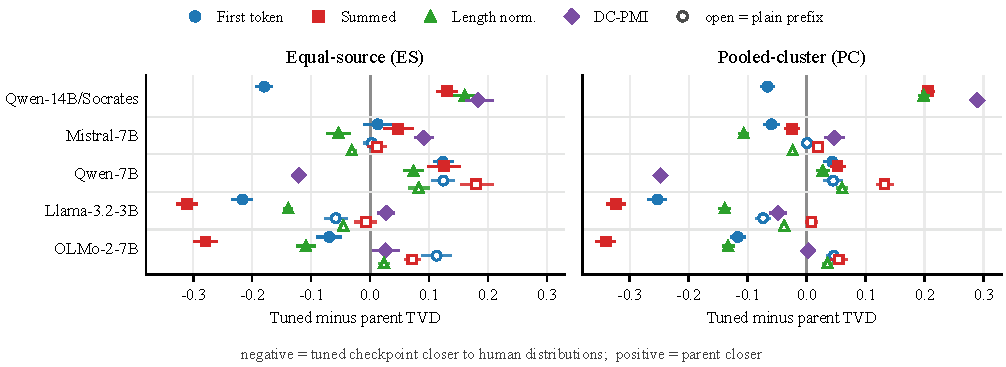
\includegraphics[width=.94\textwidth]{figures/fig_five_pair_gap_forest.pdf}
\caption{Original panel: tuned-minus-parent TVD for each pair and readout,
with 95\% cluster-bootstrap intervals; negative values favor the tuned
checkpoint. Filled markers: shared chat template (four readouts). Open
markers: shared plain prefix (three same-tensor readouts; Base--Instruct pairs
only).}
\label{fig:five-pair-gap}
\end{figure*}}
\newcommand{\fifteenforest}{%
\begin{figure*}[t]
\centering
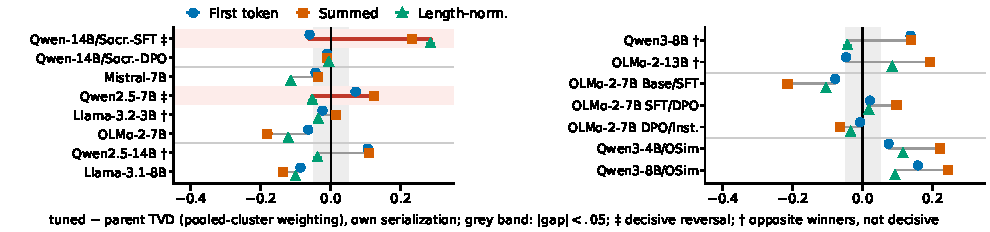
\includegraphics[width=\textwidth,height=1.25in]{figures/fig_fifteen_pair_gap_forest_wide.pdf}
\caption{Tuned-minus-parent TVD for all fifteen pairs (pooled-cluster weighting) under the three same-tensor readouts, each checkpoint in its own serialization; negative favors the tuned checkpoint; the grey band marks gaps below the .05 floor. A red connector ($\ddagger$) marks a decisive reversal between two readouts under \PC{} (Qwen-14B/Socrates-SFT and Qwen2.5-7B; Mistral-7B reverses decisively under \ES{} only); $\dagger$ marks opposite winners without both gaps at the floor. The same pairs under the shared chat template: Appendix Figure~\ref{fig:fifteen-both}.}
\label{fig:fifteen}
\end{figure*}}
\newcommand{\fifteenforestboth}{%
\begin{figure*}[t]
\centering
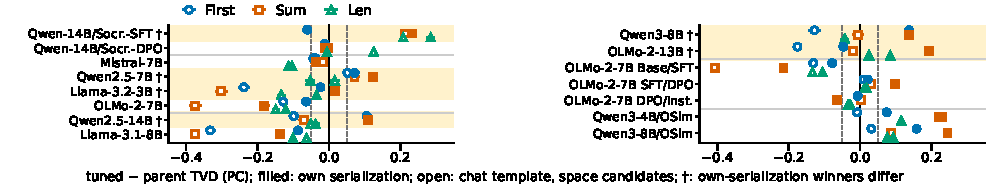
\includegraphics[width=\textwidth]{figures/fig_fifteen_pair_gap_forest_both.pdf}
\caption{Figure~\ref{fig:fifteen} with both conditions: each checkpoint in its own serialization (filled) and both under the chat template with space-prefixed candidates (open), pooled-cluster weighting, 95\% cluster-bootstrap intervals; shaded rows ($\dagger$): the own-serialization readouts give opposite winner letters under \PC{}.}
\label{fig:fifteen-both}
\end{figure*}}
\newcommand{\dicesfigure}{%
\begin{figure}[t]
\centering
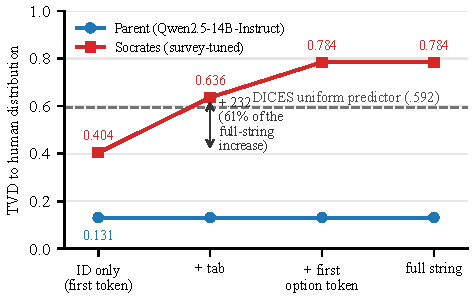
\includegraphics[width=\columnwidth]{figures/fig_dices_cumulative.pdf}
\caption{DICES loss of the Qwen-14B parent and Socrates as candidate tokens
are added to the scored string one position at a time (identical candidates
for both checkpoints; absent fourth tokens add zero). The first and last
points reproduce the first-token and summed readouts exactly. Paired
intervals are in Appendix Table~\ref{tab:qwen14-dices-token-decomposition}.}
\label{fig:dices}
\end{figure}}

\title{Same Models, Different Winner? What the Answer Readout Changes in Checkpoint Comparisons on SimBench}
\author{Anonymous ACL/ARR submission}
\date{}

\begin{document}
\maketitle

\begin{abstract}
Survey-simulation benchmarks compare a language model's distribution over a question's answer options with the distribution among human respondents. A model outputs token probabilities, not that distribution, so the evaluator must choose a \emph{readout}: which string to score, how to serialize the prompt, and how to reduce per-token scores to one score per option. We ask whether the readout changes which of two related checkpoints, a fine-tuned model and its parent, looks better. For fifteen checkpoint pairs on 2,038 SimBench items, both members of a pair see byte-identical prompts within each shared condition, and one stored tensor yields every reduction. Changing only the reduction reverses a decisive winner (opposite winners, both gaps at least .05 TVD) in about one comparison in four under the controlled shared template and one in eight under each checkpoint's own serialization, and half or more of those reversals involve a first-token readout that scores a token the model almost never produces (under a chat template with space-prefixed candidates, for example, such a readout reads at most 2\% of the probability mass for 28 of 30 checkpoint entries). Two public harnesses produce the same remainder, and the whitespace rule of one, replicated in our scorer, silently drops a prompt token for one tokenizer family; we release an opt-in patch. Scoring the option text instead of the ID--option string changes more comparisons, the only difference that is separable with ten model families and only under the shared template, but that string is itself a remainder readout; a full-mass label string, the source composition, and the sharpness of the predictions change comparisons about as often as the reduction. A survey-fine-tuned checkpoint that loses under full-string readouts through a habit at one token wins under its own protocol, by a margin that is mostly spread. We close with six reporting practices.
\end{abstract}

\section{Introduction}

A growing line of work uses language models to simulate how groups of people
answer survey questions
\cite{argyle2023out,santurkar2023opinions,durmus2024globalopinionqa,
hu-etal-2026-simbench}. The model is shown a question and its answer options,
and its predicted distribution over the options is compared with the human respondents' distribution. Benchmarks such as SimBench
score the comparison with total variation distance (TVD), the share of
probability mass that would have to move to turn one distribution into the
other. The scores rank models and support claims that fine-tuning on human
response data improves simulation
\cite{kolluri-etal-2025-finetuning,suh2025subpop,cao-etal-2025-specializing}.

A language model does not, however, output a distribution over answer
options. It outputs probabilities over tokens, and the evaluator has to decide
how to read an answer off. One can score an option's first token, its whole string, or the string averaged per token; correct the score with a content-free prompt (DC-PMI; \citealp{holtzman-etal-2021-surface}); sample answers; or ask the model to write a probability vector. Each rule yields a different distribution, and such choices are known to move absolute scores and leaderboards \cite{shen-etal-2025-revisiting,tsvilodub2024predictions,lyu-etal-2024-beyond}. Whether they move the comparison that fine-tuning claims rest on, the gap between a checkpoint and its parent, has not been isolated.

We isolate it with a controlled audit (Figure~\ref{fig:readouts}). Within each shared-template condition both checkpoints of a pair see byte-identical prompts, and one teacher-forced pass stores the per-token log-probabilities from which every reduction is computed, so two reductions differ only in arithmetic on the same numbers. We apply the design to a survey-fine-tuned checkpoint (Socrates; \citealp{kolluri-etal-2025-finetuning}) and four Base--Instruct pairs, then re-implement the pipeline from its written specification and extend it to fifteen pairs from ten model families, four serialization conditions, and generated-answer readouts. Our contributions:
\begin{itemize}[leftmargin=*,itemsep=1pt,topsep=2pt]
\item \textbf{An audit design for paired comparisons}: shared bootstrap draws, so that every interval is paired, and a token-by-token trace of any change of gap between two reductions (Section~\ref{sec:design}).
\item \textbf{An account of what changes a winner} (Table~\ref{tab:what-changes}): changing only the reduction reverses a decisive winner in at most one comparison in four, mostly through remainder readouts; scoring the option text changes more but is itself a remainder readout; a full-mass label string, the serialization, the source composition, and the sharpness change about as many (Section~\ref{sec:reduction}).
\item \textbf{A coverage diagnostic} showing that first-token scoring under a chat template with space-prefixed candidates reads a small remainder of the probability mass, the harness whitespace rules behind it, and an opt-in harness patch (Section~\ref{sec:coverage}).
\item \textbf{Two survey-fine-tuned families under their own protocols}, showing that a reported loss can be a format artifact at a single token (Section~\ref{sec:socrates}).
\end{itemize}

\section{Background and Related Work}

\paragraph{Survey simulation.}
Since early ``silicon sampling'' studies \cite{argyle2023out,aher2023using},
model--human alignment has been measured from populations to individuals
\cite{santurkar2023opinions,durmus2024globalopinionqa,suh2025subpop,
cao-etal-2025-specializing,wang-etal-2025-sociobench,park2024generative,
bisbee2024synthetic,tjuatja2024biases,
dominguez-olmedo-etal-2024-questioning,williams-etal-2026-beyond,
libovicky-2026-credibility}, and whether such samples can stand in for respondents is contested \cite{dillion2023replace,boelaert2025machine,anthis2025llm}. SimBench
\cite{hu-etal-2026-simbench} unifies 20 datasets and scores next-token label
probabilities for base models and verbalized distributions for
instruction-tuned models \citep[see also][]{meister-etal-2025-benchmarking,ahnert-etal-2026-survey,hu-levy-2023-prompting},
and fine-tuning on human data is reported to improve alignment
\cite{kolluri-etal-2025-finetuning,suh2025subpop,krsteski-etal-2026-valid,
huang-etal-2026-distribution}.

\paragraph{Reading answers off a language model.}
Multiple-choice scoring is sensitive to what is scored: raw likelihood,
length normalization, and DC-PMI respond differently to surface-form
competition \cite{holtzman-etal-2021-surface}, and label, sequence, and
generation-based scoring change rankings
\cite{robinson2023leveraging,shen-etal-2025-revisiting,tsvilodub2024predictions,lyu-etal-2024-beyond};
HELM and OLMES standardize these choices
\cite{liang2022helm,gu-etal-2025-olmes,biderman2024lessons}. Label priors and
option order \cite{zhao2021calibrate,zheng2024mcq,pezeshkpour-hruschka-2024-large},
formatting \cite{sclar2024quantifying,alzahrani-etal-2024-benchmarks,
mizrahi-etal-2024-state}, first-token versus generated answers
\cite{wang-etal-2024-answer-c,wang2024look}, leading spaces
\cite{sanz-guerrero-etal-2025-mind}, and format fine-tuning \cite{bunn-etal-2025-format} are known sensitivities; human label variation \cite{plank-2022-problem,uma2021learning,nie-etal-2020-learn} is the same distributional target seen from the annotation side.

\paragraph{What is new here.}
Readout sensitivity is not new \citep{fourrier2023openllm,shen-etal-2025-revisiting,schaeffer2023emergent,dehghani2021benchmark}, and OLMES and lm-evaluation-harness \cite{eval-harness} compute several readouts from one tensor. We apply this discipline, a multiverse analysis \citep{steegen2016multiverse,simonsohn2020specification}, to \emph{paired} checkpoint gaps on a distributional task with a token-by-token trace of each gap change, turn the label-mass analyses of \citet{wang-etal-2024-answer-c} and \citet{sanz-guerrero-etal-2025-mind} into a coverage statistic, and retain invalid outputs through partial-identification bounds \cite{manski1989anatomy,chen2026partial}.

\section{Audit Design}
\label{sec:design}
\begin{figure}[t]
\centering
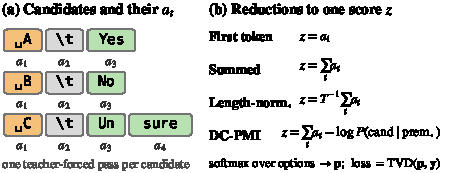
\includegraphics[width=\columnwidth]{figures/fig_readouts.pdf}
\caption{Within a shared-template condition both checkpoints see byte-identical prompts. (a)~One teacher-forced pass records a log-probability $a_t$ per candidate token; (b)~the same-tensor readouts differ only in how the $a_t$ are reduced.}
\label{fig:readouts}
\end{figure}

\begin{table}[t]
\centering\scriptsize
\setlength{\tabcolsep}{3pt}
\begin{tabular}{@{}>{\raggedright\arraybackslash}p{1.9cm}p{5.55cm}@{}}
\toprule
Term & Meaning \\
\midrule
Scored string (event) & What is scored: ``\texttt{ID<TAB>option}'' (default), the option text alone, or the ID alone. \\
Serialization & How the prompt becomes tokens: the shared chat template (space or no-space candidates), the shared plain prefix, or each checkpoint's own serialization. \\
Reduction & How per-token scores become one score: first token, sum, or per-token mean (the three \emph{same-tensor} readouts, computed from one stored tensor), character-normalized, or DC-PMI. \\
Unit; changed, flipped, decisive & One pair under one weighting (30 units); two readouts change it when their winners differ, flip it when the winners are opposite with a paired difference of at least .05 TVD, and reverse it decisively when the winners are opposite and both gaps are at least .05. \\
Coverage, remainder & Mass at the label position on the distinct first candidate tokens; full-mass at .5 or more, a remainder below .05. \\
\bottomrule
\end{tabular}
\caption{Terms used in the paper; the readout is the triple (scored string, serialization, reduction).}
\label{tab:glossary}
\end{table}

Table~\ref{tab:glossary} collects the terms; each is defined where it first appears.

\subsection{Checkpoint pairs and data}
\label{sec:pairs}

Each pair has a \emph{parent} and a \emph{tuned} checkpoint, and its gap $\Delta = L_{\mathrm{tuned}} - L_{\mathrm{parent}}$ is the tuned checkpoint's loss minus the parent's, so a negative gap favors the tuned checkpoint. The
original panel has five pairs: Qwen2.5-14B-Instruct and Socrates, a checkpoint
fine-tuned from it on individual-level responses to social-science experiments
\cite{qwen25technical,kolluri-etal-2025-finetuning}, and the Base and Instruct
releases of Mistral-7B-v0.3 \cite{jiang2023mistral}, Qwen2.5-7B
\cite{qwen25technical}, Llama-3.2-3B \cite{meta2024llama32}, and OLMo-2-1124-7B
\cite{olmo2024furious}. The extended panel adds ten pairs: a
Socrates checkpoint trained with DPO on the same data; Base--Instruct pairs of
Qwen2.5-14B, Llama-3.1-8B, Qwen3-8B, and OLMo-2-13B; the three steps of the
OLMo-2-7B post-training ladder (Base--SFT, SFT--DPO, DPO--Instruct); and two
behavioral mid-training checkpoints, OSim-mid, trained from Qwen3-4B-Base and
Qwen3-8B-Base on a mixture that includes Socrates' training data
\cite{zhou-etal-2026-odyssim}. A sixteenth pair, Mistral-7B-v0.1 and its SubPOP adapter \cite{suh2025subpop}, is scored under the plain prefix (Section~\ref{sec:socrates}) and kept outside the counts, which refer to the fifteen pairs (23 distinct checkpoints from ten families; Qwen2.5-14B-Instruct appears in three pairs and two families). Each pair uses the tuned checkpoint's tokenizer and template (the parent's for the Socrates pairs; the OSim checkpoints ship Qwen3's).

SimBench \cite{hu-etal-2026-simbench} provides, for each item, a group
description, a question, an ordered list of answer options, and the human
answer distribution. We use its population-level split and five of its
twenty sources, chosen by a license rule before any model was run (Appendix~\ref{app:sources}): the European Social Survey (ESS), GlobalOpinionQA, the
DICES conversational-safety ratings, the NumberGame concept-generalization
task, and a conspiracy-belief survey (ConspiracyCorr)
\cite{ess-round8-2016,ess-round9-2018,ess-round10-2020,durmus2024globalopinionqa,
aroyo2023dices,bigelow2016numbergame,enders2024conspiracism}. Two of the five are behavioral rather than opinion data: DICES and NumberGame supply 998 of the 1,680 clusters and 59\% of the pooled-cluster weight, so the opinion sources are also analyzed on their own (Appendix~\ref{app:reimpl}), and ISSP and Jester are held out. An \emph{item} is one rendered group--question input with its $K_i$ ordered options and human distribution; items sharing question and options form a \emph{cluster}. Four GlobalOpinionQA items whose shares do not sum to 100 are excluded, leaving 2,038 items in 1,680 clusters (Appendix Table~\ref{tab:frame}); this fixed item set is the \emph{frame} every loss averages over.

\subsection{Readouts}
\label{sec:reductions}

Within a pair, both checkpoints receive the same system message, rendered
group, question, option list, answer prefix, and tokenizer
(Appendix~\ref{app:prompts}). Candidate $k$ is the byte string
``\texttt{\char32 ID$_k$<TAB>option$_k$}''. One teacher-forced pass records,
for checkpoint $e$, item $i$, option $k$, and candidate-token position $t$,
the log-probability $a_{eikt}$ of the actual next token; $T_{ik}$ is the
number of candidate tokens. The three same-tensor scores are the first token, $z^{\textsc{first}}_{eik}=a_{eik1}$; the sum, $z^{\textsc{sum}}_{eik}=\sum_{t=1}^{T_{ik}} a_{eikt}$; and the per-token mean, $z^{\textsc{len}}_{eik}=T_{ik}^{-1}\sum_{t=1}^{T_{ik}} a_{eikt}$. Each passes through a temperature-1 softmax over the $K_i$ options. Because the softmax depends only on score differences, a change in gap between two readouts can be traced token by token through cumulative-prefix scores whose increments sum exactly to the total change. The fourth readout, domain-conditional PMI (DC-PMI), subtracts from the summed score the log-probability of the same candidate under a content-free premise that keeps the system message and chat template but omits the group, question, and option list \citep{holtzman-etal-2021-surface,zhao2021calibrate}: $z^{\textsc{pmi}}_{eik}=z^{\textsc{sum}}_{eik}-\log P_e(c_{ik}\mid d)$. Public harnesses compute the same quantities under other names, such as lm-evaluation-harness's \texttt{acc} and \texttt{acc\_norm} (Appendix Table~\ref{tab:harness-names}).

The \emph{serialization} is how the prompt becomes tokens. Scoring both checkpoints under the Instruct chat template with space-prefixed candidates keeps the prompt identical, but it is not how either checkpoint is normally used (Section~\ref{sec:coverage}). Table~\ref{tab:what-changes} therefore reports four serialization conditions, in the order of its columns. The first is each checkpoint's \emph{own serialization}: a Base parent under the plain prefix with space candidates, its tuned checkpoint under the chat template without a space, so the two see different prompts. The second is the shared template with candidates that carry no leading space. The third is the same template with space-prefixed candidates, the condition we specified in advance; the no-space condition is its correction after the coverage diagnosis. The fourth is a shared plain prefix without chat markup, under which most checkpoints keep at least half of their mass on the label tokens. Where one number is needed we quote the no-space column (controlled) or own serialization (normal use). The \emph{scored string} (the event rows of Table~\ref{tab:what-changes}) is what is scored: the ``\texttt{ID<TAB>option}'' string by default, the option text alone, or the ID alone. Generated-answer readouts complement the likelihood readouts (Appendix~\ref{app:prompts}): SimBench's next-token readout, verbalized vectors (the model writes a probability vector) under two prompts, sampled answers, and Socrates' native protocol. A \emph{label readout} scores a one-token label by its first token.

\subsection{Loss, weighting, and what we count}
\label{sec:weights}

For human distribution $\mathbf y_i$ and model distribution $\mathbf p_{ei}$,
the loss is $\ell_{ei}=\TVD(\mathbf p_{ei},\mathbf y_i)=
\tfrac12\sum_k|p_{eik}-y_{ik}|$, averaged over items within a cluster, then
over clusters within a source. \emph{Equal-source} (\ES{}) weighting gives
each source one fifth of the weight; \emph{pooled-cluster} (\PC{}) weighting
gives every cluster the same weight. \PC{} is primary (\ES{} lets ConspiracyCorr's nine clusters count as much as DICES' 498); both are reported. A uniform predictor gives the absolute baseline (TVD .356 under \ES{}, .394 under \PC{}). Because TVD rewards matching spread, we also report modal accuracy (whether the predicted mode is the human mode),
within-item Spearman correlation, and an entropy-matched variant whose
temperature, fitted on the other sources, gives each checkpoint the human
answers' spread.

A \emph{unit} is one pair under one weighting (30 units), a \emph{cell} one unit under one readout, and each readout names a winner for a unit: the side its 95\% interval favors (written as that side's letter), or a tie ($\circ$) when the interval includes zero. Two readouts \emph{change} a unit when they name different winners, a tie included; they \emph{flip} it when they name opposite sides and the paired difference between the two gaps is at least .05 TVD; the change is \emph{decisive} when they name opposite sides and both gaps are at least .05. \emph{Coverage} is the probability mass a checkpoint places, at the prefix-final position, on the distinct first candidate tokens; a label readout is full-mass at .5 or more and a \emph{remainder} below .05. As a worked example, take the Mistral-7B pair in own serialization. Under \ES{} weighting the first-token and summed readouts put the Base parent ahead by .067 and .068 TVD while the length-normalized readout puts Instruct ahead by .052: the winners are opposite and both gaps exceed .05, so this unit counts as changed and as a decisive reversal. Under \PC{} weighting all three readouts favor Instruct (by .043, .037, and .114), so that unit does not change.

\subsection{Uncertainty and execution}
\label{sec:execution}

Every checkpoint is evaluated once, deterministically, so the only sampling
uncertainty we quantify is over items: 10,000 cluster-bootstrap resamples within each source \citep{field2007bootstrapping,miller2024adding}, with one set of draws shared
across both checkpoints and all readouts of a pair, so that all intervals are
paired. The .05 decisive floor was fixed before the extended panel was run; it is about twice the cross-implementation floor of .027, and by a power simulation it operates at about .06 (a true reversal of $\pm.06$ is detected in 85\% of resampled frames, one of $\pm.05$ in a tenth). Differences between rows of Table~\ref{tab:what-changes} are judged by a paired bootstrap over the ten model families and by an exact sign-flip test over the per-family contributions, whose smallest attainable $p$ is $2/2^k$ when $k$ families contribute; we call a difference \emph{separable} when the interval excludes zero and the test rejects at .05. The no-space, plain-prefix, and own-serialization columns, the coverage and above-uniform gates of Section~\ref{sec:reduction}, the family bootstrap, and the human reference were specified after the pre-specified column's counts were known (Appendix Table~\ref{tab:timing}), so comparisons between rows are descriptive. Every count's robustness to the floor, the loss, the respondent count, and family resampling is in Appendix~\ref{app:reimpl} (Table~\ref{tab:appendix-index}).

Every result in Section~\ref{sec:results} comes from a same-team re-implementation written from Appendix~\ref{app:prompts}, run with AI assistance in a separate session; it reproduces the original panel's decisive comparisons cell for cell, with losses within .027 TVD (the original numbers were visible during that check; Appendix~\ref{app:compute}). No human distribution enters a prompt (except the five held-out modes of the few-shot diagnostic, Appendix Table~\ref{tab:fewshot}), and there is no prompt search.

\section{Results}
\label{sec:results}

\subsection{What changes a winner}
\label{sec:reduction}

\begin{table*}[t]
\centering\scriptsize
\setlength{\tabcolsep}{4pt}
\begin{tabular}{@{}lrrrrrrrrrrrr@{}}
\toprule
& \multicolumn{3}{c}{Own serialization} & \multicolumn{3}{c}{Shared, no-space cand.} & \multicolumn{3}{c}{Shared, space (pre-spec.)} & \multicolumn{3}{c}{Shared plain prefix} \\
\cmidrule(lr){2-4}\cmidrule(lr){5-7}\cmidrule(lr){8-10}\cmidrule(l){11-13}
What is varied & Chg. & Dec. & $|\Delta|$ & Chg. & Dec. & $|\Delta|$ & Chg. & Dec. & $|\Delta|$ & Chg. & Dec. & $|\Delta|$ \\
\midrule
Reduction: any of three & 13 & 4 & .09 & 14 & 7 & .10 & 14 & 3 & .10 & 14 & 1 & .05 \\
Reduction: any of four & 16 & 8 & .09 & 15 & 10 & .09 & 15 & 4 & .09 & 16 & 1 & .04 \\
Event: option text & 20 & 8 & .12 & 26 & 10 & .12 & 24 & 12 & .17 & -- & -- & -- \\
Event: ID only & 13 & 5 & .08 & 15 & 8 & .11 & 15 & 5 & .10 & -- & -- & -- \\
Serialization: chat$\to$plain & -- & -- & -- & 23 & 7 & .10 & 21 & 4 & .10 & -- & -- & -- \\
Sharpness: matched $T$ & 11 & 1 & .07 & 13 & 5 & .08 & 19 & 5 & .08 & 20 & 1 & .05 \\
Frame: omit DICES & 18 & 3 & .07 & 12 & 3 & .07 & 14 & 1 & .07 & 17 & 1 & .04 \\
Loss: TVD$\to$Brier & 9 & 0 & -- & 8 & 0 & -- & 10 & 0 & -- & 9 & 0 & -- \\
Weighting (15 pairs) & 9 & 0 & .05 & 7 & 1 & .05 & 7 & 1 & .05 & 6 & 0 & .02 \\
\bottomrule
\end{tabular}
\caption{What changes a winner: pair--weighting units (15 pairs $\times$ 2 weightings; the weighting row counts pairs) whose winner symbol changes (Chg.) or reverses decisively (Dec.: opposite winners, both gaps at least .05 TVD) when the named element is varied, and the mean absolute change of the paired gap ($|\Delta|$, TVD). Conditions: own serialization; the shared chat template with no-space and with space-prefixed candidates (the latter pre-specified; first-token scoring reads a remainder there); the shared plain prefix, where both checkpoints keep at least half of their mass on the label tokens in 25 of 30 units. Decisive reversals under the reduction per family: 3, 4, and 2 of 10 (first three conditions). Reduction rows compare the three same-tensor readouts, or four with the character-normalized one; other rows compare each same-tensor readout with the named change; the frame row is the largest of five single-source omissions (first three conditions: median 6, 8, and 10 changed; only DICES reverses decisively; under the plain prefix only the DICES omission was run). Full row set, flips, pair and family counts, and intervals: Appendix Tables~\ref{tab:what-changes-full}, \ref{tab:pair-family-counts}, \ref{tab:family-boot}, \ref{tab:family-boot-events}.}
\label{tab:what-changes}
\end{table*}


\paragraph{Changing only the reduction rarely reverses a large gap, but how rarely depends on the condition.} Across the three same-tensor readouts, about half of the 30 units change winner in every condition, many of them among small gaps. Decisive reversals are rarer: 4 of 30 in own serialization, 7 under the controlled shared template with no-space candidates (4 of 15 pairs), 3 with space-prefixed candidates, and 1 under the plain prefix (Figure~\ref{fig:fifteen}). The family-bootstrap intervals on these counts are wide ([0,9], [2,15], and [0,8] units in the first three conditions), so the panel bounds the rate rather than pins it, and the count moves with the criterion: adding the character-normalized readout raises the decisive counts to 8, 10, and 4 (the plain count stays at 1), the Brier score to 8, 10, and 8 (first three conditions), and the paired-difference criterion counts 9, 10, 9, and 4 flips (Appendix Tables~\ref{tab:what-changes-full}, \ref{tab:pair-family-counts}, \ref{tab:proper-scores}). Most of these reversals are not well posed: of the 4, 7, 3, and 1 decisive reversals, 2, 4, 2, and 1 involve a first-token readout whose coverage is below .05, and when both checkpoints clear a coverage of .5 the reduction reverses one unit of 26 in own serialization, two of 8 with no-space candidates, and none of 25 under the plain prefix; with both checkpoints also beating a uniform predictor (4 to 6 units per condition) at most one reverses. Without Qwen2.5-7B, whose gaps move by up to .135 under FP32, the counts fall by at most two; the largest movement between two reductions is .41 TVD (OLMo-2-13B, no-space candidates, summed minus first token; Appendix Tables~\ref{tab:own-absolute}, \ref{tab:gap-changes-15}).

\paragraph{Which string is scored changes more comparisons.} Scoring the option text alone instead of the ``\texttt{ID<TAB>option}'' string changes 20, 26, and 24 units (8, 10, and 12 decisively) against the reduction's 13, 14, and 14 (first three conditions). The advantage is separable under the shared template but not in own serialization, and it rests on few families: the sign-flip $p$ of .03 is the test's floor with six contributing families, and it rises to .06 and .09 if Qwen2.5-14B-Instruct's two families are merged into nine, and to .06 for the matched-instruction variant of the string (Appendix Tables~\ref{tab:family-boot-diff-merged}, \ref{tab:family-boot-events}). The text-only string is, however, a remainder readout everywhere: its first-token coverage is at most .19 (Appendix Table~\ref{tab:events-coverage}), and full-string coverage cannot exceed it. Comparing one change of reduction against one change of string without the first token, the string still changes more units under the shared template ($+12$ to $+13$, $p\le.03$) but in own serialization only under the length-normalized readout, and not separably (Appendix Table~\ref{tab:matched-contrast}). The one alternative string that is full-mass in the same condition as the default string, the ID alone in own serialization (25 of 30 entries at .5 or more), changes 13 units and 5 decisively, about as many as the reduction (13 and 4).

\paragraph{Source composition and sharpness change as many comparisons, and sharpness leads on opinion items.} Omitting DICES, one of the two 500-item sources, changes 18, 12, 14, and 17 units (3, 3, 1, and 1 decisively), about as many as the reduction and no more decisively; the other single-source omissions change 2 to 11 units, none decisively (Appendix Table~\ref{tab:frame-per-omission}). Matching each checkpoint's sharpness to the human answers' entropy changes 11, 13, 19, and 20 units (1, 5, 5, and 1 decisively) in the main frame, but on the two opinion sources alone it changes more units than any other manipulation (28, 21, and 26, with 12, 12, and 11 decisive; Appendix Table~\ref{tab:opinion-events}), and likewise on the items with at least 100 respondents. Neither lever, nor the serialization, is separable from the reduction (Appendix Table~\ref{tab:family-boot-diff}).

Two caveats apply to every count: winner counts miss magnitude (Appendix Table~\ref{tab:magnitude-crossing}), and manipulations act through pair-specific responses (a sum-of-squares partition attributes 51\% of the variance in gaps to pair identity and 2.5\% to the readout main effect). Appendix~\ref{app:reimpl} collects every row, interval, and recount, indexed by claim in Table~\ref{tab:appendix-index}.

\fifteenforest
\subsection{First-token scoring under a chat template reads a remainder}
\label{sec:coverage}

After the assistant header a chat model writes no space, so under the shared chat template, where every candidate begins with a space, ``\texttt{\char32 A}'' is a token it almost never produces there: coverage is .02 or less for 28 of the 30 checkpoint entries (15 pairs, two members each; Appendix Table~\ref{tab:coverage}). With no-space candidates the eight Instruct checkpoints are at .90 to 1.00 but their Base parents at .01 to .57; under the plain prefix seven of the eight Base parents keep at least half of their mass. Full-string readouts do not restore the mass: under the chat template the total probability of the $K_i$ candidate strings is at most .021 for every entry but Mistral-Instruct (Appendix Table~\ref{tab:fullstring-coverage}), so summed and length-normalized scores compare continuation likelihoods, not answer mass. One in-context demonstration restores coverage in five of six pair--serialization conditions but moves gaps by up to .31 TVD (Appendix Table~\ref{tab:fewshot}).

The remainder is a harness property as much as a renderer property. With a chat template OLMES puts a space before the choice and lm-evaluation-harness none \cite{eval-harness,sanz-guerrero-etal-2025-mind}, and both move the template's trailing whitespace onto the continuation and encode prefix and candidate jointly. Run unmodified on three pairs, they reproduce our coverage to within .05 for 11 of the 12 checkpoint entries (the exception is a no-space Mistral-7B-Instruct cell whose candidate lacks SentencePiece's word-boundary marker) and our summed winners in 11 of the 12 harness winner cells.

For the Qwen2.5-7B pair the prefix ends in \texttt{<|im\_start|>assistant\textbackslash n}, so the scored ids of the second candidate are 198, 425, 197 (\texttt{\textbackslash n}, \texttt{\char32 B}, \texttt{\textbackslash t}): the newline, identical for every candidate, is scored first, a label readout taken there is uniform, and the label is scored second; this happens for 9 of the 15 pairs. For the harness's summed score (\texttt{acc}) the newline's log-probability cancels in the softmax over options, so the summed winners of those nine pairs are unchanged; what the rule changes is \texttt{acc\_norm}, whose divisor varies across candidates, and any label or first-token readout. For the five OLMo-2 pairs the joint encoding fuses the newline with the prefix's last token, so the slice starts at the label and the model is conditioned on the separately encoded prefix without the newline, a change to the prompt itself (Appendix Table~\ref{tab:joint-example}). Replicated on all fifteen pairs (the harness runs cover three pairs, none of them OLMo-2), the rule changes 4 of 30 units under the summed or length-normalized readout, none decisively, but moves the OLMo-2-7B summed gaps by up to .28 and reverses the OLMo-2-13B summed \PC{} gap ($-.020$ to $+.153$). We release an opt-in patch for lm-evaluation-harness that keeps the trailing whitespace in the prefix (or moves only spaces, never newlines), counts the requests whose joint encoding breaks the prefix boundary, and writes per-token scores, from which the first-token readout and coverage follow; with its options off it reproduces the unpatched harness exactly (Appendix~\ref{app:harness-patch}).

\subsection{Two survey-fine-tuned families under their own protocols}
\label{sec:socrates}

\begin{table}[t]
\centering\scriptsize
\setlength{\tabcolsep}{2pt}
\begin{tabular}{@{}lrrrrrr@{}}
\toprule
& \multicolumn{2}{c}{Parent} & \multicolumn{2}{c}{Socrates-SFT} & \multicolumn{2}{c}{Socrates-DPO} \\
\cmidrule(lr){2-3}\cmidrule(lr){4-5}\cmidrule(l){6-7}
Readout & ES & PC & ES & PC & ES & PC \\
\midrule
\multicolumn{7}{@{}l}{\emph{Same-tensor, letter IDs, chat template}} \\
First token & \textcolor{gray}{\textit{.475}} & \textit{.362} & \textit{.298}$^{S}$ & \textit{.301}$^{S}$ & \textcolor{gray}{\textit{.428}}$^{D}$ & \textit{.350}$^{D}$ \\
Summed & \textcolor{gray}{.476} & .362 & \textcolor{gray}{.611}$^{P}$ & \textcolor{gray}{.575}$^{P}$ & \textcolor{gray}{.434}$^{D}$ & .359$^{\circ}$ \\
Length-normalized & \textcolor{gray}{.423} & .380 & \textcolor{gray}{.588}$^{P}$ & \textcolor{gray}{.588}$^{P}$ & \textcolor{gray}{.488}$^{P}$ & \textcolor{gray}{.505}$^{P}$ \\
DC-PMI & \textcolor{gray}{.507} & \textcolor{gray}{.398} & \textcolor{gray}{.691}$^{P}$ & \textcolor{gray}{.688}$^{P}$ & \textcolor{gray}{.609}$^{P}$ & \textcolor{gray}{.550}$^{P}$ \\
\multicolumn{7}{@{}l}{\emph{Same-tensor, integer IDs (no leading space)}} \\
First token & \textcolor{gray}{.459} & .367 & .288$^{S}$ & .295$^{S}$ & \textcolor{gray}{.440}$^{D}$ & .355$^{D}$ \\
Summed & \textcolor{gray}{.461} & .369 & \textcolor{gray}{.496}$^{P}$ & \textcolor{gray}{.410}$^{P}$ & \textcolor{gray}{.442}$^{D}$ & .357$^{D}$ \\
Length-normalized & \textcolor{gray}{.366} & .307 & \textcolor{gray}{.571}$^{P}$ & \textcolor{gray}{.561}$^{P}$ & .330$^{D}$ & .300$^{\circ}$ \\
\multicolumn{7}{@{}l}{\emph{Same-tensor, option text only (no ID)}} \\
First token & \textcolor{gray}{\textit{.544}} & \textcolor{gray}{\textit{.528}} & \textit{.316}$^{S}$ & \textit{.300}$^{S}$ & \textcolor{gray}{\textit{.419}}$^{D}$ & \textit{.376}$^{D}$ \\
Summed & \textcolor{gray}{.577} & \textcolor{gray}{.538} & \textcolor{gray}{.438}$^{S}$ & .330$^{S}$ & \textcolor{gray}{.447}$^{D}$ & .392$^{D}$ \\
Length-normalized & \textcolor{gray}{.594} & \textcolor{gray}{.556} & \textcolor{gray}{.476}$^{S}$ & .368$^{S}$ & \textcolor{gray}{.501}$^{D}$ & \textcolor{gray}{.418}$^{D}$ \\
\multicolumn{7}{@{}l}{\emph{Native integer protocol, exact next-token probabilities}} \\
Exact, $T{=}1$ & \textcolor{gray}{.450} & .364 & .291$^{S}$ & .299$^{S}$ & \textcolor{gray}{.435}$^{D}$ & .353$^{D}$ \\
\multicolumn{7}{@{}l}{\emph{Generated answers}} \\
SimBench next-token & \textcolor{gray}{.507} & \textcolor{gray}{.406} & \textit{.312}$^{S}$ & \textit{.316}$^{S}$ & \textcolor{gray}{.464}$^{D}$ & \textcolor{gray}{.402}$^{\circ}$ \\
Verbalized JSON & .214 & .202 & inv. & inv. & .215$^{\circ}$ & .212$^{P}$ \\
\bottomrule
\end{tabular}
\caption{Qwen2.5-14B-Instruct and its two Socrates checkpoints under every readout (re-implementation runs; all-source TVD, uniform baseline .356 ES / .394 PC). Superscripts: winner against the parent by the 95\% interval of the paired gap (S = Socrates-SFT, D = Socrates-DPO, P = parent, $\circ$ = includes zero). Italic: remainders, where the scored first token carries under .05 of the mass for all three checkpoints (the space-prefixed letter IDs and the text-only event; Appendix Tables~\ref{tab:coverage}, \ref{tab:events-coverage}) or for Socrates-SFT alone (SimBench next-token); with integer IDs and no leading space all three place essentially all of their mass on the label tokens (coverage at least .999; Appendix Table~\ref{tab:coverage})). Grey: worse than the uniform predictor. Exact native rows: each complete answer ``$k$\texttt{<|im\_end|>}'' under Socrates' own prompt (captured mass .9997, .9999, and .54) at $T{=}1$; ``inv.'': no valid output; gaps in the text are computed before rounding. Sampled readouts: Appendix Table~\ref{tab:generation}.}
\label{tab:socrates-readouts}
\end{table}


Socrates was trained to answer with an integer, so the letter-ID candidates
of the shared prompt are a format it never saw.
In Table~\ref{tab:socrates-readouts} the readouts that favor the parent are those in which the scored string continues past an answer ID: summed and
length-normalized scoring with letter IDs ($+.213$, $+.208$ under \PC{}) or integer IDs, and DC-PMI, in all of which Socrates is worse than a uniform predictor. With integer IDs and no leading space, Socrates' own format (unlike its own serialization, which uses letter IDs), both checkpoints place essentially all of their mass on the label tokens (coverage at least .999; Appendix Table~\ref{tab:coverage}); there the first-token readout favors Socrates and the summed readout, which continues past the ID, favors the parent. When the option text is scored on its own, Socrates wins under all three
reductions ($-.228$, $-.208$, $-.188$), and it wins the exact version of its native protocol by $-.159$ (\ES{}) and $-.066$ (\PC{}), a margin that is mostly spread. The first-to-summed change shifts the Socrates gap by $+.274$ (\PC{}) through Socrates' own loss; a token-position trace (Appendix Figure~\ref{fig:dices} and Table~\ref{tab:positions-all}) locates 61\% of the DICES gap increase at the tab after the answer ID, which moves Socrates from better than uniform to worse. The penalty is concentrated on DICES ($+.673$ there; $+.000$ and $+.019$ without it) but recurs on both held-out sources, and only a reversed option order removes it (Appendix~\ref{app:diagnostics}). Socrates-SFT never writes a valid probability vector, so the benchmark's protocol for instruction-tuned models cannot score it at all.

A second survey-fine-tuned family, SubPOP \cite{suh2025subpop}, a LoRA adapter on Mistral-7B-v0.1 trained with lettered options, wins in all 48 cells of the readouts it can be scored under (raw and entropy-matched; $-.05$ to $-.18$ under \PC{}; Appendix Table~\ref{tab:subpop}), a matched interface where Socrates' is mismatched; its margin grows after entropy matching in 23 of the 24 readout--weighting cells, so it is preference rather than spread.

\subsection{Absolute fit and the benchmark's protocol}
\label{sec:absolute}

Comparative gaps do not certify a useful simulator: at temperature one, 112 of 180 same-tensor losses under the chat template and 79 of 180 in own serialization exceed the uniform baseline; on the items with at least 100 respondents 164 and 139 of 180 do, and no unit there has both checkpoints beating it under all three readouts (Appendix Table~\ref{tab:uniform-floor}). A human reference bounds what any predictor could reach: two fresh samples of the same size drawn from the published shares differ by .028 TVD on ESS, .040 on DICES, .116 on NumberGame, and .031 on ConspiracyCorr, whereas the lowest same-tensor loss of any checkpoint in its own serialization is .30, .11, .20, and .18 there (Appendix Table~\ref{tab:human-ceiling}). The Qwen-14B parent's written JSON vectors score .202 under \PC{}, better than every likelihood readout (Appendix Table~\ref{tab:generation}), and .183 on the four sources with respondent counts, 2.7 times their pooled reference of .068.

SimBench scores base models by next-token label probabilities and instruction-tuned models by verbalized vectors. Our renderer reproduces its prompts byte for byte but adds the assistant header for chat models, which the released token-probability code omits; run as released, that path moves the SimBench score (100 at a perfect match, 0 at the uniform predictor) by 24 to 76 points, and with the header the two agree; published chat-model scores use verbalized vectors and are unaffected (Appendix Table~\ref{tab:released-scorer}).

Under the next-token readout alone Base beats Instruct in five of the eight Base--Instruct pairs under \PC{} and six under \ES{}; under the benchmark's protocol with SimBench's prompt Instruct is closer in seven of the eight under \PC{} and three under \ES{}, with three ties and two Base wins. Instruct's next-token distributions are far sharper than Base's; after entropy matching four of the five Base wins disappear and modal accuracy favors Instruct in six, so the benchmark's own protocol, not the common next-token readout, agrees with the sharpness-matched and modal-accuracy verdicts (Appendix Tables~\ref{tab:protocol-audit}, \ref{tab:simbench-protocol}). On the two opinion sources alone the agreement weakens: Base wins all eight next-token comparisons; entropy matching hands five (\ES{}) or four (\PC{}) to Instruct; and the verbalized protocol gives Instruct four of seven under the controlled prompt (\PC{}) and one of eight under SimBench's prompt (four Base wins), though five of eight after entropy matching (Appendix Table~\ref{tab:protocol-opinion}). Such agreement between a protocol and a diagnostic is consistency, not validation.

\section{Recommendations}
\label{sec:recommendations}

\begin{enumerate}[leftmargin=*,itemsep=1pt,topsep=2pt]
\item \textbf{Name the scored string, pre-specify it, and match it to the checkpoint's protocol}: score each checkpoint under its own protocol and both under a shared full-mass string; a reported gain should survive both and be shown next to the uniform baseline and the human reference (Appendix Table~\ref{tab:human-ceiling}).
\item \textbf{Report the uniform baseline, the coverage at the label position, the encoding rule, and the space convention.} Check the convention by encoding the prefix alone and with the candidate (Appendix Table~\ref{tab:tokenization-boundary}); below .5 coverage report the checkpoint's own protocol or a shared full-mass string instead of a label readout; under a chat template keep the template's trailing newline in the prefix (the patch's \texttt{move\_only\_trailing\_spaces} or \texttt{keep\_trailing\_whitespace} option).
\item \textbf{Report every reduction the stored scores allow}: at least \texttt{acc}, \texttt{acc\_norm}, and \texttt{acc\_mutual\_info} (Appendix Table~\ref{tab:harness-names}) and, with the patch's per-token output, the first-token readout and coverage.
\item \textbf{Report a scale-free measure or a fitted temperature} next to TVD.
\item \textbf{Keep invalid outputs with bounds}, and report both weightings and leave-one-out results.
\item \textbf{Report the numerical precision and attention kernel, and rerun cells near the floor in FP32}; the arithmetic path moves one pair's gaps by up to .135 TVD.
\end{enumerate}
The scoring contract, task files, and patch are released under the MIT license (data terms in Appendix~\ref{app:sources}). In sum, the reduction rarely decides a comparison by itself; the scored string, the serialization, and the sharpness can; and a comparison is a statement about its readout until the readout is reported.

\FloatBarrier

\section*{Limitations}

\paragraph{Scope of the panel.}
Fifteen pairs and 23 distinct checkpoints are a convenience sample of publicly
released, locally runnable models. Three survey-fine-tuned checkpoints (Socrates-SFT and -DPO among the 23, and the SubPOP adapter on Mistral-7B-v0.1 in a sixteenth pair outside the counts) and two
behavioral mid-training checkpoints (OSim-mid) are the only ones trained on
human response data; SubPOP could be scored under the shared plain prefix
and SimBench's next-token readout but not under its own protocol, which
conditions on a demographic attribute question that SimBench's population
descriptions do not supply; no checkpoint of
\citet{cao-etal-2025-specializing} is released, and Gemma-2-9B was
inaccessible (gated repository). The pairs differ
in size, data, and recipe, so nothing here estimates the effect of a training
method in general; SubPOP differs from Socrates in parent type, adapter, and
label format, so its result shows that a survey-fine-tuned checkpoint need
not lose under the shared design, not that format alone explains Socrates,
and its training questions were not scanned for overlap. Our finding about Socrates is that it wins under its own
protocol and loses under a mismatched one; it rests on one SFT checkpoint
whose DPO sibling does not share the habit, its exact native margin shrinks
to .02 TVD after sharpness matching and is a tie under \ES{}, its native
prompt receives SimBench's group description in place of the individual
profile it was trained on, and we do not evaluate its reported gains on its
own benchmark. Nine extension checkpoints were loaded from their default
branch; the commits they resolved to are listed in Appendix
Table~\ref{tab:extension-revisions}.

\paragraph{Scope of the claims.}
No readout is a model-independent ground truth: first-token scoring is
distorted by label priors \cite{wang-etal-2024-answer-c,zheng2024mcq},
full-string scoring also measures wording, DC-PMI depends on its premise, and
verbalized distributions on format following; a study should choose the
readout that matches its claim, not the one under which its checkpoint
wins, and this audit ranks no readout by an external criterion of simulation quality; the no-space, plain-prefix, and own-serialization columns of Table~\ref{tab:what-changes} were added at revision, after the shared template's remainder had been diagnosed, without changing any count, and the space column is the pre-specified condition; Section~\ref{sec:absolute} adjudicates one class verdict by sharpness matching and modal accuracy, not the readouts themselves, and that verdict is itself weighting-dependent (Instruct seven of eight under \PC{}, three of eight with three ties under \ES{}).
Our results do not show that any training method helps or hurts in general,
nor that Socrates' reported gains are wrong. The frame is SimBench's
population-level split, whereas Socrates and SubPOP are trained as
subgroup or individual-level predictors, so their own use case is not
evaluated here; the text-only string's first-token readout is a remainder in every condition, so its counts rest on the summed and length-normalized readouts; and SubPOP is scored
only under serializations close to its training format.

\paragraph{Readouts and data.}
We cover likelihood readouts over ID--option strings, ID-only and text-only
candidates, DC-PMI under two premises, and the generated-answer readouts of Section~\ref{sec:reductions};
we do not cover chain-of-thought elicitation or constrained decoding. The
sampled readouts (50 integers at $T{=}.6$; 32 letters) carry Monte Carlo
noise and a fixed sampling temperature that the bootstrap does not model; the
exact native readout removes both for Socrates, and two further seeds move
the sampled gap by at most .005. Each control was run once with one seed and one paraphrase pair, except the option-order control (five seeds). No question of the seven sources used here appears
verbatim or as a near duplicate among the questions a fixed parser extracted
from Socrates' training data (Appendix~\ref{app:sources}); the unparsed rows
and OSim's mixture were not checked. The frame is
five SimBench sources, two of them behavioral with 59\% of the pooled-cluster
weight, and it excludes OpinionQA, Afrobarometer, and Latinobar\'ometro, so
it is not representative of opinion surveys (Appendix
Tables~\ref{tab:opinion-subset}, \ref{tab:opinion-issp}, and
\ref{tab:opinion-frame-changes} are the relevant check); equal-source
weighting gives ConspiracyCorr's nine clusters one fifth of the weight, and
Appendix Table~\ref{tab:flip-accounting} shows which cells depend on a
single source. The held-out check uses two further sources (ISSP and Jester; MoralMachine's option layout was not parsed
by the fixed renderer and was excluded rather than guessed). SimBench's
population-level human shares are treated as fixed targets except in the
respondent-resampling check of Appendix~\ref{app:resampling} and the human
reference of Appendix Table~\ref{tab:human-ceiling}, which assume simple random sampling, and TVD
rewards matching spread as well as preference, which is why we add
scale-free and entropy-matched measures rather than replace TVD.

\paragraph{Uncertainty and numerics.}
Cluster-bootstrap intervals capture sensitivity to which questions are in the
frame, not uncertainty over sources, prompts, or training. Absolute losses
reproduce across implementations only to about .03 TVD under bfloat16
arithmetic, and per-item vectors to a mean TVD of .01 to .10, so cells whose
gap is below .05 should not be expected to replicate; every decisive cell of the original panel did (Appendix~\ref{app:compute}). FP32 reruns of all 15 pairs move gaps by at most .005 for 13 of them and by up to .135 for Qwen2.5-7B, whose cells are the least reliable of the panel (Appendix Table~\ref{tab:fp32-all}); the FP32 runs also changed hardware, and the generated-answer readouts have no second implementation. With ten families the panel is underpowered for differences between manipulations, and the orderings of Section~\ref{sec:reduction} are descriptive: only the scored string's advantage under the shared template is separable from the reduction by the criterion of Section~\ref{sec:execution} \citep{card-etal-2020-little,dror-etal-2018-hitchhikers}; a bootstrap over 10 checkpoint families is only approximately calibrated and cannot produce events absent from the panel, so the sign-flip $p$ values of Appendix Table~\ref{tab:family-boot-diff} are the safer reading of the row differences; the decisive criterion undercounts reversals near its floor, firing for a true $\pm.05$ reversal in 11\% of resampled frames and for $\pm.07$ in 98\% (Appendix Table~\ref{tab:power}); Qwen2.5-14B-Instruct also belongs to two of the ten families (as the Socrates parent and as the tuned member of the Qwen2.5-14B pair), and merging them into nine moves every interval by at most one unit (event row $p=.06$ and $.09$). SimBench's released shares are used as the target; whether they carry the source studies' design weights is not documented by the benchmark, and the respondent-resampling check of Appendix~\ref{app:resampling} assumes simple random sampling, so a design effect of 1.5 to 2 would widen those intervals by up to 40\%. The entropy-matched
temperatures are fitted on the other sources of the same frame, which
leaves them correlated with the evaluation frame through shared clusters of
similar questions.

\paragraph{Controls.}
The plain prefix removes the system message together with the chat markup, so
it does not isolate template tokens; the beginning-of-sequence and
no-system-message controls separate two of those factors. The coverage statistic is defined at the label position and does not describe later candidate tokens; two public harnesses reproduce it on three pairs, none of them OLMo-2, but their joint encoding scores the template's newline first, so their summed scores include a token ours do not (Appendix Table~\ref{tab:harness}); the OLMo-2 joint-rule numbers come from our replication of the rule, not from the harnesses. The benchmark releases no respondent-level data, so a split-half human reference could not be built, and its projection does not document survey weighting; re-deriving design-weighted ESS targets from the ESS microdata was out of scope. The few-shot diagnostic puts five held-out human modes into the prompt and was run on two pairs; a demonstration answered with a fixed or random option, which would separate format teaching from the human mode, was not run. The two harnesses were run with our prompt as a custom task, not in their shipped multiple-choice configurations, and the harness patch was tested on a probe task with a small model, not on those configurations; the respondent-resampling check covers the chat-template readouts only; and the rows of Table~\ref{tab:what-changes} are compared only through the family bootstrap; the Benjamini--Hochberg family is one row's gap tests, so selecting the largest row is uncorrected. NumberGame's per-item target noise (.08 TVD at a median of 11 respondents) exceeds the decisive floor and DICES' (.03) approaches it; the respondent-floor and target-resampling checks bound but do not remove this. The verbalized readouts are compared on the items each
checkpoint answers validly, with bounds for the rest; they cannot be computed for checkpoints that never write a vector, and a format the checkpoint does not follow leaves few valid items (Appendix Table~\ref{tab:verbalized-variants}). SimBench's released scorer, run as released on three checkpoints, agrees with ours except on its token-probability path, which omits the assistant header; its verbalized retry loop failed on two of six runs (Appendix Table~\ref{tab:released-scorer}).

\section*{Ethical Considerations}

No new participants are involved: the study uses released aggregate human
response distributions, accesses no respondent identifiers, and never presents
model outputs as human data. Consent was governed by the original studies and
was not re-audited here. Data use follows the recorded source terms
(Appendix~\ref{app:sources}); the public supplements redistribute no item
text, respondent records, or model weights. Checkpoints are used under their
Apache or Llama licenses; OLMo's model card additionally flags terms on
third-party-generated tuning data \cite{olmo2-instruct-model-card}.

Simulated response distributions, even when accurate in aggregate, can flatten
within-group variation, reify stereotypes, or be mistaken for the views of a
population, and could be misused for profiling, persuasion, or targeting. Some
items concern harmful speech, safety judgments, or false beliefs; matching
their distributions does not endorse their content. The intended use of this
work is narrow: auditing claims about released checkpoints before such claims
guide research or deployment. Nothing here validates replacing respondents or
public consultation with simulations.

\paragraph{AI-assistance disclosure.}
OpenAI Codex assisted with literature discovery, experimental controls, code
drafting and debugging, experiment execution, statistical analysis, and
manuscript drafting and editing. The authors are responsible for verifying
the sources, code, numerical outputs, and final claims; no AI system is an
author, and no AI-generated content is used as a human label or observation.

\bibliography{references}

\appendix

\section{Data and Source Selection}
\label{app:sources}

Before any model was run, all 20 public SimBench Pop sources were classified
under a fixed rule (Table~\ref{tab:source-dispositions}): a source was admitted
only if its recorded license terms were unambiguous and its substantive
content had not been previewed. Every item of an admitted source is assigned,
except three ESS items whose question text retains an unfilled template
placeholder such as \texttt{\{do/did\}}; model outputs and losses played no
role, and excluded sources were not reconsidered afterwards. Three further sources (Jester, ISSP, MoralMachine) met the rule and were
held in reserve; ISSP and Jester serve as the held-out set of
Section~\ref{sec:reduction}, and MoralMachine was excluded there because its
option layout was not parsed. The recorded terms of the pinned projections are
CC~BY-NC-SA~4.0 for ESS, GlobalOpinionQA, and DICES and CC0~1.0 for NumberGame
and ConspiracyCorr; these describe the projections we used, not every upstream
asset. SimBench distinguishes population-level (Pop) from demographically
grouped (Grouped) projections; we use Pop only and never pool the two, and
the human shares are used exactly as released in those projections, with no
further survey weighting.

\paragraph{Training-data overlap.}
SocSci210 (revision \texttt{04848111}), Socrates' training data, was scanned
in full (2,901,390 rows, 135,771 distinct stimuli); a fixed parser extracted
a question text from 52\% of the rows (1,228 distinct normalized questions).
None of the 2,672 SimBench questions of the five primary and two held-out
sources matches one of them exactly after normalization (lower-casing,
punctuation removal, whitespace collapsing) or nearly (word 5-gram Jaccard
similarity $\ge .8$). The unparsed rows provide no evidence either way, and
the OSim-mid mixture was not checked because its conversations have no
uniform question field.

GlobalOpinionQA stores human shares as percentages. Rows whose total is within
0.1\% of the nominal total (100 for percentages, 1 for probabilities; exact
summation, with a $10^{-12}$ slack at the boundary) are divided by that total;
the four GlobalOpinionQA rows that fail this check are excluded from every loss. Assigned coverage is 2,042 items in 1,684 clusters;
the loss frame is the remaining 2,038 items in 1,680 clusters
(Table~\ref{tab:frame}).

\begin{table}[t]
\centering\small
\setlength{\tabcolsep}{4pt}
\begin{tabular}{@{}lrrr@{}}
\toprule
Source & Items & Clusters & Uniform TVD \\
\midrule
ESS & 497 & 219 & .321 \\
GlobalOpinionQA & 496 & 454 & .350 \\
DICES & 500 & 498 & .592 \\
NumberGame & 500 & 500 & .273 \\
ConspiracyCorr & 45 & 9 & .245 \\
\midrule
Total & 2,038 & 1,680 & \\
\bottomrule
\end{tabular}
\caption{The evaluation frame. Items that share a rendered question and option
list form a cluster. ``Uniform TVD'' is the loss of a predictor that always
answers uniformly; a high value means human answers concentrate on few
options.}
\label{tab:frame}
\end{table}
\begin{table}[t]
\centering\scriptsize
\begin{tabular}{@{}lrrr@{}}
\toprule
Source & Items & Median $n$ & TVD \\
\midrule
ESS & 497 & 1773 & .020 \\
GlobalOpinionQA & 0 & -- & -- \\
DICES & 500 & 36 & .028 \\
NumberGame & 500 & 11 & .080 \\
ConspiracyCorr & 45 & 1025 & .022 \\
\bottomrule
\end{tabular}
\caption{Sampling noise of the human targets. For items whose respondent count $n$ is released, the mean TVD between the published shares and a fresh multinomial sample of the same size (200 draws per item). GlobalOpinionQA releases no respondent counts.}
\label{tab:target-noise}
\end{table}


\begin{table*}[t]
\centering
\small
\setlength{\tabcolsep}{5pt}
\begin{tabular}{@{}p{.18\textwidth}p{.13\textwidth}p{.60\textwidth}@{}}
\toprule
Role & Count & Sources \\
\midrule
Primary set & 5 & ESS; GlobalOpinionQA; DICES; NumberGame; ConspiracyCorr \\
Reserved, not analyzed & 3 & Jester; ISSP; MoralMachine \\
Content previewed; descriptive only & 1 & WisdomOfCrowds \\
Unresolved or conflicting source terms & 11 & Choices13k; OpinionQA;
MoralMachineClassic; ChaosNLI; Afrobarometer; OSPsychBig5; OSPsychMGKT;
OSPsychMACH; OSPsychRWAS; Latinobarometro; TISP \\
\bottomrule
\end{tabular}
\caption{Classification of all 20 SimBench Pop sources, fixed before any model
result was inspected.}
\label{tab:source-dispositions}
\end{table*}

\section{Exact Prompts}
\label{app:prompts}


The displays below preserve every fixed word, punctuation mark, and line
break; angle-bracketed text denotes the item-dependent group, question, option
lines, and released keys. No human distribution, source name, or identifier is
ever substituted. An empty group description becomes ``Population not
otherwise specified.'' In these displays an ordinary line break is one literal
newline and a line break with extra vertical space is two; no terminal newline
is appended unless stated. Chat-template prompts serialize the system and user
messages with the pair's pinned Instruct tokenizer and
\texttt{add\_generation\_prompt=True}; the complete token vector is the fixed
answer prefix.

\paragraph{Same-tensor contract (all five pairs).}
The system message is: ``Predict which answer is most likely for the described
human group. Respond with exactly one answer ID, a tab, and its corresponding
answer option. Do not explain your answer.'' The user message is:
\begin{quote}\small
Human group:\\
$\langle$group$\rangle$\\[.4ex]
Question:\\
$\langle$question$\rangle$\\[.4ex]
Answer options in published order:\\
$\langle$ordered \texttt{ID<TAB>option} lines$\rangle$\\[.4ex]
Choose one answer. Copy exactly one listed ID and option.\\
Answer:
\end{quote}
Candidate $k$ is exactly \texttt{\char32 ID$_k$<TAB>option$_k$} with canonical
IDs \texttt{A}, \texttt{B}, \ldots, encoded without special tokens; prefix and candidate are tokenized separately and concatenated at the token-id level, so the first candidate token is the standalone encoding of ``\texttt{\char32 A}''. Its per-token log-probabilities are the full-vocabulary teacher-forced values
aligned from the prefix-final position through the last candidate token; no
end-of-sequence token or suffix is scored. The first-token readout uses the
first term, the summed readout their sum, the length-normalized readout their
mean; all apply the same temperature-1 float64 softmax over options.

\paragraph{Numerics of the scoring pass.}
The re-implementation loads bfloat16 weights with eager attention, disables TF32, enables PyTorch's deterministic algorithms, runs the prefix once with the key--value cache and then scores each candidate's continuation on its own against the cached prefix (batch size one, no padding), and takes the log-softmax in float32; the original panel used bfloat16 weights, eager attention, and deterministic algorithms. Appendix~\ref{app:compute} measures what changing the attention kernel, the cache, or the weight precision does to the same contract.

\paragraph{Plain prefix (four Base--Instruct pairs).}
The plain prefix is exactly the user-message text above. The system message
and all chat markup are omitted, and the shared Instruct tokenizer encodes the
text with \texttt{add\_special\_tokens=False}, so no BOS, EOS, or generation
marker is added. Candidate strings and their encoding are unchanged.

\paragraph{Content-free premise for DC-PMI.}
The premise uses the same chat template and system message; its user message
is:
\begin{quote}\small
Question:\\
?\\[.4ex]
Choose one answer. Copy exactly one listed ID and option.\\
Answer:
\end{quote}
One denominator score is computed per unique candidate token sequence and
checkpoint. The cancellation of the per-item normalizer is algebraic before
binary64 rounding; the stored summed probabilities are not clipped.

\paragraph{Verbalized prompts (Qwen-14B pair only).}
Two prompts request a JSON probability vector. The \emph{controlled} prompt
uses the system message ``Predict the distribution of answers for the
described human group. Return only one JSON object. Its keys must be exactly
the listed answer IDs and its values must be probabilities. Include every
answer ID and no other key. Do not explain your answer.'' and the same user
block as above, ending instead with ``Return a probability for every answer
ID. The probabilities must sum to 1.'' The \emph{released-template} prompt
follows SimBench's own verbalized prompt: the system message is ``You are a
group of individuals with these shared characteristics:'' followed by one
newline and the released group field; the user message is
\begin{quote}\small\ttfamily
**Question**: $\langle$\textnormal{\texttt{released\_input\_full}}$\rangle$\\[.4ex]
Estimate what percentage of your group would choose each option. Follow these rules:\\
1. Use whole numbers from 0 to 100\\
2. Ensure the percentages sum to exactly 100\\
3. Only include the numbers (no \% symbols)\\
4. Use this exact valid JSON format: \{"key1": X, ..., "keyK": X\} and do NOT include anything else.\\
5. Only output your final answer and nothing else. No explanations or intermediate steps are needed.\\
Replace X with your estimated percentages for each option.\\
**Answer**:
\end{quote}
with keys equal to the released support labels when present and otherwise the
canonical IDs. Generation is greedy, run once per item, and never retried;
Table~\ref{tab:elicitation} summarizes the interfaces.

\paragraph{Instruction variants (re-implementation controls).}
The persona framing replaces the system message by SimBench's
``You are a group of individuals with these shared characteristics:'' followed
by the group description. The distribution instruction is ``Estimate how the
described human group distributes its answers over the listed options. Respond
with exactly one answer ID, a tab, and its corresponding answer option,
choosing each answer in proportion to how often the group would choose it. Do
not explain your answer.'' Paraphrase 1 is ``You will be shown a human group
and a survey question. Predict the answer this group is most likely to give.
Reply with one answer ID, a tab, and the matching option text only.''
Paraphrase 2 is ``Your task is to guess the most common answer of the
described group of people. Output exactly one line: an answer ID, a tab, and
that option, with no explanation.'' ID-only candidates use the system message
``Predict which answer is most likely for the described human group. Respond
with exactly one answer ID and no other text.''; text-only candidates use
``\ldots Respond with exactly one listed answer option, copied verbatim. Do not
explain your answer.''

\paragraph{Socrates' native protocol.}
System: ``You are simulating a survey respondent. Answer exactly as
instructed, following the specified response format without additional
commentary.'' User: ``You are a survey respondent with the following
demographic profile:'' $\langle$group$\rangle$, ``Read the question below and
answer exactly as this person would. Follow the response instructions
precisely.'', $\langle$question$\rangle$, the options numbered
``\texttt{1.\ option}'', and ``Only return an integer from 1 to $K$, nothing
else.'' The wrapper is copied from the model card; the generic option block
was reconstructed from a SocSci210 training example.

\paragraph{SimBench next-token and sampled-letter readouts.}
The next-token readout uses SimBench's released prompt: the persona system
message above and the user text ``\texttt{**Question**:}'' followed by the
released item text and ``Do not provide any explanation, only answer with one
of the following options: A, B, \ldots\texttt{\char92n**Answer**: (}'',
reading the probabilities of the bare labels at the next position. Sampled
letters uses the same-tensor prompt and parses the first answer ID in each of
32 completions.

\paragraph{Fixed parser.}
A completion is rejected if it hits the generation cap, exceeds 65,536 bytes,
is not strict UTF-8, begins with a byte-order mark after trimming ASCII
whitespace, or is not exactly one JSON object. Duplicate or non-exact keys,
booleans, non-numeric, non-finite, or negative values, and zero total mass are
rejected; the object must contain every expected key and no other. Either a
vector with maximum at most 1 and total in $[0.95,1.05]$ or one with maximum
at most 100 and total in $[95,105]$ is accepted and divided by its sum.
Appendix~\ref{app:parser} reports a target-blind relaxation ladder.

\begin{table*}[t]
\centering
\small
\setlength{\tabcolsep}{2.5pt}
\begin{tabular}{@{}p{.135\textwidth}p{.265\textwidth}p{.285\textwidth}p{.26\textwidth}@{}}
\toprule
Interface & Model-visible input & Requested score/output & Probability construction \\
\midrule
Controlled verbalized & Canonical group, question, ordered \texttt{A--Z}
IDs/options & Exact-key JSON probability vector & Greedy BF16/eager; strict
one-object parse and normalization \\
Released-template verbalized & Released group/question; support-derived keys & Percentage
JSON vector & Same generation and strict parser; serialization and keys differ \\
Summed full sequence & Same canonical group/question/options;
interface-specific prefix & Score for \texttt{\char32 ID<TAB>option} &
Teacher-forced log-probability sum; no EOS, suffix, or length normalization;
temperature-1 float64 softmax \\
\bottomrule
\end{tabular}
\caption{The Qwen-14B interfaces. Both checkpoints share the pinned parent
tokenizer, an 8,192-token limit, option order, and canonical content. Each
generative interface is run once per item; invalid output is not retried, and
no interface sees the human distribution.}
\label{tab:elicitation}
\end{table*}

\section{Weighting and Resampling Details}
\label{app:resampling}

For an active source set $\mathcal S$, let $G_s$ be the number of clusters in
source $s$ and $n_g$ the number of items in cluster $g$. An item $i$ in cluster
$g$ of source $s$ receives weight
$w_i^{\ES}=1/(|\mathcal S|\,G_s\,n_g)$ under equal-source weighting and
$w_i^{\PC}=1/\big((\sum_{r\in\mathcal S}G_r)\,n_g\big)$ under pooled-cluster
weighting.

The cluster bootstrap draws, in each of 10,000 replicates and each source,
exactly $G_s$ clusters with replacement from that source's clusters (219,
454, 498, 500, and 9 for ESS, GlobalOpinionQA, DICES, NumberGame, and
ConspiracyCorr). A drawn cluster carries all its items with its integer
multiplicity; cluster means are reweighted accordingly and the \ES{}/\PC{}
aggregates recomputed. The 2.5th and 97.5th percentiles use Hyndman--Fan
type-7 (linear) quantiles \cite{hyndman1996sample}. The Qwen-14B four-interface
analysis uses NumPy PCG64 seed 2026072901 and recomputes the donor baselines
of Table~\ref{tab:controls} in every draw; the same-tensor analyses of all five
pairs use seed 7234422870595872746 and one shared draw ledger per pair, so that
both checkpoints and all readouts are resampled together. The held-out DICES
diagnostics use separate ledgers (seeds 2026090201401 and 2026090202401) over
the 498 DICES clusters. ConspiracyCorr's nine clusters provide only coarse
perturbation. Model points come from a single deterministic run; only the item
composition varies across draws.

\paragraph{Sampling noise of the human targets.}
The human shares are treated as fixed targets. To measure what their sampling
error would add, we repeated the paired cluster bootstrap for the four
chat-template readouts of all 15 pairs (2,000 replicates) while also redrawing
each item's human distribution from a multinomial with the released number of
respondents (1,542 items; GlobalOpinionQA releases no sample size, so its
targets stay fixed). The intervals widen by a factor of 1.04 at the median and
1.15 at most, and the winner symbol changes in one of the 120 cells
(Qwen2.5-7B, length-normalized, \PC{}: $+.017$, whose interval comes to
include zero). Per-item noise (Table~\ref{tab:target-noise}) averages out
over the hundreds of items of a source, so it does not threaten any decisive
cell.

\section{Complete Five-Pair Tables}
\label{app:five-pair-tables}

Table~\ref{tab:five-pair-absolute}, Figure~\ref{fig:five-pair-gap}, and
Table~\ref{tab:winner-map} give the original panel's complete results (the
authors' runs); Tables~\ref{tab:five-pair-gap-ranges} and
\ref{tab:five-pair-classification} add gaps and paired gap changes with
intervals, Table~\ref{tab:loo-all-pairs} leave-one-source-out results,
Table~\ref{tab:dc-pmi-five-pair} DC-PMI, Table~\ref{tab:plain-prompt-full}
the plain prefix, and Table~\ref{tab:native-serialization} each checkpoint's
own serialization.

\begin{table*}[t]
\centering
\small
\setlength{\tabcolsep}{2.5pt}
\begin{tabular}{@{}llrrr@{\hspace{8pt}}rrr@{}}
\toprule
& & \multicolumn{3}{c}{Equal source (ES)} &
    \multicolumn{3}{c}{Pooled cluster (PC)} \\
\cmidrule(lr){3-5}\cmidrule(l){6-8}
Pair & Reduction & Parent & Tuned & $\Delta$ & Parent & Tuned & $\Delta$ \\
\midrule
Qwen-14B/Socrates & First token & .4778 & .2982 & $-.1796$ & .3668 & .3004 & $-.0664$ \\
& Summed sequence & .4786 & .6088 & $+.1303$ & .3674 & .5739 & $+.2065$ \\
& Length normalized & .4276 & .5880 & $+.1604$ & .3877 & .5865 & $+.1988$ \\
& DC-PMI & .5076 & .6907 & $+.1830$ & .3985 & .6881 & $+.2895$ \\
\addlinespace[2pt]
Mistral-7B & First token & .4210 & .4340 & $+.0130$ & .4158 & .3560 & $-.0598$ \\
& Summed sequence & .3869 & .4345 & $+.0475$ & .3801 & .3549 & $-.0251$ \\
& Length normalized & .3868 & .3335 & $-.0533$ & .4176 & .3109 & $-.1068$ \\
& DC-PMI & .5975 & .6883 & $+.0908$ & .6445 & .6914 & $+.0469$ \\
\addlinespace[2pt]
Qwen-7B & First token & .3241 & .4476 & $+.1235$ & .3349 & .3783 & $+.0434$ \\
& Summed sequence & .3316 & .4569 & $+.1253$ & .3268 & .3791 & $+.0523$ \\
& Length normalized & .4229 & .4965 & $+.0736$ & .4552 & .4826 & $+.0273$ \\
& DC-PMI & .6489 & .5281 & $-.1208$ & .6987 & .4510 & $-.2477$ \\
\addlinespace[2pt]
Llama-3.2-3B & First token & .5474 & .3309 & $-.2166$ & .5813 & .3279 & $-.2533$ \\
& Summed sequence & .6626 & .3526 & $-.3100$ & .6770 & .3539 & $-.3231$ \\
& Length normalized & .5316 & .3928 & $-.1388$ & .5792 & .4401 & $-.1391$ \\
& DC-PMI & .6780 & .7057 & $+.0276$ & .7417 & .6932 & $-.0485$ \\
\addlinespace[2pt]
OLMo-2-7B & First token & .4325 & .3631 & $-.0693$ & .4074 & .2906 & $-.1168$ \\
& Summed sequence & .7248 & .4457 & $-.2791$ & .7144 & .3736 & $-.3408$ \\
& Length normalized & .5172 & .4083 & $-.1089$ & .5560 & .4228 & $-.1332$ \\
& DC-PMI & .6478 & .6742 & $+.0264$ & .6574 & .6599 & $+.0025$ \\
\midrule
\multicolumn{2}{@{}l}{Uniform predictor (all pairs)} & .3561 & .3561 & --- & .3945 & .3945 & --- \\
\bottomrule
\end{tabular}
\caption{Absolute TVD to the human distributions and the tuned-minus-parent gap
($\Delta$) for every readout on the shared 2,038-item frame. The first three
reductions use each checkpoint's own token scores; DC-PMI adds a content-free
denominator pass. Lower TVD is better, so negative $\Delta$ favors the tuned
checkpoint. ``Parent'' is Qwen2.5-14B-Instruct for the Socrates pair; for the
other four pairs it is the Base model scored under the shared Instruct chat
template, and ``Tuned'' is the Instruct model. The uniform predictor depends
only on the human targets. Bootstrap intervals for every gap are in
Appendix Tables~\ref{tab:five-pair-gap-ranges} and~\ref{tab:dc-pmi-five-pair}.}
\label{tab:five-pair-absolute}
\end{table*}

\fivepairforest
\begin{table}[!b]
\centering\scriptsize
\setlength{\tabcolsep}{2.4pt}
\begin{tabular}{@{}lcccc@{\hspace{5pt}}ccc@{}}
\toprule
& \multicolumn{4}{c}{Chat template (shared)} & \multicolumn{3}{c}{Plain prefix (shared)} \\
\cmidrule(lr){2-5}\cmidrule(l){6-8}
Pair & First & Sum & Len & PMI & First & Sum & Len \\
\midrule
Qwen-14B/Socr. & S/S & P/P & P/P & P/P & --- & --- & --- \\
Mistral-7B & $\circ$/I & B/I & I/I & B/B & $\circ$/$\circ$ & $\circ$/B & I/I \\
Qwen-7B & B/B & B/B & B/B & I/I & B/B & B/B & B/B \\
Llama-3.2-3B & I/I & I/I & I/I & B/I & I/I & $\circ$/$\circ$ & I/I \\
OLMo-2-7B & I/I & I/I & I/I & B/$\circ$ & B/B & B/B & B/B \\
\bottomrule
\end{tabular}
\caption{Who is closer to the human distributions under each readout, with equal-source/pooled-cluster weighting in each cell. First row: S = Socrates, P = its Qwen2.5-14B-Instruct parent. Other rows: I = Instruct, B = Base. A letter means the 95\% cluster-bootstrap interval of the gap excludes zero; $\circ$ means it includes zero. The plain prefix was run for the four Base--Instruct pairs. Reading across a row shows how often the answer to ``which checkpoint is better?'' changes with the readout.}
\label{tab:winner-map}
\end{table}


\begin{table*}[t]
\centering
\scriptsize
\setlength{\tabcolsep}{5pt}
\begin{tabular}{@{}llcc@{}}
\toprule
Pair & Reduction & \ES{} tuned$-$parent gap [interval] & \PC{} tuned$-$parent gap [interval] \\
\midrule
Qwen-14B/Socrates & First token & $-.180$ [$-.195,-.165$] & $-.066$ [$-.079,-.054$] \\
 & Summed sequence & $+.130$ [$+.112,+.148$] & $+.206$ [$+.195,+.218$] \\
 & Length normalized & $+.160$ [$+.142,+.179$] & $+.199$ [$+.190,+.208$] \\
Mistral-7B & First token & $+.013$ [$-.012,+.040$] & $-.060$ [$-.074,-.046$] \\
 & Summed sequence & $+.048$ [$+.023,+.074$] & $-.025$ [$-.038,-.013$] \\
 & Length normalized & $-.053$ [$-.073,-.033$] & $-.107$ [$-.115,-.099$] \\
Qwen-7B & First token & $+.124$ [$+.107,+.141$] & $+.043$ [$+.029,+.058$] \\
 & Summed sequence & $+.125$ [$+.097,+.154$] & $+.052$ [$+.040,+.065$] \\
 & Length normalized & $+.074$ [$+.056,+.091$] & $+.027$ [$+.016,+.039$] \\
Llama-3.2-3B & First token & $-.217$ [$-.235,-.199$] & $-.253$ [$-.269,-.237$] \\
 & Summed sequence & $-.310$ [$-.329,-.293$] & $-.323$ [$-.339,-.307$] \\
 & Length normalized & $-.139$ [$-.147,-.131$] & $-.139$ [$-.149,-.129$] \\
OLMo-2-7B & First token & $-.069$ [$-.091,-.049$] & $-.117$ [$-.130,-.104$] \\
 & Summed sequence & $-.279$ [$-.300,-.259$] & $-.341$ [$-.358,-.324$] \\
 & Length normalized & $-.109$ [$-.125,-.093$] & $-.133$ [$-.143,-.123$] \\
\bottomrule
\end{tabular}
\caption{Same-tensor gaps with 95\% cluster-bootstrap intervals. Negative values
favor the tuned checkpoint. A pair ``flips'' when two readouts have intervals
on opposite sides of zero.}
\label{tab:five-pair-gap-ranges}
\end{table*}

\begin{table*}[t]
\centering
\scriptsize
\setlength{\tabcolsep}{5pt}
\begin{tabular}{@{}llccl@{}}
\toprule
Pair & Wt. & Sum$-$first gap change [interval] & Len$-$sum gap change [interval] & Three-readout class \\
\midrule
Qwen-14B/Socrates & ES & $+.310$ [$+.291,+.327$] & $+.030$ [$+.018,+.042$] & Winner flips \\
 & PC & $+.273$ [$+.263,+.283$] & $-.008$ [$-.018,+.002$] & Winner flips \\
Mistral-7B & ES & $+.035$ [$+.029,+.040$] & $-.101$ [$-.113,-.088$] & Winner flips \\
 & PC & $+.035$ [$+.029,+.040$] & $-.082$ [$-.090,-.074$] & Gap moves; same winner \\
Qwen-7B & ES & $+.002$ [$-.021,+.026$] & $-.052$ [$-.069,-.034$] & Gap moves; same winner \\
 & PC & $+.009$ [$-.001,+.018$] & $-.025$ [$-.035,-.015$] & Gap moves; same winner \\
Llama-3.2-3B & ES & $-.093$ [$-.102,-.084$] & $+.171$ [$+.157,+.187$] & Gap moves; same winner \\
 & PC & $-.070$ [$-.076,-.064$] & $+.184$ [$+.175,+.193$] & Gap moves; same winner \\
OLMo-2-7B & ES & $-.210$ [$-.220,-.199$] & $+.170$ [$+.160,+.181$] & Gap moves; same winner \\
 & PC & $-.224$ [$-.234,-.214$] & $+.208$ [$+.198,+.218$] & Gap moves; same winner \\
\bottomrule
\end{tabular}
\caption{Paired changes in the tuned-minus-parent gap between adjacent
readouts, with 95\% cluster-bootstrap intervals from the same draws.}
\label{tab:five-pair-classification}
\end{table*}

\begin{table*}[t]
\centering\scriptsize
\setlength{\tabcolsep}{4pt}
\begin{tabular}{@{}lllrrrrrr@{}}
\toprule
Pair & Wt. & Red. & All sources & $-$ESS & $-$GlobalOpinionQA & $-$DICES & $-$NumberGame & $-$ConspiracyCorr \\
\midrule
Qwen-14B/Socrates & ES & First & $-.180$ & $-.138$ & $-.162$ & $-.293$ & $-.198$ & $-.108$ \\
 & ES & Sum & $+.130$ & $+.166$ & $+.150$ & $-.0003^{\circ}$ & $+.162$ & $+.173$ \\
 & ES & Len & $+.160$ & $+.195$ & $+.199$ & $+.018^{\circ}$ & $+.220$ & $+.171$ \\
 & PC & First & $-.066$ & $-.024$ & $+.001^{\circ}$ & $-.209$ & $-.049$ & $-.064$ \\
 & PC & Sum & $+.206$ & $+.240$ & $+.263$ & $+.018$ & $+.293$ & $+.208$ \\
 & PC & Len & $+.199$ & $+.225$ & $+.270$ & $-.025$ & $+.316$ & $+.199$ \\
\addlinespace[2pt]
Mistral-7B & ES & First & $+.013$ & $-.028^{\circ}$ & $-.024^{\circ}$ & $+.116$ & $+.023^{\circ}$ & $-.023$ \\
 & ES & Sum & $+.048$ & $+.007^{\circ}$ & $+.019^{\circ}$ & $+.151$ & $+.050$ & $+.011^{\circ}$ \\
 & ES & Len & $-.053$ & $-.079$ & $-.050$ & $+.004^{\circ}$ & $-.057$ & $-.085$ \\
 & PC & First & $-.060$ & $-.095$ & $-.141$ & $+.084$ & $-.073$ & $-.061$ \\
 & PC & Sum & $-.025$ & $-.060$ & $-.095$ & $+.119$ & $-.052$ & $-.026$ \\
 & PC & Len & $-.107$ & $-.130$ & $-.121$ & $-.033$ & $-.136$ & $-.108$ \\
\addlinespace[2pt]
Qwen-7B & ES & First & $+.124$ & $+.091$ & $+.103$ & $+.214$ & $+.134$ & $+.075$ \\
 & ES & Sum & $+.125$ & $+.095$ & $+.099$ & $+.219$ & $+.131$ & $+.082$ \\
 & ES & Len & $+.074$ & $+.060$ & $+.069$ & $+.118$ & $+.079$ & $+.042$ \\
 & PC & First & $+.043$ & $+.012^{\circ}$ & $-.017^{\circ}$ & $+.162$ & $+.028$ & $+.042$ \\
 & PC & Sum & $+.052$ & $+.023$ & $-.013^{\circ}$ & $+.179$ & $+.032$ & $+.051$ \\
 & PC & Len & $+.027$ & $+.013^{\circ}$ & $+.003^{\circ}$ & $+.083$ & $+.016$ & $+.026$ \\
\addlinespace[2pt]
Llama-3.2-3B & ES & First & $-.217$ & $-.237$ & $-.261$ & $-.144$ & $-.209$ & $-.232$ \\
 & ES & Sum & $-.310$ & $-.328$ & $-.370$ & $-.254$ & $-.292$ & $-.306$ \\
 & ES & Len & $-.139$ & $-.140$ & $-.165$ & $-.148$ & $-.105$ & $-.136$ \\
 & PC & First & $-.253$ & $-.271$ & $-.332$ & $-.147$ & $-.255$ & $-.254$ \\
 & PC & Sum & $-.323$ & $-.336$ & $-.417$ & $-.235$ & $-.298$ & $-.323$ \\
 & PC & Len & $-.139$ & $-.140$ & $-.179$ & $-.155$ & $-.081$ & $-.139$ \\
\addlinespace[2pt]
OLMo-2-7B & ES & First & $-.069$ & $-.086$ & $-.109$ & $-.001^{\circ}$ & $-.055$ & $-.097$ \\
 & ES & Sum & $-.279$ & $-.314$ & $-.337$ & $-.179$ & $-.260$ & $-.307$ \\
 & ES & Len & $-.109$ & $-.116$ & $-.147$ & $-.078$ & $-.080$ & $-.122$ \\
 & PC & First & $-.117$ & $-.134$ & $-.193$ & $-.021$ & $-.112$ & $-.118$ \\
 & PC & Sum & $-.341$ & $-.371$ & $-.449$ & $-.197$ & $-.334$ & $-.342$ \\
 & PC & Len & $-.133$ & $-.141$ & $-.199$ & $-.092$ & $-.095$ & $-.134$ \\
\bottomrule
\end{tabular}
\caption{Leave-one-source-out gaps (tuned minus parent TVD) for every pair, weighting, and same-tensor readout under the chat template. Each ``$-$'' column omits one source; negative values favor the tuned checkpoint; $^{\circ}$ marks a gap whose 95\% cluster-bootstrap interval includes zero. Omitting DICES produces the largest change in 24 of the 30 rows, and at least one omission changes the sign of the gap in 9 rows.}
\label{tab:loo-all-pairs}
\end{table*}


\begin{table*}[t]
\centering
\small
\setlength{\tabcolsep}{3pt}
\begin{tabular}{llrrrl}
\toprule
Pair & Wt. & Parent TVD & Tuned TVD & $\Delta$ [range] & Four-readout classification \\
\midrule
Qwen-14B/Socrates & ES & .5076 & .6907 & +.1830 [+.1624, +.2099] & Interval flip \\
Qwen-14B/Socrates & PC & .3985 & .6881 & +.2895 [+.2812, +.2979] & Interval flip \\
Mistral-7B & ES & .5975 & .6883 & +.0908 [+.0748, +.1072] & Interval flip \\
Mistral-7B & PC & .6445 & .6914 & +.0469 [+.0303, +.0636] & Interval flip \\
Qwen-7B & ES & .6489 & .5281 & -.1208 [-.1309, -.1113] & Interval flip \\
Qwen-7B & PC & .6987 & .4510 & -.2477 [-.2573, -.2382] & Interval flip \\
Llama-3.2-3B & ES & .6780 & .7057 & +.0276 [+.0127, +.0417] & Interval flip \\
Llama-3.2-3B & PC & .7417 & .6932 & -.0485 [-.0627, -.0342] & No point-winner change \\
OLMo-2-7B & ES & .6478 & .6742 & +.0264 [+.0039, +.0507] & Interval flip \\
OLMo-2-7B & PC & .6574 & .6599 & +.0025 [-.0052, +.0096] & Point-winner change only \\
\bottomrule
\end{tabular}
\caption{DC-PMI readout for all five pairs. $\Delta=$ Tuned$-$Parent, so negative values favor the tuned checkpoint. Brackets are 95\% cluster-bootstrap intervals. The last column classifies the pair--weighting cell across all four readouts (first token, summed, length-normalized, DC-PMI): ``interval flip'' means two readouts have gap intervals on opposite sides of zero, and ``point-winner change'' means only the sign of the point gap changes.}
\label{tab:dc-pmi-five-pair}
\end{table*}


\begin{table*}[t]
\centering\scriptsize
\begin{tabular}{lllrrr}
\toprule
Pair & Red. & Wt. & Base/Instruct TVD & Plain gap [range] & Plain$-$chat gap change [range] \\
\midrule
Mistral-7B & First & ES & .366/.369 & +.003 [-.009,+.015] & -.010 [-.028,+.007] \\
Mistral-7B & First & PC & .393/.393 & +.001 [-.004,+.005] & +.060 [+.047,+.074] \\
Mistral-7B & Sum & ES & .381/.393 & +.012 [-.003,+.026] & -.036 [-.053,-.018] \\
Mistral-7B & Sum & PC & .406/.425 & +.019 [+.014,+.024] & +.044 [+.032,+.057] \\
Mistral-7B & Len & ES & .392/.361 & -.031 [-.035,-.026] & +.022 [+.006,+.039] \\
Mistral-7B & Len & PC & .432/.408 & -.024 [-.026,-.022] & +.083 [+.075,+.091] \\
Qwen-7B & First & ES & .285/.409 & +.124 [+.107,+.141] & +.001 [-.017,+.016] \\
Qwen-7B & First & PC & .311/.355 & +.045 [+.031,+.059] & +.001 [-.008,+.010] \\
Qwen-7B & Sum & ES & .266/.446 & +.180 [+.155,+.207] & +.054 [+.036,+.071] \\
Qwen-7B & Sum & PC & .263/.395 & +.132 [+.120,+.145] & +.080 [+.068,+.092] \\
Qwen-7B & Len & ES & .343/.426 & +.083 [+.068,+.098] & +.009 [-.002,+.020] \\
Qwen-7B & Len & PC & .371/.432 & +.060 [+.052,+.068] & +.033 [+.024,+.041] \\
Llama-3.2-3B & First & ES & .364/.306 & -.058 [-.076,-.041] & +.158 [+.144,+.173] \\
Llama-3.2-3B & First & PC & .388/.314 & -.074 [-.084,-.064] & +.179 [+.169,+.190] \\
Llama-3.2-3B & Sum & ES & .401/.394 & -.007 [-.024,+.010] & +.303 [+.284,+.323] \\
Llama-3.2-3B & Sum & PC & .412/.420 & +.008 [-.001,+.017] & +.331 [+.317,+.345] \\
Llama-3.2-3B & Len & ES & .377/.332 & -.045 [-.049,-.041] & +.094 [+.086,+.101] \\
Llama-3.2-3B & Len & PC & .417/.378 & -.038 [-.042,-.034] & +.101 [+.093,+.109] \\
OLMo-2-7B & First & ES & .326/.439 & +.113 [+.090,+.136] & +.182 [+.162,+.204] \\
OLMo-2-7B & First & PC & .357/.403 & +.046 [+.035,+.057] & +.163 [+.151,+.174] \\
OLMo-2-7B & Sum & ES & .511/.582 & +.072 [+.061,+.083] & +.351 [+.331,+.370] \\
OLMo-2-7B & Sum & PC & .552/.606 & +.054 [+.041,+.067] & +.395 [+.381,+.409] \\
OLMo-2-7B & Len & ES & .430/.453 & +.024 [+.017,+.030] & +.132 [+.120,+.146] \\
OLMo-2-7B & Len & PC & .481/.517 & +.035 [+.028,+.042] & +.168 [+.161,+.176] \\
\bottomrule
\end{tabular}
\caption{Complete plain-prefix results for the four Base--Instruct pairs. Switching from the chat template to the plain prefix removes both the system message and the chat markup, so the last column measures the combined change. Brackets are 95\% cluster-bootstrap intervals.}
\label{tab:plain-prompt-full}
\end{table*}



\begin{table*}[t]
\centering\small
\setlength{\tabcolsep}{4pt}
\begin{tabular}{@{}llrrrrrr@{}}
\toprule
& & \multicolumn{3}{c}{Equal source (ES)} & \multicolumn{3}{c}{Pooled cluster (PC)} \\
\cmidrule(lr){3-5}\cmidrule(l){6-8}
Pair & Reduction & Base (plain) & Instruct (chat) & $\Delta$ & Base (plain) & Instruct (chat) & $\Delta$ \\
\midrule
Mistral-7B & First token & 0.366 & 0.434 & $+0.068$ & 0.393 & 0.356 & $-0.037$ \\
 & Summed & 0.381 & 0.434 & $+0.054$ & 0.406 & 0.355 & $-0.051$ \\
 & Length norm. & 0.392 & 0.333 & $-0.058$ & 0.432 & 0.311 & $-0.121$ \\
\addlinespace[2pt]
Qwen-7B & First token & 0.285 & 0.448 & $+0.162$ & 0.311 & 0.378 & $+0.068$ \\
 & Summed & 0.266 & 0.457 & $+0.190$ & 0.263 & 0.379 & $+0.116$ \\
 & Length norm. & 0.343 & 0.497 & $+0.153$ & 0.371 & 0.483 & $+0.111$ \\
\addlinespace[2pt]
Llama-3.2-3B & First token & 0.364 & 0.331 & $-0.033$ & 0.388 & 0.328 & $-0.060$ \\
 & Summed & 0.401 & 0.353 & $-0.048$ & 0.412 & 0.354 & $-0.058$ \\
 & Length norm. & 0.377 & 0.393 & $+0.016$ & 0.417 & 0.440 & $+0.024$ \\
\addlinespace[2pt]
OLMo-2-7B & First token & 0.326 & 0.363 & $+0.037$ & 0.357 & 0.291 & $-0.067$ \\
 & Summed & 0.511 & 0.446 & $-0.065$ & 0.552 & 0.374 & $-0.179$ \\
 & Length norm. & 0.430 & 0.408 & $-0.022$ & 0.481 & 0.423 & $-0.059$ \\
\bottomrule
\end{tabular}
\caption{Each checkpoint in its own serialization: Base scored with the plain prefix, Instruct scored with its chat template. $\Delta$ is Instruct minus Base TVD, so negative values favor Instruct. These are point estimates from the two shared-serialization runs; paired intervals for this contrast are reported for the re-implementation in Table~\ref{tab:native-serialization-all}.}
\label{tab:native-serialization}
\end{table*}


\section{Qwen-14B/Socrates Diagnostics}

All tables and figures in this appendix come from the original panel (Section~\ref{sec:execution}); the re-implementation's values for the same quantities are in Appendix~\ref{app:reimpl} and in the tables of Section~\ref{sec:results}, and differ from these in the third decimal.


\subsection{Source-level results}

Table~\ref{tab:qwen14-source-gaps} gives the gap within each
source, Table~\ref{tab:qwen14-source-absolute} the corresponding absolute
losses, and Table~\ref{tab:qwen14-concentration} the concentration of the
first-token distributions. Table~\ref{tab:directions} lists the source omissions that most
qualify the all-source result.

\begin{table*}[t]
\centering
\small
\setlength{\tabcolsep}{4pt}
\begin{tabular}{lrrrrrr}
\toprule
Source & Clusters & First token & Summed & Length norm. &
Sum $-$ first & Length $-$ sum \\
\midrule
ESS & 219 & $-0.348$ & $-0.014$ & $+0.023$ & $+0.334$ & $+0.037$ \\
GlobalOpinionQA & 454 & $-0.249$ & $+0.053$ & $+0.006$ & $+0.302$ & $-0.047$ \\
DICES & 498 & $+0.272$ & $+0.653$ & $+0.731$ & $+0.380$ & $+0.078$ \\
NumberGame & 500 & $-0.107$ & $+0.003$ & $-0.077$ & $+0.110$ & $-0.080$ \\
ConspiracyCorr & 9 & $-0.466$ & $-0.043$ & $+0.120$ & $+0.423$ & $+0.163$ \\
\bottomrule
\end{tabular}
\caption{Qwen-14B/Socrates gaps within each source. Cells are
$\Delta=L_{\mathrm{Socrates}}-L_{\mathrm{parent}}$ TVD; negative values favor
Socrates. Within a single source, \ES{} and \PC{} weighting coincide. The two
right columns are the paired changes between adjacent reductions.
ConspiracyCorr has only nine clusters.}
\label{tab:qwen14-source-gaps}
\end{table*}


\begin{table*}[t]
\centering
\scriptsize
\setlength{\tabcolsep}{4pt}
\begin{tabular}{@{}lrrrrrrrrr@{}}
\toprule
& & \multicolumn{4}{c}{Parent TVD} & \multicolumn{4}{c}{Socrates TVD} \\
\cmidrule(lr){3-6}\cmidrule(l){7-10}
Source & Uniform & First & Sum & Len & PMI & First & Sum & Len & PMI \\
\midrule
ESS & .3205 & .6345 & .6376 & .5922 & .7101 & .2866 & .6235 & .6150 & .7090 \\
GlobalOpinionQA & .3502 & .5402 & .5411 & .5230 & .6676 & .2910 & .5938 & .5285 & .7534 \\
DICES & .5922 & .1312 & .1312 & .2469 & .0817 & .4037 & .7839 & .9775 & .9821 \\
NumberGame & .2729 & .3195 & .3195 & .3143 & .3269 & .2121 & .3223 & .2374 & .3268 \\
ConspiracyCorr & .2447 & .7633 & .7633 & .4615 & .7520 & .2975 & .7207 & .5817 & .6820 \\
\bottomrule
\end{tabular}
\caption{Qwen-14B/Socrates absolute TVD within each source under the four
readouts (items averaged within clusters, then clusters within the source).}
\label{tab:qwen14-source-absolute}
\end{table*}

\begin{table*}[t]
\centering\small
\setlength{\tabcolsep}{6pt}
\begin{tabular}{@{}lrrrr@{}}
\toprule
& \multicolumn{2}{c}{Norm.\ entropy} & \multicolumn{2}{c}{Max.\ probability} \\
\cmidrule(lr){2-3}\cmidrule(l){4-5}
Source & Parent & Socrates & Parent & Socrates \\
\midrule
ESS & .119 & .935 & .904 & .319 \\
GlobalOpinionQA & .104 & .896 & .935 & .439 \\
DICES & .012 & .907 & .996 & .530 \\
NumberGame & .009 & .907 & .998 & .668 \\
ConspiracyCorr & .016 & .948 & .992 & .329 \\
\bottomrule
\end{tabular}
\caption{Concentration of the first-token distributions of the Qwen-14B pair
within each source (cluster means). Normalized entropy is $H(\mathbf p)/\log K$;
the parent is nearly one-hot everywhere and Socrates nearly flat.}
\label{tab:qwen14-concentration}
\end{table*}

\begin{table*}[t]
\centering
\small
\setlength{\tabcolsep}{3pt}
\begin{tabular}{@{}llrrl@{}}
\toprule
Reduction & Wt. & All-source gap & Key omission gap & Effect \\
\midrule
First token & PC & $-0.0664$ & omit GlobalOpinionQA: $+0.0013$ & Near zero \\
Summed sequence & ES & $+0.1303$ & omit DICES: $-0.0003$ & Near zero \\
Summed sequence & PC & $+0.2065$ & omit DICES: $+0.0184$ & Attenuated \\
Length normalized & ES & $+0.1604$ & omit DICES: $+0.0179$ & Attenuated \\
Length normalized & PC & $+0.1988$ & omit DICES: $-0.0253$ & Sign changes \\
\bottomrule
\end{tabular}
\caption{Leave-one-source-out results that most change the Qwen-14B/Socrates
all-source gap (Socrates minus parent; negative favors Socrates). These are
leverage checks.}
\label{tab:directions}
\end{table*}

\subsection{DICES mechanism and token positions}
\label{app:dices-mechanism}
\ifcompact\dicesfigure\fi

Every DICES item has three candidates with 3, 3, and 4 tokens under the shared
Qwen tokenizer (1,500 candidate occurrences in 498 clusters).
Table~\ref{tab:dices-mechanism} shows that summed scoring leaves the parent
unchanged but concentrates Socrates on the four-token option, and that length
normalization concentrates it further. The summed-minus-first Socrates TVD
change is $+.3802$ [$+.3671,+.3928$] against less than $10^{-6}$ for the parent;
its mean probability on the longer option rises by .5157, from .284 to .800.

\begin{table*}[t]
\centering
\small
\setlength{\tabcolsep}{4pt}
\begin{tabular}{@{}lrrr@{\hspace{7pt}}rrr@{\hspace{7pt}}rrr@{}}
\toprule
& \multicolumn{3}{c}{TVD} & \multicolumn{3}{c}{Normalized entropy} & \multicolumn{3}{c}{Maximum probability} \\
\cmidrule(lr){2-4}\cmidrule(lr){5-7}\cmidrule(l){8-10}
Model & First & Sum & Len & First & Sum & Len & First & Sum & Len \\
\midrule
Parent & .1312 & .1312 & .2469 & .0118 & .0118 & .4249 & .9956 & .9956 & .8036 \\
Socrates & .4037 & .7839 & .9775 & .9072 & .4337 & .0306 & .5303 & .8039 & .9950 \\
\bottomrule
\end{tabular}
\caption{DICES loss and prediction concentration for the Qwen-14B pair.
Normalized entropy is $H(\mathbf p)/\log K$. All quantities average items
within clusters before the source mean.}
\label{tab:dices-mechanism}
\end{table*}

A target-blind cross-source reconstruction fits, by weighted least squares
through the origin on the other four sources, the centered
$\log(p_{\rm sum}/p_{\rm first})$ on centered later-token count, and applies
the fitted slope to DICES. It predicts a TVD change of $-.1894$ where $+.3802$
is observed, and its predicted summed distributions have TVD .7982 to the
observed ones. This rejects a single-slope, source-invariant length
explanation, not every length-related explanation; within DICES, option
length, option identity, and termination position remain confounded.

The token-position pass retains every candidate-token term and reproduces all
1,000 original first-token and summed distributions exactly. The mean centered
log-score contribution of the tab (position 2) after IDs A, B, and C is
$-.207$, $-.518$, and $+.725$ for Socrates (a spread of 1.24 nats) and
$-.00005$, $-.00002$, and $+.00007$ for the parent.
Table~\ref{tab:qwen14-dices-token-decomposition} reports the cumulative and
incremental analysis. An increment describes the fixed candidate strings.

\begin{table*}[t]
\centering\small
\setlength{\tabcolsep}{4pt}
\begin{tabular}{@{}lrrll@{}}
\toprule
Scored prefix & Parent TVD & Socrates TVD & Gap [interval] & Gap increment [interval] \\
\midrule
ID only & .1312 & .4037 & +.2724 [.2482,.2959] & --- \\
ID + tab & .1312 & .6361 & +.5048 [.4801,.5287] & +.2324 [.2278,.2369] \\
+ first option token & .1312 & .7844 & +.6531 [.6283,.6768] & +.1483 [.1364,.1601] \\
Full string & .1312 & .7839 & +.6527 [.6278,.6763] & $-.00044$ [$-.00051,-.00037$] \\
\bottomrule
\end{tabular}
\caption{DICES cumulative position analysis. Gap is Socrates minus parent TVD;
each increment adds one candidate-token position, and absent fourth tokens add
zero. Intervals are from paired cluster bootstraps over the 498 DICES
clusters.}
\label{tab:qwen14-dices-token-decomposition}
\end{table*}

\subsection{Agreement with verbalized distributions}

On the 1,932 items where the parent returns a valid vector under both
verbalized prompts, Table~\ref{tab:qwen14-agreement} compares each
likelihood readout with the verbalized vector by TVD, argmax agreement, and
loss to the human distribution. First-token and summed scoring agree with the
verbalized vectors to almost the same degree; the verbalized vectors themselves
are closer to the human distributions.

\begin{table*}[t]
\centering\small
\setlength{\tabcolsep}{2.5pt}
\begin{tabular}{lllrrrrr}
\toprule
Prompt & Reduction & Wt. & Reduction--verb. TVD & Argmax agreement & Verb. tie & Red. tie &
$\Delta$ human TVD \\
\midrule
Controlled & First token & ES & 0.4174 & 0.6719 & 0.0580 & 0.0031 & 0.2626 \\
Controlled & First token & PC & 0.2950 & 0.7973 & 0.0491 & 0.0029 & 0.1585 \\
Controlled & Summed & ES & 0.4183 & 0.6719 & 0.0580 & 0.0000 & 0.2633 \\
Controlled & Summed & PC & 0.2957 & 0.7962 & 0.0491 & 0.0000 & 0.1591 \\
Controlled & Length normalized & ES & 0.3511 & 0.6215 & 0.0580 & 0.0000 & 0.2115 \\
Controlled & Length normalized & PC & 0.3001 & 0.7043 & 0.0491 & 0.0000 & 0.1809 \\
Released & First token & ES & 0.3839 & 0.7055 & 0.0445 & 0.0031 & 0.2209 \\
Released & First token & PC & 0.2813 & 0.8478 & 0.0183 & 0.0029 & 0.1518 \\
Released & Summed & ES & 0.3848 & 0.7059 & 0.0445 & 0.0000 & 0.2216 \\
Released & Summed & PC & 0.2820 & 0.8474 & 0.0183 & 0.0000 & 0.1524 \\
Released & Length normalized & ES & 0.3637 & 0.6189 & 0.0445 & 0.0000 & 0.1698 \\
Released & Length normalized & PC & 0.3160 & 0.7383 & 0.0183 & 0.0000 & 0.1742 \\
\bottomrule
\end{tabular}
\caption{Parent (Qwen2.5-14B-Instruct) agreement between likelihood readouts
and verbalized vectors on the 1,932-item common frame. ``Verb./Red. tie'' are
weighted argmax-tie rates. The last column is the readout's human-target TVD
minus the verbalized vector's, so positive values mean the readout has higher
loss.}
\label{tab:qwen14-agreement}
\end{table*}

\subsection{Invalid outputs, integer mapping, and bounds}
\label{app:controls}

Every requested vector is valid, saved but unparsable, or structurally
unavailable. For a human distribution $\mathbf y_i$, a point mass on its least
probable option attains the maximum TVD $M_i=1-\min_k y_{ik}$, the distribution
itself attains zero, and their mixtures attain every value between; hence the
loss of an unparsable output, allowed to be anything on the simplex, has sharp
set $[0,M_i]$. If checkpoint $e$ has item-loss set
$[\underline L_{ei},\overline L_{ei}]$, the item gap set is
$[\underline L_{{\rm tuned},i}-\overline L_{{\rm parent},i},\;
\overline L_{{\rm tuned},i}-\underline L_{{\rm parent},i}]$, and its weighted
sum is sharp for that scope and weighting. A structurally unavailable
prediction leaves any aggregate with positive weight on that item undefined.
This is a reporting bound only.

Why deletion can reverse the answer: consider two equally weighted binary items
with point-mass targets. On the only item valid for both, Socrates has loss 0
and the parent 0.2, so a complete-case analysis gives $\Delta=-0.2$. On the
other item the parent has loss 0 and Socrates returns an invalid output whose
loss may lie anywhere in $[0,1]$. The two-item gap is then
$(-0.2+[0,1])/2=[-0.1,0.4]$: an admissible completion reverses the
complete-case sign, so endpoint-dependent failure can change the conclusion,
not just its precision.

Table~\ref{tab:controlled-full} gives the bounds for every scope, with a
diagnostic that replaces each unparsable output by the uniform distribution.
Table~\ref{tab:qwen14-ordinal-effects} reports the integer mapping: after
parser failure, an exact integer in $1,\ldots,K_i$ is mapped to the
corresponding one-hot vector, which gives Socrates 1,695 valid vectors on the
2,038-item frame against the parent's 1,987 valid JSON vectors; remaining
failures keep their bounds. Under the controlled prompt, 1,699 of the 2,042
assigned items' Socrates integers lie in $1,\ldots,K_i$ and 1,520 in $0,\ldots,K_i-1$; the
latter are legal under both conventions but map differently, and 343 are out
of range under both. Table~\ref{tab:controls} gives simple baselines on the
full frame.

\begin{table*}[t]
\centering
\small
\setlength{\tabcolsep}{2.6pt}
\begin{tabular}{@{}llcccc@{}}
\toprule
Scope & Wt. & $L_{\rm parent}^{\UNIF}$ & $L_{\rm Socrates}^{\UNIF}$ &
$\Delta_{\UNIF}$ [interval] & Completion bounds \\
\midrule
ALL & ES & .218 & .356 & $+.138$ [.120,.156] & $[-.231,.706]$ \\
ALL & PC & .206 & .394 & $+.189$ [.178,.200] & $[-.216,.704]$ \\
OMIT ESS & ES & .209 & .365 & $+.156$ [.135,.178] & $[-.212,.699]$ \\
OMIT ESS & PC & .198 & .406 & $+.207$ [.195,.220] & $[-.202,.699]$ \\
OMIT GlobalOpinionQA & ES & .209 & .358 & $+.149$ [.127,.171] & $[-.222,.714]$ \\
OMIT GlobalOpinionQA & PC & .187 & .411 & $+.224$ [.210,.238] & $[-.197,.714]$ \\
OMIT DICES & ES & .248 & .297 & $+.049$ [.027,.071] & $[-.264,.660]$ \\
OMIT DICES & PC & .251 & .311 & $+.060$ [.046,.074] & $[-.265,.625]$ \\
OMIT NumberGame & ES & .212 & .377 & $+.165$ [.144,.186] & $[-.228,.750]$ \\
OMIT NumberGame & PC & .190 & .446 & $+.256$ [.246,.267] & $[-.204,.777]$ \\
OMIT ConspiracyCorr & ES & .214 & .384 & $+.170$ [.159,.180] & $[-.230,.708]$ \\
OMIT ConspiracyCorr & PC & .206 & .395 & $+.190$ [.178,.201] & $[-.216,.704]$ \\
\bottomrule
\end{tabular}
\caption{Controlled verbalized interface, Qwen-14B pair. $L^{\UNIF}$ replaces
each unparsable output by the uniform distribution (a diagnostic, not an
observed output); the last column gives the sharp completion bounds. Point components and bounds are
rounded independently, so displayed differences may differ by 0.001.}
\label{tab:controlled-full}
\end{table*}



\begin{table*}[t]
\centering\small
\begin{tabular}{lrrrrr}
\toprule
Wt. & Bound low & Bound high & Parent TVD & Socrates TVD & $\Delta$ \\
\midrule
ES & .2226 & .3510 & .2190 & .4981 & .2791 \\
PC & .0972 & .2725 & .1936 & .3840 & .1904 \\
\bottomrule
\end{tabular}
\caption{Integer-mapping sensitivity. Columns 2--3 are failure-inclusive
full-frame bounds; columns 4--6 are losses and gaps on items valid for both
checkpoints and are therefore selection-conditioned.}
\label{tab:qwen14-ordinal-effects}
\end{table*}

\begin{table}[!htb]
\centering
\footnotesize
\setlength{\tabcolsep}{3pt}
\begin{tabular}{@{}lcc@{}}
\toprule
Baseline & \ES{} loss [interval] & \PC{} loss [interval] \\
\midrule
Uniform & .356 [.348,.365] & .394 [.388,.401] \\
WAP & .371 [.350,.395] & .394 [.367,.418] \\
TF--IDF & .347 [.338,.356] & .381 [.374,.389] \\
\bottomrule
\end{tabular}
\caption{Target-frame baselines on the full frame. WAP is a weighted-average
predictor over other clusters' human distributions; TF--IDF retrieves
exact-support donor clusters by term-frequency similarity. WAP covers 1,667
clusters with 13 uniform fallbacks; TF--IDF covers 541 with 1,139 fallbacks.
Donor eligibility and predictions are recomputed in every bootstrap draw.}
\label{tab:controls}
\end{table}

\subsection{Target-blind parser relaxation}
\label{app:parser}

A relaxation ladder applies rungs in order and records the earliest unique
success. L0 is the fixed parser. L1 strips a fixed set of Unicode whitespace
and permits one unambiguous prose or code-fence envelope around one structured
payload. L2 adds Unicode NFC normalization outside string contents, converts
typographic quotes to ASCII, and removes at most one trailing comma. L3
normalizes keys by NFC, case folding, and frozen character stripping, only when
this gives a bijection onto the expected keys. L4 accepts JSON numbers, decimal
strings, or (uniformly) percent strings with finite nonnegative values and
positive mass, then divides by the sum. No rung may add, drop, reorder, or
fuzzily match a key, choose among payloads, use a target, change relative
values, or invoke a model. Table~\ref{tab:parser-ladder} shows that no rung
recovers a Socrates vector.

\begin{table}[!htb]
\centering
\scriptsize
\setlength{\tabcolsep}{2.5pt}
\begin{tabular}{@{}llrrrrrr@{}}
\toprule
Prompt & Endpoint & L0 & L1 & L2 & L3 & L4 & Unrec. \\
\midrule
Controlled & Parent & 1,989 & 1,989 & 1,989 & 1,989 & 2,036 & 6 \\
Controlled & Socrates & 0 & 0 & 0 & 0 & 0 & 2,042 \\
Released & Parent & 1,979 & 1,979 & 1,979 & 1,979 & 2,033 & 9 \\
Released & Socrates & 0 & 0 & 0 & 0 & 0 & 2,042 \\
\bottomrule
\end{tabular}
\caption{Cumulative parser-valid counts at relaxation levels L0--L4 among all
2,042 assigned items; the main text counts the 2,038 target-scorable items,
hence 1,987 and 1,977 valid parent vectors there. Only L4 (numeric scaling)
changes a count. ``Unrec.'' is unrecovered.}
\label{tab:parser-ladder}
\end{table}

\FloatBarrier
\section{Option Order and a DPO-Trained Socrates Checkpoint}
\label{app:diagnostics}

Two further diagnostics were run on the Qwen-14B pair after the primary
results; both use the fixed 2,038-item frame and the same cluster bootstrap,
and both are reported here in full.

\paragraph{Option order under the verbalized prompt.}
Under the controlled verbalized prompt with a neutral heading (``Answer
options in the displayed order:''), each checkpoint was run once with the
options in published order and once in exactly reversed order; answer IDs
were reassigned by display position and the parsed vectors mapped back to the
published option coordinates. Invalid outputs are scored as the uniform
distribution. The parent returns a valid vector for 1,986 (published order)
and 2,005 (reversed) of the 2,038 items and Socrates for none in either
order, so no item is valid for both checkpoints in both orders, and every
Socrates-side number is a uniform completion. Table~\ref{tab:option-order}
gives the results. The parent's own vectors move by .129 TVD on average when
the order is reversed, whereas the Socrates-minus-parent gap changes by only
$-.013$, because Socrates contributes the same uniform fallback in both
orders; the neutral heading itself changes the gap by $+.002$ relative to the
primary verbalized prompt. The pre-specified order label is therefore
inconclusive because of Socrates' invalid outputs, and the diagnostic says
nothing about the order sensitivity of the likelihood readouts.

\begin{table}[!htb]
\centering\scriptsize
\setlength{\tabcolsep}{3pt}
\begin{tabular}{@{}lr@{}}
\toprule
Quantity (\ES{}) & Point [interval] \\
\midrule
Gap, published order & $+.140$ [$+.124,+.156$] \\
Gap, reversed order & $+.127$ [$+.112,+.142$] \\
Reversed minus published & $-.013$ [$-.022,-.004$] \\
Heading: neutral minus primary & $+.002$ [$-.002,+.007$] \\
Parent, TVD between orders & $.129$ [$.122,.137$] \\
Socrates, TVD between orders & $.000$ (uniform in both) \\
\midrule
\multicolumn{2}{@{}l}{\emph{Per source: published / reversed / parent order TVD}} \\
ESS & $+.065$ / $+.054$ / $.184$ \\
GlobalOpinionQA & $+.095$ / $+.073$ / $.153$ \\
DICES & $+.494$ / $+.488$ / $.059$ \\
NumberGame & $+.035$ / $-.007$ / $.105$ \\
ConspiracyCorr & $+.011$ / $+.027$ / $.146$ \\
\bottomrule
\end{tabular}
\caption{Option-order reversal under the verbalized prompt for the Qwen-14B
pair. Gaps are Socrates minus parent TVD with invalid outputs (all Socrates
outputs) scored as uniform; ``parent order TVD'' is the mean TVD between the
parent's published-order and reversed-order vectors. Brackets are 95\%
cluster-bootstrap intervals.}
\label{tab:option-order}
\end{table}

\paragraph{Option order under the likelihood readouts.}
The re-implementation repeated the same-tensor readouts of the Socrates pair
with the options in reversed order (Appendix Table~\ref{tab:controls-map});
because every candidate token's log-probability is stored, the token-position
decomposition of Section~\ref{sec:socrates} can be repeated for that run.
Table~\ref{tab:reversed-tab} compares the two orders on DICES, where every
item has three options and the second option carries 92\% of the human
answers. The parent continues every candidate string deterministically after
the ID, so the tab contributes nothing in either order. For Socrates the tab's
contribution attaches neither to the letter nor to the option: under the
published order the tab is favored after ``C'' ($+.699$ nats), under the
reversed order after ``B'' ($+.267$), and the option displayed under ``C'' in
the published order receives $-.376$ once it is displayed under ``A''. What
matters for the loss is where the favored continuation lands. In the published
order it lands on the option that 1.8\% of respondents chose, and the tab
alone raises Socrates' DICES loss from .405 to .637; in the reversed order it
lands mostly on the modal option, and the tab lowers the loss from .399 to
.305. The full-string penalty that reverses the Socrates comparison is
therefore a property of the letter--option pairing of the published order,
not of the option text or of the letter, which is why reversing the order
turns the summed \ES{} gap from $+.135$ to $-.040$
(Table~\ref{tab:controls-gaps-es}).

\begin{table}[!htb]
\centering\scriptsize
\setlength{\tabcolsep}{2.5pt}
\begin{tabular}{@{}llrrr@{}}
\toprule
& & \multicolumn{3}{c}{Displayed ID} \\
\cmidrule(l){3-5}
Order & Quantity & A & B & C \\
\midrule
Published & Tab contribution, Socrates (nats) & $-.168$ & $-.532$ & $+.699$ \\
 & Human share, displayed option & .065 & .917 & .018 \\
Reversed & Tab contribution, Socrates (nats) & $-.376$ & $+.267$ & $+.109$ \\
 & Human share, displayed option & .018 & .917 & .065 \\
\midrule
& & ID only & $+$tab & Full string \\
\cmidrule(l){3-5}
Published & Socrates DICES TVD & .405 & .637 & .788 \\
 & Parent DICES TVD & .116 & .116 & .116 \\
 & Gap (Socrates $-$ parent) & $+.289$ & $+.521$ & $+.672$ \\
Reversed & Socrates DICES TVD & .399 & .305 & .247 \\
 & Parent DICES TVD & .111 & .111 & .111 \\
 & Gap (Socrates $-$ parent) & $+.288$ & $+.194$ & $+.136$ \\
\bottomrule
\end{tabular}
\caption{The tab after the answer ID on DICES under the published and the reversed option order (re-implementation runs, 500 three-option items, item means). Top: mean centered log-score contribution of the tab token by displayed ID for Socrates-SFT (the parent's contributions are below $10^{-3}$ in both orders), and the mean human share of the option displayed under that ID. Bottom: cumulative TVD as the ID, the tab, and the option text are scored, and the resulting gap.}
\label{tab:reversed-tab}
\end{table}


\paragraph{A DPO-trained Socrates checkpoint.}
The Socrates authors also released a checkpoint trained on the same SocSci210
data with direct preference optimization (DPO; repository and revision in
Table~\ref{tab:public-revisions};
\citealp{socrates-qwen25-14b-dpo-hf,kolluri-etal-2025-finetuning}). Its
analysis plan was fixed before any of its outputs were seen. It was scored
under the parent's tokenizer and chat template on the two original likelihood
interfaces of Table~\ref{tab:elicitation}, the restricted next-token ID
interface and the summed full-option sequence; these use different prompts
and are therefore not the same-tensor readouts of the main text.
Table~\ref{tab:dpo-control} reports the gaps. Under both interfaces the DPO
checkpoint is slightly closer to the human distributions than its parent
(gaps of $-.030$ and $-.012$ under the ID interface and $-.040$ and $-.005$
under the full sequence, for \ES{} and \PC{}; the last interval crosses
zero); its leave-one-source-out gaps are negative in all
ten restricted cells and in eight of ten full-sequence cells, the two
exceptions lying within .005 of zero with intervals crossing zero. It does
not reproduce the SFT checkpoint's pattern of winning under the ID interface
and losing under the full sequence: relative to SFT it is worse under the ID interface ($+.147$ and $+.059$) and
much better under the full sequence ($-.171$ and $-.211$). The pre-specified classification is ``not directionally
replicated.'' The reversal in the main text is thus a property of the SFT
checkpoint's continuation behavior rather than of training on SocSci210 as
such; the two checkpoints differ in objective and possibly other details, so
this is not a causal comparison of training objectives.

\begin{table}[!htb]
\centering\scriptsize
\setlength{\tabcolsep}{3pt}
\begin{tabular}{@{}lllr@{}}
\toprule
Contrast & Interface & Wt. & Gap [interval] \\
\midrule
DPO $-$ parent & ID next-token & ES & $-.0305$ [$-.0399,-.0206$] \\
 & & PC & $-.0124$ [$-.0199,-.0051$] \\
 & Full sequence & ES & $-.0397$ [$-.0557,-.0263$] \\
 & & PC & $-.0051$ [$-.0120,+.0019$] \\
\addlinespace[2pt]
DPO $-$ SFT & ID next-token & ES & $+.1474$ [$+.1318,+.1632$] \\
 & & PC & $+.0588$ [$+.0475,+.0700$] \\
 & Full sequence & ES & $-.1714$ [$-.1901,-.1516$] \\
 & & PC & $-.2111$ [$-.2223,-.1997$] \\
\bottomrule
\end{tabular}
\caption{The DPO-trained Socrates checkpoint against its parent
(Qwen2.5-14B-Instruct) and against the SFT checkpoint, on the two original
Qwen-14B likelihood interfaces. Negative values favor DPO. Brackets are 95\%
cluster-bootstrap intervals.}
\label{tab:dpo-control}
\end{table}
\FloatBarrier

\section{Additional Experiments with the Re-implementation}
\label{app:reimpl}

Table~\ref{tab:appendix-index} lists where each main-text claim can be checked; Table~\ref{tab:what-changes-full} is the full version of Table~\ref{tab:what-changes}.
\begin{table*}[t]
\centering\scriptsize
\setlength{\tabcolsep}{4pt}
\begin{tabular}{@{}p{5.2cm}p{10.3cm}@{}}
\toprule
Question & Tables \\
\midrule
What changes a winner, in full (all rows, flips, opinion frame; per pair and family; which pairs flip) & Tables~\ref{tab:what-changes-full}, \ref{tab:pair-family-counts}, \ref{tab:flip-accounting}, \ref{tab:winner-map-15}, \ref{tab:gap-changes-15} \\
Uncertainty over families and multiplicity (family bootstrap, differences between rows, the comparison-matched contrast, sign-flip tests, BH, power, threshold sweep) & Tables~\ref{tab:family-boot}, \ref{tab:family-boot-diff}, \ref{tab:family-boot-events}, \ref{tab:matched-contrast}, \ref{tab:bh}, \ref{tab:power}, \ref{tab:threshold-sweep} \\
Which comparisons are well posed (coverage and above-uniform gates, gate sweep, uniform baseline on respondent-floored frames, human reference) & Tables~\ref{tab:gated}, \ref{tab:gated-boot}, \ref{tab:gate-sweep}, \ref{tab:uniform-floor}, \ref{tab:human-ceiling} \\
Other losses, floors, and frames (Brier and log scores, probability floors, respondent floors, single-source omissions, opinion-only frames) & Tables~\ref{tab:proper-scores}, \ref{tab:log-floor}, \ref{tab:respondent-floor}, \ref{tab:frame-per-omission}, \ref{tab:opinion-subset}, \ref{tab:opinion-issp}, \ref{tab:opinion-frame-changes}, \ref{tab:opinion-events} \\
Effect sizes rather than counts (mixed model, mean gap changes, magnitude crossings, own-serialization decomposition) & Tables~\ref{tab:mixed-model}, \ref{tab:effect-sizes}, \ref{tab:magnitude-crossing}, \ref{tab:own-decomp} \\
Coverage, harnesses, tokenization, demonstrations & Tables~\ref{tab:coverage}, \ref{tab:harness}, \ref{tab:joint-tokenization}, \ref{tab:joint-example}, \ref{tab:tokenization-boundary}, \ref{tab:fewshot} \\
The scored events in every condition (ID-only, text-only, instruction control, coverage, unconditional PMI) & Tables~\ref{tab:events-15}, \ref{tab:events-same-instruction}, \ref{tab:events-own-nospace}, \ref{tab:events-coverage}, \ref{tab:dc-pmi-uncond} \\
Option order, sharpness, held-out sources, arithmetic & Tables~\ref{tab:order-marginal}, \ref{tab:entropy-matched}, \ref{tab:entropy-matched-map}, \ref{tab:heldout}, \ref{tab:fp32}, \ref{tab:fp32-all} \\
Survey-fine-tuned families, the benchmark's protocol (full and opinion frames), and its released scorer & Tables~\ref{tab:subpop}, \ref{tab:loo-socrates-reimpl}, \ref{tab:generation}, \ref{tab:released-scorer}, \ref{tab:protocol-audit}, \ref{tab:protocol-opinion}, \ref{tab:simbench-protocol} \\
Design sequence, compute, revisions, and the re-implementation check & Appendix~\ref{app:compute} (Tables~\ref{tab:compute-budget}, \ref{tab:extension-revisions}) \\
\bottomrule
\end{tabular}
\caption{Where each main-text claim can be checked in this appendix.}
\label{tab:appendix-index}
\end{table*}

\begin{table*}[t]
\centering\scriptsize
\setlength{\tabcolsep}{0.55pt}\renewcommand{\arraystretch}{0.9}
\begin{tabular}{@{}lrrrrrrrrrrr@{}}
\toprule
& \multicolumn{3}{c}{Own} & \multicolumn{3}{c}{No space} & \multicolumn{3}{c}{Space} & \multicolumn{2}{c}{Opinion} \\
\cmidrule(lr){2-4}\cmidrule(lr){5-7}\cmidrule(lr){8-10}\cmidrule(l){11-12}
Varied & Chg. & Dec. & Flip & Chg. & Dec. & Flip & Chg. & Dec. & Flip & Chg. & Dec. \\
\midrule
Red.: first vs.\ sum & 7 & 2 & 4 & 10 & 6 & 8 & 11 & 2 & 5 & 10 & 2 \\
Red.: first vs.\ len. & 12 & 4 & 8 & 12 & 6 & 8 & 12 & 2 & 9 & 14 & 3 \\
Red.: sum vs.\ len. & 7 & 2 & 5 & 6 & 1 & 3 & 7 & 1 & 2 & 6 & 0 \\
Red.: sum vs.\ char. & 10 & 6 & 8 & 7 & 4 & 5 & 7 & 1 & 2 & -- & -- \\
Red.: any of three & 13 & 4 & 9 & 14 & 7 & 10 & 14 & 3 & 9 & 14 & 3 \\
Red.: any of four & 16 & 8 & 12 & 15 & 10 & 12 & 15 & 4 & 11 & -- & -- \\
Red.: PMI vs.\ sum & -- & -- & -- & -- & -- & -- & 21 & 5 & 13 & 16 & 0 \\
Red.: uncond.\ PMI & -- & -- & -- & -- & -- & -- & 14 & 5 & 9 & -- & -- \\
Red.: sum/char/uncond.\ PMI & -- & -- & -- & -- & -- & -- & 16 & 7 & 13 & -- & -- \\
Cand.: space removed & -- & -- & -- & -- & -- & -- & 9 & 2 & 4 & -- & -- \\
Event: text (matched) & 22 & 6 & 17 & 26 & 9 & 17 & 26 & 12 & 20 & -- & -- \\
Event: text (unchanged) & 20 & 8 & 16 & 26 & 10 & 18 & 24 & 12 & 18 & -- & -- \\
Event: ID only & 13 & 5 & 10 & 15 & 8 & 10 & 15 & 5 & 10 & -- & -- \\
Red.: three, text event & 10 & 1 & 6 & 19 & 5 & 9 & 6 & 1 & 2 & -- & -- \\
Option order & -- & -- & -- & -- & -- & -- & 15 & 1 & 6 & -- & -- \\
Tokenization: joint & -- & -- & -- & -- & -- & -- & 4 & 0 & 1 & -- & -- \\
Serial.: chat$\to$plain & -- & -- & -- & 23 & 7 & 15 & 21 & 4 & 10 & 20 & 4 \\
Weighting (15) & 9 & 0 & 5 & 7 & 1 & 4 & 7 & 1 & 4 & 1 & 0 \\
Frame: any omission & 23 & 3 & 14 & 15 & 3 & 11 & 21 & 1 & 8 & 14 & 0 \\
Frame: omit DICES & 18 & 3 & 13 & 12 & 3 & 8 & 14 & 1 & 6 & -- & -- \\
Sharpness: matched $T$ & 11 & 1 & 5 & 13 & 5 & 8 & 19 & 5 & 11 & 21 & 8 \\
Loss: TVD$\to$Brier & 9 & 0 & -- & 8 & 0 & -- & 10 & 0 & -- & -- & -- \\
\bottomrule
\end{tabular}
\caption{Full version of Table~\ref{tab:what-changes}, with the flip outcome and the opinion frame. Unit: one pair and weighting (30; weighting row, 15; SubPOP, a sixteenth pair, outside). Chg.: any compared readout's winner symbol changes, including to or from $\circ$; Flip: opposite letters, paired gap difference at least .05 TVD; Dec.: opposite letters, both gaps at least .05. Reduction (Red.) rows compare two readouts (sum vs.\ char.: lm-eval-harness's \texttt{acc} against \texttt{acc\_norm}, whose denominator our character normalization uses), any of three, any of four with the character-normalized readout added, DC-PMI or unconditional PMI with summed, our reconstruction of the harness's \texttt{acc}, \texttt{acc\_norm}, and opt-in \texttt{acc\_mutual\_info} (sum/char/uncond.\ PMI), or the three same-tensor readouts within the text-only event; the other rows compare each same-tensor readout against the named change: omitting any one source or DICES alone (Appendix Table~\ref{tab:frame-per-omission}), scoring the option text (two instruction variants) or the ID alone, averaging five random orders, lm-eval-harness's joint encoding (summed and length-normalized; Appendix Table~\ref{tab:joint-tokenization}), the other weighting, matched sharpness, and the Brier score in place of TVD under the same readout (decisive with the Brier floor rescaled; Appendix Tables~\ref{tab:proper-scores}, \ref{tab:log-floor}). Columns: own serialization (Base under the plain prefix, Instruct under the chat template, so the members see different prompts; Appendix Table~\ref{tab:own-decomp}) and no-space candidates under the shared chat template (the controlled comparison), and space-prefixed candidates (Cand.) under the shared chat template (first-token cells there are remainders, Section~\ref{sec:coverage}; the candidate, order, PMI, and tokenization rows were run only there), and the opinion frame (ESS, GlobalOpinionQA, held-out ISSP; event rows not run, Flip not computed; the two-source opinion comparison with the event is Appendix Table~\ref{tab:opinion-events}); --: not measured. Per pair (15) / family (10): reduction 3 / 3 decisive in own serialization and 4 / 4 with no-space candidates, event (text, unchanged) 5 / 5, 8 / 8, and 8 / 7 (Appendix Table~\ref{tab:pair-family-counts}); family-bootstrap intervals in Appendix Table~\ref{tab:family-boot}.}
\label{tab:what-changes-full}
\end{table*}

\FloatBarrier

Every table in this appendix comes from the re-implementation described in
Appendix~\ref{app:compute} (bfloat16, eager attention, one rented A100), run
after the original panel had been analyzed and with the frame, prompts, seeds,
and pinned revisions fixed in advance, in four runs (Table~\ref{tab:timing}): the extended panel of 2026-09-07; a follow-up of 2026-09-09 that added no-space candidates for all pairs, the exact native readout, the remaining Socrates controls, seed replicates, SimBench's verbalized prompt for the extension Instruct checkpoints, the held-out extension pairs, and the SubPOP pair; and a second follow-up of 2026-09-10 that added the ID-only and text-only events for the extension pairs, four further option orders, FP32 reruns of two pairs, two further SubPOP formats, five verbalized answer formats, SimBench's released scorer, and a 32B pair; and a third follow-up of 2026-09-11 to 2026-09-13 on an H100 that added FP32 reruns of the remaining pairs, option-order seeds for the extension pairs, SimBench's scorer as released on three checkpoints, the gated tokenizers' boundary audit, two public harnesses on three pairs, unconditional PMI, the text-only event under the unchanged instruction, few-shot demonstrations on two pairs, and the joint-encoding ablation. The five original pairs were scored
again by the re-implementation so that every comparison in these tables is
internal to one implementation.

\paragraph{Extended panel.}
Figure~\ref{fig:fifteen-both} shows the fifteen pairs in own serialization and under the shared template with space-prefixed candidates. Table~\ref{tab:winner-map-15} gives the winner of every cell of all 15 pairs
under the chat template with space-prefixed and no-space candidates, the
plain prefix, own serialization, and SimBench's next-token readout,
Table~\ref{tab:all-pairs-absolute} every all-source loss,
Table~\ref{tab:flip-accounting} the decisive and marginal flips under each
serialization and the leave-one-source-out leverage of every pair,
Table~\ref{tab:threshold-sweep} the decisive counts of
Table~\ref{tab:what-changes} at four thresholds,
Table~\ref{tab:opinion-subset} the winner map restricted to the two opinion
surveys, Table~\ref{tab:opinion-issp} the map on those two plus the
held-out ISSP, Table~\ref{tab:opinion-frame-changes} the rows of
Table~\ref{tab:what-changes} on that opinion frame,
Table~\ref{tab:what-changes-decomp} the split of every changed cell into
letter and tie changes with paired difference intervals,
Table~\ref{tab:gated} the same rows restricted by coverage and by the
uniform baseline, Table~\ref{tab:family-boot} their family-bootstrap
intervals and an ordinal-loss row, Table~\ref{tab:own-absolute} the
absolute losses under no-space candidates and in own serialization, Table~\ref{tab:gap-changes-15} the paired intervals of the
change in gap between reductions for all 15 pairs, Table~\ref{tab:loo-socrates-reimpl} the leave-one-source-out gaps of
the Socrates pair, Table~\ref{tab:w1-winner-map}
the winners under an ordinal distance, Table~\ref{tab:native-serialization-all} each checkpoint in its
own serialization with paired intervals (a Base parent under the plain
prefix with space candidates; an instruction-tuned checkpoint under its chat
template with no-space candidates; entropy matching there uses the same rule
fitted on all items of the other sources), Table~\ref{tab:subpop} the SubPOP
pair, Table~\ref{tab:rank-stability} the
rank agreement of the 24 distinct checkpoint--template entries across
readouts, and Table~\ref{tab:extension-revisions} the repositories and
revisions. The extension pairs use each
tuned checkpoint's tokenizer and chat template for both members, as in the
original panel; the OSim-mid checkpoints ship Qwen3's tokenizer and chat
template. Normalizing the summed score by the candidate's character count (lm-eval-harness's \texttt{acc\_norm} denominator; OLMES divides by characters as well) instead of its token count changes the length-normalized winner in 4, 3, and 3 of 30 units (own serialization, no-space, space candidates), none decisively (effect sizes in Appendix Table~\ref{tab:effect-sizes}); the few-shot table's byte-normalized column uses the earlier byte-count denominator.
Table~\ref{tab:fullstring-coverage} gives the total probability of the
complete candidate strings next to the first-token coverage, and
Table~\ref{tab:distribution-instruction} the absolute losses of the five
original pairs under the instruction that asks for a distribution. OSim-mid \cite{zhou-etal-2026-odyssim} is a behavioral
mid-training stage whose mixture includes Socrates' training data; the two
released post-trained OSim checkpoints have no documented single parent and
were not paired.

\paragraph{Generated answers.}
Table~\ref{tab:generation} reports every generated-answer readout. The native
Socrates protocol uses the system and user format of the Socrates model card
(revision \texttt{6666d399}) with options numbered ``\texttt{1.\ option}'' and
the instruction ``Only return an integer from 1 to $K$, nothing else'', 50
samples at $T{=}.6$, top-$p{=}.9$; each sample is mapped to its option and the
empirical frequencies form the prediction; two further seeds (offsets 1000
and 2000) were run for the SFT pair. The exact native readout scores, under
the same prompt, the complete answer ``$k$\texttt{<|im\_end|>}'' of every
option in one teacher-forced pass and renormalizes; its captured mass is the
sum of these probabilities (.9997 for the parent, .9999 for Socrates-SFT,
.54 for Socrates-DPO), and its entropy-matched variant, modal accuracy, and
Spearman correlation use 10,000 paired replicates
(Table~\ref{tab:native-scalefree}). SimBench's next-token readout uses
SimBench's own prompt and renormalizes the next-token probabilities of the
bare option labels after ``\texttt{**Answer**: (}''. Sampled letters draws 32
answers to the shared prompt at the same temperature and parses the answer ID.
The verbalized readouts are the controlled and SimBench prompts of
Appendix~\ref{app:prompts}, greedy, with the fixed parser.
Table~\ref{tab:simbench-protocol} compares each parent under the next-token
readout with its tuned checkpoint under the verbalized readout, SimBench's
protocol for base and instruction-tuned models respectively. Table~\ref{tab:native-scalefree} gives modal accuracy, within-item Spearman correlation, and prediction entropy for the generated-answer readouts of the Qwen-14B pair, and Table~\ref{tab:protocol-audit} audits the Base--Instruct comparison under SimBench's next-token readout and under its per-class protocol with coverage, entropy, an entropy-matched temperature, modal accuracy, and Spearman correlation, all computed from the stored per-item predictions.

\paragraph{Controls.}
Table~\ref{tab:controls-map} gives the winner under every control (the
permuted-order, no-system-message, and BOS controls of the Socrates-SFT pair
come from the follow-up run),
Tables~\ref{tab:controls-gaps-es} and \ref{tab:controls-gaps-pc} the gaps
with intervals, and Table~\ref{tab:coverage} the coverage of every checkpoint
under the chat template, the no-space candidates, the plain prefix, and
SimBench's next-token readout. The
instruction variants replace the system message: the persona framing uses
SimBench's ``You are a group of individuals with these shared
characteristics:'' prefix; the distribution instruction asks the model to
``choose each answer in proportion to how often the group would choose it'';
the two paraphrases reword the request for the most likely answer (exact
strings in Appendix~\ref{app:prompts}). ID-only candidates are the strings
``\texttt{\char32 A}'', ``\texttt{\char32 B}'', \ldots; text-only candidates are the option texts with a leading space; integer-ID candidates carry no leading space (with it, every candidate shares its first token). The option-retaining DC-PMI premise
keeps the ``Answer options in published order'' block and drops only the group
and question.

\paragraph{Held-out sources, sharpness, and token positions.}
Table~\ref{tab:heldout} reports ISSP and Jester for all 15 pairs; Tables~\ref{tab:entropy-matched}, \ref{tab:entropy-matched-map}, and
\ref{tab:scale-free} the entropy-matched and scale-free comparisons (the map
also covers the plain prefix);
Table~\ref{tab:positions-all} the cumulative token-position decomposition of
every original pair and source. For the entropy-matched variant, for each
checkpoint, readout, and held-out source the softmax temperature is chosen on
the other four sources so that the mean normalized entropy of the predictions
equals that of the human distributions there, and applied unchanged to the
held-out source; Table~\ref{tab:tvd-opt-map} repeats the winner map with the
temperature chosen instead to minimize the mean TVD on the other four sources
(61 grid values between $10^{-1.5}$ and $10^{1.5}$). Under that criterion Base
wins three Base--Instruct cells by at most .004 TVD, 35 of 90 cells differ in
symbol from the entropy-matched map, and every flip between two readouts is
marginal. Replacing TVD by the Brier score (squared error summed over
options) changes 28 of the 210 winner symbols of the seven likelihood
readouts under the chat template and the plain prefix, 7 to the opposite
letter; the log score, undefined for zero probabilities and clipped at
$10^{-6}$, changes 58.

\paragraph{Scored event on all pairs.}
Table~\ref{tab:events-15} gives the ID-only and text-only events for all 15
pairs (the five original pairs from the extended-panel run, the extension
pairs from the second follow-up run). Both events keep the space-prefixed
candidates of the shared template, so under the chat template the ID-only
event has near-zero coverage for most checkpoints (Section~\ref{sec:coverage});
its three reductions coincide because the candidate is one token. Table~\ref{tab:events-same-instruction} adds the text-only event under the unchanged ID+option instruction (third follow-up run): against the ID+option event it changes 24 of 30 units (12 decisively), the matching-instruction event 26 (12), and the two text-only events differ from each other in 10 (3 decisively), so the count measures the event, not the instruction; under the unchanged instruction Qwen3-8B-Instruct has no coverage on the option text. Table~\ref{tab:dc-pmi-uncond} adds unconditional PMI, which changes 14 units against the summed readout (5 decisively) and differs from DC-PMI in 13 (1 decisively).

\paragraph{Option order.}
Table~\ref{tab:order-marginal} averages, for all 15 pairs (the extension pairs' orders from the third follow-up run), each item's loss over five seeded random permutations of its options before the paired bootstrap (the
permutation depends on the seed and the item id and is the same for both
checkpoints). Because many SimBench options are ordinal scales, a permuted
order changes the item as well as the position of the answer, so the column
is an average over orders rather than a de-biased estimate of the published-order gap. Against the published order the order-averaged gaps change 15 of 30 units, one decisively (Table~\ref{tab:what-changes}).

\paragraph{Arithmetic path.}
Table~\ref{tab:fp32} reruns the two pairs with near-threshold flips under
FP32 weights on the full frame under the chat template, no-space candidates,
the plain prefix, and own serialization. Mistral-7B's 24 gaps move by at
most .002 and no symbol changes; Qwen2.5-7B's move by up to .135 (plain
prefix, length-normalized, \PC{}) and six symbols change, with per-item
vectors that differ between the two paths by a mean TVD of .06 to .24
against .003 to .012 for Mistral-7B. The bfloat16 panel is retained as the path practitioners run; Qwen2.5-7B's cells are read with this floor in mind. Table~\ref{tab:fp32-all} extends the FP32 rerun to all 15 pairs and SubPOP (third follow-up run, on an H100 against the A100 panel): 13 of the 16 move by at most .005, Qwen3-8B/OSim by .013, and Qwen2.5-7B by .135; 9 of 282 winner symbols change and one cell decisively (Qwen2.5-7B, plain prefix, length-normalized, \PC{}). A bfloat16 rerun of the shared chat prompt on the H100 (the unconditional-PMI pass) moves its 90 gaps by at most .006 and changes no symbol, so the floor is a precision effect rather than a hardware one. Without that pair the ``any of the three'' row of Table~\ref{tab:what-changes} reads 12/3, 12/7, and 14/3 of 28 units (changed/decisive; own serialization, no-space candidates, space-prefixed candidates) against 13/4, 14/7, and 14/3 of 30 with it.

\paragraph{Verbalized answer formats.}
Table~\ref{tab:verbalized-variants} runs, for nine of the ten instruction-tuned
checkpoints with both verbalized baselines (Socrates-SFT writes an integer under every variant), four minimal edits of the
controlled prompt and a proportion version of SimBench's prompt; the exact
strings are in the released configuration and every run stores its rendered
prompt. Under the strict parser of the requested format, a completion that
answers in another format (answer IDs as keys when option texts were
requested; bare integers when percentages were requested) is invalid, so
the valid rates are part of the result.

\paragraph{SimBench's released scorer.}
The released scorer (\texttt{pitehu/SimBench\_release}, commit
\texttt{ec384dce}) was run on Qwen2.5-14B-Instruct for the five sources in
its own environment, with its prompt construction and parser unchanged and
two overrides required by the audit's conditions (bfloat16 weights instead
of 8-bit quantization; greedy decoding instead of sampling at
$T{=}10^{-4}$). Its prompts match ours character for character on all 4,076
prompt pairs. For chat models its token-probability path applies the chat
template without the assistant generation prompt, so the label probabilities
are read at the end of the user turn; run that way its per-item vectors
differ from ours by a mean TVD of .83 (median .95), its mean TVD to the
human distributions is .70 against .45, and its SimBench score for the
checkpoint is $-94.0$ against $-36.8$ ($-44.6$ against $+72.9$ on DICES).
Its verbalized path failed under greedy decoding because its retry loop
resamples the same completion; the run was not repeated with sampling. The next-token rows of this paper therefore use the generation prompt and are not comparable with scores produced by the released code. The benchmark's reported protocol scores base models by the token-probability path without a chat template, which is unaffected, and chat models by verbalized vectors, so published scores are affected only where a chat model was scored by token probabilities. Run as released (8-bit weights, sampling at $T{=}10^{-4}$ with its retry loop, its own environment; third follow-up run) on Qwen2.5-14B-Instruct, Llama-3.1-8B-Instruct, and Qwen2.5-7B-Instruct (Table~\ref{tab:released-scorer}), the token-probability path without the header differs from ours by a median TVD of .94, .67, and .49 per item and moves the SimBench score by $-54$, $-76$, and $+24$ points; with the header the two agree to a median TVD of at most .10. The verbalized path agrees where it completes (median TVD 0 to .15); the release's retry loop failed on two of the six verbalized runs (626 and 811 of 2,038 items parsed).

\paragraph{Public harnesses, joint encoding, and demonstrations.}
Table~\ref{tab:harness} scores three pairs through lm-evaluation-harness and OLMES, unmodified, with the paper's prompt as a custom multiple-choice task (third follow-up run; commits and task files in the software archive). With a chat template the lm-eval default at commit \texttt{ad8737ae} (its chat-template branch suppresses the target delimiter) puts no space before the choice and OLMES one; both encode prefix and choice jointly and move the template's trailing newline onto the continuation, so the newline is scored first and the label second (for the OLMo-2 tokenizer the joint encoding fuses the newline into the preceding token, so the label is scored first and the newline is absent from the prefix the model is conditioned on; Appendix Table~\ref{tab:joint-example}). At the label position the harnesses reproduce the coverage of the corresponding condition of Appendix Table~\ref{tab:coverage}, and lm-eval's no-space choice after Mistral's \texttt{[/INST]} is a marker-free token that the Instruct checkpoint never produces (coverage 0). Their native summed gaps agree with ours in sign in 11 of 12 cells (Mistral-7B under \PC{}: interval across zero against a $-.016$ Instruct win). Table~\ref{tab:joint-tokenization} applies lm-eval's joint rule to all 15 pairs inside our scorer: it changes 4 of 30 units under the summed or length-normalized readout, none decisively, and makes the first-token readout uniform for the nine pairs whose template ends in a newline. Table~\ref{tab:fewshot} adds one and five in-context demonstrations of the answer format to two pairs under a rule fixed before the run (the first five distinct-cluster ISSP items of the held-out frame, answered with their human modes; chat runs with space and no-space candidates because Llama-3.2's template trims the demonstrated answer's leading space): coverage rises to .69 to 1.00 for both checkpoints in five of six pair--serialization conditions, the gaps move by up to .33 TVD in the format-consistent cells and .39 in the Llama chat/space cells (five demonstrations, \ES{}; .28 and .31 with one), whose coverage stays at zero, and the winner changes under some readout in 3 or 4 of the 4 pair--weighting units under the chat template and 1 or 2 under the plain prefix, mostly the length-normalized readouts for Qwen2.5-7B and the first-token and summed readouts for Llama-3.2-3B; a same-day zero-shot rerun of the Llama pair reproduces its stored zero-shot gaps to .002.

\paragraph{A larger pair.}
Table~\ref{tab:qwen32b} reports Qwen2.5-32B Base and Instruct under the
same conditions as the panel, run after the panel was frozen and excluded
from every count in the main text.

\paragraph{Numerical floor.}
Table~\ref{tab:e0b} reports, for four original pairs on 100 items per source,
how far the per-item vectors move when only the arithmetic path changes.
Batched scoring was retained for every run of the original panel (the re-implementation scores one candidate at a time against the cached prefix, Appendix~\ref{app:prompts}). On the full frame, FP32 weights move Qwen-7B's gaps by up to .035 under the chat template and by up to .135 under the plain prefix, and Mistral-7B's by at most .002 (Table~\ref{tab:fp32}).

\fifteenforestboth
\begin{table*}[t]
\centering\scriptsize
\setlength{\tabcolsep}{3.2pt}
\begin{tabular}{@{}lcccc@{\hspace{5pt}}ccc@{\hspace{5pt}}ccc@{\hspace{5pt}}ccc@{\hspace{5pt}}c@{}}
\toprule
& \multicolumn{4}{c}{Chat template, space candidates} & \multicolumn{3}{c}{Chat template, no space} & \multicolumn{3}{c}{Plain prefix (shared)} & \multicolumn{3}{c}{Own serialization} & Own \\
\cmidrule(lr){2-5}\cmidrule(lr){6-8}\cmidrule(lr){9-11}\cmidrule(lr){12-14}\cmidrule(l){15-15}
Pair & First & Sum & Len & PMI & First & Sum & Len & First & Sum & Len & First & Sum & Len & Tok.\ \\
\midrule
Qwen-14B/Socr.-SFT & (S/S) & P/P & P/P & P/P & (S/S) & P/P & P/P & (S/S) & P/P & P/P & (S/S) & P/P & P/P & (S/S) \\
Qwen-14B/Socr.-DPO & (D/D) & D/$\circ$ & P/P & P/P & D/D & D/D & D/$\circ$ & $\circ$/$\circ$ & $\circ$/$\circ$ & P/P & D/D & D/D & D/$\circ$ & D/$\circ$ \\
\addlinespace[2pt]
Mistral-7B & B/I & B/I & I/I & B/B & B/I & B/I & I/I & $\circ$/I & B/B & I/I & B/I & B/I & I/I & B/B \\
Qwen2.5-7B & (B/B) & B/B & B/B & I/I & B/I & B/B & $\circ$/I & B/B & B/B & B/B & B/B & B/B & B/I & B/B \\
Llama-3.2-3B & (I/I) & I/I & I/I & B/I & (I/I) & I/I & I/I & I/I & I/I & I/I & $\circ$/I & $\circ$/B & I/I & $\circ$/I \\
OLMo-2-7B & (I/I) & I/I & I/I & B/$\circ$ & I/I & I/I & I/I & B/B & B/B & B/B & B/I & I/I & I/I & B/B \\
\addlinespace[2pt]
Qwen2.5-14B & (B/I) & B/I & B/I & I/I & B/I & B/I & B/I & B/B & B/B & $\circ$/I & B/B & B/B & B/I & B/B \\
Llama-3.1-8B & (I/I) & I/I & I/I & $\circ$/I & (I/I) & I/I & I/I & I/I & I/I & I/I & I/I & I/I & I/I & $\circ$/I \\
Qwen3-8B & ($\circ$/I) & B/$\circ$ & B/I & I/I & (B/I) & B/$\circ$ & I/I & B/B & B/B & $\circ$/I & B/B & B/B & B/I & B/B \\
OLMo-2-13B & (I/I) & B/I & B/B & I/$\circ$ & I/I & B/B & B/B & B/I & B/I & $\circ$/I & $\circ$/I & B/B & B/B & B/$\circ$ \\
\addlinespace[2pt]
OLMo-2-7B Base/SFT & (S/S) & S/S & S/S & $\circ$/S & S/S & S/S & S/S & B/B & B/B & B/B & S/S & S/S & S/S & $\circ$/$\circ$ \\
OLMo-2-7B SFT/DPO & (S/S) & S/S & S/S & S/S & S/S & S/S & S/S & S/S & $\circ$/D & S/S & S/S & S/S & S/S & S/S \\
OLMo-2-7B DPO/Inst. & (D/I) & $\circ$/$\circ$ & I/I & D/D & $\circ$/I & I/I & I/I & D/$\circ$ & D/D & D/D & $\circ$/I & I/I & I/I & D/D \\
\addlinespace[2pt]
Qwen3-4B/OSim & (O/O) & B/B & B/B & O/O & (O/O) & B/B & B/B & B/B & B/B & B/B & B/B & B/B & B/B & $\circ$/$\circ$ \\
Qwen3-8B/OSim & ($\circ$/B) & B/B & B/B & O/O & O/B & B/B & B/B & B/B & B/B & B/B & B/B & B/B & B/B & O/O \\
\bottomrule
\end{tabular}
\caption{Who is closer to the human distributions for all 15 pairs (re-implementation runs; equal-source/pooled-cluster weighting in each cell). S = Socrates or, in the OLMo ladder, the SFT checkpoint; P = parent; I = Instruct; B = Base; D = DPO; O = OSim-mid; $\circ$ = the 95\% interval of the gap includes zero. Parentheses mark first-token cells in which at least one checkpoint has coverage below .05 (Appendix Table~\ref{tab:coverage}), so that the cell compares a renormalized remainder. Own serialization: a Base parent under the plain prefix with space candidates, every instruction-tuned checkpoint under its chat template with no-space candidates (gaps and intervals in Appendix Table~\ref{tab:native-serialization-all}). ``Own Tok.'': SimBench's next-token readout with each checkpoint in its own serialization (coverage .000 for Socrates-SFT, whose S there is a remainder). The five original pairs (rows 1 and 3--6) agree with the original runs (Appendix Table~\ref{tab:winner-map}) in every decisive cell.}
\label{tab:winner-map-15}
\end{table*}

\begin{table*}[t]
\centering\scriptsize
\setlength{\tabcolsep}{3pt}
\begin{tabular}{@{}lccccccc@{}}
\toprule
& \multicolumn{4}{c}{Chat template} & \multicolumn{3}{c}{Plain prefix} \\
\cmidrule(lr){2-5}\cmidrule(l){6-8}
Pair (parent/tuned) & First & Sum & Len & PMI & First & Sum & Len \\
\midrule
\multicolumn{8}{@{}l}{\emph{Equal-source weighting (uniform predictor .356)}} \\
Qwen-14B/Socr.-SFT & .475/.298 & .476/.611 & .423/.588 & .507/.691 & .409/.296 & .418/.610 & .323/.522 \\
Qwen-14B/Socr.-DPO & .475/.428 & .476/.434 & .423/.488 & .507/.609 & .409/.397 & .418/.415 & .323/.337 \\
Mistral-7B & .404/.436 & .380/.437 & .384/.332 & .593/.696 & .369/.362 & .369/.386 & .384/.360 \\
Qwen2.5-7B & .319/.450 & .323/.458 & .418/.484 & .662/.528 & .285/.410 & .261/.447 & .342/.427 \\
Llama-3.2-3B & .553/.345 & .661/.368 & .531/.396 & .681/.710 & .365/.304 & .403/.376 & .377/.327 \\
OLMo-2-7B & .443/.358 & .741/.430 & .529/.405 & .656/.686 & .324/.434 & .505/.582 & .424/.460 \\
Qwen2.5-14B & .399/.475 & .380/.476 & .387/.423 & .608/.507 & .282/.409 & .289/.418 & .319/.323 \\
Llama-3.1-8B & .613/.322 & .670/.314 & .489/.433 & .644/.652 & .345/.281 & .404/.302 & .391/.329 \\
Qwen3-8B & .467/.449 & .351/.449 & .385/.418 & .614/.519 & .261/.343 & .273/.378 & .314/.310 \\
OLMo-2-13B & .447/.295 & .522/.563 & .457/.478 & .655/.643 & .327/.375 & .467/.479 & .422/.415 \\
OLMo-2-7B Base/SFT & .443/.295 & .741/.349 & .529/.406 & .656/.643 & .324/.344 & .505/.551 & .424/.430 \\
OLMo-2-7B SFT/DPO & .295/.353 & .349/.426 & .406/.421 & .643/.676 & .344/.384 & .551/.547 & .430/.442 \\
OLMo-2-7B DPO/Inst. & .353/.358 & .426/.430 & .421/.405 & .676/.686 & .384/.434 & .547/.582 & .442/.460 \\
Qwen3-4B/OSim & .320/.307 & .385/.634 & .440/.561 & .686/.652 & .259/.302 & .296/.319 & .337/.351 \\
Qwen3-8B/OSim & .341/.338 & .296/.360 & .378/.442 & .645/.625 & .261/.274 & .273/.296 & .314/.337 \\
\addlinespace
\multicolumn{8}{@{}l}{\emph{Pooled-cluster weighting (uniform predictor .394)}} \\
Qwen-14B/Socr.-SFT & .362/.301 & .362/.575 & .380/.588 & .398/.688 & .336/.298 & .347/.595 & .320/.571 \\
Qwen-14B/Socr.-DPO & .362/.350 & .362/.359 & .380/.505 & .398/.550 & .336/.336 & .347/.347 & .320/.338 \\
Mistral-7B & .391/.354 & .369/.354 & .415/.311 & .647/.702 & .397/.381 & .391/.418 & .425/.404 \\
Qwen2.5-7B & .326/.378 & .305/.376 & .449/.465 & .698/.452 & .310/.352 & .257/.394 & .369/.435 \\
Llama-3.2-3B & .585/.346 & .677/.376 & .578/.445 & .745/.693 & .389/.311 & .413/.393 & .416/.370 \\
OLMo-2-7B & .415/.287 & .726/.351 & .567/.418 & .676/.678 & .354/.392 & .538/.609 & .473/.526 \\
Qwen2.5-14B & .460/.362 & .431/.362 & .431/.380 & .643/.398 & .259/.336 & .254/.347 & .341/.320 \\
Llama-3.1-8B & .618/.285 & .651/.276 & .517/.454 & .694/.654 & .371/.258 & .420/.297 & .426/.367 \\
Qwen3-8B & .492/.364 & .370/.364 & .424/.382 & .645/.448 & .255/.286 & .256/.330 & .342/.332 \\
OLMo-2-13B & .466/.291 & .565/.545 & .496/.521 & .683/.674 & .362/.335 & .495/.417 & .460/.433 \\
OLMo-2-7B Base/SFT & .415/.284 & .726/.318 & .567/.434 & .676/.650 & .354/.374 & .538/.588 & .473/.488 \\
OLMo-2-7B SFT/DPO & .284/.294 & .318/.349 & .434/.446 & .650/.666 & .374/.391 & .588/.578 & .488/.511 \\
OLMo-2-7B DPO/Inst. & .294/.287 & .349/.351 & .446/.418 & .666/.678 & .391/.392 & .578/.609 & .511/.526 \\
Qwen3-4B/OSim & .338/.329 & .402/.631 & .472/.588 & .759/.681 & .265/.317 & .296/.333 & .372/.388 \\
Qwen3-8B/OSim & .346/.377 & .298/.386 & .414/.490 & .671/.641 & .255/.282 & .256/.288 & .342/.370 \\
\bottomrule
\end{tabular}
\caption{All-source TVD of every checkpoint under every likelihood readout, all 15 pairs (re-implementation runs). Each cell is parent/tuned. The Socrates-DPO row shares its parent with the Socrates-SFT row; the OLMo-2-7B ladder rows share checkpoints.}
\label{tab:all-pairs-absolute}
\end{table*}

\begin{table*}[t]
\centering\scriptsize
\setlength{\tabcolsep}{2.4pt}
\begin{tabular}{@{}lcccccccccccc@{}}
\toprule
& \multicolumn{2}{c}{Chat, space} & \multicolumn{2}{c}{Chat, no space} & \multicolumn{2}{c}{Plain prefix} & \multicolumn{2}{c}{Own serialization} & \multicolumn{2}{c}{Sum vs.\ Len (chat)} & \multicolumn{2}{c}{Omit one source} \\
\cmidrule(lr){2-3}\cmidrule(lr){4-5}\cmidrule(lr){6-7}\cmidrule(lr){8-9}\cmidrule(lr){10-11}\cmidrule(l){12-13}
Pair & ES & PC & ES & PC & ES & PC & ES & PC & ES & PC & ES & PC \\
\midrule
Qwen-14B/Socr.-SFT & decisive & decisive & decisive & decisive & decisive & marginal & decisive & decisive & none & none & 3/4 & 2/4 \\
Qwen-14B/Socr.-DPO & marginal & marginal & none & none & none & none & none & none & marginal & none & 2/4 & 4/4 \\
Mistral-7B & decisive & none & decisive & none & marginal & marginal & decisive & none & decisive & none & 3/4 & 3/4 \\
Qwen2.5-7B & none & none & none & marginal & none & none & none & decisive & none & none & 1/4 & 3/4 \\
Llama-3.2-3B & none & none & none & none & none & none & none & marginal & none & none & 1/4 & 1/4 \\
OLMo-2-7B & none & none & none & none & none & none & marginal & none & none & none & 2/4 & 1/4 \\
Qwen2.5-14B & none & none & none & none & none & marginal & none & marginal & none & none & 4/4 & 4/4 \\
Llama-3.1-8B & none & none & none & none & none & none & none & none & none & none & 1/4 & 1/4 \\
Qwen3-8B & none & none & marginal & none & none & marginal & none & marginal & none & none & 3/4 & 4/4 \\
OLMo-2-13B & marginal & marginal & decisive & decisive & none & none & none & marginal & none & marginal & 3/4 & 3/4 \\
OLMo-2-7B Base/SFT & none & none & none & none & none & none & none & none & none & none & 1/4 & 1/4 \\
OLMo-2-7B SFT/DPO & none & none & none & none & none & marginal & none & none & none & none & 1/4 & 3/4 \\
OLMo-2-7B DPO/Inst. & marginal & none & none & none & none & none & none & none & none & none & 4/4 & 4/4 \\
Qwen3-4B/OSim & marginal & marginal & decisive & decisive & none & none & none & none & none & none & 1/4 & 2/4 \\
Qwen3-8B/OSim & none & none & marginal & none & none & none & none & none & none & none & 2/4 & 1/4 \\
\bottomrule
\end{tabular}
\caption{Flip accounting for all 15 pairs (re-implementation runs). Columns 2--9: whether the three same-tensor readouts disagree on the winner by the interval criterion under the shared chat template with space-prefixed candidates, the same template with no-space candidates, the shared plain prefix, and each checkpoint's own serialization (Base parent under the plain prefix, instruction-tuned checkpoints under the chat template with no-space candidates), and whether the disagreement is \emph{decisive} (two readouts with opposite winners both have gaps of at least .05 TVD). Columns 10--11: the same for the two full-string readouts (summed, length-normalized) alone under the chat template with space candidates. Columns 12--13: among the four chat-template readouts, how many change their winner symbol when some single source is omitted.}
\label{tab:flip-accounting}
\end{table*}

\begin{table*}[t]
\centering\scriptsize
\setlength{\tabcolsep}{3pt}
\begin{tabular}{@{}lrrrrrrrrrrrrrrrr@{}}
\toprule
& & \multicolumn{5}{c}{Space candidates} & \multicolumn{5}{c}{No-space candidates} & \multicolumn{5}{c}{Own serialization} \\
\cmidrule(lr){3-7}\cmidrule(lr){8-12}\cmidrule(l){13-17}
Varied & Units & Chg. & .03 & .05 & .07 & .10 & Chg. & .03 & .05 & .07 & .10 & Chg. & .03 & .05 & .07 & .10 \\
\midrule
Reduction: first vs.\ summed & 30 & 11 & 3 & 2 & 1 & 1 & 10 & 7 & 6 & 4 & 3 & 7 & 4 & 2 & 1 & 1 \\
Reduction: first vs.\ length-norm. & 30 & 12 & 4 & 2 & 1 & 1 & 12 & 7 & 6 & 3 & 2 & 12 & 8 & 4 & 1 & 1 \\
Reduction: summed vs.\ length-norm. & 30 & 7 & 2 & 1 & 0 & 0 & 6 & 3 & 1 & 0 & 0 & 7 & 4 & 2 & 0 & 0 \\
Reduction: any of the three & 30 & 14 & 5 & 3 & 1 & 1 & 14 & 9 & 7 & 4 & 3 & 13 & 8 & 4 & 1 & 1 \\
Reduction: DC-PMI vs.\ summed & 30 & 21 & 8 & 5 & 5 & 1 & -- & -- & -- & -- & -- & -- & -- & -- & -- & -- \\
Candidates: space removed & 30 & 9 & 3 & 2 & 0 & 0 & -- & -- & -- & -- & -- & -- & -- & -- & -- & -- \\
Serialization: to plain prefix & 30 & 21 & 7 & 4 & 3 & 0 & 23 & 13 & 7 & 4 & 1 & -- & -- & -- & -- & -- \\
Serialization: to own & 30 & 16 & 4 & 3 & 2 & 1 & 12 & 6 & 5 & 2 & 1 & -- & -- & -- & -- & -- \\
Weighting: ES vs.\ PC & 15 & 7 & 3 & 1 & 1 & 0 & 7 & 3 & 1 & 1 & 0 & 9 & 3 & 0 & 0 & 0 \\
Frame: omit one source & 30 & 21 & 5 & 1 & 1 & 0 & 15 & 6 & 3 & 1 & 0 & 23 & 6 & 3 & 0 & 0 \\
Sharpness: entropy matching & 30 & 19 & 6 & 5 & 2 & 0 & 13 & 6 & 5 & 2 & 1 & 11 & 2 & 1 & 0 & 0 \\
\addlinespace[2pt]\multicolumn{17}{@{}l}{\emph{Prompt-side controls, space candidates: five original pairs (10 units); the two event rows all 15 pairs (30 units)}} \\
Option order reversed & 10 & 5 & 3 & 2 & 2 & 1 & -- & -- & -- & -- & -- & -- & -- & -- & -- & -- \\
Option order permuted & 10 & 5 & 1 & 0 & 0 & 0 & -- & -- & -- & -- & -- & -- & -- & -- & -- & -- \\
No system message & 10 & 7 & 3 & 1 & 1 & 0 & -- & -- & -- & -- & -- & -- & -- & -- & -- & -- \\
BOS before plain prefix & 10 & 1 & 0 & 0 & 0 & 0 & -- & -- & -- & -- & -- & -- & -- & -- & -- & -- \\
Separator ``A.'' or ``A)'' & 2 & 0 & 0 & 0 & 0 & 0 & -- & -- & -- & -- & -- & -- & -- & -- & -- & -- \\
Wording (any of 4 variants) & 10 & 5 & 3 & 1 & 1 & 0 & -- & -- & -- & -- & -- & -- & -- & -- & -- & -- \\
Event: ID only (15 pairs) & 30 & 15 & 8 & 5 & 2 & 1 & -- & -- & -- & -- & -- & -- & -- & -- & -- & -- \\
Event: option text only (15 pairs) & 30 & 26 & 16 & 12 & 9 & 7 & -- & -- & -- & -- & -- & -- & -- & -- & -- & -- \\
PMI premise with options & 10 & 5 & 3 & 1 & 1 & 0 & -- & -- & -- & -- & -- & -- & -- & -- & -- & -- \\
Option order averaged over five orders & 12 & 5 & 2 & 1 & 0 & 0 & -- & -- & -- & -- & -- & -- & -- & -- & -- & -- \\
\bottomrule
\end{tabular}
\caption{The rows of Table~\ref{tab:what-changes-full} (units of one pair and weighting; 15 for the weighting row) with the number of units changed and the number changed decisively when the magnitude threshold on both gaps is .03, .05 (the paper's value), .07, or .10 TVD, for each candidate condition, plus the prompt-side controls (a unit changes if any same-tensor readout changes under the control; five original pairs except the two event rows, which cover all 15 pairs, and the order-averaged row, which covers the six pairs with five random orders (12 units; Table~\ref{tab:order-marginal}); the wording row pools four variants, the separator row two on the Qwen-14B pair; the BOS control is applied to the plain prefix; the PMI-premise row compares DC-PMI only). A decisive reversal is possible only in units where two readouts have gaps at the floor with intervals off zero: 22, 20, and 20 of the 30 units (own serialization, no-space candidates, space-prefixed candidates), of which 4, 7, and 3 reverse decisively at .05.}
\label{tab:threshold-sweep}
\end{table*}

\begin{table*}[t]
\centering\scriptsize
\setlength{\tabcolsep}{4pt}
\begin{tabular}{@{}llrrrrrr@{}}
\toprule
Readout & Wt. & All sources & $-$ESS & $-$GlobalOpinionQA & $-$DICES & $-$NumberGame & $-$ConspiracyCorr \\
\midrule
First token & ES & -.177 & -.135 & -.159 & -.293 & -.193 & -.103 \\
 & PC & -.061 & -.018 & +.008$^{\circ}$ & -.209 & -.041 & -.059 \\
Summed & ES & +.135 & +.171 & +.156 & +.000$^{\circ}$ & +.168 & +.180 \\
 & PC & +.213 & +.246 & +.273 & +.019 & +.302 & +.214 \\
Length-normalized & ES & +.165 & +.201 & +.204 & +.017$^{\circ}$ & +.225 & +.179 \\
 & PC & +.208 & +.236 & +.282 & -.023 & +.328 & +.209 \\
DC-PMI & ES & +.185 & +.232 & +.207 & +.007$^{\circ}$ & +.231 & +.247 \\
 & PC & +.291 & +.335 & +.363 & +.035 & +.414 & +.293 \\
\bottomrule
\end{tabular}
\caption{Leave-one-source-out gaps (Socrates minus parent TVD) for the Qwen-14B/Socrates-SFT pair under the chat template, re-implementation runs; $^{\circ}$ marks a gap whose 95\% cluster-bootstrap interval includes zero. Omitting DICES removes the full-string penalty (summed \ES{} gap $+.000$ [$-.019,+.020$]).}
\label{tab:loo-socrates-reimpl}
\end{table*}

\begin{table}[t]
\centering\scriptsize
\setlength{\tabcolsep}{2pt}
\begin{tabular}{@{}llcccc@{}}
\toprule
& & \multicolumn{2}{c}{Chat template} & \multicolumn{2}{c}{Plain prefix} \\
\cmidrule(lr){3-4}\cmidrule(l){5-6}
Pair & Side & First & Full & First & Full \\
\midrule
Qwen-14B/Socr.-SFT & parent & .000 & .000 & .992 & .591 \\
 & tuned & .000 & .000 & .000 & .000 \\
Qwen-14B/Socr.-DPO & parent & .000 & .000 & .992 & .591 \\
 & tuned & .000 & .000 & 1.000 & .193 \\
Mistral-7B & parent & .179 & .021 & .280 & .010 \\
 & tuned & .995 & .959 & .582 & .227 \\
Qwen2.5-7B & parent & .000 & .000 & .502 & .034 \\
 & tuned & .000 & .000 & .998 & .010 \\
Llama-3.2-3B & parent & .000 & .000 & .590 & .021 \\
 & tuned & .000 & .000 & .887 & .253 \\
OLMo-2-7B & parent & .001 & .000 & .688 & .009 \\
 & tuned & .000 & .000 & .978 & .015 \\
Qwen2.5-14B & parent & .013 & .009 & .711 & .409 \\
 & tuned & .000 & .000 & .992 & .591 \\
Llama-3.1-8B & parent & .001 & .000 & .565 & .021 \\
 & tuned & .000 & .000 & .927 & .251 \\
Qwen3-8B & parent & .020 & .006 & .761 & .254 \\
 & tuned & .000 & .000 & .879 & .047 \\
OLMo-2-13B & parent & .005 & .000 & .795 & .001 \\
 & tuned & .000 & .000 & .956 & .000 \\
OLMo-2-7B Base/SFT & parent & .001 & .000 & .688 & .009 \\
 & tuned & .000 & .000 & .913 & .033 \\
OLMo-2-7B SFT/DPO & parent & .000 & .000 & .913 & .033 \\
 & tuned & .000 & .000 & .989 & .014 \\
OLMo-2-7B DPO/Inst. & parent & .000 & .000 & .989 & .014 \\
 & tuned & .000 & .000 & .978 & .015 \\
Qwen3-4B/OSim & parent & .000 & .000 & .750 & .089 \\
 & tuned & .000 & .000 & .557 & .071 \\
Qwen3-8B/OSim & parent & .002 & .001 & .761 & .254 \\
 & tuned & .000 & .000 & .576 & .159 \\
\bottomrule
\end{tabular}
\caption{Coverage of the first candidate tokens and of the complete candidate strings (total probability of the $K_i$ strings ``\texttt{\char32 ID<TAB>option}'' given the prefix), equal-source means of cluster means, under the shared chat template and the shared plain prefix (re-implementation runs). Full-string coverage cannot exceed first-token coverage, so under the chat template every same-tensor readout renormalizes a remainder; the summed and length-normalized readouts differ from the first-token readout by the continuation probabilities they add.}
\label{tab:fullstring-coverage}
\end{table}

\begin{table*}[t]
\centering\scriptsize
\setlength{\tabcolsep}{4pt}
\begin{tabular}{@{}llcccccc@{}}
\toprule
& & \multicolumn{3}{c}{Mode instruction (reference)} & \multicolumn{3}{c}{Distribution instruction} \\
\cmidrule(lr){3-5}\cmidrule(l){6-8}
Pair & Wt. & First & Summed & Length-norm. & First & Summed & Length-norm. \\
\midrule
Qwen-14B/Socr.-SFT & ES & .475/.298 & .476/.611 & .423/.588 & .457/.302 & .457/.642 & .447/.597 \\
 & PC & .362/.301 & .362/.575 & .380/.588 & .363/.306 & .362/.604 & .429/.586 \\
Mistral-7B & ES & .404/.436 & .380/.437 & .384/.332 & .355/.447 & .345/.450 & .374/.333 \\
 & PC & .391/.354 & .369/.354 & .415/.311 & .359/.411 & .351/.413 & .406/.347 \\
Qwen2.5-7B & ES & .319/.450 & .323/.458 & .418/.484 & .333/.409 & .321/.435 & .424/.491 \\
 & PC & .326/.378 & .305/.376 & .449/.465 & .344/.348 & .321/.361 & .455/.489 \\
Llama-3.2-3B & ES & .553/.345 & .661/.368 & .531/.396 & .528/.345 & .639/.345 & .518/.379 \\
 & PC & .585/.346 & .677/.376 & .578/.445 & .559/.337 & .661/.340 & .562/.417 \\
OLMo-2-7B & ES & .443/.358 & .741/.430 & .529/.405 & .557/.325 & .740/.371 & .528/.371 \\
 & PC & .415/.287 & .726/.351 & .567/.418 & .526/.301 & .717/.311 & .559/.380 \\
\bottomrule
\end{tabular}
\caption{Absolute TVD (parent/tuned) of the five original pairs under the chat template when the system message asks for the most likely answer (the reference prompt) and when it asks the checkpoint to choose each answer in proportion to how often the group would choose it (Appendix~\ref{app:prompts}); re-implementation runs. The uniform predictor scores .356 (ES) and .394 (PC); 38 of the 60 reference losses and 36 of the 60 distribution-instruction losses exceed it.}
\label{tab:distribution-instruction}
\end{table*}

\begin{table}[t]
\centering\scriptsize
\setlength{\tabcolsep}{2.2pt}
\begin{tabular}{@{}lcccc@{\hspace{4pt}}ccc@{}}
\toprule
& \multicolumn{4}{c}{Chat template (shared)} & \multicolumn{3}{c}{Plain prefix (shared)} \\
\cmidrule(lr){2-5}\cmidrule(l){6-8}
Pair & First & Sum & Len & PMI & First & Sum & Len \\
\midrule
Qwen-14B/Socr.-SFT & S/S & P/P & $\circ$/$\circ$ & P/P & S/S & P/P & P/P \\
Qwen-14B/Socr.-DPO & D/D & D/D & D/D & $\circ$/$\circ$ & D/D & $\circ$/$\circ$ & P/P \\
Mistral-7B & B/B & B/B & $\circ$/I & B/$\circ$ & B/B & $\circ$/$\circ$ & I/I \\
Qwen2.5-7B & B/B & B/B & B/B & I/I & B/B & B/B & B/B \\
Llama-3.2-3B & I/I & I/I & I/I & $\circ$/$\circ$ & $\circ$/B & B/B & I/I \\
OLMo-2-7B & B/B & I/I & I/$\circ$ & B/B & B/B & B/B & B/B \\
Qwen2.5-14B & B/B & B/B & B/B & I/I & B/B & B/B & $\circ$/B \\
Llama-3.1-8B & I/I & I/I & B/B & $\circ$/$\circ$ & I/I & I/I & I/I \\
Qwen3-8B & B/B & B/B & B/B & $\circ$/$\circ$ & B/B & B/B & B/B \\
OLMo-2-13B & I/I & B/B & B/B & $\circ$/$\circ$ & B/B & B/B & B/B \\
OLMo-2-7B Base/SFT & S/S & S/S & S/S & B/B & B/B & B/B & $\circ$/$\circ$ \\
OLMo-2-7B SFT/DPO & S/S & S/S & S/S & S/S & S/S & S/S & S/S \\
OLMo-2-7B DPO/Inst. & D/D & $\circ$/D & $\circ$/$\circ$ & $\circ$/$\circ$ & D/D & D/D & D/D \\
Qwen3-4B/OSim & $\circ$/O & B/B & B/B & O/$\circ$ & B/B & B/B & B/B \\
Qwen3-8B/OSim & O/O & B/B & B/B & $\circ$/O & $\circ$/$\circ$ & $\circ$/$\circ$ & B/B \\
\bottomrule
\end{tabular}
\caption{Winner map on the two opinion surveys alone (ESS and GlobalOpinionQA, 993 items in 673 clusters; ES/PC symbols as in Appendix Table~\ref{tab:winner-map-15}), all 15 pairs, re-implementation runs. Intervals are cluster bootstraps within the two sources; ES weights the two sources equally. Qwen2.5-14B gaps there: first token +.245, summed +.251, length-normalized +.178 under PC (+.253, +.254, +.187 under ES), all intervals excluding zero.}
\label{tab:opinion-subset}
\end{table}

\begin{table}[t]
\centering\scriptsize
\setlength{\tabcolsep}{2.2pt}
\begin{tabular}{@{}lcccc@{\hspace{4pt}}ccc@{}}
\toprule
& \multicolumn{4}{c}{Chat template (shared)} & \multicolumn{3}{c}{Plain prefix (shared)} \\
\cmidrule(lr){2-5}\cmidrule(l){6-8}
Pair & First & Sum & Len & PMI & First & Sum & Len \\
\midrule
Qwen-14B/Socr.-SFT & S/S & P/P & P/P & P/P & S/S & P/P & P/P \\
Qwen-14B/Socr.-DPO & D/D & D/D & D/D & D/D & $\circ$/$\circ$ & $\circ$/$\circ$ & P/P \\
Mistral-7B & B/B & B/B & $\circ$/I & B/B & B/B & $\circ$/$\circ$ & I/I \\
Qwen2.5-7B & B/B & B/B & B/B & $\circ$/$\circ$ & B/B & B/B & B/B \\
Llama-3.2-3B & I/I & I/I & I/I & $\circ$/$\circ$ & B/B & B/B & I/I \\
OLMo-2-7B & $\circ$/$\circ$ & I/I & I/I & B/B & B/B & B/B & B/B \\
Qwen2.5-14B & B/B & B/B & B/B & I/I & B/B & B/B & I/I \\
Llama-3.1-8B & I/I & I/I & B/B & B/B & I/I & I/I & I/I \\
Qwen3-8B & B/B & B/B & B/B & B/$\circ$ & B/B & B/B & B/B \\
OLMo-2-13B & I/I & B/B & B/B & B/B & B/B & B/B & B/B \\
OLMo-2-7B Base/SFT & S/S & S/S & S/S & $\circ$/$\circ$ & B/B & S/S & S/S \\
OLMo-2-7B SFT/DPO & S/S & S/S & S/S & S/S & S/S & S/S & S/S \\
OLMo-2-7B DPO/Inst. & D/D & D/D & D/D & D/D & D/D & D/D & D/D \\
Qwen3-4B/OSim & O/O & B/B & B/B & $\circ$/$\circ$ & B/B & B/B & B/B \\
Qwen3-8B/OSim & O/O & $\circ$/$\circ$ & B/B & B/$\circ$ & $\circ$/B & B/B & B/B \\
\bottomrule
\end{tabular}
\caption{Winner map on the three opinion surveys, the two of the main frame plus the held-out ISSP (ESS, GlobalOpinionQA, and ISSP; 1,491 items; ES/PC symbols as in Appendix Table~\ref{tab:winner-map-15}), all 15 pairs, re-implementation runs. Intervals are 10,000-replicate cluster bootstraps within the three sources; ES weights the three sources equally.}
\label{tab:opinion-issp}
\end{table}

\begin{table}[t]
\centering\scriptsize
\setlength{\tabcolsep}{3pt}
\begin{tabular}{@{}lrrr@{}}
\toprule
Varied & Units & Changed & Decisive \\
\midrule
Reduction: first vs.\ summed & 30 & 10 & 2 \\
Reduction: first vs.\ length-norm. & 30 & 14 & 3 \\
Reduction: summed vs.\ length-norm. & 30 & 6 & 0 \\
Reduction: any of the three & 30 & 14 & 3 \\
Reduction: DC-PMI vs.\ summed & 30 & 16 & 0 \\
Serialization: to plain prefix & 30 & 20 & 4 \\
Weighting: ES vs.\ PC & 15 & 1 & 0 \\
Frame: omit one source (of three) & 30 & 14 & 0 \\
Sharpness: entropy matching & 30 & 21 & 8 \\
\bottomrule
\end{tabular}
\caption{The rows of Table~\ref{tab:what-changes-full} recomputed on the opinion-survey frame (ESS, GlobalOpinionQA, and the held-out ISSP; 1,491 items), shared chat template with space-prefixed candidates and shared plain prefix, all 15 pairs, with the same units and counting rule (one pair and weighting; the weighting row one pair) (10,000-replicate cluster bootstrap within the three sources; ES weights the three sources equally; entropy-matched temperatures are fitted on the other two sources). Relative to the five-source frame, 68 of 210 winner symbols change, 5 decisively (Appendix Table~\ref{tab:opinion-issp}).}
\label{tab:opinion-frame-changes}
\end{table}

\begin{table*}[t]
\centering\scriptsize
\setlength{\tabcolsep}{3.5pt}
\begin{tabular}{@{}lrrrrrrrrrrrrrr@{}}
\toprule
& \multicolumn{4}{c}{Space candidates} & & \multicolumn{4}{c}{No-space candidates} & & \multicolumn{4}{c}{Own serialization} \\
\cmidrule(lr){2-5}\cmidrule(lr){7-10}\cmidrule(l){12-15}
Varied & L$\leftrightarrow$L & L$\leftrightarrow$$\circ$ & Dec. & $\Delta$ sig. & & L$\leftrightarrow$L & L$\leftrightarrow$$\circ$ & Dec. & $\Delta$ sig. & & L$\leftrightarrow$L & L$\leftrightarrow$$\circ$ & Dec. & $\Delta$ sig. \\
\midrule
Reduction: first vs. summed & 5 & 6 & 2 & 28/30 (17) & & 8 & 2 & 6 & 28/30 (22) & & 5 & 2 & 2 & 26/30 (17) \\
Reduction: first vs. length-norm. & 10 & 2 & 2 & 28/30 (18) & & 9 & 3 & 6 & 28/30 (15) & & 8 & 4 & 4 & 29/30 (18) \\
Reduction: summed vs. length-norm. & 3 & 4 & 1 & 28/30 (19) & & 3 & 3 & 1 & 30/30 (23) & & 5 & 2 & 2 & 29/30 (22) \\
Reduction: any of the three & 10 & 4 & 3 & 30/30 (26) & & 10 & 4 & 7 & 30/30 (27) & & 9 & 4 & 4 & 30/30 (26) \\
Reduction: DC-PMI vs. summed & 13 & 8 & 5 & 29/30 (23) & & -- & -- & -- & -- & & -- & -- & -- & -- \\
Candidates: space removed & 5 & 8 & 2 & 77/90 (37) & & -- & -- & -- & -- & & -- & -- & -- & -- \\
Serialization: to plain prefix & 23 & 14 & 7 & 84/90 (47) & & 30 & 14 & 9 & 87/90 (58) & & -- & -- & -- & -- \\
Serialization: to own & 10 & 11 & 4 & 76/90 (46) & & 10 & 5 & 5 & 89/90 (45) & & -- & -- & -- & -- \\
Weighting: ES vs. PC & 9 & 8 & 2 & 50/60 (21) & & 8 & 4 & 1 & 37/45 (19) & & 6 & 5 & 0 & 39/45 (23) \\
Frame: omit one source & 29 & 40 & 6 & 120/120 (69) & & 20 & 16 & 5 & 90/90 (48) & & 20 & 19 & 3 & 90/90 (53) \\
Sharpness: entropy matching & 21 & 14 & 6 & 87/90 (56) & & 17 & 6 & 6 & 86/90 (53) & & 7 & 10 & 2 & 84/90 (50) \\
\bottomrule
\end{tabular}
\caption{Decomposition of Table~\ref{tab:what-changes}. For each row and condition: changed cells whose winner letter changes to the opposite letter (L$\leftrightarrow$L), changed cells that move into or out of a tie (L$\leftrightarrow$$\circ$), decisive changes, and the number of cells whose paired difference between the two conditions' gaps has a 95\% cluster-bootstrap interval that excludes zero, computed from the shared draws ($\Delta$ sig., over all cells of the row; in parentheses, the cells whose paired difference also has magnitude at least .05 TVD). The ``any of the three'' row counts units (one pair and weighting) in which any of the three pairwise comparisons qualifies. The weighting row under space candidates covers the four chat-template readouts (Table~\ref{tab:what-changes} adds the three plain-prefix readouts: 11 letter and 14 tie changes of 105). Variance decomposition: over the 270 gaps of the three conditions (15 pairs $\times$ 3 same-tensor readouts $\times$ 2 weightings $\times$ 3 conditions), a one-way partition of the sum of squares by pair identity assigns 51\% to the differences between pair means and 49\% to variation within pairs; the main effects of readout, condition, and weighting are 2.5\%, 6.0\%, and 0.9\% of the total, the rest of the within-pair share being their interactions with the pair. This is a descriptive partition with no residual term and no interval (\texttt{variance\_decomp.py}).}
\label{tab:what-changes-decomp}
\end{table*}

\begin{table*}[t]
\centering\scriptsize
\setlength{\tabcolsep}{2.4pt}
\begin{tabular}{@{}lrrr@{\hspace{5pt}}rrr@{\hspace{5pt}}rrr@{\hspace{5pt}}rrr@{\hspace{5pt}}rrr@{}}
\toprule
& \multicolumn{3}{c}{Own, cov.\ $\ge.5$} & \multicolumn{3}{c}{No space, cov.\ $\ge.5$} & \multicolumn{3}{c}{Own, above unif.} & \multicolumn{3}{c}{No space, above unif.} & \multicolumn{3}{c}{Space, above unif.} \\
\cmidrule(lr){2-4}\cmidrule(lr){5-7}\cmidrule(lr){8-10}\cmidrule(lr){11-13}\cmidrule(l){14-16}
Varied & Units & Chg. & Dec. & Units & Chg. & Dec. & Units & Chg. & Dec. & Units & Chg. & Dec. & Units & Chg. & Dec. \\
\midrule
Reduction: first vs.\ summed & 26 & 5 & 0 & 8 & 3 & 2 & 4 & 0 & 0 & 2 & 0 & 0 & 6 & 2 & 0 \\
Reduction: first vs.\ length-norm. & 26 & 9 & 1 & 8 & 4 & 2 & 6 & 4 & 1 & 3 & 1 & 0 & 0 & 0 & 0 \\
Reduction: summed vs.\ length-norm. & 26 & 6 & 1 & 8 & 1 & 0 & 4 & 4 & 1 & 1 & 1 & 0 & 0 & 0 & 0 \\
Reduction: any of the three & 26 & 10 & 1 & 8 & 4 & 2 & 6 & 4 & 1 & 4 & 1 & 0 & 6 & 2 & 0 \\
Weighting: ES vs.\ PC & 13 & 8 & 0 & 4 & 2 & 0 & 5 & 2 & 0 & 0 & 0 & 0 & 3 & 1 & 0 \\
Frame: omit one source & 26 & 19 & 3 & 8 & 3 & 0 & 19 & 16 & 2 & 6 & 5 & 0 & 12 & 10 & 0 \\
Sharpness: entropy matching & 26 & 9 & 0 & 8 & 2 & 0 & 19 & 4 & 0 & 6 & 3 & 0 & 12 & 8 & 0 \\
\bottomrule
\end{tabular}
\caption{The rows of Table~\ref{tab:what-changes-full} restricted to well-posed units. Coverage $\ge.5$: pairs whose two members both place at least half of their mass on the first candidate tokens (own serialization: 13 pairs, all but Socrates-SFT and Mistral-7B; no-space candidates: 4 pairs, Socrates-DPO, OLMo-2-13B, and the two OLMo-2-7B ladder pairs with an instruction-tuned parent; no pair qualifies with space candidates). Above uniform: a readout comparison enters a unit only if both checkpoints beat the uniform predictor under both readouts and the unit's weighting; a unit is counted when at least one comparison enters. Units and rules as in Table~\ref{tab:what-changes-full}; family-bootstrap intervals for the above-uniform rows in Table~\ref{tab:gated-boot}. The event rows of Table~\ref{tab:what-changes-full} are not gated; without the first-token readout, whose text-only cells are remainders, the text-only event (matched-instruction variant, space candidates) still changes 23 of 30 units, 12 decisively.}
\label{tab:gated}
\end{table*}

\begin{table*}[t]
\centering\scriptsize
\setlength{\tabcolsep}{4pt}
\begin{tabular}{@{}lrrrrrrr@{}}
\toprule
& & \multicolumn{2}{c}{Own serialization} & \multicolumn{2}{c}{No-space candidates} & \multicolumn{2}{c}{Space candidates} \\
\cmidrule(lr){3-4}\cmidrule(lr){5-6}\cmidrule(l){7-8}
Varied & Units & Chg.\ [95\%] & Dec.\ [95\%] & Chg.\ [95\%] & Dec.\ [95\%] & Chg.\ [95\%] & Dec.\ [95\%] \\
\midrule
Reduction: first vs.\ summed & 30 & 7 [2,12] & 2 [0,6] & 10 [5,17] & 6 [0,14] & 11 [5,18] & 2 [0,6] \\
Reduction: first vs.\ length-norm. & 30 & 12 [8,18] & 4 [0,9] & 12 [6,20] & 6 [0,14] & 12 [5,21] & 2 [0,6] \\
Reduction: summed vs.\ length-norm. & 30 & 7 [3,14] & 2 [0,6] & 6 [1,12] & 1 [0,4] & 7 [3,10] & 1 [0,4] \\
Reduction: any of the three & 30 & 13 [8,20] & 4 [0,9] & 14 [7,22] & 7 [2,15] & 14 [7,22] & 3 [0,8] \\
Reduction: DC-PMI vs.\ summed & 30 & -- & -- & -- & -- & 21 [17,26] & 5 [1,11] \\
Candidates: space removed & 30 & -- & -- & -- & -- & 9 [4,14] & 2 [0,5] \\
Event: option text only & 30 & -- & -- & -- & -- & 26 [23,29] & 12 [5,22] \\
Event: ID only & 30 & -- & -- & -- & -- & 15 [7,24] & 5 [0,11] \\
Serialization: to plain prefix & 30 & -- & -- & 23 [15,28] & 7 [2,11] & 21 [12,27] & 4 [0,8] \\
Serialization: to own & 30 & -- & -- & 12 [6,21] & 5 [1,11] & 16 [11,22] & 3 [0,6] \\
Weighting: ES vs.\ PC & 15 & 9 [6,12] & 0 [0,0] & 7 [3,11] & 1 [0,4] & 7 [4,11] & 1 [0,4] \\
Frame: omit one source & 30 & 23 [18,28] & 3 [0,6] & 15 [8,23] & 3 [0,7] & 21 [14,27] & 1 [0,4] \\
Sharpness: entropy matching & 30 & 11 [6,18] & 1 [0,4] & 13 [5,23] & 5 [1,11] & 19 [13,25] & 5 [2,10] \\
Ordinal W1 vs.\ TVD winner & 30 & -- & -- & -- & -- & 12 [6,20] & 0 [0,0] \\
\bottomrule
\end{tabular}
\caption{The counts of Table~\ref{tab:what-changes-full}, including its two event rows, with 95\% intervals from a bootstrap over checkpoint families (10 families: the two Socrates pairs share the Qwen-14B family, the four OLMo-2-7B pairs one family, Qwen3-8B Base/Instruct and Qwen3-8B/OSim one family; 10,000 resamples of families with replacement, counts rescaled to the row's number of units). The last row compares the winner under TVD with the winner under the ordinal Wasserstein-1 loss (Appendix Table~\ref{tab:w1-winner-map}) for the three same-tensor readouts; no magnitude threshold applies, so its decisive column is empty.}
\label{tab:family-boot}
\end{table*}

\begin{table}[t]
\centering\scriptsize
\setlength{\tabcolsep}{2pt}
\begin{tabular}{@{}lrrrr@{}}
\toprule
Row minus reduction row (space) & Chg.\ [95\%] & $p$ & Dec.\ [95\%] & $p$ \\
\midrule
Event: option text only & +12 [+4,+20] & 0.06 & +9 [+2,+18] & 0.06 \\
Event: ID only & +1 [+0,+3] & 1.00 & +2 [-2,+8] & 0.75 \\
Reduction: DC-PMI vs.\ summed & +7 [-1,+14] & 0.20 & +2 [-5,+10] & 0.78 \\
Candidates: space removed & -5 [-13,+2] & 0.31 & -1 [-5,+3] & 1.00 \\
Serialization: to plain prefix & +7 [-4,+16] & 0.50 & +1 [-7,+7] & 1.00 \\
Serialization: to own & +2 [-5,+10] & 0.78 & +0 [-4,+4] & 1.00 \\
Frame: omit one source & +7 [+1,+12] & 0.16 & -2 [-7,+2] & 0.75 \\
Sharpness: entropy matching & +5 [+0,+10] & 0.25 & +2 [-4,+8] & 0.75 \\
Ordinal W1 vs.\ TVD winner & -2 [-10,+5] & 0.84 & -3 [-8,+0] & 0.50 \\
\bottomrule
\end{tabular}
\caption{Paired family-bootstrap differences between each row of Table~\ref{tab:what-changes} (space candidates) and the ``reduction: any of the three'' row: the same resample of the 10 checkpoint families is applied to both rows and the difference in counts (rescaled to 30 units) is recorded; 95\% intervals over 10,000 resamples. A row is separable from the reduction (Section~\ref{sec:execution}) when its interval excludes zero and the exact two-sided sign-flip test over the 10 per-family contributions to the difference (1,024 sign patterns) rejects at .05; the test is the more conservative of the two statements.}
\label{tab:family-boot-diff}
\end{table}

\begin{table}[t]
\centering\scriptsize
\setlength{\tabcolsep}{2pt}
\begin{tabular}{@{}lrrrr@{}}
\toprule
Row minus reduction row (space) & Chg.\ [95\%] & $p$ & Dec.\ [95\%] & $p$ \\
\midrule
Event: option text only & +12 [+5,+20] & 0.06 & +9 [+2,+18] & 0.09 \\
Event: ID only & +1 [+0,+3] & 1.00 & +2 [-2,+8] & 0.75 \\
Reduction: DC-PMI vs.\ summed & +7 [+1,+14] & 0.16 & +2 [-3,+9] & 0.75 \\
Candidates: space removed & -5 [-12,+3] & 0.31 & -1 [-4,+3] & 1.00 \\
Serialization: to plain prefix & +7 [+0,+15] & 0.50 & +1 [-5,+6] & 1.00 \\
Serialization: to own & +2 [-3,+9] & 0.75 & +0 [-3,+3] & 1.00 \\
Frame: omit one source & +7 [+1,+10] & 0.16 & -2 [-5,+0] & 0.50 \\
Sharpness: entropy matching & +5 [+1,+10] & 0.25 & +2 [-2,+7] & 0.62 \\
Ordinal W1 vs.\ TVD winner & -2 [-8,+3] & 0.75 & -3 [-7,+0] & 0.50 \\
\bottomrule
\end{tabular}
\caption{Table~\ref{tab:family-boot-diff} recomputed with Qwen2.5-14B-Instruct's two families (the Socrates pairs and the Base--Instruct pair) merged into one, nine families in all: paired family-bootstrap differences between each row of Table~\ref{tab:what-changes} (space candidates) and the ``reduction: any of the three'' row: the same resample of the 9 checkpoint families is applied to both rows and the difference in counts (rescaled to 30 units) is recorded; 95\% intervals over 10,000 resamples. An interval that excludes zero separates the two rows; $p$ is an exact two-sided sign-flip test over the 9 per-family contributions to the difference (512 sign patterns), which, with 9 clusters, is the more conservative of the two statements.}
\label{tab:family-boot-diff-merged}
\end{table}

\begin{table}[t]
\centering\scriptsize
\setlength{\tabcolsep}{4pt}
\begin{tabular}{@{}lrrr@{}}
\toprule
Condition & Units [95\%] & Chg.\ [95\%] & Dec.\ [95\%] \\
\midrule
Space candidates & 6 [3,9] & 2 [0,4] & 0 [0,0] \\
No-space candidates & 4 [0,7] & 1 [0,3] & 0 [0,0] \\
Own serialization & 6 [3,9] & 4 [1,8] & 1 [0,4] \\
\bottomrule
\end{tabular}
\caption{Family-bootstrap intervals for the above-uniform rows of Table~\ref{tab:gated} (reduction: any of the three): the number of units in which at least one readout comparison has both checkpoints beating the uniform predictor, and among them the units changed and changed decisively, each rescaled to a 30-unit panel; 10,000 resamples of the 10 checkpoint families. The gate was added at revision, after the extended panel was run, and is not among the pre-specified analyses.}
\label{tab:gated-boot}
\end{table}

\begin{table*}[t]
\centering\scriptsize
\setlength{\tabcolsep}{4pt}
\begin{tabular}{@{}lrrrrrrrrr@{}}
\toprule
& \multicolumn{3}{c}{Own} & \multicolumn{3}{c}{No space} & \multicolumn{3}{c}{Space} \\
\cmidrule(lr){2-4}\cmidrule(lr){5-7}\cmidrule(l){8-10}
Gate & Units & Chg. & Dec. & Units & Chg. & Dec. & Units & Chg. & Dec. \\
\midrule
none & 30 & 13 & 4 & 30 & 14 & 7 & 30 & 14 & 3 \\
coverage $\ge.3$ & 26 & 10 & 1 & 12 & 5 & 2 & 0 & 0 & 0 \\
coverage $\ge.5$ & 26 & 10 & 1 & 8 & 4 & 2 & 0 & 0 & 0 \\
coverage $\ge.8$ & 6 & 2 & 0 & 6 & 2 & 0 & 0 & 0 & 0 \\
\bottomrule
\end{tabular}
\caption{Coverage-gate sweep for the reduction's union row (any of the three same-tensor readouts): units (pair and weighting) retained when both checkpoints' first-token coverage is at least the gate, and among them the units whose winner symbol changes (Chg.) or reverses decisively (Dec.). The .5 gate is the one used in Table~\ref{tab:gated}; the gate was chosen at revision, not pre-specified.}
\label{tab:gate-sweep}
\end{table*}

\begin{table}[t]
\centering\scriptsize
\setlength{\tabcolsep}{2.5pt}
\begin{tabular}{@{}lrrrrrr@{}}
\toprule
& \multicolumn{2}{c}{Own} & \multicolumn{2}{c}{No space} & \multicolumn{2}{c}{Space} \\
\cmidrule(lr){2-3}\cmidrule(lr){4-5}\cmidrule(l){6-7}
Omitted source & Chg. & Dec. & Chg. & Dec. & Chg. & Dec. \\
\midrule
ESS & 6 & 0 & 8 & 0 & 10 & 0 \\
GlobalOpinionQA & 6 & 0 & 9 & 0 & 11 & 0 \\
DICES & 18 & 3 & 12 & 3 & 14 & 1 \\
NumberGame & 4 & 0 & 2 & 0 & 7 & 0 \\
ConspiracyCorr & 7 & 0 & 5 & 0 & 6 & 0 \\
\midrule
Median over single omissions & 6 & 0 & 8 & 0 & 10 & 0 \\
Any of the five omissions (Table~\ref{tab:what-changes-full}) & 23 & 3 & 15 & 3 & 21 & 1 \\
\bottomrule
\end{tabular}
\caption{The frame row of Table~\ref{tab:what-changes-full} split by omitted source: units (one pair and weighting; 30) whose winner symbol under any of the three same-tensor readouts changes (Chg.) or changes decisively (Dec.) when the named source is omitted, so each row compares three readouts, the same number of opportunities as the reduction row. The Table~\ref{tab:what-changes-full} frame row counts a unit if any of the five omissions changes it.}
\label{tab:frame-per-omission}
\end{table}

\begin{table}[t]
\centering\scriptsize
\setlength{\tabcolsep}{2.2pt}
\begin{tabular}{@{}lrrrrrr@{}}
\toprule
& \multicolumn{2}{c}{Own} & \multicolumn{2}{c}{No space} & \multicolumn{2}{c}{Space} \\
\cmidrule(lr){2-3}\cmidrule(lr){4-5}\cmidrule(l){6-7}
Varied & Same & Any & Same & Any & Same & Any \\
\midrule
Red.: first vs.\ sum & 4 & 7 & 7 & 10 & 3 & 9 \\
Red.: first vs.\ len. & 7 & 12 & 4 & 5 & 6 & 14 \\
Red.: sum vs.\ len. & 7 & 9 & 9 & 13 & 5 & 7 \\
Red.: sum vs.\ char. & 7 & 8 & 10 & 12 & 8 & 10 \\
Red.: any of three & 9 & 14 & 12 & 14 & 9 & 15 \\
Red.: any of four & 14 & 16 & 15 & 17 & 15 & 19 \\
Red.: PMI vs.\ sum & -- & -- & -- & -- & 3 & 15 \\
Red.: uncond.\ PMI & -- & -- & -- & -- & 5 & 9 \\
Cand.: space removed & -- & -- & -- & -- & 11 & 13 \\
Event: text (matched) & -- & -- & -- & -- & 9 & 20 \\
Event: text (unchanged) & -- & -- & -- & -- & 12 & 21 \\
Event: ID only & -- & -- & -- & -- & 10 & 16 \\
Option order & -- & -- & -- & -- & 16 & 18 \\
Tokenization: joint & -- & -- & -- & -- & 7 & 7 \\
Serial.: chat$\to$plain & -- & -- & 17 & 25 & 16 & 23 \\
Serial.: chat$\to$own & -- & -- & 14 & 16 & 12 & 21 \\
Weighting (15) & 4 & 9 & 4 & 7 & 2 & 5 \\
Frame: omit source & 24 & 27 & 15 & 18 & 17 & 20 \\
Sharpness: matched $T$ & 16 & 20 & 10 & 19 & 9 & 18 \\
\bottomrule
\end{tabular}
\caption{Magnitude crossings, the outcome Table~\ref{tab:what-changes} does not count: units (pair and weighting; 30, the weighting row 15) in which the compared readouts place $|\text{gap}|$ on opposite sides of .05 TVD. Same: the winner symbol is unchanged, so the unit counts as no change in Table~\ref{tab:what-changes} although the gap crosses the decisive floor (order averaging shrinks Llama-3.2-3B's summed \PC{} gap from $-.30$ to $-.03$ and OLMo-2-7B's from $-.38$ to $-.07$ with the letter unchanged); Any: the gap crosses .05 whether or not the symbol changes. Same rows, conditions, and released item-level distributions as Table~\ref{tab:what-changes}.}
\label{tab:magnitude-crossing}
\end{table}

\FloatBarrier

\paragraph{Loss, multiplicity, respondent floor, and power.}
Four checks of the counting criterion of Table~\ref{tab:what-changes}, all computed from the released item-level distributions after the counts of Table~\ref{tab:what-changes} were fixed. Table~\ref{tab:proper-scores} recomputes the table under the Brier and log scores, which are proper against the human distribution, with the decisive floor rescaled by the uniform predictor's loss under each score; its TVD columns reproduce Table~\ref{tab:what-changes}. Table~\ref{tab:bh} applies a Benjamini--Hochberg correction within each row's family of gap tests before the units are recounted. Table~\ref{tab:respondent-floor} restricts the frame to items with at least 30 or 100 released respondents, dropping NumberGame and then DICES as well. Table~\ref{tab:power} simulates the criterion's operating characteristics: with true gaps of $\pm g$ under two readouts and the joint sampling error of the shared cluster-bootstrap draws, the decisive criterion has no false positives, fires for $g=.05$ in 11\% of resampled frames and for $g=.07$ in 98\%, while the interval-only criterion fires for $g=.03$ in 91\%; the decisive counts are therefore counts of reversals whose true size is about .06 TVD or more. Table~\ref{tab:log-floor} varies the log score's probability floor: the loss rows of Table~\ref{tab:what-changes} count opposite letters in 13, 12, and 9 units at the $10^{-6}$ floor, 8, 7, and 5 at $10^{-2}$, and 1, 4, and 1 with Laplace smoothing of .05, so the row measures the floor as much as the loss; Table~\ref{tab:what-changes} therefore reports the loss rows with the rescaled floors of Table~\ref{tab:proper-scores}. Table~\ref{tab:pair-family-counts} recounts the headline rows per pair and per family and adds a second outcome, opposite letters with a paired difference of at least .05. Table~\ref{tab:mixed-model} fits linear mixed models with family and pair random intercepts: every manipulation's mean shift is small next to the residual spread, which is why winner counts rather than main effects summarize the panel.

\begin{table*}[t]
\centering\scriptsize
\setlength{\tabcolsep}{3pt}
\begin{tabular}{@{}lrrrrrrrrr@{}}
\toprule
& \multicolumn{3}{c}{TVD (Table~\ref{tab:what-changes})} & \multicolumn{3}{c}{Brier score} & \multicolumn{3}{c}{Log score} \\
\cmidrule(lr){2-4}\cmidrule(lr){5-7}\cmidrule(l){8-10}
Varied & Own & No space & Space & Own & No space & Space & Own & No space & Space \\
\midrule
Reduction: first vs.\ summed & 7/2 & 10/6 & 11/2 & 9/4 & 10/6 & 9/4 & 6/0 & 6/2 & 5/2 \\
Reduction: first vs.\ length-norm. & 12/4 & 12/6 & 12/2 & 12/5 & 11/7 & 14/6 & 13/4 & 10/4 & 12/4 \\
Reduction: summed vs.\ length-norm. & 7/2 & 6/1 & 7/1 & 5/4 & 6/4 & 8/3 & 8/4 & 6/2 & 7/2 \\
Reduction: any of the three & 13/4 & 14/7 & 14/3 & 12/8 & 13/10 & 15/8 & 13/4 & 11/4 & 12/4 \\
Reduction: DC-PMI vs.\ summed & -- & -- & 21/5 & -- & -- & 20/12 & -- & -- & 19/14 \\
Candidates: space removed & -- & -- & 9/2 & -- & -- & 10/2 & -- & -- & 7/1 \\
Event: option text only & -- & -- & 26/12 & -- & -- & 24/17 & -- & -- & 20/12 \\
Event: ID only & -- & -- & 15/5 & -- & -- & 17/11 & -- & -- & 14/4 \\
Serialization: to plain prefix & -- & 23/7 & 21/4 & -- & 19/12 & 19/9 & -- & 20/8 & 19/9 \\
Serialization: to own & -- & 12/5 & 16/3 & -- & 10/6 & 14/6 & -- & 11/2 & 13/3 \\
Weighting: ES vs.\ PC & 9/0 & 7/1 & 7/1 & 4/1 & 4/1 & 3/1 & 6/1 & 4/1 & 3/0 \\
Frame: omit one source & 23/3 & 15/3 & 21/1 & 19/6 & 14/5 & 20/3 & 16/1 & 13/0 & 17/2 \\
Sharpness: entropy matching & 11/1 & 13/5 & 19/5 & 13/6 & 14/8 & 18/10 & 21/10 & 18/11 & 20/13 \\
\bottomrule
\end{tabular}
\caption{Table~\ref{tab:what-changes} recomputed from the stored per-item distributions under the Brier score $\sum_k (p_k-y_k)^2$ and the log score $-\sum_k y_k\log p_k$ (probabilities floored at $10^{-6}$), both proper against the human distribution, next to TVD; cells give units changed/units changed decisively (30 units; 15 for the weighting row). The decisive floor under each score is the .05 TVD floor rescaled by the ratio of the uniform predictor's loss under that score to its TVD loss (Brier 0.031 \ES{} / 0.036 \PC{}, log 0.187 / 0.147), so a decisive gap is the same fraction of the uniform loss under every score; the weighting row uses the \PC{} floor. The TVD columns reproduce Table~\ref{tab:what-changes} from the released item-level vectors.}
\label{tab:proper-scores}
\end{table*}

\begin{table*}[t]
\centering\scriptsize
\setlength{\tabcolsep}{3pt}
\begin{tabular}{@{}lrrrrrr@{}}
\toprule
& \multicolumn{2}{c}{Own serialization} & \multicolumn{2}{c}{No-space candidates} & \multicolumn{2}{c}{Space candidates} \\
\cmidrule(lr){2-3}\cmidrule(lr){4-5}\cmidrule(l){6-7}
Varied & Uncorrected & BH & Uncorrected & BH & Uncorrected & BH \\
\midrule
Reduction: first vs.\ summed & 7/2 & 7/2 & 10/6 & 10/6 & 11/2 & 11/2 \\
Reduction: first vs.\ length-norm. & 12/4 & 12/4 & 12/6 & 12/6 & 12/2 & 12/2 \\
Reduction: summed vs.\ length-norm. & 7/2 & 7/2 & 6/1 & 6/1 & 7/1 & 7/1 \\
Reduction: any of the three & 13/4 & 13/4 & 14/7 & 14/7 & 14/3 & 14/3 \\
Reduction: DC-PMI vs.\ summed & -- & -- & -- & -- & 21/5 & 21/5 \\
Candidates: space removed & -- & -- & -- & -- & 9/2 & 9/2 \\
Event: option text only & -- & -- & -- & -- & 26/12 & 26/12 \\
Event: ID only & -- & -- & -- & -- & 15/5 & 15/5 \\
Serialization: to plain prefix & -- & -- & 23/7 & 23/7 & 21/4 & 21/4 \\
Serialization: to own & -- & -- & 12/5 & 12/5 & 16/3 & 16/3 \\
Weighting: ES vs.\ PC & 9/0 & 9/0 & 7/1 & 7/1 & 7/1 & 7/1 \\
Frame: omit one source & 23/3 & 23/3 & 15/3 & 15/3 & 21/1 & 21/1 \\
Sharpness: entropy matching & 11/1 & 11/1 & 13/5 & 13/5 & 19/5 & 19/5 \\
\bottomrule
\end{tabular}
\caption{Table~\ref{tab:what-changes-full} with a Benjamini--Hochberg correction. For each row and condition, the family is every gap the row compares (a two-readout row: 60 gaps; a three-readout row: 90 or more); each gap's two-sided bootstrap $p$-value (share of the 10,000 shared draws on the other side of zero, doubled) is adjusted within the family, and a gap whose adjusted $p$ exceeds .05 becomes a tie before the units are recounted. Cells give units changed/changed decisively (30 units; 15 for the weighting row). The correction removes point winners, so it lowers the changed counts and can only lower or keep the decisive counts.}
\label{tab:bh}
\end{table*}

\begin{table*}[t]
\centering\scriptsize
\setlength{\tabcolsep}{3pt}
\begin{tabular}{@{}lrrrrrrrrr@{}}
\toprule
& \multicolumn{3}{c}{Full frame (2,038 items)} & \multicolumn{3}{c}{$n\ge30$ (1,538 items)} & \multicolumn{3}{c}{$n\ge100$ (1,038 items)} \\
\cmidrule(lr){2-4}\cmidrule(lr){5-7}\cmidrule(l){8-10}
Varied & Own & No space & Space & Own & No space & Space & Own & No space & Space \\
\midrule
Reduction: first vs.\ summed & 7/2 & 10/6 & 11/2 & 8/3 & 11/6 & 11/2 & 8/0 & 9/3 & 10/1 \\
Reduction: first vs.\ length-norm. & 12/4 & 12/6 & 12/2 & 14/7 & 13/5 & 13/3 & 13/3 & 9/2 & 15/0 \\
Reduction: summed vs.\ length-norm. & 7/2 & 6/1 & 7/1 & 8/4 & 7/1 & 6/2 & 10/0 & 7/0 & 8/0 \\
Reduction: any of the three & 13/4 & 14/7 & 14/3 & 15/7 & 15/7 & 14/5 & 13/3 & 12/4 & 15/1 \\
Reduction: DC-PMI vs.\ summed & -- & -- & 21/5 & -- & -- & 22/6 & -- & -- & 22/3 \\
Event: option text only & -- & -- & 26/12 & -- & -- & 25/14 & -- & -- & 20/7 \\
Serialization: to plain prefix & -- & 23/7 & 21/4 & -- & 23/7 & 22/4 & -- & 18/3 & 21/4 \\
Sharpness: entropy matching & 11/1 & 13/5 & 19/5 & 16/3 & 16/7 & 18/5 & 28/10 & 22/12 & 25/10 \\
\bottomrule
\end{tabular}
\caption{Rows of Table~\ref{tab:what-changes} on frames restricted by the released respondent count of each item: $n\ge30$ drops NumberGame (10 to 18 respondents per item), $n\ge100$ also drops DICES (30 to 43); GlobalOpinionQA releases no count and is kept in both. Each restricted frame has its own 10,000 cluster-bootstrap draws and equal-source weights over the sources it keeps. Cells give units changed/changed decisively (30 units).}
\label{tab:respondent-floor}
\end{table*}

\begin{table*}[t]
\centering\scriptsize
\setlength{\tabcolsep}{2.5pt}
\begin{tabular}{@{}lrrrrr@{}}
\toprule
Frame & Items & Uniform \ES{}/\PC{} & Space: above & Own: above & Own: both beat uniform \\
\midrule
Full frame & 2,038 & 0.356/0.394 & 112/180 & 79/180 & 4/30 \\
$n\ge30$ & 1,538 & 0.377/0.446 & 112/180 & 80/180 & 4/30 \\
$n\ge100$ & 1,038 & 0.305/0.339 & 164/180 & 139/180 & 0/30 \\
\bottomrule
\end{tabular}
\caption{The uniform baseline on the respondent-floored frames of Appendix Table~\ref{tab:respondent-floor} (same definitions: $n\ge30$ drops NumberGame, $n\ge100$ also drops DICES, and GlobalOpinionQA, which releases no respondent counts, is kept in both): the uniform predictor's TVD under each weighting, the number of same-tensor losses (15 pairs, two sides, three readouts, two weightings; 180) that exceed it under the shared chat template with space candidates and in own serialization, and the own-serialization units (pair and weighting; 30) in which both checkpoints beat it under all three readouts.}
\label{tab:uniform-floor}
\end{table*}

\begin{table}[t]
\centering\scriptsize
\setlength{\tabcolsep}{2pt}
\begin{tabular}{@{}lrrrrr@{}}
\toprule
Source & Items & Pub.--fresh & Fresh--fresh & Best model & Uniform \\
\midrule
ESS & 497 & .020 & .028 & .302 & .321 \\
GlobalOpinionQA & -- & -- & -- & .276 & .350 \\
DICES & 500 & .028 & .040 & .109 & .592 \\
NumberGame & 500 & .081 & .116 & .196 & .273 \\
ConspiracyCorr & 45 & .022 & .031 & .177 & .245 \\
\midrule
Four sources, \ES{}/\PC{} & 1,542 & .038/.048 & .054/.068 & -- & -- \\
ESS+Consp., \ES{}/\PC{} & 542 & .021/.020 & .030/.028 & -- & -- \\
\bottomrule
\end{tabular}
\caption{A human reference for the absolute losses. For every item whose respondent count $n$ is released, the expected TVD between the published shares and a fresh multinomial sample of size $n$ (Pub.--fresh, the target-noise figure of Appendix Table~\ref{tab:target-noise}, recomputed here with a new seed; median $n$ there) and between two independent fresh samples of size $n$ (Fresh--fresh: what a second, equally sized survey of the same population would score against the first); 200 draws per item, cluster means, equal-source weights within a source. Best model: the lowest same-tensor loss of any checkpoint entry in its own serialization on that source (equal-source cluster mean); Uniform: the uniform predictor. GlobalOpinionQA releases no respondent counts. The pooled rows (the four sources with counts; ESS and ConspiracyCorr, the sources with at least 100 respondents per item) weight the sources equally (\ES{}) or by cluster (\PC{}).}
\label{tab:human-ceiling}
\end{table}

\begin{table}[t]
\centering\scriptsize
\setlength{\tabcolsep}{2.5pt}
\begin{tabular}{@{}lrrrr@{}}
\toprule
$\pm g$ & Decisive [min, max] & \ES{} & \PC{} & Interval only [min, max] \\
\midrule
0.00 & 0.00 [0.00, 0.00] & 0.00 & 0.00 & 0.00 [0.00, 0.00] \\
0.02 & 0.00 [0.00, 0.00] & 0.00 & 0.00 & 0.64 [0.00, 1.00] \\
0.03 & 0.00 [0.00, 0.00] & 0.00 & 0.00 & 0.91 [0.09, 1.00] \\
0.04 & 0.00 [0.00, 0.00] & 0.00 & 0.00 & 0.98 [0.57, 1.00] \\
0.05 & 0.11 [0.02, 0.24] & 0.11 & 0.11 & 0.99 [0.86, 1.00] \\
0.06 & 0.85 [0.50, 1.00] & 0.81 & 0.90 & 1.00 [0.97, 1.00] \\
0.07 & 0.98 [0.83, 1.00] & 0.97 & 1.00 & 1.00 [1.00, 1.00] \\
0.10 & 1.00 [1.00, 1.00] & 1.00 & 1.00 & 1.00 [1.00, 1.00] \\
\bottomrule
\end{tabular}
\caption{Operating characteristics of the decisive-flip criterion. For each of the 30 units (pair and weighting; chat template, space candidates) the first-token and summed per-item gap vectors are centered and shifted to true aggregate gaps of $+g$ and $-g$ TVD; the 10,000 shared cluster-bootstrap draws then give the joint sampling error of the two aggregate gaps, and a resampled frame counts as a decisive flip when both point gaps lie beyond $\max(.05,h)$ on opposite sides of zero, $h$ being the unit's interval half-width (.002 to .029), and as an interval flip when both lie beyond $h$. Entries are the share of resampled frames that fire, averaged over the 30 units (with the extreme units) and per weighting; the $g=0$ row is the false-positive rate.}
\label{tab:power}
\end{table}

\begin{table}[t]
\centering\scriptsize
\setlength{\tabcolsep}{4pt}
\begin{tabular}{@{}lrrr@{}}
\toprule
Loss & Own & No space & Space \\
\midrule
log, floor 1e-6 & 18/13 & 14/12 & 16/9 \\
log, floor 1e-4 & 18/11 & 14/10 & 16/9 \\
log, floor 1e-3 & 17/10 & 13/9 & 15/7 \\
log, floor 1e-2 & 15/8 & 11/7 & 13/5 \\
log, smoothing .01 & 13/7 & 11/7 & 13/5 \\
log, smoothing .05 & 10/1 & 9/4 & 7/1 \\
Brier & 9/3 & 8/2 & 10/2 \\
\bottomrule
\end{tabular}
\caption{The loss rows of Table~\ref{tab:what-changes} under other probability floors. Cells give units whose winner symbol under some same-tensor readout differs between TVD and the alternative loss / units whose letters are opposite (no magnitude floor, so not the decisive count of Table~\ref{tab:what-changes-full}, which requires both gaps to be at least .05), out of 30. The paper's log score clips predicted probabilities at $10^{-6}$; the rows below clip at larger floors or add Laplace smoothing $(p+\alpha)/(1+\alpha K)$ before the logarithm. Likelihood readouts place near-zero mass on some options, so the floor is part of the log score's definition; the Brier score, which needs no floor, is repeated for comparison.}
\label{tab:log-floor}
\end{table}

\begin{table*}[t]
\centering\scriptsize
\setlength{\tabcolsep}{2.5pt}
\begin{tabular}{@{}llrrrrrrrrr@{}}
\toprule
& & \multicolumn{3}{c}{Units (30)} & \multicolumn{3}{c}{Pairs (15)} & \multicolumn{3}{c}{Families (10)} \\
\cmidrule(lr){3-5}\cmidrule(lr){6-8}\cmidrule(l){9-11}
Varied & Cond. & Chg. & Dec. & Flip & Chg. & Dec. & Flip & Chg. & Dec. & Flip \\
\midrule
Reduction: any of the three & Own & 13 & 4 & 9 & 10 & 3 & 8 & 8 & 3 & 8 \\
Reduction: any of the three & No space & 14 & 7 & 10 & 9 & 4 & 7 & 7 & 4 & 6 \\
Reduction: any of the three & Space & 14 & 3 & 9 & 8 & 2 & 5 & 6 & 2 & 4 \\
Event: option text (matched instr.) & Space & 26 & 12 & 20 & 15 & 7 & 12 & 10 & 6 & 10 \\
Event: option text (unchanged instr.) & Space & 24 & 12 & 18 & 14 & 8 & 11 & 10 & 7 & 10 \\
Event: option text (matched instr.) & Own & 22 & 6 & 17 & 13 & 3 & 11 & 9 & 3 & 9 \\
Event: option text (matched instr.) & No space & 26 & 9 & 17 & 15 & 6 & 11 & 10 & 5 & 8 \\
Event: option text (unchanged instr.) & Own & 20 & 8 & 16 & 12 & 5 & 11 & 9 & 5 & 9 \\
Event: option text (unchanged instr.) & No space & 26 & 10 & 18 & 14 & 8 & 11 & 10 & 8 & 10 \\
Event: ID only & Own & 13 & 5 & 10 & 10 & 4 & 8 & 8 & 4 & 8 \\
Event: ID only & No space & 15 & 8 & 10 & 9 & 4 & 6 & 7 & 4 & 5 \\
Serialization: chat$\to$plain & No space & 23 & 7 & 15 & 12 & 6 & 10 & 8 & 5 & 7 \\
Serialization: chat$\to$plain & Space & 21 & 4 & 10 & 11 & 3 & 6 & 7 & 2 & 5 \\
Sharpness: matched $T$ & Own & 11 & 1 & 5 & 9 & 1 & 5 & 8 & 1 & 5 \\
Sharpness: matched $T$ & No space & 13 & 5 & 8 & 8 & 4 & 7 & 6 & 4 & 6 \\
Sharpness: matched $T$ & Space & 19 & 5 & 11 & 11 & 5 & 8 & 8 & 5 & 7 \\
\bottomrule
\end{tabular}
\caption{Headline rows of Table~\ref{tab:what-changes} counted per pair--weighting unit (30), per pair (15; a pair counts when either weighting does), and per checkpoint family (10; a family counts when any of its pairs does). Chg.\ and Dec.\ as in Table~\ref{tab:what-changes}; Flip is a second outcome: opposite winner letters (both intervals off zero) with a paired gap difference of at least .05 TVD, which counts reversals whose two gaps need not both exceed .05. The pairs of a family share checkpoints, so families are the unit the family bootstrap and the sign-flip test resample.}
\label{tab:pair-family-counts}
\end{table*}

\begin{table*}[t]
\centering\scriptsize
\setlength{\tabcolsep}{3pt}
\begin{tabular}{@{}lccc@{}}
\toprule
Fixed effect (TVD) & Model A & Model B & Model C \\
\midrule
Intercept (first token, space, ES; B/C: ID+option) & -.053 [-.108,+.001] & -.038 [-.082,+.006] & -.042 [-.099,+.015] \\
Summed vs.\ first token & +.049 [+.024,+.074] & +.019 [-.023,+.061] & +.019 [-.024,+.062] \\
Length-norm.\ vs.\ first token & +.038 [+.012,+.063] & +.035 [-.007,+.077] & +.049 [+.006,+.092] \\
No-space vs.\ space candidates & +.002 [-.023,+.027] & -- & -- \\
Own vs.\ shared serialization & +.069 [+.044,+.094] & -- & -- \\
Option text vs.\ ID+option & -- & +.036 [+.002,+.071] & +.043 [+.008,+.078] \\
\PC{} vs.\ \ES{} & -.025 [-.045,-.004] & -.027 [-.062,+.007] & -.025 [-.060,+.010] \\
\midrule
SD family / pair / residual & .029 / .087 / .086 & .028 / .022 / .118 & .056 / .040 / .120 \\
Observations & 270 & 180 & 180 \\
\bottomrule
\end{tabular}
\caption{Linear mixed models on the stored gaps (tuned minus parent TVD) with random intercepts for checkpoint family (10) and pair (15), fitted by maximum likelihood with the fixed effects profiled out; Wald 95\% intervals. Model A: the 270 same-tensor gaps (15 pairs, three readouts, three candidate/serialization conditions, two weightings). Models B and C: the 180 gaps of the space condition under the ID+option event and the text-only event with a matching instruction (B) or the unchanged instruction (C). A fixed effect is the mean shift of the gap when the factor changes, holding the others fixed; because manipulations act mainly through pair-specific responses (Appendix Table~\ref{tab:effect-sizes}), the residual SD is large relative to every fixed effect, and a small mean shift is compatible with many winner changes.}
\label{tab:mixed-model}
\end{table*}

\FloatBarrier

\paragraph{Effect sizes, character normalization, and the tokenization boundary.}
Table~\ref{tab:effect-sizes} reports each manipulation of Table~\ref{tab:what-changes} as a paired difference of gaps in TVD units, with item-level and family-level intervals and the spread of the effect across pairs, together with a balanced sum-of-squares partition of the 270 same-tensor gaps; the manipulations act mainly through pair-specific responses (pair-by-readout interaction 21\% of the variance against a readout main effect of 2.5\%). Table~\ref{tab:own-decomp} decomposes the own-serialization gap of the eleven pairs with a base-model parent into the shared no-space gap and the parent's serialization component. The character-normalized reduction of Table~\ref{tab:what-changes} divides the summed log-probability by the code-point count of the candidate without its leading space, the denominator of lm-eval-harness's \texttt{acc\_norm} (the delimiter-free choice), recomputed from the stored per-token log-probabilities of the re-implementation runs. Table~\ref{tab:tokenization-boundary} audits the tokenization boundary of the contract for all sixteen tokenizers (the four gated ones in the third follow-up run); only Mistral-Instruct's no-space candidates differ, which is why that pair's no-space cells coincide with its space cells. Table~\ref{tab:opinion-events} recomputes the rows of Table~\ref{tab:what-changes}, including the event rows, on the two opinion sources of the main frame (ESS and GlobalOpinionQA) with their own bootstrap draws.

\begin{table*}[t]
\centering\scriptsize
\setlength{\tabcolsep}{4pt}
\begin{tabular}{@{}lrrrrrr@{}}
\toprule
Manipulation (condition B $-$ condition A) & Cells & Mean $\Delta$ [95\% items] & Mean $|\Delta|$ & SD over pairs & Share $|\Delta|\ge.05$ & Mean $\Delta$ [95\% families] \\
\midrule
Reduction: summed $-$ first (space) & 30 & +.024 [+.022, +.027] & .108 & .152 & .57 & [-.018, +.119] \\
Reduction: length-norm.\ $-$ first (space) & 30 & +.069 [+.065, +.072] & .098 & .113 & .60 & [+.013, +.147] \\
Reduction: length-norm.\ $-$ summed (space) & 30 & +.044 [+.041, +.048] & .104 & .135 & .63 & [-.042, +.114] \\
Reduction: char-norm.\ $-$ length-norm.\ (space) & 30 & +.003 [-.001, +.006] & .041 & .053 & .30 & [-.031, +.030] \\
Reduction: summed $-$ first (nospace) & 30 & +.088 [+.085, +.090] & .104 & .121 & .73 & [+.034, +.178] \\
Reduction: length-norm.\ $-$ first (nospace) & 30 & +.067 [+.063, +.071] & .100 & .126 & .50 & [+.003, +.129] \\
Reduction: length-norm.\ $-$ summed (nospace) & 30 & -.021 [-.024, -.017] & .082 & .091 & .77 & [-.084, +.020] \\
Reduction: char-norm.\ $-$ length-norm.\ (nospace) & 30 & -.007 [-.010, -.005] & .031 & .043 & .23 & [-.038, +.012] \\
Reduction: summed $-$ first (own) & 30 & +.034 [+.032, +.037] & .083 & .117 & .57 & [-.000, +.107] \\
Reduction: length-norm.\ $-$ first (own) & 30 & -.023 [-.025, -.021] & .091 & .127 & .60 & [-.084, +.037] \\
Reduction: length-norm.\ $-$ summed (own) & 30 & -.057 [-.060, -.055] & .086 & .084 & .73 & [-.119, -.033] \\
Reduction: char-norm.\ $-$ length-norm.\ (own) & 30 & -.012 [-.014, -.009] & .035 & .046 & .23 & [-.045, +.008] \\
Candidates: no space $-$ space & 90 & +.002 [+.000, +.003] & .054 & .047 & .41 & [-.031, +.033] \\
Event: option text $-$ ID+option & 90 & +.036 [+.032, +.041] & .154 & .194 & .71 & [-.068, +.173] \\
Event: ID only $-$ ID+option & 90 & -.067 [-.070, -.065] & .100 & .106 & .54 & [-.151, -.012] \\
Serialization: plain $-$ chat & 90 & +.065 [+.061, +.068] & .097 & .101 & .52 & [+.008, +.101] \\
Serialization: own $-$ chat & 90 & +.069 [+.066, +.073] & .085 & .073 & .51 & [+.034, +.122] \\
Weighting: \PC{} $-$ \ES{} & 45 & -.025 [-.032, -.018] & .046 & .054 & .36 & [-.066, -.004] \\
Frame: omit DICES $-$ full & 90 & +.033 [+.031, +.036] & .069 & .078 & .53 & [-.001, +.085] \\
Sharpness: matched $-$ raw & 90 & -.041 [-.043, -.039] & .085 & .080 & .62 & [-.107, -.015] \\
\bottomrule
\end{tabular}
\caption{Effect sizes of the manipulations of Table~\ref{tab:what-changes} on the paired gap, in TVD units. Each cell is one pair and weighting (and one same-tensor readout where the manipulation is applied to each readout); $\Delta$ is the gap under condition B minus the gap under condition A, aggregated with the shared cluster-bootstrap draws. Columns: number of cells; mean signed $\Delta$ with its 95\% item-level interval; mean $|\Delta|$; standard deviation of the pair-mean $\Delta$ over the 15 pairs (a random-effect summary of how much the manipulation's effect varies by pair); share of cells with $|\Delta|\ge.05$; 95\% interval of the mean over 10,000 resamples of the 10 checkpoint families. A balanced sum-of-squares partition of the 270 same-tensor gaps (15 pairs $\times$ 3 readouts $\times$ 3 conditions $\times$ 2 weightings) gives pair identity 51\%, the readout, condition, and weighting main effects 2.5\%, 6.0\%, and 0.9\%, their interactions with the pair 21\%, 7\%, and 4\%, and the remaining interactions 8\%: the manipulations act mainly through pair-specific responses, which is why winner counts, not main effects, summarize them.}
\label{tab:effect-sizes}
\end{table*}

\begin{table*}[t]
\centering\scriptsize
\setlength{\tabcolsep}{1.5pt}
\begin{tabular}{@{}llcccccc@{}}
\toprule
& & \multicolumn{2}{c}{Own-serialization gap} & \multicolumn{2}{c}{Shared no-space gap} & \multicolumn{2}{c}{Parent serialization component} \\
\cmidrule(lr){3-4}\cmidrule(lr){5-6}\cmidrule(l){7-8}
Pair & Readout & ES & PC & ES & PC & ES & PC \\
\midrule
Mistral-7B & First & +.067 [.042,.093] B & -.043 [-.057,-.029] I & +.031 [.004,.062] B & -.037 [-.050,-.024] I & +.035 [.027,.043] & -.006 [-.010,-.002] \\
 & Summed & +.068 [.043,.094] B & -.037 [-.051,-.024] I & +.057 [.030,.086] B & -.016 [-.028,-.003] I & +.012 [.002,.020] & -.022 [-.026,-.018] \\
 & Len.-norm. & -.052 [-.069,-.034] I & -.114 [-.123,-.105] I & -.052 [-.070,-.033] I & -.104 [-.112,-.095] I & -.000 [-.003,.002] & -.010 [-.011,-.009] \\
\addlinespace[1pt]
Qwen2.5-7B & First & +.168 [.152,.185] B & +.072 [.058,.085] B & +.041 [.022,.060] B & -.062 [-.078,-.045] I & +.127 [.121,.134] & +.133 [.127,.140] \\
 & Summed & +.201 [.181,.220] B & +.124 [.112,.135] B & +.136 [.118,.155] B & +.047 [.032,.061] B & +.065 [.056,.075] & +.077 [.069,.085] \\
 & Len.-norm. & +.025 [.007,.043] B & -.052 [-.064,-.040] I & -.004 [-.021,.013] $\circ$ & -.086 [-.099,-.073] I & +.029 [.026,.032] & +.034 [.031,.036] \\
\addlinespace[1pt]
Llama-3.2-3B & First & -.007 [-.028,.014] $\circ$ & -.024 [-.036,-.011] I & -.168 [-.186,-.149] I & -.187 [-.202,-.172] I & +.161 [.154,.168] & +.164 [.158,.170] \\
 & Summed & +.013 [-.006,.031] $\circ$ & +.016 [.005,.027] B & -.253 [-.273,-.233] I & -.255 [-.271,-.239] I & +.266 [.251,.282] & +.272 [.259,.284] \\
 & Len.-norm. & -.037 [-.043,-.031] I & -.035 [-.041,-.029] I & -.141 [-.150,-.133] I & -.144 [-.154,-.133] I & +.105 [.098,.111] & +.108 [.102,.115] \\
\addlinespace[1pt]
OLMo-2-7B & First & +.048 [.033,.064] B & -.064 [-.071,-.057] I & -.197 [-.215,-.178] I & -.262 [-.276,-.249] I & +.246 [.236,.255] & +.198 [.188,.209] \\
 & Summed & -.073 [-.090,-.056] I & -.181 [-.195,-.167] I & -.131 [-.154,-.108] I & -.212 [-.227,-.196] I & +.059 [.046,.071] & +.031 [.023,.038] \\
 & Len.-norm. & -.085 [-.098,-.072] I & -.121 [-.127,-.115] I & -.092 [-.108,-.077] I & -.111 [-.118,-.103] I & +.007 [.004,.011] & -.010 [-.014,-.007] \\
\addlinespace[1pt]
Qwen2.5-14B & First & +.197 [.183,.212] B & +.106 [.095,.117] B & +.074 [.060,.088] B & -.103 [-.119,-.086] I & +.123 [.107,.138] & +.209 [.199,.219] \\
 & Summed & +.190 [.177,.206] B & +.110 [.100,.121] B & +.112 [.098,.125] B & -.049 [-.064,-.034] I & +.079 [.064,.094] & +.159 [.150,.168] \\
 & Len.-norm. & +.075 [.061,.088] B & -.038 [-.050,-.025] I & +.029 [.013,.045] B & -.102 [-.116,-.088] I & +.046 [.042,.050] & +.064 [.061,.068] \\
\addlinespace[1pt]
Llama-3.1-8B & First & -.021 [-.036,-.007] I & -.086 [-.097,-.076] I & -.232 [-.246,-.217] I & -.298 [-.311,-.285] I & +.210 [.203,.218] & +.212 [.205,.218] \\
 & Summed & -.089 [-.105,-.072] I & -.137 [-.148,-.126] I & -.174 [-.189,-.158] I & -.206 [-.218,-.194] I & +.085 [.075,.096] & +.069 [.062,.076] \\
 & Len.-norm. & -.091 [-.098,-.083] I & -.101 [-.106,-.096] I & -.116 [-.124,-.109] I & -.123 [-.129,-.118] I & +.026 [.022,.030] & +.023 [.020,.025] \\
\addlinespace[1pt]
Qwen3-8B & First & +.207 [.186,.227] B & +.137 [.125,.149] B & +.019 [.001,.038] B & -.077 [-.092,-.063] I & +.188 [.177,.199] & +.214 [.206,.223] \\
 & Summed & +.196 [.177,.215] B & +.137 [.125,.149] B & +.081 [.064,.100] B & -.011 [-.025,.003] $\circ$ & +.114 [.105,.124] & +.148 [.140,.157] \\
 & Len.-norm. & +.029 [.011,.048] B & -.044 [-.054,-.033] I & -.040 [-.059,-.021] I & -.120 [-.132,-.108] I & +.070 [.066,.073] & +.076 [.073,.079] \\
\addlinespace[1pt]
OLMo-2-13B & First & -.003 [-.014,.008] $\circ$ & -.047 [-.054,-.040] I & -.139 [-.152,-.125] I & -.177 [-.185,-.169] I & +.136 [.127,.145] & +.130 [.122,.138] \\
 & Summed & +.191 [.179,.203] B & +.192 [.182,.203] B & +.228 [.213,.242] B & +.234 [.224,.244] B & -.037 [-.048,-.025] & -.042 [-.049,-.035] \\
 & Len.-norm. & +.073 [.066,.080] B & +.085 [.078,.091] B & +.090 [.082,.098] B & +.106 [.099,.112] B & -.017 [-.021,-.014] & -.021 [-.024,-.019] \\
\addlinespace[1pt]
OLMo-2-7B Base/SFT & First & -.019 [-.035,-.004] S & -.078 [-.084,-.073] S & -.265 [-.284,-.246] S & -.276 [-.288,-.265] S & +.246 [.236,.255] & +.198 [.188,.209] \\
 & Summed & -.143 [-.157,-.130] S & -.215 [-.225,-.204] S & -.202 [-.222,-.182] S & -.245 [-.258,-.233] S & +.059 [.046,.071] & +.031 [.023,.038] \\
 & Len.-norm. & -.084 [-.088,-.079] S & -.105 [-.109,-.101] S & -.091 [-.098,-.084] S & -.095 [-.100,-.089] S & +.007 [.004,.011] & -.010 [-.014,-.007] \\
\addlinespace[1pt]
Qwen3-4B/OSim & First & +.059 [.052,.067] B & +.074 [.069,.080] B & -.071 [-.082,-.061] O & -.069 [-.076,-.063] O & +.130 [.121,.140] & +.144 [.136,.151] \\
 & Summed & +.206 [.190,.223] B & +.221 [.209,.233] B & +.099 [.078,.122] B & +.095 [.082,.107] B & +.107 [.094,.121] & +.126 [.118,.134] \\
 & Len.-norm. & +.114 [.106,.121] B & +.115 [.108,.123] B & +.054 [.047,.062] B & +.060 [.052,.068] B & +.060 [.057,.063] & +.055 [.053,.058] \\
\addlinespace[1pt]
Qwen3-8B/OSim & First & +.100 [.090,.110] B & +.158 [.150,.167] B & -.013 [-.022,-.004] O & +.010 [.003,.017] B & +.113 [.101,.125] & +.148 [.140,.156] \\
 & Summed & +.169 [.158,.180] B & +.245 [.235,.255] B & +.093 [.083,.102] B & +.120 [.111,.128] B & +.076 [.066,.087] & +.125 [.117,.133] \\
 & Len.-norm. & +.067 [.062,.071] B & +.093 [.088,.097] B & +.014 [.010,.017] B & +.029 [.026,.033] B & +.053 [.050,.056] & +.063 [.060,.066] \\
\bottomrule
\end{tabular}
\caption{The own-serialization gap decomposed, for the 11 pairs whose parent is a base model (the four pairs with an instruction-tuned parent use the chat template for both members, so their own gap is their shared no-space gap). Own gap $=$ tuned under its chat template with no-space candidates minus parent under the plain prefix; it equals the shared no-space gap (both members under the chat template) plus the parent's serialization component (parent under the chat template minus parent under the plain prefix), item by item. All three are tuned-minus-parent TVD with 95\% paired cluster-bootstrap intervals from the shared draws; letters as in Table~\ref{tab:winner-map-15}. The serialization component exceeds the shared gap in magnitude in 28 of the 66 cells (median $|$component$|$ .077 against a median $|$shared gap$|$ of .101), and the own and shared winner symbols differ in 15 cells (5 decisively).}
\label{tab:own-decomp}
\end{table*}

\begin{table}[t]
\centering\scriptsize
\setlength{\tabcolsep}{2.5pt}
\begin{tabular}{@{}llrrr@{}}
\toprule
Pair & Tokenizer & Space & No space & Plain \\
\midrule
Qwen-14B/Socr.-SFT & Qwen2.5-14B-Inst. & 0/0 & 0/0 & 0/0 \\
Qwen-14B/Socr.-DPO & Qwen2.5-14B-Inst. & 0/0 & 0/0 & 0/0 \\
Mistral-7B & Mistral-7B-Inst.-v0.3 & 0/0 & 100/100 & 0/0 \\
Qwen2.5-7B & Qwen2.5-7B-Inst. & 0/0 & 0/0 & 0/0 \\
Llama-3.2-3B & Llama-3.2-3B-Inst. & 0/0 & 0/0 & 0/0 \\
OLMo-2-7B & OLMo-2-7B-Inst. & 0/0 & 0/0 & 0/0 \\
Qwen2.5-14B & Qwen2.5-14B-Inst. & 0/0 & 0/0 & 0/0 \\
Llama-3.1-8B & Llama-3.1-8B-Inst. & 0/0 & 0/0 & 0/0 \\
Qwen3-8B & Qwen3-8B & 0/0 & 0/0 & 0/0 \\
OLMo-2-13B & OLMo-2-13B-Inst. & 0/0 & 0/0 & 0/0 \\
OLMo-2-7B Base/SFT & OLMo-2-7B-SFT & 0/0 & 0/0 & 0/0 \\
OLMo-2-7B SFT/DPO & OLMo-2-7B-DPO & 0/0 & 0/0 & 0/0 \\
OLMo-2-7B DPO/Inst. & OLMo-2-7B-Inst. & 0/0 & 0/0 & 0/0 \\
Qwen3-4B/OSim & osim-4b-mid & 0/0 & 0/0 & 0/0 \\
Qwen3-8B/OSim & osim-8b-mid & 0/0 & 0/0 & 0/0 \\
Mistral-7B-v0.1/SubPOP & Mistral-7B-v0.1 & -- & -- & 0/0 \\
\bottomrule
\end{tabular}
\caption{Tokenization-boundary audit for the tokenizers of all 15 pairs and of SubPOP (CPU only; no model loaded; 8,508 candidates per condition; the twelve public tokenizers were audited locally, the four gated ones in the third follow-up run). For every item and candidate, the token ids of the prefix and the candidate encoded separately and concatenated (the contract of Appendix~\ref{app:prompts}) are compared with the joint encoding of the concatenated string under the chat template with space-prefixed candidates, with no-space candidates, and under the plain prefix (SubPOP: plain only); each cell gives the percentage of candidates whose id sequence differs / whose first candidate token differs. The only nonzero cell is Mistral-7B-Instruct-v0.3 with no-space candidates: its SentencePiece tokenizer prepends the word-boundary marker to a candidate encoded on its own, so the separately encoded ``\texttt{A}'' is the token ``\texttt{\_A}'' of the space-prefixed candidate, whereas the joint encoding yields the marker-free ``\texttt{A}''; the pair's no-space cells therefore coincide with its space cells (Section~\ref{sec:coverage}). Under the joint rule of lm-eval-harness, which also moves the template's trailing whitespace onto the continuation, see Appendix Table~\ref{tab:joint-tokenization}.}
\label{tab:tokenization-boundary}
\end{table}

\begin{table}[t]
\centering\scriptsize
\setlength{\tabcolsep}{4pt}
\begin{tabular}{@{}lrrr@{}}
\toprule
Varied & Own & No space & Space \\
\midrule
Reduction: first vs.\ summed & 8/0 & 9/2 & 11/0 \\
Reduction: first vs.\ length-norm. & 13/4 & 9/2 & 16/0 \\
Reduction: summed vs.\ length-norm. & 11/0 & 6/0 & 8/0 \\
Reduction: any of the three & 14/4 & 11/4 & 16/0 \\
Event: option text (unchanged instr.) & 14/4 & 18/6 & 20/5 \\
Event: option text (matched instr.) & 18/4 & 20/4 & 21/6 \\
Event: ID only & 18/4 & 11/6 & 16/2 \\
Serialization: chat$\to$plain & -- & 18/3 & 23/4 \\
Serialization: chat$\to$own & -- & 14/1 & 18/4 \\
Weighting: ES vs.\ PC & 3/0 & 4/0 & 4/0 \\
Sharpness: entropy matching & 28/12 & 21/12 & 26/11 \\
\bottomrule
\end{tabular}
\caption{Rows of Table~\ref{tab:what-changes-full}, including the three event rows in every condition (fourth follow-up run), on the two opinion sources of the main frame alone (ESS and GlobalOpinionQA; 993 items in 673 clusters), with their own 10,000 cluster-bootstrap draws and equal-source weights over the two sources. Cells give units changed/changed decisively (30 units; 15 for the weighting row). Paired family-bootstrap difference between the unchanged-instruction text event and the reduction row, changed units: +0 [+0,+0] (own), +7 [+0,+13] (no space), +4 [+0,+9] (space); decisive units: +0 [+0,+0], +2 [+0,+8], +5 [+0,+12]. The held-out ISSP of the opinion column of Table~\ref{tab:what-changes-full} has no event runs and is not included here.}
\label{tab:opinion-events}
\end{table}

\FloatBarrier
\begin{table*}[t]
\centering\scriptsize
\setlength{\tabcolsep}{2.0pt}
\begin{tabular}{@{}lccc@{\hspace{8pt}}ccc@{\hspace{8pt}}ccc@{\hspace{8pt}}ccc@{}}
\toprule
& \multicolumn{6}{c}{No-space candidates, chat template} & \multicolumn{6}{c}{Own serialization} \\
\cmidrule(lr){2-7}\cmidrule(l){8-13}
& \multicolumn{3}{c}{ES} & \multicolumn{3}{c}{PC} & \multicolumn{3}{c}{ES} & \multicolumn{3}{c}{PC} \\
\cmidrule(lr){2-4}\cmidrule(lr){5-7}\cmidrule(lr){8-10}\cmidrule(l){11-13}
Pair (parent/tuned) & First & Sum & Len & First & Sum & Len & First & Sum & Len & First & Sum & Len \\
\midrule
Qwen-14B/Socr.-SFT & .479/.300 & .479/.608 & .394/.580 & .364/.304 & .364/.597 & .303/.589 & .479/.300 & .479/.608 & .394/.580 & .364/.304 & .364/.597 & .303/.589 \\
Qwen-14B/Socr.-DPO & .479/.434 & .479/.435 & .394/.324 & .364/.354 & .364/.354 & .303/.298 & .479/.434 & .479/.435 & .394/.324 & .364/.354 & .364/.354 & .303/.298 \\
Mistral-7B & .404/.436 & .380/.437 & .384/.332 & .391/.354 & .369/.354 & .415/.311 & .369/.436 & .369/.437 & .384/.332 & .397/.354 & .391/.354 & .425/.311 \\
Qwen2.5-7B & .413/.453 & .325/.461 & .371/.367 & .443/.382 & .334/.380 & .403/.317 & .285/.453 & .261/.461 & .342/.367 & .310/.382 & .257/.380 & .369/.317 \\
Llama-3.2-3B & .527/.359 & .670/.416 & .481/.340 & .553/.365 & .685/.429 & .525/.381 & .365/.359 & .403/.416 & .377/.340 & .389/.365 & .413/.429 & .416/.381 \\
OLMo-2-7B & .569/.372 & .564/.433 & .431/.339 & .553/.290 & .568/.356 & .463/.352 & .324/.372 & .505/.433 & .424/.339 & .354/.290 & .538/.356 & .473/.352 \\
Qwen2.5-14B & .405/.479 & .367/.479 & .365/.394 & .467/.364 & .413/.364 & .405/.303 & .282/.479 & .289/.479 & .319/.394 & .259/.364 & .254/.364 & .341/.303 \\
Llama-3.1-8B & .556/.324 & .489/.315 & .417/.301 & .583/.285 & .489/.283 & .448/.325 & .345/.324 & .404/.315 & .391/.301 & .371/.285 & .420/.283 & .426/.325 \\
Qwen3-8B & .449/.468 & .387/.469 & .383/.343 & .470/.392 & .404/.393 & .418/.298 & .261/.468 & .273/.469 & .314/.343 & .255/.392 & .256/.393 & .342/.298 \\
OLMo-2-13B & .463/.325 & .430/.658 & .405/.494 & .493/.316 & .453/.687 & .439/.545 & .327/.325 & .467/.658 & .422/.494 & .362/.316 & .495/.687 & .460/.545 \\
OLMo-2-7B Base/SFT & .569/.304 & .564/.362 & .431/.340 & .553/.276 & .568/.323 & .463/.368 & .324/.304 & .505/.362 & .424/.340 & .354/.276 & .538/.323 & .473/.368 \\
OLMo-2-7B SFT/DPO & .304/.369 & .362/.471 & .340/.360 & .276/.297 & .323/.420 & .368/.386 & .304/.369 & .362/.471 & .340/.360 & .276/.297 & .323/.420 & .368/.386 \\
OLMo-2-7B DPO/Inst. & .369/.372 & .471/.433 & .360/.339 & .297/.290 & .420/.356 & .386/.352 & .369/.372 & .471/.433 & .360/.339 & .297/.290 & .420/.356 & .386/.352 \\
Qwen3-4B/OSim & .390/.319 & .403/.503 & .397/.451 & .409/.340 & .422/.517 & .427/.487 & .259/.319 & .296/.503 & .337/.451 & .265/.340 & .296/.517 & .372/.487 \\
Qwen3-8B/OSim & .374/.361 & .349/.442 & .366/.380 & .403/.413 & .381/.501 & .405/.434 & .261/.361 & .273/.442 & .314/.380 & .255/.413 & .256/.501 & .342/.434 \\
\bottomrule
\end{tabular}
\caption{All-source TVD of every checkpoint under the no-space candidates (shared chat template) and in own serialization (a Base parent under the plain prefix with space candidates; instruction-tuned checkpoints under the chat template with no-space candidates), all 15 pairs, re-implementation runs; each cell is parent/tuned. Uniform baselines: .356 (ES) and .394 (PC) for the chat template; the plain prefix and no-space runs share the same items and baselines. In own serialization 79 of the 180 losses exceed the uniform baseline.}
\label{tab:own-absolute}
\end{table*}

\begin{table*}[t]
\centering\scriptsize
\setlength{\tabcolsep}{0.9pt}
\begin{tabular}{@{}llccc@{\hspace{8pt}}ccc@{}}
\toprule
& & \multicolumn{3}{c}{Chat template, space candidates} & \multicolumn{3}{c}{Own serialization} \\
\cmidrule(lr){3-5}\cmidrule(l){6-8}
Pair & Wt. & Sum $-$ First & Len $-$ First & Len $-$ Sum & Sum $-$ First & Len $-$ First & Len $-$ Sum \\
\midrule
Qwen-14B/Socr.-SFT & ES & +.311 [+.294,+.328]* & +.342 [+.322,+.362]* & +.030 [+.017,+.043]* & +.308 [+.286,+.328]* & +.366 [+.342,+.389]* & +.058 [+.039,+.078]* \\
Qwen-14B/Socr.-SFT & PC & +.274 [+.264,+.284]* & +.269 [+.259,+.279]* & -.005 [-.015,+.005] & +.293 [+.283,+.304]* & +.346 [+.335,+.356]* & +.052 [+.043,+.062]* \\
Qwen-14B/Socr.-DPO & ES & +.006 [+.004,+.008]* & +.112 [+.087,+.135]* & +.106 [+.082,+.129]* & +.001 [-.000,+.002] & -.025 [-.036,-.013]* & -.026 [-.037,-.014]* \\
Qwen-14B/Socr.-DPO & PC & +.009 [+.006,+.012]* & +.137 [+.129,+.145]* & +.128 [+.119,+.137]* & +.001 [-.000,+.002] & +.005 [+.001,+.010]* & +.005 [+.000,+.010]* \\
Mistral-7B & ES & +.025 [+.021,+.029]* & -.083 [-.099,-.067]* & -.108 [-.123,-.094]* & +.002 [-.003,+.006] & -.118 [-.131,-.104]* & -.120 [-.133,-.105]* \\
Mistral-7B & PC & +.022 [+.018,+.025]* & -.067 [-.076,-.058]* & -.088 [-.096,-.080]* & +.006 [+.002,+.009]* & -.071 [-.080,-.062]* & -.077 [-.084,-.069]* \\
Qwen2.5-7B & ES & +.004 [-.014,+.023] & -.065 [-.078,-.052]* & -.070 [-.084,-.055]* & +.032 [+.016,+.049]* & -.143 [-.157,-.128]* & -.176 [-.185,-.166]* \\
Qwen2.5-7B & PC & +.020 [+.011,+.029]* & -.035 [-.046,-.024]* & -.055 [-.064,-.045]* & +.052 [+.044,+.060]* & -.124 [-.131,-.117]* & -.176 [-.183,-.169]* \\
Llama-3.2-3B & ES & -.086 [-.094,-.077]* & +.072 [+.057,+.087]* & +.158 [+.145,+.172]* & +.020 [+.011,+.028]* & -.030 [-.048,-.012]* & -.050 [-.066,-.033]* \\
Llama-3.2-3B & PC & -.063 [-.069,-.057]* & +.105 [+.096,+.113]* & +.168 [+.158,+.177]* & +.040 [+.032,+.048]* & -.012 [-.020,-.004]* & -.051 [-.058,-.044]* \\
OLMo-2-7B & ES & -.226 [-.237,-.216]* & -.039 [-.048,-.030]* & +.188 [+.177,+.198]* & -.121 [-.133,-.110]* & -.133 [-.144,-.122]* & -.012 [-.024,-.000]* \\
OLMo-2-7B & PC & -.247 [-.256,-.238]* & -.021 [-.029,-.014]* & +.226 [+.217,+.236]* & -.117 [-.129,-.105]* & -.057 [-.064,-.049]* & +.060 [+.050,+.070]* \\
Qwen2.5-14B & ES & +.020 [+.017,+.024]* & -.039 [-.056,-.023]* & -.060 [-.077,-.043]* & -.006 [-.008,-.004]* & -.122 [-.141,-.104]* & -.115 [-.134,-.098]* \\
Qwen2.5-14B & PC & +.029 [+.027,+.032]* & +.047 [+.039,+.055]* & +.018 [+.010,+.026]* & +.005 [+.003,+.006]* & -.143 [-.150,-.137]* & -.148 [-.155,-.141]* \\
Llama-3.1-8B & ES & -.065 [-.072,-.057]* & +.235 [+.224,+.245]* & +.299 [+.288,+.310]* & -.067 [-.077,-.056]* & -.069 [-.081,-.056]* & -.002 [-.013,+.009] \\
Llama-3.1-8B & PC & -.043 [-.047,-.038]* & +.270 [+.261,+.279]* & +.313 [+.303,+.322]* & -.050 [-.055,-.046]* & -.014 [-.022,-.007]* & +.036 [+.028,+.044]* \\
Qwen3-8B & ES & +.116 [+.111,+.122]* & +.051 [+.030,+.070]* & -.066 [-.088,-.046]* & -.011 [-.016,-.006]* & -.177 [-.189,-.165]* & -.166 [-.176,-.156]* \\
Qwen3-8B & PC & +.122 [+.116,+.127]* & +.085 [+.074,+.096]* & -.037 [-.047,-.027]* & +.000 [-.004,+.004] & -.181 [-.188,-.174]* & -.181 [-.187,-.174]* \\
OLMo-2-13B & ES & +.193 [+.182,+.205]* & +.173 [+.163,+.183]* & -.020 [-.028,-.013]* & +.193 [+.180,+.208]* & +.075 [+.065,+.086]* & -.118 [-.126,-.110]* \\
OLMo-2-13B & PC & +.155 [+.147,+.164]* & +.200 [+.193,+.207]* & +.045 [+.037,+.052]* & +.239 [+.230,+.249]* & +.132 [+.125,+.139]* & -.108 [-.114,-.101]* \\
OLMo-2-7B Base/SFT & ES & -.244 [-.255,-.233]* & +.025 [+.011,+.037]* & +.269 [+.260,+.279]* & -.124 [-.135,-.113]* & -.064 [-.078,-.050]* & +.059 [+.049,+.070]* \\
OLMo-2-7B Base/SFT & PC & -.276 [-.283,-.269]* & -.002 [-.008,+.004] & +.275 [+.267,+.282]* & -.136 [-.146,-.127]* & -.027 [-.033,-.021]* & +.110 [+.102,+.117]* \\
OLMo-2-7B SFT/DPO & ES & +.020 [+.012,+.027]* & -.043 [-.052,-.032]* & -.062 [-.071,-.052]* & +.044 [+.038,+.050]* & -.046 [-.059,-.034]* & -.090 [-.100,-.080]* \\
OLMo-2-7B SFT/DPO & PC & +.021 [+.016,+.026]* & +.002 [-.002,+.007] & -.019 [-.024,-.013]* & +.076 [+.070,+.082]* & -.003 [-.008,+.001] & -.079 [-.084,-.074]* \\
OLMo-2-7B DPO/Inst. & ES & -.002 [-.007,+.003] & -.021 [-.026,-.016]* & -.019 [-.023,-.015]* & -.041 [-.047,-.036]* & -.023 [-.027,-.019]* & +.018 [+.012,+.024]* \\
OLMo-2-7B DPO/Inst. & PC & +.008 [+.003,+.013]* & -.022 [-.026,-.018]* & -.030 [-.034,-.026]* & -.057 [-.063,-.050]* & -.027 [-.031,-.023]* & +.030 [+.024,+.035]* \\
Qwen3-4B/OSim & ES & +.262 [+.249,+.275]* & +.134 [+.123,+.145]* & -.128 [-.135,-.121]* & +.147 [+.127,+.167]* & +.055 [+.043,+.067]* & -.092 [-.104,-.081]* \\
Qwen3-4B/OSim & PC & +.238 [+.226,+.250]* & +.125 [+.115,+.134]* & -.113 [-.120,-.107]* & +.147 [+.133,+.160]* & +.041 [+.031,+.052]* & -.106 [-.114,-.097]* \\
Qwen3-8B/OSim & ES & +.068 [+.061,+.074]* & +.067 [+.059,+.075]* & -.001 [-.010,+.009] & +.069 [+.062,+.075]* & -.033 [-.042,-.024]* & -.102 [-.112,-.093]* \\
Qwen3-8B/OSim & PC & +.056 [+.051,+.062]* & +.044 [+.038,+.051]* & -.012 [-.019,-.005]* & +.087 [+.080,+.093]* & -.066 [-.071,-.060]* & -.152 [-.159,-.146]* \\
\bottomrule
\end{tabular}
\caption{Change in the tuned-minus-parent gap between two reductions (e.g.\ summed minus first-token), all 15 pairs, with 95\% paired cluster-bootstrap intervals from the shared draws (10,000 replicates); $*$ marks an interval that excludes zero. Left: shared chat template with space-prefixed candidates; right: own serialization. The original panel's five pairs are in Appendix Table~\ref{tab:five-pair-classification}.}
\label{tab:gap-changes-15}
\end{table*}

\begin{table*}[t]
\centering\scriptsize
\setlength{\tabcolsep}{4pt}
\begin{tabular}{@{}llcccccc@{}}
\toprule
Serialization & Readout & Wt. & Base & SubPOP & Gap [95\% interval] & Entropy-matched gap & Coverage B/S \\
\midrule
Plain prefix & First token & ES & .362 & .306 & -.056 [-.064,-.048] S & -.134 [-.155,-.114] S & .260/.876 \\
 &  & PC & .395 & .331 & -.064 [-.070,-.059] S & -.162 [-.175,-.149] S & .247/.878 \\
 & Summed & ES & .361 & .322 & -.039 [-.053,-.025] S & -.199 [-.225,-.176] S &  \\
 &  & PC & .398 & .309 & -.089 [-.098,-.079] S & -.206 [-.217,-.195] S &  \\
 & Length-normalized & ES & .383 & .345 & -.038 [-.043,-.034] S & -.130 [-.145,-.116] S &  \\
 &  & PC & .426 & .379 & -.047 [-.050,-.043] S & -.159 [-.169,-.149] S &  \\
Plain prefix + BOS & First token & ES & .363 & .307 & -.056 [-.065,-.048] S & -.141 [-.161,-.123] S & .264/.885 \\
 &  & PC & .400 & .333 & -.067 [-.072,-.061] S & -.180 [-.192,-.168] S & .254/.884 \\
 & Summed & ES & .369 & .330 & -.039 [-.053,-.025] S & -.199 [-.218,-.182] S &  \\
 &  & PC & .407 & .311 & -.096 [-.106,-.086] S & -.210 [-.221,-.199] S &  \\
 & Length-normalized & ES & .386 & .340 & -.047 [-.052,-.042] S & -.134 [-.149,-.120] S &  \\
 &  & PC & .429 & .375 & -.055 [-.059,-.050] S & -.159 [-.169,-.149] S &  \\
Plain prefix, integer IDs & First token & ES & \multicolumn{4}{c}{identical first token; readout uniform for both} & n/a \\
 & Summed & ES & .352 & .294 & -.058 [-.073,-.043] S & -.166 [-.186,-.147] S &  \\
 &  & PC & .382 & .284 & -.099 [-.110,-.087] S & -.162 [-.174,-.150] S &  \\
 & Length-normalized & ES & .369 & .322 & -.047 [-.050,-.043] S & -.167 [-.180,-.154] S &  \\
 &  & PC & .408 & .358 & -.050 [-.053,-.046] S & -.173 [-.184,-.163] S &  \\
Mistral-Instruct template & First token & ES & .451 & .315 & -.135 [-.145,-.126] S & -.125 [-.146,-.102] S & .001/.696 \\
 &  & PC & .492 & .344 & -.148 [-.154,-.141] S & -.172 [-.182,-.162] S & .001/.695 \\
 & Summed & ES & .442 & .287 & -.155 [-.171,-.139] S & -.257 [-.275,-.237] S &  \\
 &  & PC & .467 & .287 & -.180 [-.193,-.167] S & -.258 [-.273,-.244] S &  \\
 & Length-normalized & ES & .450 & .346 & -.104 [-.110,-.097] S & -.175 [-.189,-.160] S &  \\
 &  & PC & .488 & .374 & -.114 [-.119,-.109] S & -.183 [-.195,-.172] S &  \\
SimBench prompt & Next-token (SimBench) & ES & .363 & .303 & -.060 [-.066,-.054] S & -.101 [-.119,-.083] S & .909/.985 \\
 &  & PC & .405 & .340 & -.065 [-.070,-.060] S & -.120 [-.130,-.109] S &  \\
\bottomrule
\end{tabular}
\caption{A second survey-fine-tuned family: Mistral-7B-v0.1 and its SubPOP LoRA adapter \cite{suh2025subpop} (adapter merged into the base weights; revisions in Table~\ref{tab:extension-revisions}), re-implementation runs on the 2,038-item frame. The adapter was trained on a base model with lettered options and an ``Answer:'' cue, so the shared plain prefix is close to its training format; it has no chat template. Losses are all-source TVD; gaps are SubPOP minus Base with 95\% paired cluster-bootstrap intervals (S = SubPOP, B = Base); entropy-matched gaps use temperatures fitted on the other sources; coverage is the mass on the first candidate tokens (plain prefix) or on the bare labels (SimBench prompt; not defined for integer IDs: under this tokenizer a space-prefixed integer candidate begins with the space token, so the first-token readout is uniform and only the full-string readouts are informative). Two rows added in the second follow-up run: integer IDs in place of the letters, and the Mistral-Instruct chat template of the paper's Mistral-7B pair applied with the parent's tokenizer, under which its [INST] markers are plain text (space and no-space candidates encode identically for this tokenizer, so one row is shown); the adapter keeps its margin under both, unlike Socrates under the tab format. SubPOP's own evaluation protocol conditions on a demographic attribute question that SimBench's group descriptions do not supply, so it could not be applied without inventing a mapping (Limitations).}
\label{tab:subpop}
\end{table*}

\begin{table*}[t]
\centering\scriptsize
\setlength{\tabcolsep}{3pt}
\begin{tabular}{@{}lcc@{\hspace{6pt}}c@{\hspace{6pt}}ccc@{\hspace{6pt}}cc@{}}
\toprule
& \multicolumn{2}{c}{ID+option (paper)} & ID only & \multicolumn{3}{c}{Option text only} & \multicolumn{2}{c}{Coverage P/T} \\
\cmidrule(lr){2-3}\cmidrule(lr){4-4}\cmidrule(lr){5-7}\cmidrule(l){8-9}
Pair & Summed & Len.-norm. & (one token) & First & Summed & Len.-norm. & ID only & Text only \\
\midrule
Qwen-14B/Socr.-SFT & P/P +.213 & P/P +.208 & S/S -.068 & S/S -.228 & S/S -.208 & S/S -.188 & .000/.000 & .000/.000 \\
Qwen-14B/Socr.-DPO & D/$\circ$ -.003 & P/P +.125 & D/D -.015 & D/D -.152 & D/D -.146 & D/D -.138 & .000/.000 & .000/.000 \\
\addlinespace[2pt]
Mistral-7B & B/I -.016 & I/I -.104 & $\circ$/I -.063 & B/$\circ$ -.008 & B/B +.051 & I/I -.070 & .045/.994 & .021/.039 \\
Qwen2.5-7B & B/B +.072 & B/B +.017 & B/B +.061 & I/I -.158 & I/I -.165 & I/I -.168 & .000/.000 & .000/.000 \\
Llama-3.2-3B & I/I -.301 & I/I -.134 & I/I -.255 & B/B +.161 & B/B +.159 & B/B +.157 & .000/.000 & .000/.000 \\
OLMo-2-7B & I/I -.375 & I/I -.149 & I/I -.285 & $\circ$/I -.092 & $\circ$/I -.100 & I/I -.083 & .000/.000 & .001/.000 \\
\addlinespace[2pt]
Qwen2.5-14B & B/I -.069 & B/I -.051 & B/I -.021 & B/B +.096 & B/B +.103 & B/B +.087 & .004/.000 & .002/.000 \\
Llama-3.1-8B & I/I -.375 & I/I -.063 & I/I -.320 & B/B +.186 & B/B +.194 & B/B +.190 & .001/.000 & .002/.000 \\
Qwen3-8B & B/$\circ$ -.006 & B/I -.043 & B/I -.068 & B/B +.018 & B/B +.035 & B/B +.081 & .014/.000 & .012/.000 \\
OLMo-2-13B & B/I -.020 & B/B +.025 & I/I -.435 & $\circ$/I -.079 & B/I -.054 & B/I -.054 & .000/.000 & .001/.000 \\
\addlinespace[2pt]
OLMo-2-7B Base/SFT & S/S -.408 & S/S -.133 & S/S -.290 & B/B +.009 & B/$\circ$ +.001 & B/B +.016 & .000/.000 & .001/.000 \\
OLMo-2-7B SFT/DPO & S/S +.031 & S/S +.012 & S/S +.018 & D/D -.084 & D/D -.084 & D/D -.080 & .000/.000 & .000/.000 \\
OLMo-2-7B DPO/Inst. & $\circ$/$\circ$ +.002 & I/I -.028 & $\circ$/I -.014 & I/I -.017 & I/I -.016 & I/I -.019 & .000/.000 & .000/.000 \\
\addlinespace[2pt]
Qwen3-4B/OSim & B/B +.229 & B/B +.116 & O/O -.073 & $\circ$/O -.027 & O/O -.032 & $\circ$/O -.015 & .000/.000 & .000/.000 \\
Qwen3-8B/OSim & B/B +.088 & B/B +.076 & O/O -.031 & B/B +.025 & B/B +.040 & B/B +.065 & .002/.000 & .001/.000 \\
\bottomrule
\end{tabular}
\caption{The scored event on all 15 pairs (the five original pairs from the extended-panel run, the extension pairs from the second follow-up run), chat template with space-prefixed candidates. Cells give the ES/PC winner symbols and the PC gap (tuned minus parent TVD; letters as in Table~\ref{tab:winner-map-15}); the unit counts below use all three reductions and both weightings (the ID+option first-token cells are in Table~\ref{tab:winner-map-15}). ID only scores the strings `` A'', `` B'', \ldots\ after ``Answer ID:'', so its three reductions coincide; option text only scores each option text after ``Answer:'' with a matching instruction (Appendix~\ref{app:prompts}). Coverage is the mass on the first candidate tokens (parent/tuned). Against the ID+option event, scoring the option text alone changes 26 of 30 pair--weighting units (12 decisively) and scoring the ID alone changes 15 of 30 (5 decisively).}
\label{tab:events-15}
\end{table*}

\begin{table*}[t]
\centering\scriptsize
\setlength{\tabcolsep}{3pt}
\begin{tabular}{@{}lcccccccc@{}}
\toprule
& ID+option & \multicolumn{3}{c}{Option text, matching instruction} & \multicolumn{3}{c}{Option text, same instruction} & Coverage P/T \\
\cmidrule(lr){2-2}\cmidrule(lr){3-5}\cmidrule(lr){6-8}\cmidrule(l){9-9}
Pair & Summed & First & Summed & Len.-norm. & First & Summed & Len.-norm. & same instr. \\
\midrule
Qwen-14B/Socr.-SFT & P/P +.213 & S/S -.228 & S/S -.208 & S/S -.188 & S/S -.325 & S/S -.301 & S/S -.292 & .000/.000 \\
Qwen-14B/Socr.-DPO & D/$\circ$ -.003 & D/D -.152 & D/D -.146 & D/D -.138 & D/D -.224 & D/D -.221 & D/D -.219 & .000/.000 \\
\addlinespace[2pt]
Mistral-7B & B/I -.016 & B/$\circ$ -.008 & B/B +.051 & I/I -.070 & I/I -.154 & I/I -.112 & B/B +.019 & .018/.037 \\
Qwen2.5-7B & B/B +.072 & I/I -.158 & I/I -.165 & I/I -.168 & B/I -.049 & B/I -.061 & B/I -.046 & .000/.000 \\
Llama-3.2-3B & I/I -.301 & B/B +.161 & B/B +.159 & B/B +.157 & B/B +.080 & B/B +.075 & B/B +.086 & .000/.000 \\
OLMo-2-7B & I/I -.375 & $\circ$/I -.092 & $\circ$/I -.100 & I/I -.083 & I/I -.096 & I/I -.100 & I/I -.097 & .002/.000 \\
\addlinespace[2pt]
Qwen2.5-14B & B/I -.069 & B/B +.096 & B/B +.103 & B/B +.087 & B/B +.214 & B/B +.220 & B/B +.213 & .003/.000 \\
Llama-3.1-8B & I/I -.375 & B/B +.186 & B/B +.194 & B/B +.190 & B/B +.152 & B/B +.168 & B/B +.190 & .002/.000 \\
Qwen3-8B & B/$\circ$ -.006 & B/B +.018 & B/B +.035 & B/B +.081 & B/B +.241 & B/B +.265 & B/B +.314 & .013/.000 \\
OLMo-2-13B & B/I -.020 & $\circ$/I -.079 & B/I -.054 & B/I -.054 & I/I -.117 & $\circ$/I -.091 & $\circ$/I -.102 & .003/.000 \\
\addlinespace[2pt]
OLMo-2-7B Base/SFT & S/S -.408 & B/B +.009 & B/$\circ$ +.001 & B/B +.016 & $\circ$/S -.028 & $\circ$/S -.038 & S/S -.030 & .002/.000 \\
OLMo-2-7B SFT/DPO & S/S +.031 & D/D -.084 & D/D -.084 & D/D -.080 & D/D -.052 & $\circ$/D -.050 & D/D -.042 & .000/.000 \\
OLMo-2-7B DPO/Inst. & $\circ$/$\circ$ +.002 & I/I -.017 & I/I -.016 & I/I -.019 & I/I -.015 & I/I -.013 & $\circ$/I -.025 & .000/.000 \\
\addlinespace[2pt]
Qwen3-4B/OSim & B/B +.229 & $\circ$/O -.027 & O/O -.032 & $\circ$/O -.015 & O/O -.033 & O/O -.042 & $\circ$/O -.032 & .000/.000 \\
Qwen3-8B/OSim & B/B +.088 & B/B +.025 & B/B +.040 & B/B +.065 & B/B +.105 & B/B +.116 & B/B +.149 & .001/.000 \\
\bottomrule
\end{tabular}
\caption{The text-only event with the instruction held fixed (third follow-up run), chat template with space-prefixed candidates, all 15 pairs. The matching-instruction columns repeat Table~\ref{tab:events-15} (the system message asks for the option text); the same-instruction columns score the option text alone under the unchanged ID+option instruction (``Respond with exactly one answer ID, a tab, and its corresponding answer option''), so the two prompts differ only in the scored string. Cells give the ES/PC winner symbols and the PC gap (tuned minus parent TVD; letters as in Table~\ref{tab:winner-map-15}); coverage is the mass on the first candidate tokens (parent/tuned) under the same-instruction event. Against the ID+option event, the same-instruction event changes 24 of 30 pair--weighting units (12 decisively) and the matching-instruction event 26 (12); the two text-only events differ from each other in 10 units (3 decisively).}
\label{tab:events-same-instruction}
\end{table*}

\begin{table*}[t]
\centering\scriptsize
\setlength{\tabcolsep}{3pt}
\begin{tabular}{@{}lcccccccc@{}}
\toprule
& \multicolumn{4}{c}{Own serialization} & \multicolumn{4}{c}{No-space candidates, shared template} \\
\cmidrule(lr){2-5}\cmidrule(l){6-9}
Pair & ID+option & text (unchanged) & text (matched) & ID only & ID+option & text (unchanged) & text (matched) & ID only \\
\midrule
Qwen-14B/Socr.-SFT & P/P +.233 & S/S -.086 & S/S -.103 & S/S -.067 & P/P +.233 & S/S -.086 & S/S -.103 & S/S -.067 \\
Qwen-14B/Socr.-DPO & D/D -.010 & D/D -.035 & D/D -.053 & D/D -.014 & D/D -.010 & D/D -.035 & D/D -.053 & D/D -.014 \\
\addlinespace[2pt]
Mistral-7B & B/I -.037 & I/I -.201 & B/B +.059 & B/I -.038 & B/I -.016 & I/I -.112 & B/B +.051 & $\circ$/I -.064 \\
Qwen2.5-7B & B/B +.124 & B/B +.018 & B/B +.030 & B/B +.061 & B/B +.047 & I/I -.220 & I/I -.161 & B/I -.058 \\
Llama-3.2-3B & $\circ$/B +.016 & B/B +.072 & B/B +.021 & I/I -.132 & I/I -.255 & B/B +.048 & $\circ$/I -.025 & I/I -.226 \\
OLMo-2-7B & I/I -.181 & I/I -.089 & $\circ$/I -.112 & B/I -.064 & I/I -.212 & B/I -.031 & $\circ$/I -.028 & I/I -.351 \\
\addlinespace[2pt]
Qwen2.5-14B & B/B +.110 & B/B +.081 & B/B +.120 & B/B +.089 & B/I -.049 & B/I -.045 & B/I -.046 & B/I -.047 \\
Llama-3.1-8B & I/I -.137 & $\circ$/I -.086 & B/I -.036 & I/I -.152 & I/I -.206 & $\circ$/I -.041 & $\circ$/I -.047 & I/I -.287 \\
Qwen3-8B & B/B +.137 & B/B +.382 & B/B +.154 & B/B +.157 & B/$\circ$ -.011 & B/B +.166 & $\circ$/I -.084 & B/$\circ$ -.007 \\
OLMo-2-13B & B/B +.192 & $\circ$/B +.015 & B/B +.029 & I/I -.123 & B/B +.234 & $\circ$/I -.060 & B/I -.045 & I/I -.413 \\
\addlinespace[2pt]
OLMo-2-7B Base/SFT & S/S -.215 & S/S -.108 & $\circ$/S -.107 & S/S -.081 & S/S -.245 & $\circ$/S -.049 & $\circ$/S -.023 & S/S -.369 \\
OLMo-2-7B SFT/DPO & S/S +.097 & S/S +.014 & $\circ$/D -.008 & S/S +.036 & S/S +.097 & S/S +.014 & $\circ$/D -.008 & S/S +.036 \\
OLMo-2-7B DPO/Inst. & I/I -.064 & $\circ$/D +.005 & $\circ$/$\circ$ +.003 & I/I -.018 & I/I -.064 & $\circ$/D +.005 & $\circ$/$\circ$ +.003 & I/I -.018 \\
\addlinespace[2pt]
Qwen3-4B/OSim & B/B +.221 & B/B +.014 & B/B +.145 & B/B +.019 & B/B +.095 & O/O -.037 & B/B +.062 & O/O -.119 \\
Qwen3-8B/OSim & B/B +.245 & B/B +.213 & B/B +.080 & B/B +.071 & B/B +.120 & $\circ$/B +.014 & O/O -.117 & O/O -.061 \\
\bottomrule
\end{tabular}
\caption{The scored events in own serialization and under the shared template with no-space candidates (fourth follow-up run, E44): tuned-minus-parent TVD under the summed readout for the ID+option string (the same-tensor readout of Table~\ref{tab:what-changes}), the option text alone under the unchanged ID+option instruction, the option text alone with the matching instruction, and the ID alone; \ES{}/\PC{} winner letters by the 95\% interval of the paired gap ($\circ$ = includes zero) and the \PC{} gap. In own serialization a Base parent is scored under the plain prefix (candidates with a leading space) and an instruction-tuned checkpoint under its chat template without one; the four pairs with an instruction-tuned parent take the chat/no-space form on both sides. Over the three same-tensor readouts the events change 20, 22, and 13 of 30 units in own serialization (8, 6, and 5 decisively) and 26, 26, and 15 with no-space candidates (10, 9, and 8 decisively); within the ID-only event the three reductions coincide, since its candidate is one token. At decisive floors .03, .05, .07, and .10 the unchanged-instruction event reverses 12, 8, 5, and 2 units in own serialization against the reduction's 8, 4, 1, and 1 (14, 10, 6, 3 against 9, 7, 4, 3 with no-space candidates); under the Brier score with its rescaled floor it reverses 14, 16, and 15 (own, no space, space) against the reduction's 8, 10, and 8.}
\label{tab:events-own-nospace}
\end{table*}

\begin{table*}[t]
\centering\scriptsize
\setlength{\tabcolsep}{2.5pt}
\begin{tabular}{@{}lcccccccccccccccccc@{}}
\toprule
& \multicolumn{6}{c}{Own serialization} & \multicolumn{6}{c}{No-space candidates} & \multicolumn{6}{c}{Space candidates} \\
\cmidrule(lr){2-7}\cmidrule(lr){8-13}\cmidrule(l){14-19}
& \multicolumn{2}{c}{text (unch.)} & \multicolumn{2}{c}{text (match.)} & \multicolumn{2}{c}{ID only} & \multicolumn{2}{c}{text (unch.)} & \multicolumn{2}{c}{text (match.)} & \multicolumn{2}{c}{ID only} & \multicolumn{2}{c}{text (unch.)} & \multicolumn{2}{c}{text (match.)} & \multicolumn{2}{c}{ID only} \\
Pair & P & T & P & T & P & T & P & T & P & T & P & T & P & T & P & T & P & T \\
\midrule
Qwen-14B/Socr.-SFT & .01 & .08 & .01 & .08 & 1.00 & .00 & .01 & .08 & .01 & .08 & 1.00 & .00 & .00 & .00 & .00 & .00 & .00 & .00 \\
Qwen-14B/Socr.-DPO & .01 & .01 & .01 & .03 & 1.00 & 1.00 & .01 & .01 & .01 & .03 & 1.00 & 1.00 & .00 & .00 & .00 & .00 & .00 & .00 \\
\addlinespace[2pt]
Mistral-7B & .06 & .04 & .09 & .04 & .13 & .99 & .02 & .04 & .02 & .04 & .04 & .99 & .02 & .04 & .02 & .04 & .05 & .99 \\
Qwen2.5-7B & .03 & .01 & .05 & .03 & .60 & 1.00 & .04 & .01 & .03 & .03 & .15 & 1.00 & .00 & .00 & .00 & .00 & .00 & .00 \\
Llama-3.2-3B & .09 & .02 & .09 & .02 & .34 & 1.00 & .00 & .02 & .00 & .02 & .02 & 1.00 & .00 & .00 & .00 & .00 & .00 & .00 \\
OLMo-2-7B & .19 & .01 & .06 & .03 & .50 & .99 & .05 & .01 & .05 & .03 & .04 & .99 & .00 & .00 & .00 & .00 & .00 & .00 \\
\addlinespace[2pt]
Qwen2.5-14B & .03 & .01 & .04 & .01 & .89 & 1.00 & .04 & .01 & .02 & .01 & .18 & 1.00 & .00 & .00 & .00 & .00 & .00 & .00 \\
Llama-3.1-8B & .09 & .01 & .13 & .02 & .32 & 1.00 & .00 & .01 & .00 & .02 & .01 & 1.00 & .00 & .00 & .00 & .00 & .00 & .00 \\
Qwen3-8B & .04 & .02 & .04 & .01 & .74 & 1.00 & .01 & .02 & .01 & .01 & .04 & 1.00 & .01 & .00 & .01 & .00 & .01 & .00 \\
OLMo-2-13B & .08 & .01 & .07 & .02 & .45 & 1.00 & .05 & .01 & .09 & .02 & .05 & 1.00 & .00 & .00 & .00 & .00 & .00 & .00 \\
\addlinespace[2pt]
OLMo-2-7B Base/SFT & .19 & .03 & .06 & .04 & .50 & .95 & .05 & .03 & .05 & .04 & .04 & .95 & .00 & .00 & .00 & .00 & .00 & .00 \\
OLMo-2-7B SFT/DPO & .03 & .01 & .04 & .03 & .95 & .99 & .03 & .01 & .04 & .03 & .95 & .99 & .00 & .00 & .00 & .00 & .00 & .00 \\
OLMo-2-7B DPO/Inst. & .01 & .01 & .03 & .03 & .99 & .99 & .01 & .01 & .03 & .03 & .99 & .99 & .00 & .00 & .00 & .00 & .00 & .00 \\
\addlinespace[2pt]
Qwen3-4B/OSim & .05 & .02 & .05 & .02 & .92 & 1.00 & .00 & .02 & .00 & .02 & .01 & 1.00 & .00 & .00 & .00 & .00 & .00 & .00 \\
Qwen3-8B/OSim & .04 & .02 & .04 & .06 & .74 & .99 & .02 & .02 & .03 & .06 & .20 & .99 & .00 & .00 & .00 & .00 & .00 & .00 \\
\bottomrule
\end{tabular}
\caption{First-token coverage (\ES{}) of the parent (P) and tuned (T) checkpoint under the three scored events in the three conditions (fourth follow-up run for own serialization and no-space candidates; the space-candidate runs are the stored ones). The text-only events are remainders everywhere: no entry reaches .5 in any condition (maximum 0.19 in own serialization), because after ``Answer:'' the models put their mass on an answer ID and because candidates sharing a first token tie. The ID-only event is full-mass for 25 of 30 entries in own serialization and 18 with no-space candidates, against 1 with space-prefixed candidates.}
\label{tab:events-coverage}
\end{table*}

\begin{table}[t]
\centering\scriptsize
\setlength{\tabcolsep}{2pt}
\begin{tabular}{@{}llrrrr@{}}
\toprule
Condition & Row minus reduction row & Chg.\ [95\%] & $p$ & Dec.\ [95\%] & $p$ \\
\midrule
Own & Event: text (unchanged) & +7 [+0,+13] & 0.25 & +4 [+0,+9] & 0.50 \\
Own & Event: text (matched) & +9 [+0,+16] & 0.25 & +2 [-4,+8] & 0.75 \\
Own & Event: ID only & +0 [+0,+0] & 1.00 & +1 [+0,+4] & 1.00 \\
No space & Event: text (unchanged) & +12 [+6,+19] & 0.03 & +3 [-3,+7] & 0.53 \\
No space & Event: text (matched) & +12 [+3,+20] & 0.06 & +2 [-8,+9] & 0.84 \\
No space & Event: ID only & +1 [+0,+3] & 1.00 & +1 [-3,+6] & 1.00 \\
Space & Event: text (unchanged) & +10 [+4,+16] & 0.03 & +9 [+4,+16] & 0.03 \\
Space & Event: text (matched) & +12 [+4,+20] & 0.06 & +9 [+2,+18] & 0.06 \\
Space & Event: ID only & +1 [+0,+3] & 1.00 & +2 [-2,+8] & 0.75 \\
\bottomrule
\end{tabular}
\caption{Paired family-bootstrap differences between the event rows of Table~\ref{tab:what-changes-full} and the ``reduction: any of the three'' row in the three candidate conditions (the space rows recompute those of Appendix Table~\ref{tab:family-boot-diff} with a new seed): the same resample of the 10 checkpoint families is applied to both rows and the difference in counts (rescaled to 30 units) is recorded, 10,000 resamples; $p$ is the exact two-sided sign-flip test over the per-family contributions (1,024 sign patterns), whose floor is $2/2^k$ for $k$ contributing families (6 for the unchanged-instruction text event with no-space candidates, 3 in own serialization).}
\label{tab:family-boot-events}
\end{table}

\begin{table*}[t]
\centering\scriptsize
\setlength{\tabcolsep}{2.4pt}
\begin{tabular}{@{}llrrrll@{}}
\toprule
Condition & Comparison (one per unit) & Chg. & Dec. & Flip & Chg.\ $-$ reduction [95\%], $p$ ($k$) & Dec.\ $-$ reduction [95\%], $p$ ($k$) \\
\midrule
Own & Reduction: summed vs.\ length-normalized & 7 & 2 & 5 & -- & -- \\
 & Event: option text vs.\ ID+option, summed readout & 8 & 3 & 4 & +1 [-6,+6], $p=1$ (8) & +1 [-3,+6], $p=1$ (2) \\
 & Event: option text vs.\ ID+option, length-normalized readout & 18 & 8 & 15 & +11 [+2,+18], $p=.12$ (4) & +6 [+0,+11], $p=.25$ (3) \\
\addlinespace[2pt]
No space & Reduction: summed vs.\ length-normalized & 6 & 1 & 3 & -- & -- \\
 & Event: option text vs.\ ID+option, summed readout & 18 & 6 & 12 & +12 [+5,+19], $p=.03$ (6) & +5 [+1,+11], $p=.12$ (4) \\
 & Event: option text vs.\ ID+option, length-normalized readout & 19 & 7 & 13 & +13 [+6,+19], $p=.03$ (6) & +6 [+2,+9], $p=.12$ (4) \\
\addlinespace[2pt]
Space & Reduction: summed vs.\ length-normalized & 7 & 1 & 2 & -- & -- \\
 & Event: option text vs.\ ID+option, summed readout & 19 & 9 & 12 & +12 [+7,+19], $p=.02$ (7) & +8 [+2,+16], $p=.06$ (5) \\
 & Event: option text vs.\ ID+option, length-normalized readout & 20 & 9 & 16 & +13 [+7,+22], $p<.01$ (9) & +8 [+1,+18], $p=.12$ (4) \\
\bottomrule
\end{tabular}
\caption{Comparison-matched contrast between the scored event and the reduction, without the first-token readout: one comparison per pair--weighting unit on each side. The reduction side compares the summed with the length-normalized readout of the ID+option event; the event side compares the ID+option string with the option text alone (instruction unchanged) under one readout. Chg., Dec., and Flip as in Table~\ref{tab:what-changes-full}; the last two columns give the paired family-bootstrap difference from the reduction row (10 checkpoint families, 10,000 resamples, rescaled to 30 units), the exact sign-flip $p$ value, and in parentheses the number $k$ of families with a nonzero contribution, so that the test floor is $2/2^k$.}
\label{tab:matched-contrast}
\end{table*}

\FloatBarrier
\begin{table*}[t]
\centering\scriptsize
\setlength{\tabcolsep}{3pt}
\begin{tabular}{@{}lccc@{}}
\toprule
Pair & Summed & DC-PMI (question premise) & Unconditional PMI \\
\midrule
Qwen-14B/Socr.-SFT & P/P +.213 & P/P +.291 & P/P +.261 \\
Qwen-14B/Socr.-DPO & D/$\circ$ -.003 & P/P +.153 & P/P +.119 \\
\addlinespace[2pt]
Mistral-7B & B/I -.016 & B/B +.055 & $\circ$/I -.069 \\
Qwen2.5-7B & B/B +.072 & I/I -.246 & I/I -.159 \\
Llama-3.2-3B & I/I -.301 & B/I -.052 & I/I -.125 \\
OLMo-2-7B & I/I -.375 & B/$\circ$ +.002 & I/I -.203 \\
\addlinespace[2pt]
Qwen2.5-14B & B/I -.069 & I/I -.245 & I/I -.250 \\
Llama-3.1-8B & I/I -.375 & $\circ$/I -.040 & I/I -.018 \\
Qwen3-8B & B/$\circ$ -.006 & I/I -.197 & I/I -.286 \\
OLMo-2-13B & B/I -.020 & I/$\circ$ -.009 & I/I -.021 \\
\addlinespace[2pt]
OLMo-2-7B Base/SFT & S/S -.408 & $\circ$/S -.025 & S/S -.134 \\
OLMo-2-7B SFT/DPO & S/S +.031 & S/S +.015 & S/D -.025 \\
OLMo-2-7B DPO/Inst. & $\circ$/$\circ$ +.002 & D/D +.012 & I/I -.044 \\
\addlinespace[2pt]
Qwen3-4B/OSim & B/B +.229 & O/O -.078 & O/O -.060 \\
Qwen3-8B/OSim & B/B +.088 & O/O -.030 & B/B +.084 \\
\bottomrule
\end{tabular}
\caption{Unconditional PMI (third follow-up run): the summed score minus the candidate's score after the end-of-text token alone (the analogue of lm-eval-harness's \texttt{acc\_mutual\_info}, whose premise is the tokenizer's BOS token where one exists and otherwise its end-of-text token; our unconditional candidate keeps its leading space, whereas the harness encodes the bare choice on its own, which for a SentencePiece tokenizer re-adds the word marker), next to the summed readout and the DC-PMI of the paper, whose premise keeps the instruction and replaces the question by ``?''; chat template with space-prefixed candidates, all 15 pairs. Cells give the ES/PC winner symbols and the PC gap (tuned minus parent TVD; letters as in Table~\ref{tab:winner-map-15}). Against the summed readout, unconditional PMI changes 14 of 30 pair--weighting units (5 decisively) and DC-PMI 21 (5); the two PMI variants differ from each other in 13 units (1 decisively).}
\label{tab:dc-pmi-uncond}
\end{table*}

\FloatBarrier
\begin{table*}[t]
\centering\scriptsize
\setlength{\tabcolsep}{3pt}
\begin{tabular}{@{}llcccc@{}}
\toprule
Pair & Readout & \multicolumn{2}{c}{Published order} & \multicolumn{2}{c}{Order-averaged (five random orders)} \\
\cmidrule(lr){3-4}\cmidrule(l){5-6} & & ES & PC & ES & PC \\
\midrule
Qwen-14B/Socr.-SFT & First token & -.177 S & -.061 S & -.160 [-.174,-.145] S (-.167 to -.153) & -.052 [-.063,-.041] S (-.057 to -.048) \\
 & Summed & +.135 P & +.213 P & +.099 [.087,.113] P (.090 to .104) & +.131 [.120,.141] P (.126 to .135) \\
 & Length-norm. & +.165 P & +.208 P & +.179 [.164,.194] P (.173 to .186) & +.211 [.201,.221] P (.206 to .217) \\
\addlinespace[1pt]
Qwen-14B/Socr.-DPO & First token & -.047 D & -.012 D & -.022 [-.031,-.012] D (-.027 to -.019) & -.008 [-.014,-.003] D (-.014 to -.005) \\
 & Summed & -.041 D & -.003 $\circ$ & -.019 [-.028,-.009] D (-.023 to -.016) & -.004 [-.010,.002] $\circ$ (-.009 to -.001) \\
 & Length-norm. & +.065 P & +.125 P & +.056 [.048,.065] P (.048 to .067) & +.092 [.084,.099] P (.089 to .097) \\
\addlinespace[1pt]
Mistral-7B & First token & +.031 B & -.037 I & +.095 [.082,.109] B (.091 to .103) & +.020 [.007,.033] B (.011 to .028) \\
 & Summed & +.057 B & -.016 I & +.101 [.087,.115] B (.094 to .106) & +.022 [.009,.035] B (.010 to .029) \\
 & Length-norm. & -.052 I & -.104 I & -.023 [-.035,-.011] I (-.026 to -.021) & -.069 [-.077,-.061] I (-.075 to -.066) \\
\addlinespace[1pt]
Qwen2.5-7B & First token & +.131 B & +.052 B & +.110 [.093,.127] B (.106 to .117) & +.036 [.022,.050] B (.030 to .040) \\
 & Summed & +.136 B & +.072 B & +.105 [.089,.121] B (.101 to .109) & +.040 [.027,.054] B (.032 to .048) \\
 & Length-norm. & +.066 B & +.017 B & +.096 [.081,.110] B (.092 to .100) & +.068 [.058,.079] B (.066 to .072) \\
\addlinespace[1pt]
Llama-3.2-3B & First token & -.207 I & -.238 I & +.010 [-.000,.020] $\circ$ (-.006 to .018) & +.021 [.011,.032] B (.005 to .032) \\
 & Summed & -.293 I & -.301 I & -.067 [-.077,-.057] I (-.082 to -.060) & -.029 [-.040,-.017] I (-.045 to -.015) \\
 & Length-norm. & -.135 I & -.134 I & -.033 [-.038,-.028] I (-.040 to -.026) & -.020 [-.027,-.014] I (-.029 to -.010) \\
\addlinespace[1pt]
OLMo-2-7B & First token & -.085 I & -.128 I & +.062 [.050,.073] B (.037 to .070) & +.038 [.030,.047] B (.024 to .047) \\
 & Summed & -.312 I & -.375 I & -.074 [-.085,-.063] I (-.098 to -.060) & -.066 [-.078,-.054] I (-.088 to -.049) \\
 & Length-norm. & -.124 I & -.149 I & -.010 [-.017,-.003] I (-.024 to .000) & -.010 [-.017,-.003] I (-.020 to -.001) \\
\addlinespace[1pt]
Qwen2.5-14B & First token & +.075 B & -.099 I & +.109 [.095,.124] B (.097 to .121) & -.013 [-.027,.000] $\circ$ (-.022 to -.004) \\
 & Summed & +.096 B & -.069 I & +.124 [.110,.139] B (.114 to .135) & +.005 [-.009,.019] $\circ$ (-.003 to .013) \\
 & Length-norm. & +.036 B & -.051 I & +.044 [.028,.060] B (.037 to .049) & -.039 [-.053,-.025] I (-.045 to -.033) \\
\addlinespace[1pt]
Llama-3.1-8B & First token & -.291 I & -.333 I & -.114 [-.124,-.103] I (-.127 to -.101) & -.123 [-.134,-.112] I (-.137 to -.108) \\
 & Summed & -.356 I & -.375 I & -.176 [-.186,-.165] I (-.191 to -.162) & -.157 [-.169,-.146] I (-.175 to -.138) \\
 & Length-norm. & -.056 I & -.063 I & +.001 [-.005,.007] $\circ$ (-.007 to .006) & +.002 [-.003,.007] $\circ$ (-.003 to .009) \\
\addlinespace[1pt]
Qwen3-8B & First token & -.018 $\circ$ & -.128 I & +.061 [.048,.073] B (.052 to .072) & -.055 [-.067,-.044] I (-.061 to -.049) \\
 & Summed & +.098 B & -.006 $\circ$ & +.116 [.103,.128] B (.109 to .123) & +.003 [-.008,.015] $\circ$ (-.004 to .009) \\
 & Length-norm. & +.032 B & -.043 I & +.061 [.046,.077] B (.059 to .063) & -.010 [-.020,.000] $\circ$ (-.015 to -.004) \\
\addlinespace[1pt]
OLMo-2-13B & First token & -.152 I & -.175 I & -.032 [-.039,-.024] I (-.033 to -.030) & -.047 [-.054,-.041] I (-.054 to -.042) \\
 & Summed & +.041 B & -.020 I & +.129 [.120,.139] B (.117 to .138) & +.136 [.128,.144] B (.124 to .142) \\
 & Length-norm. & +.021 B & +.025 B & +.080 [.074,.085] B (.078 to .083) & +.090 [.086,.094] B (.087 to .094) \\
\addlinespace[1pt]
OLMo-2-7B Base/SFT & First token & -.148 S & -.131 S & -.049 [-.058,-.039] S (-.067 to -.041) & -.033 [-.039,-.026] S (-.043 to -.026) \\
 & Summed & -.392 S & -.408 S & -.193 [-.203,-.184] S (-.213 to -.180) & -.166 [-.177,-.155] S (-.182 to -.152) \\
 & Length-norm. & -.123 S & -.133 S & -.044 [-.048,-.039] S (-.055 to -.038) & -.037 [-.043,-.032] S (-.046 to -.032) \\
\addlinespace[1pt]
OLMo-2-7B SFT/DPO & First token & +.058 S & +.010 S & +.081 [.074,.089] S (.080 to .082) & +.058 [.055,.062] S (.055 to .061) \\
 & Summed & +.077 S & +.031 S & +.081 [.075,.088] S (.078 to .085) & +.060 [.056,.065] S (.057 to .063) \\
 & Length-norm. & +.015 S & +.012 S & +.026 [.021,.030] S (.023 to .030) & +.024 [.022,.026] S (.022 to .028) \\
\addlinespace[1pt]
OLMo-2-7B DPO/Inst. & First token & +.005 D & -.006 I & +.029 [.026,.033] D (.024 to .032) & +.013 [.011,.015] D (.012 to .014) \\
 & Summed & +.003 $\circ$ & +.002 $\circ$ & +.039 [.034,.044] D (.035 to .043) & +.040 [.037,.043] D (.037 to .044) \\
 & Length-norm. & -.016 I & -.028 I & +.008 [.006,.010] D (.006 to .010) & +.004 [.002,.005] D (.002 to .005) \\
\addlinespace[1pt]
Qwen3-4B/OSim & First token & -.013 O & -.008 O & -.040 [-.044,-.035] O (-.044 to -.034) & -.060 [-.064,-.056] O (-.063 to -.058) \\
 & Summed & +.249 B & +.229 B & +.221 [.210,.232] B (.216 to .227) & +.205 [.196,.214] B (.197 to .215) \\
 & Length-norm. & +.121 B & +.116 B & +.124 [.118,.129] B (.120 to .130) & +.126 [.120,.131] B (.122 to .135) \\
\addlinespace[1pt]
Qwen3-8B/OSim & First token & -.003 $\circ$ & +.031 B & -.033 [-.039,-.027] O (-.038 to -.029) & -.040 [-.045,-.034] O (-.041 to -.037) \\
 & Summed & +.064 B & +.088 B & +.041 [.034,.048] B (.037 to .046) & +.049 [.041,.056] B (.043 to .055) \\
 & Length-norm. & +.064 B & +.076 B & +.047 [.043,.051] B (.044 to .050) & +.053 [.049,.056] B (.052 to .054) \\
\bottomrule
\end{tabular}
\caption{Option order on all 15 pairs, chat template with space-prefixed candidates (the extension pairs' orders from the third follow-up run; Socrates-DPO: four random orders, its parent copied from the SFT pair). Gaps are tuned minus parent TVD (all sources, temperature 1); the order-averaged column scores every item under five seeded random permutations of its options (the same permutations for both checkpoints) and averages the item's loss before the paired cluster bootstrap (95\% intervals; in parentheses the range of the five single-order gaps). Letters as in Table~\ref{tab:winner-map-15}. The permutation is seeded by the seed and the item id; permuting an ordinal scale also changes the item, so this column is an average over orders, not a cleaner estimate of the published one. Against the published order, the order-averaged gaps change 15 of the 30 pair--weighting units of Table~\ref{tab:what-changes} (1 decisively).}
\label{tab:order-marginal}
\end{table*}

\begin{table*}[t]
\centering\scriptsize
\setlength{\tabcolsep}{2.5pt}
\begin{tabular}{@{}llccccc@{}}
\toprule
Pair, condition & Readout & \multicolumn{2}{c}{bfloat16 gap} & \multicolumn{2}{c}{FP32 gap} & Path TVD P/T \\
\cmidrule(lr){3-4}\cmidrule(lr){5-6} & & ES & PC & ES & PC & mean/median \\
\midrule
Mistral-7B, chat template, space & First & +.031 [.004,.062] B & -.037 [-.050,-.024] I & +.032 [.005,.063] B & -.035 [-.048,-.022] I & .011/.009; .011/.005 \\
 & Summed & +.057 [.030,.086] B & -.016 [-.028,-.003] I & +.057 [.031,.087] B & -.014 [-.026,-.001] I & .014/.012; .011/.005 \\
 & Len.-norm. & -.052 [-.070,-.033] I & -.104 [-.112,-.095] I & -.051 [-.070,-.033] I & -.104 [-.112,-.095] I & .004/.003; .007/.006 \\
\addlinespace[1pt]
Mistral-7B, chat template, no space & First & +.031 [.004,.062] B & -.037 [-.050,-.024] I & +.032 [.005,.063] B & -.035 [-.048,-.022] I & .011/.009; .011/.005 \\
 & Summed & +.057 [.030,.086] B & -.016 [-.028,-.003] I & +.057 [.031,.087] B & -.014 [-.026,-.001] I & .014/.012; .011/.005 \\
 & Len.-norm. & -.052 [-.070,-.033] I & -.104 [-.112,-.095] I & -.051 [-.070,-.033] I & -.104 [-.112,-.095] I & .004/.003; .007/.006 \\
\addlinespace[1pt]
Mistral-7B, plain prefix & First & -.007 [-.020,.006] $\circ$ & -.016 [-.021,-.011] I & -.007 [-.020,.006] $\circ$ & -.016 [-.021,-.011] I & .007/.007; .010/.009 \\
 & Summed & +.017 [.004,.031] B & +.027 [.021,.033] B & +.017 [.004,.031] B & +.026 [.020,.032] B & .012/.011; .012/.011 \\
 & Len.-norm. & -.024 [-.028,-.019] I & -.021 [-.023,-.019] I & -.024 [-.029,-.020] I & -.021 [-.023,-.019] I & .003/.003; .004/.003 \\
\addlinespace[1pt]
Mistral-7B, own serialization & First & +.067 [.042,.093] B & -.043 [-.057,-.029] I & +.067 [.043,.093] B & -.042 [-.056,-.028] I & .007/.007; .011/.005 \\
 & Summed & +.068 [.043,.094] B & -.037 [-.051,-.024] I & +.069 [.044,.095] B & -.037 [-.050,-.024] I & .012/.011; .011/.005 \\
 & Len.-norm. & -.052 [-.069,-.034] I & -.114 [-.123,-.105] I & -.052 [-.070,-.034] I & -.114 [-.123,-.106] I & .003/.003; .007/.006 \\
\addlinespace[1pt]
Qwen2.5-7B, chat template, space & First & +.131 [.113,.150] B & +.052 [.037,.066] B & +.141 [.125,.158] B & +.069 [.055,.082] B & .106/.093; .120/.002 \\
 & Summed & +.136 [.110,.162] B & +.072 [.059,.084] B & +.137 [.125,.151] B & +.066 [.055,.076] B & .182/.154; .164/.002 \\
 & Len.-norm. & +.066 [.047,.085] B & +.017 [.004,.029] B & +.044 [.029,.058] B & -.017 [-.027,-.006] I & .058/.050; .126/.095 \\
\addlinespace[1pt]
Qwen2.5-7B, chat template, no space & First & +.041 [.022,.060] B & -.062 [-.078,-.045] I & +.066 [.048,.084] B & -.028 [-.044,-.012] I & .094/.089; .124/.001 \\
 & Summed & +.136 [.118,.155] B & +.047 [.032,.061] B & +.109 [.094,.123] B & +.012 [-.002,.025] $\circ$ & .176/.165; .167/.002 \\
 & Len.-norm. & -.004 [-.021,.013] $\circ$ & -.086 [-.099,-.073] I & -.023 [-.038,-.006] I & -.104 [-.116,-.092] I & .056/.050; .135/.077 \\
\addlinespace[1pt]
Qwen2.5-7B, plain prefix & First & +.125 [.109,.142] B & +.042 [.028,.055] B & +.140 [.125,.156] B & +.061 [.048,.074] B & .063/.058; .105/.014 \\
 & Summed & +.186 [.164,.212] B & +.137 [.125,.149] B & +.143 [.128,.158] B & +.065 [.052,.078] B & .163/.151; .216/.056 \\
 & Len.-norm. & +.085 [.069,.102] B & +.066 [.058,.074] B & -.024 [-.037,-.010] I & -.069 [-.080,-.059] I & .063/.056; .238/.163 \\
\addlinespace[1pt]
Qwen2.5-7B, own serialization & First & +.168 [.152,.185] B & +.072 [.058,.085] B & +.172 [.157,.188] B & +.081 [.068,.094] B & .063/.058; .124/.001 \\
 & Summed & +.201 [.181,.220] B & +.124 [.112,.135] B & +.177 [.163,.191] B & +.083 [.070,.097] B & .163/.151; .167/.002 \\
 & Len.-norm. & +.025 [.007,.043] B & -.052 [-.064,-.040] I & +.013 [-.004,.030] $\circ$ & -.070 [-.082,-.057] I & .063/.056; .135/.077 \\
\addlinespace[1pt]
\bottomrule
\end{tabular}
\caption{Arithmetic path on the full frame: every same-tensor gap (tuned minus parent, all sources, 95\% paired cluster-bootstrap intervals) of the two pairs with near-threshold flips under bfloat16 weights, the panel's path, and under FP32 weights (eager attention and batched scoring in both). The last column gives the mean/median per-item TVD between the prediction vectors of the two paths for the parent; the tuned checkpoint. Mistral-7B's gaps move by at most .002; Qwen2.5-7B's move by up to .135 and change symbol in several cells, so its bfloat16 cells are marked in Table~\ref{tab:winner-map-15}.}
\label{tab:fp32}
\end{table*}

\begin{table*}[t]
\centering\scriptsize
\setlength{\tabcolsep}{2.5pt}
\begin{tabular}{@{}lrrrrrr@{}}
\toprule
& \multicolumn{4}{c}{FP32 (H100) vs.\ bfloat16 (A100)} & \multicolumn{2}{c}{bfloat16 rerun (H100)} \\
\cmidrule(lr){2-5}\cmidrule(l){6-7}
Pair & Cells & Max $|\Delta|$ & Sym. & Dec. & Max $|\Delta|$ & Sym. \\
\midrule
Qwen-14B/Socr.-SFT & 18 & .002 & 0 & 0 & .001 & 0 \\
Qwen-14B/Socr.-DPO & 18 & .002 & 1 & 0 & .001 & 0 \\
Mistral-7B & 18 & .002 & 0 & 0 & .001 & 0 \\
Qwen2.5-7B & 18 & .135 & 5 & 1 & .005 & 0 \\
Llama-3.2-3B & 18 & .005 & 0 & 0 & .001 & 0 \\
OLMo-2-7B & 18 & .003 & 0 & 0 & .001 & 0 \\
Qwen2.5-14B & 18 & .003 & 0 & 0 & .002 & 0 \\
Llama-3.1-8B & 18 & .002 & 0 & 0 & .002 & 0 \\
Qwen3-8B & 18 & .004 & 2 & 0 & .003 & 0 \\
OLMo-2-13B & 18 & .004 & 0 & 0 & .002 & 0 \\
OLMo-2-7B Base/SFT & 18 & .003 & 0 & 0 & .001 & 0 \\
OLMo-2-7B SFT/DPO & 18 & .001 & 0 & 0 & .001 & 0 \\
OLMo-2-7B DPO/Inst. & 18 & .001 & 0 & 0 & .001 & 0 \\
Qwen3-4B/OSim & 18 & .004 & 0 & 0 & .003 & 0 \\
Qwen3-8B/OSim & 18 & .013 & 1 & 0 & .006 & 0 \\
Mistral-7B-v0.1/SubPOP & 12 & .001 & 0 & 0 & -- & -- \\
\midrule
All & 282 & -- & 9 & 1 & .006 & 0 \\
\bottomrule
\end{tabular}
\caption{Numerical floor per pair (third follow-up run). Left: every all-source gap of the pair under the chat template with space and with no-space candidates and under the plain prefix (SubPOP: plain and plain+BOS), three same-tensor readouts, both weightings, rerun with FP32 weights on an H100 against the bfloat16 panel run on an A100; Max $|\Delta|$ is the largest absolute change of a gap in TVD, Sym.\ the number of cells whose winner symbol changes (including to or from $\circ$), Dec.\ the number that change decisively (opposite letters, both gaps at least .05). The FP32 runs differ from the panel in arithmetic precision and in hardware. Right: the same chat prompt re-scored in bfloat16 on the H100 (the unconditional-PMI pass of Table~\ref{tab:dc-pmi-uncond} shares its prefix and candidates), six cells per pair, which isolates the hardware and kernel part of the floor. Qwen2.5-7B's cells, the least stable of the panel, are read with its floor in mind (Appendix Table~\ref{tab:fp32}).}
\label{tab:fp32-all}
\end{table*}

\begin{table*}[t]
\centering\scriptsize
\setlength{\tabcolsep}{2.5pt}
\begin{tabular}{@{}llcccccc@{}}
\toprule
& & & Label & \multicolumn{2}{c}{Harness summed gap} & \multicolumn{2}{c}{Ours, same candidates} \\
\cmidrule(lr){5-6}\cmidrule(l){7-8}
Pair & Harness & Candidate & cov.\ P/T & ES & PC & ES & PC \\
\midrule
Qwen-14B/Socr.-SFT & lm-eval & no space (after moved newline) & 1.000/.000 & P +.127 & P +.231 & P +.129 & P +.233 \\
 & OLMES & space (after moved newline) & .000/.000 & P +.133 & P +.210 & P +.135 & P +.213 \\
\addlinespace[2pt]
Mistral-7B & lm-eval & no space & .136/.000 & B +.043 & $\circ$ -.011 & B +.057 & I -.016 \\
 & OLMES & space & .166/.994 & B +.056 & I -.016 & B +.057 & I -.016 \\
\addlinespace[2pt]
Llama-3.2-3B & lm-eval & no space (after moved newline) & .021/.894 & I -.259 & I -.258 & I -.253 & I -.255 \\
 & OLMES & space (after moved newline) & .000/.000 & I -.290 & I -.300 & I -.293 & I -.301 \\
\bottomrule
\end{tabular}
\caption{Two public harnesses run unmodified on three pairs (third follow-up run): lm-evaluation-harness (commit \texttt{ad8737ae}, \texttt{--apply\_chat\_template}) and OLMES (commit \texttt{5a51f502}), each with the paper's prompt as a custom multiple-choice task whose choices are the ``ID<TAB>option'' strings (bfloat16, eager attention, batch size 1, as in the package). With a chat template the current lm-eval default puts no space before the choice; OLMES adds one. Both encode prefix and choice jointly and move the template's trailing newline onto the continuation, so for the Qwen and Llama templates the first scored token is the newline and the label is scored second; Mistral's template ends without whitespace, and lm-eval's no-space choice then starts with a marker-free ``\texttt{A}'' that its SentencePiece model never produces after \texttt{[/INST]}. ``Label cov.'' is the mass on the distinct candidate tokens at the label position (parent/tuned, mean over items), computed from the harness's own token ids through a read-only forward hook on the model call, since neither harness emits per-token log-probabilities. Harness gaps use each harness's native summed log-likelihood (tuned minus parent TVD after a softmax over choices; ES/PC winner and PC gap, letters as in Table~\ref{tab:winner-map-15}); ``ours'' is the package's summed readout with the same candidate strings (no-space for lm-eval, space for OLMES) under separate encoding; for Mistral, separate encoding re-adds the SentencePiece marker, so our no-space cell coincides with our space cell (Table~\ref{tab:tokenization-boundary}).}
\label{tab:harness}
\end{table*}

\begin{table}[t]
\centering\scriptsize
\setlength{\tabcolsep}{3pt}
\begin{tabular}{@{}lll@{}}
\toprule
This paper & lm-evaluation-harness & OLMES \\
\midrule
Summed (\textsc{sum}) & \texttt{acc} & \texttt{acc\_raw} \\
Character-normalized & \texttt{acc\_norm} & \texttt{acc\_per\_char} \\
Length-normalized (\textsc{len}) & -- & \texttt{acc\_per\_token} \\
Unconditional PMI & \texttt{acc\_mutual\_info} & \texttt{acc\_uncond} \\
DC-PMI (content-free premise) & -- & -- \\
First token; coverage & -- (the patch) & -- \\
\bottomrule
\end{tabular}
\caption{Correspondence between this paper's readouts and the metrics of the two public harnesses at the pinned commits (Appendix Table~\ref{tab:harness}). \texttt{acc\_norm} divides by the code-point count of the choice; \texttt{acc\_mutual\_info}'s premise is the BOS token where one exists and otherwise the end-of-text token, OLMES's unconditional premise is ``Answer:''. Neither harness exposes per-token scores, so the first-token readout and the coverage at the label position were computed from the harness's token ids through a read-only forward hook on the model call (the label-coverage columns of Appendix Table~\ref{tab:harness}) or, with the released patch, from its per-token file.}
\label{tab:harness-names}
\end{table}

\begin{table*}[t]
\centering\scriptsize
\setlength{\tabcolsep}{2.5pt}
\begin{tabular}{@{}lllcccc@{}}
\toprule
& Moved & First & \multicolumn{2}{c}{Summed} & \multicolumn{2}{c}{Length-norm.} \\
\cmidrule(lr){4-5}\cmidrule(l){6-7}
Pair & ws. & token & Separate & Joint & Separate & Joint \\
\midrule
Qwen-14B/Socr.-SFT & \texttt{\textbackslash n} & newline & P/P +.213 & P/P +.213 & P/P +.208 & P/P +.186 \\
Qwen-14B/Socr.-DPO & \texttt{\textbackslash n} & newline & D/$\circ$ -.003 & D/$\circ$ -.003 & P/P +.125 & P/P +.130 \\
\addlinespace[2pt]
Mistral-7B & none & label & B/I -.016 & B/I -.014 & I/I -.104 & I/I -.103 \\
Qwen2.5-7B & \texttt{\textbackslash n} & newline & B/B +.072 & B/B +.070 & B/B +.017 & B/B +.018 \\
Llama-3.2-3B & \texttt{\textbackslash n\textbackslash n} & newline & I/I -.301 & I/I -.301 & I/I -.134 & I/I -.127 \\
OLMo-2-7B & \texttt{\textbackslash n} & label & I/I -.375 & I/I -.113 & I/I -.149 & I/I -.073 \\
\addlinespace[2pt]
Qwen2.5-14B & \texttt{\textbackslash n} & newline & B/I -.069 & B/I -.068 & B/I -.051 & B/I -.032 \\
Llama-3.1-8B & \texttt{\textbackslash n\textbackslash n} & newline & I/I -.375 & I/I -.374 & I/I -.063 & I/I -.065 \\
Qwen3-8B & \texttt{\textbackslash n\textbackslash n} & newline & B/$\circ$ -.006 & B/$\circ$ -.003 & B/I -.043 & $\circ$/I -.078 \\
OLMo-2-13B & \texttt{\textbackslash n} & label & B/I -.020 & B/B +.153 & B/B +.025 & B/B +.070 \\
\addlinespace[2pt]
OLMo-2-7B Base/SFT & \texttt{\textbackslash n} & label & S/S -.408 & S/S -.129 & S/S -.133 & S/S -.059 \\
OLMo-2-7B SFT/DPO & \texttt{\textbackslash n} & label & S/S +.031 & S/S +.052 & S/S +.012 & S/S +.011 \\
OLMo-2-7B DPO/Inst. & \texttt{\textbackslash n} & label & $\circ$/$\circ$ +.002 & I/I -.036 & I/I -.028 & I/I -.025 \\
\addlinespace[2pt]
Qwen3-4B/OSim & \texttt{\textbackslash n} & newline & B/B +.229 & B/B +.227 & B/B +.116 & B/B +.095 \\
Qwen3-8B/OSim & \texttt{\textbackslash n} & newline & B/B +.088 & B/B +.094 & B/B +.076 & B/B +.050 \\
\bottomrule
\end{tabular}
\caption{Joint encoding under lm-eval-harness's rule (third follow-up run; commit \texttt{ad8737ae}): the prefix's trailing whitespace is moved onto the continuation, prefix and prefix+candidate are encoded jointly, and the continuation is the part beyond the encoded prefix; compared with the package's separate encoding (Appendix~\ref{app:prompts}) under the chat template with space-prefixed candidates. ``Moved ws.'' is the whitespace the template ends with, which the rule scores as the first continuation token: ``First token'' is what the rule scores first: for 9 pairs the moved newline, identical for every candidate, so the first-token readout is uniform (gap 0, not shown) and the label is scored second; for the OLMo-2 pairs the tokenizer keeps the newline in the prefix and the label comes first, and Mistral's template ends without whitespace, so its joint continuation is the space-prefixed candidate itself. Cells give the ES/PC winner symbols and the PC gap (tuned minus parent TVD; letters as in Table~\ref{tab:winner-map-15}). Against separate encoding, the joint rule changes 4 of the 30 pair--weighting units under the summed or the length-normalized readout (0 decisively; summed alone 3/0, length-normalized alone 1/0).}
\label{tab:joint-tokenization}
\end{table*}

\begin{table*}[t]
\centering\scriptsize
\setlength{\tabcolsep}{4pt}
\begin{tabular}{@{}llp{5.2cm}p{2.6cm}p{2.4cm}@{}}
\toprule
Pair & Moved ws. & Continuation ids (first three), decoded where the tokenizer is cached & Newline scored first & Newline in model input \\
\midrule
Qwen2.5-7B & \texttt{\textbackslash{}n} & 198, 425, 197: \texttt{\textbackslash{}n}, \texttt{ B}, \texttt{\textbackslash{}t} & yes (all 2038 items) & yes, as the first continuation token \\
Llama-3.2-3B & \texttt{\textbackslash{}n\textbackslash{}n} & 271, 426, 197: \texttt{\textbackslash{}n\textbackslash{}n}, \texttt{ B}, \texttt{\textbackslash{}t} & yes (all 2038 items) & yes, as the first continuation token \\
Mistral-7B & \texttt{(none)} & 1133, 780, 29508: \texttt{B}, \texttt{\textbackslash{}t}, \texttt{1} & no (0 of 2038 items) & no: absent from prefix ids and continuation ids \\
OLMo-2-7B & \texttt{\textbackslash{}n} & 426, 197, 16: \texttt{ B}, \texttt{\textbackslash{}t}, \texttt{1} & no (0 of 2038 items) & no: absent from prefix ids and continuation ids \\
OLMo-2-13B & \texttt{\textbackslash{}n} & 426, 197, 16: \texttt{ B}, \texttt{\textbackslash{}t}, \texttt{1} & no (0 of 2038 items) & no: absent from prefix ids and continuation ids \\
\bottomrule
\end{tabular}
\caption{Worked example of lm-eval-harness's joint rule (Appendix Table~\ref{tab:joint-tokenization}) from the stored E43 run records: the template's trailing whitespace is moved onto the continuation, prefix and prefix+candidate are encoded jointly, and the continuation is the part beyond the encoded prefix; the model is then conditioned on prefix ids followed by continuation ids, as in the harness. Ids are the first three continuation ids of the second candidate (``\textbackslash n B\textbackslash t\ldots'' after the move) of the first main-frame item, decoded with the pinned tokenizers. For the Qwen and Llama templates the newline (id 198) or double newline is the first continuation token, identical for every candidate, so a first-token label readout is uniform and the label is scored second. For the OLMo-2 tokenizer the joint encoding folds the newline into the encoded prefix at unchanged length, so the continuation begins at the label (id 426, `` B''); because the harness conditions on the separately encoded prefix ids followed by the continuation ids, the newline is then absent from the sequence the model sees, a prompt change and not only a scoring-position change. Mistral's template ends without whitespace, so nothing is moved.}
\label{tab:joint-example}
\end{table*}

\paragraph{Harness patch.}
\label{app:harness-patch}
The released patch against lm-evaluation-harness commit \texttt{ad8737ae} (120 added lines in four files) adds four opt-ins and one check. The check runs in every mode: after the joint encoding of prefix and prefix+candidate, the encoded prefix must be a prefix of the joint encoding, and requests for which it is not are counted in \texttt{lm.boundary\_stats} (the OLMo-2 case). \texttt{keep\_trailing\_whitespace} (a model argument; the attribute lives on the template class, but only the Hugging Face backend accepts the keyword) leaves the prefix's trailing whitespace in place, takes the continuation as the ids beyond the encoded prefix when the check passes, and otherwise encodes the candidate on its own, so that the model is always conditioned on the prefix it was given. \texttt{move\_only\_trailing\_spaces} is the targeted variant: the default rule keeps moving trailing spaces, the case it was written for, but leaves newlines and tabs in the prefix, so a chat template that ends in a newline is scored from the label while a prefix such as ``\texttt{Answer:\char32}'' is encoded as before; on the probe task it gives the same encodings and results as keeping all whitespace. \texttt{token\_logprobs\_path} (implemented for the Hugging Face backend) writes one JSON line per scored request with the continuation's token ids, the per-token log-probabilities, and the number of moved whitespace characters, skipping rolling perplexity requests; the first-token readout and the coverage at the label position (the mass on the distinct first candidate tokens of a document's choices) follow from it without a second pass. A tokenizer-only check with the pinned OLMo-2-7B-Instruct tokenizer reproduces the boundary mismatch in the default mode (the joint encoding fuses the template's newline into the preceding token, and the continuation starts at the label with the newline absent from the prefix ids) and its absence with the option on, and a synthetic mid-word boundary exercises the separate-encoding fallback; whether to make \texttt{move\_only\_trailing\_spaces} the default is left to the maintainers. \texttt{chat\_target\_delimiter} (a task option) sets the delimiter placed before each choice when a chat template is applied, which the harness otherwise sets to the empty string unless a generation prefix without trailing whitespace is given; a mixed model list needs one task variant per tokenizer convention. On a three-item probe task with Qwen2.5-0.5B-Instruct on CPU, the patched harness with the options off reproduces the unpatched results, per-request log-likelihoods, and encodings exactly; with \texttt{keep\_trailing\_whitespace} on, the newline (id 198) stays in the prefix and the label is the first scored token, and the per-token file gives a coverage of .86 to .93 at the label position, where the unpatched rule scores the newline first for every choice; requests served from the harness's response cache are not written to the file. The stock multiple-choice tasks have not been run through the patch.
\begin{table*}[t]
\centering\scriptsize
\setlength{\tabcolsep}{3pt}
\begin{tabular}{@{}llccccccc@{}}
\toprule
Pair & Serialization & $K$ & Demo.\ format & Coverage P/T & First & Summed & Len.-norm. & Byte-norm. \\
\midrule
Qwen2.5-7B & chat/space & 0 & -- & .000/.000 & B/B +.052 & B/B +.072 & B/B +.017 & B/B +.017 \\
 &  & 1 & same & .908/.998 & B/B +.105 & B/B +.108 & $\circ$/I -.046 & I/I -.065 \\
 &  & 5 & same & .942/1.000 & B/B +.139 & B/B +.137 & B/I -.017 & I/I -.051 \\
\addlinespace[1pt]
 & chat/no space & 0 & -- & .252/1.000 & B/I -.062 & B/B +.047 & $\circ$/I -.086 & I/I -.103 \\
 &  & 1 & same & .954/1.000 & B/B +.109 & B/B +.118 & $\circ$/I -.037 & I/I -.051 \\
 &  & 5 & same & .969/1.000 & B/B +.132 & B/B +.134 & B/I -.014 & I/I -.038 \\
\addlinespace[1pt]
 & plain & 0 & -- & .502/.998 & B/B +.042 & B/B +.137 & B/B +.066 & B/B +.053 \\
 &  & 1 & same & .973/1.000 & B/B +.090 & B/B +.098 & I/I -.066 & I/I -.055 \\
 &  & 5 & same & .971/1.000 & B/B +.138 & B/B +.175 & B/B +.054 & $\circ$/B +.022 \\
\addlinespace[1pt]
Llama-3.2-3B & chat/space & 0 & -- & .000/.000 & I/I -.238 & I/I -.301 & I/I -.134 & I/I -.092 \\
 &  & 0 (same day) & -- & .000/.000 & I/I -.238 & I/I -.301 & I/I -.135 & I/I -.093 \\
 &  & 1 & trimmed & .000/.000 & B/$\circ$ -.009 & $\circ$/I -.012 & B/B +.048 & B/B +.047 \\
 &  & 5 & trimmed & .000/.000 & B/B +.011 & B/B +.030 & B/B +.049 & B/B +.042 \\
\addlinespace[1pt]
 & chat/no space & 0 & -- & .022/.907 & I/I -.187 & I/I -.255 & I/I -.144 & I/I -.133 \\
 &  & 0 (same day) & -- & .021/.908 & I/I -.190 & I/I -.257 & I/I -.144 & I/I -.133 \\
 &  & 1 & same & .687/.998 & B/$\circ$ -.000 & B/B +.015 & I/I -.018 & I/I -.018 \\
 &  & 5 & same & .866/.995 & B/B +.018 & B/B +.019 & $\circ$/I -.008 & I/I -.005 \\
\addlinespace[1pt]
 & plain & 0 & -- & .590/.887 & I/I -.078 & I/I -.020 & I/I -.046 & I/I -.038 \\
 &  & 1 & same & .984/.995 & I/I -.097 & I/I -.103 & I/I -.052 & I/I -.029 \\
 &  & 5 & same & .978/.994 & $\circ$/I -.065 & $\circ$/I -.062 & I/I -.037 & I/I -.022 \\
\addlinespace[1pt]
\bottomrule
\end{tabular}
\caption{Few-shot demonstrations (third follow-up run). $K$ fixed demonstrations of the exact answer format precede the scored item, outside the system message: the first $K$ of five held-out ISSP items chosen by a pre-registered rule (target-valid, sorted by row index, first of each cluster), each answered with its human-modal option in the candidate string of the scored event, so the demonstrations are byte-identical for both checkpoints; the five human modes are the only human-target information in any prompt of this paper. Under the chat template each demonstration is a user/assistant turn pair; under the plain prefix the blocks are joined by blank lines. ``Demo.\ format'' says whether the rendered demonstration is byte- and token-identical to the scored candidate: Llama-3.2's template trims message content, so under space-prefixed candidates its demonstrations show the answer without the space (a format-inconsistent control). Coverage is the mass on the first candidate tokens (parent/tuned, ES); cells give the ES/PC winner symbols and the PC gap (tuned minus parent TVD; letters as in Table~\ref{tab:winner-map-15}). The Llama template stamps the run date into the system header, so its chat cells also carry a zero-shot rerun from the day of the few-shot runs. Byte-norm.\ divides the summed score by the candidate's UTF-8 byte length including its leading space (the package's normalization; Table~\ref{tab:what-changes}'s character normalization uses \texttt{acc\_norm}'s denominator instead). Across the four pair--weighting units per serialization, one demonstration changes 4 (chat, space), 3 (chat, no space), and 2 (plain) of the four zero-shot units under some same-tensor readout, five demonstrations 3, 4, and 1.}
\label{tab:fewshot}
\end{table*}

\begin{table*}[t]
\centering\scriptsize
\setlength{\tabcolsep}{2.5pt}
\begin{tabular}{@{}llccrrcc@{}}
\toprule
Checkpoint & Method & Cue & Status & Released & Ours & TVD mean/med. & Valid R/O \\
\midrule
Qwen2.5-14B-Instruct & token prob. & no (default) & complete & -90.5 & -36.8 & .817/.945 & 2038/2038 \\
 &  & yes & complete & -37.0 & -36.8 & .059/.000 & 2038/2038 \\
 & verbalized & no & failed (626 parsed) & 12.5* & 30.4 & .100/.050 & 626/2031 \\
 &  & yes (default) & complete & 31.2 & 30.4 & .056/.000 & 2038/2031 \\
\addlinespace[2pt]
Llama-3.1-8B-Instruct & token prob. & no (default) & complete & -70.4 & 5.1 & .594/.673 & 2038/2038 \\
 &  & yes & complete & 6.4 & 5.1 & .125/.101 & 2038/2038 \\
 & verbalized & no & complete & 5.3 & 6.8 & .066/.000 & 2038/2032 \\
 &  & yes (default) & complete & 5.2 & 6.8 & .062/.000 & 2038/2032 \\
\addlinespace[2pt]
Qwen2.5-7B-Instruct & token prob. & no (default) & complete & -12.3 & -36.6 & .498/.494 & 2038/2038 \\
 &  & yes & complete & -38.0 & -36.6 & .126/.002 & 2038/2038 \\
 & verbalized & no & complete & 16.6 & 15.4 & .207/.147 & 2038/1970 \\
 &  & yes (default) & failed (811 parsed) & -6.8* & 15.4 & .183/.144 & 811/1970 \\
\bottomrule
\end{tabular}
\caption{SimBench's released scorer run as released (third follow-up run; \texttt{pitehu/SimBench\_release}, commit \texttt{ec384dce}; 8-bit weights, sampling at $T{=}10^{-4}$ with the release's retry loop, its own environment) on three chat checkpoints for the 2,038 items, by its token-probability and verbalized methods, with and without the assistant generation cue (the release's default is no cue for token probabilities and the cue for verbalized answers). ``Released'' and ``Ours'' are the release's own SimBench score (unweighted item mean of source-normalized scores, as its CLI reports: $100\,(1-\mathrm{TVD}/\overline{\mathrm{TVD}}_{\text{uniform}})$ with the uniform predictor's mean TVD on the item's source as the reference, so 100 is a perfect match and 0 the uniform predictor's distance) computed from the release's vectors and from this paper's vectors for the same checkpoint and method; TVD mean/median is the per-item distance between the two vector sets; Valid counts items with a parsable answer (released/ours). Starred scores are computed on the items the failed run accepted before its retry limit and are not full-frame scores.}
\label{tab:released-scorer}
\end{table*}

\FloatBarrier
\begin{table*}[t]
\centering\scriptsize
\setlength{\tabcolsep}{1.0pt}
\begin{tabular}{@{}lcc@{\hspace{5pt}}cc@{\hspace{5pt}}cc@{\hspace{5pt}}cc@{\hspace{5pt}}cc@{\hspace{5pt}}cc@{}}
\toprule
& \multicolumn{2}{c}{Baseline} & \multicolumn{2}{c}{Percentages} & \multicolumn{2}{c}{Two decimals} & \multicolumn{2}{c}{Option-text keys} & \multicolumn{2}{c}{Array} & \multicolumn{2}{c}{SimB.\ proportions} \\
\cmidrule(lr){2-3}\cmidrule(lr){4-5}\cmidrule(lr){6-7}\cmidrule(lr){8-9}\cmidrule(lr){10-11}\cmidrule(l){12-13}
Checkpoint & Valid & TVD & Valid & $\Delta$ [95\% CI] & Valid & $\Delta$ [CI] & Valid & $\Delta$ [CI] & Valid & $\Delta$ [CI] & Valid & $\Delta$ [CI] \\
\midrule
Qwen2.5-14B-I. & .99 & .202 & .99 & +.017[.011,.024] & 1.00 & +.002[-.003,.008] & .06 & +.033[.022,.045] & 1.00 & +.006[.001,.011] & 1.00 & +.005[-.000,.011] \\
Socrates-DPO & 1.00 & .212 & .07 & +.036[.011,.062] & 1.00 & +.002[-.001,.005] & .07 & +.002[-.007,.010] & 1.00 & +.009[.004,.013] & 1.00 & -.019[-.023,-.014] \\
Mistral-7B-I. & .99 & .259 & .98 & +.010[.003,.017] & .97 & +.015[.011,.020] & .68 & -.001[-.006,.004] & .90 & +.010[.003,.016] & .98 & -.020[-.026,-.013] \\
Qwen2.5-7B-I. & .44 & .291 & .93 & +.055[.039,.071] & .50 & +.018[.005,.031] & .22 & +.050[.007,.095] & .63 & -.004[-.034,.026] & .78 & +.023[.012,.034] \\
Llama-3.2-3B-I. & .96 & .330 & .91 & -.017[-.028,-.005] & .91 & +.038[.024,.051] & .81 & -.017[-.025,-.009] & .82 & +.086[.072,.100] & .98 & -.026[-.035,-.015] \\
OLMo-2-7B-I. & .92 & .384 & .89 & -.028[-.037,-.018] & .90 & +.079[.071,.086] & .03 & -.017[-.043,.008] & .73 & +.004[-.011,.019] & 1.00 & +.016[.007,.024] \\
Llama-3.1-8B-I. & .99 & .287 & .97 & +.030[.017,.044] & .96 & +.011[-.001,.022] & .93 & +.107[.093,.121] & .98 & -.020[-.030,-.010] & 1.00 & +.039[.026,.052] \\
Qwen3-8B & 1.00 & .229 & .99 & +.021[.015,.027] & 1.00 & +.007[.003,.011] & .68 & -.003[-.007,.002] & .99 & +.164[.150,.177] & 1.00 & -.004[-.009,.001] \\
OLMo-2-13B-I. & .97 & .226 & .98 & +.005[-.002,.012] & .97 & +.018[.010,.026] & .81 & +.017[.011,.023] & .42 & +.048[.036,.059] & 1.00 & +.062[.049,.075] \\
\bottomrule
\end{tabular}
\caption{Verbalized-format sensitivity (follow-up run of 2026-09-10; exact strings in the released configuration). Each checkpoint writes a JSON distribution under the controlled prompt (baseline: probabilities keyed by answer ID) and under four minimal edits of it (whole-number percentages; probabilities with exactly two decimals; the option texts as keys; a keyless array in listed order), and under SimBench's own prompt with proportions instead of percentages (``SimB.\ proportions'', compared with SimBench's prompt as released). Valid: share of the 2,038 items with a parseable vector of the requested format (a completion that ignores the requested format counts as invalid). $\Delta$: the paired difference in all-source TVD (PC) between the variant and its baseline on the items valid under both, positive = the variant fits worse, with 95\% cluster-bootstrap intervals. Socrates-SFT writes an integer under every variant and is omitted; ``I.'' abbreviates Instruct. Spearman correlation of the checkpoint ranking (PC TVD, checkpoints with valid rate $\ge$ .5 under both prompts) with the baseline ranking: percentages 0.96 (7 checkpoints), two decimals 0.98 (8), option-text keys 0.90 (5), array 0.86 (7), SimBench proportions 0.70 (9).}
\label{tab:verbalized-variants}
\end{table*}

\begin{table*}[t]
\centering\scriptsize
\setlength{\tabcolsep}{2.3pt}
\begin{tabular}{@{}llcccccc@{}}
\toprule
Serialization & Readout & Wt. & Base & Instruct & Gap [95\% interval] & Entropy-matched gap & Coverage B/I \\
\midrule
Chat template, space & First token & ES & .312 & .425 & +.114 [.100,.127] B & -.134 [-.144,-.124] I & .004/.000 \\
 &  & PC & .318 & .352 & +.034 [.022,.047] B & -.060 [-.069,-.051] I & .004/.000 \\
 & Summed & ES & .289 & .425 & +.136 [.123,.150] B & -.086 [-.096,-.074] I &  \\
 &  & PC & .286 & .352 & +.066 [.055,.077] B & -.007 [-.014,-.001] I &  \\
 & Length-normalized & ES & .366 & .427 & +.061 [.049,.074] B & -.130 [-.139,-.121] I &  \\
 &  & PC & .395 & .421 & +.026 [.014,.038] B & -.087 [-.094,-.080] I &  \\
 & DC-PMI & ES & .642 & .475 & -.166 [-.178,-.154] I & -.126 [-.139,-.115] I &  \\
 &  & PC & .666 & .405 & -.261 [-.270,-.251] I & -.131 [-.139,-.123] I &  \\
Chat template, no space & First token & ES & .290 & .431 & +.141 [.126,.156] B & -.079 [-.089,-.070] I & .540/1.000 \\
 &  & PC & .276 & .354 & +.079 [.068,.089] B & -.001 [-.008,.006] $\circ$ & .520/1.000 \\
 & Summed & ES & .287 & .431 & +.144 [.129,.159] B & -.069 [-.079,-.058] I &  \\
 &  & PC & .270 & .354 & +.084 [.075,.094] B & -.005 [-.010,.001] $\circ$ &  \\
 & Length-normalized & ES & .324 & .316 & -.008 [-.021,.006] $\circ$ & -.088 [-.097,-.079] I &  \\
 &  & PC & .351 & .291 & -.060 [-.072,-.048] I & -.032 [-.038,-.027] I &  \\
Plain prefix & First token & ES & .271 & .399 & +.128 [.109,.148] B & -.022 [-.043,-.001] I & .733/.955 \\
 &  & PC & .287 & .341 & +.054 [.042,.065] B & +.012 [.003,.021] B & .739/.957 \\
 & Summed & ES & .283 & .407 & +.124 [.104,.147] B & -.027 [-.048,-.005] I &  \\
 &  & PC & .296 & .352 & +.056 [.045,.068] B & -.001 [-.010,.008] $\circ$ &  \\
 & Length-normalized & ES & .322 & .311 & -.011 [-.026,.004] $\circ$ & -.050 [-.065,-.035] I &  \\
 &  & PC & .352 & .323 & -.029 [-.039,-.019] I & -.011 [-.020,-.002] I &  \\
Own (Base plain, Instruct no space) & First token & ES & .271 & .431 & +.160 [.147,.173] B & -- & .733/1.000 \\
 &  & PC & .287 & .354 & +.067 [.056,.079] B & -- & .739/1.000 \\
 & Summed & ES & .283 & .431 & +.148 [.135,.161] B & -- &  \\
 &  & PC & .296 & .354 & +.058 [.047,.070] B & -- &  \\
 & Length-normalized & ES & .322 & .316 & -.005 [-.019,.008] $\circ$ & -- &  \\
 &  & PC & .352 & .291 & -.062 [-.074,-.049] I & -- &  \\
SimBench prompt & Next-token (own serialization) & ES & .306 & .495 & +.189 [.168,.210] B & -- & 1.00/1.00 \\
 &  & PC & .308 & .424 & +.117 [.104,.130] B & -- &  \\
Protocol: Base next-token vs.\ Instruct verbalized & Controlled JSON & ES & .306 & .221 & -.084 [-.101,-.068] I & -- & 1.00/1.00 \\
 &  & PC & .307 & .219 & -.088 [-.095,-.082] I & -- &  \\
 & SimBench prompt (JSON) & ES & .306 & .255 & -.051 [-.072,-.028] I & -- & 1.00/1.00 \\
 &  & PC & .308 & .231 & -.077 [-.084,-.069] I & -- &  \\
\bottomrule
\end{tabular}
\caption{A larger pair, Qwen2.5-32B Base (\texttt{1818d35814b8}) and Instruct (\texttt{5ede1c97bbab}), run after the 15-pair panel was frozen (second follow-up run; bf16, one A100-80GB) and therefore reported here rather than in Figure~\ref{fig:fifteen}. Same rows as Table~\ref{tab:subpop}: all-source TVD losses, gaps (Instruct minus Base) with 95\% paired cluster-bootstrap intervals (B = Base, I = Instruct), entropy-matched gaps (temperatures fitted on the other sources; not computed for own serialization) and first-token coverage. Mean normalized entropy under the next-token readout: Base .794, Instruct .064 (human .66). The uniform predictor scores .356 (ES) / .394 (PC). Protocol rows pair the Base checkpoint's next-token readout (plain prefix) with the Instruct checkpoint's verbalized vectors on the items it answers validly (coverage column: next-token coverage / valid rate).}
\label{tab:qwen32b}
\end{table*}

\begin{table}[t]
\centering\scriptsize
\setlength{\tabcolsep}{3pt}
\begin{tabular}{@{}lcccc@{}}
\toprule
Pair & First & Sum & Len & PMI \\
\midrule
Qwen-14B/Socr.-SFT & S/S & P/P & P/P & P/P \\
Qwen-14B/Socr.-DPO & $\circ$/D & $\circ$/$\circ$ & P/P & P/P \\
Mistral-7B & $\circ$/$\circ$ & $\circ$/$\circ$ & I/I & B/$\circ$ \\
Qwen2.5-7B & B/B & B/B & B/B & I/I \\
Llama-3.2-3B & I/I & I/I & I/I & $\circ$/I \\
OLMo-2-7B & I/I & I/I & I/I & $\circ$/$\circ$ \\
Qwen2.5-14B & B/I & B/I & B/$\circ$ & I/I \\
Llama-3.1-8B & I/I & I/I & I/I & $\circ$/I \\
Qwen3-8B & I/I & B/$\circ$ & B/$\circ$ & I/I \\
OLMo-2-13B & I/I & B/$\circ$ & B/B & I/I \\
OLMo-2-7B Base/SFT & S/S & S/S & S/S & $\circ$/$\circ$ \\
OLMo-2-7B SFT/DPO & S/S & S/S & S/S & S/S \\
OLMo-2-7B DPO/Inst. & D/D & D/D & I/I & $\circ$/D \\
Qwen3-4B/OSim & O/$\circ$ & B/B & B/B & $\circ$/O \\
Qwen3-8B/OSim & O/O & B/B & B/B & $\circ$/O \\
\bottomrule
\end{tabular}
\caption{Interpretable only where the option list is ordered. Winner map under the ordinal Wasserstein-1 distance (option index as the metric) instead of TVD, chat template, all 15 pairs (ES/PC; re-implementation runs). Symbols as in Table~\ref{tab:winner-map-15}.}
\label{tab:w1-winner-map}
\end{table}

\begin{table*}[t]
\centering\scriptsize
\setlength{\tabcolsep}{5pt}
\begin{tabular}{@{}llcccc@{}}
\toprule
Pair & Wt. & First & Summed & Length-norm. & Entropy-matched (First / Summed / Len.) \\
\midrule
Qwen-14B/Socr.-SFT & ES & -.179 [-.192,-.167] S & +.129 [+.109,+.148] P & +.186 [+.167,+.207] P & -.024 S / +.074 P / +.196 P \\
Qwen-14B/Socr.-SFT & PC & -.060 [-.073,-.048] S & +.233 [+.223,+.243] P & +.285 [+.275,+.296] P & -.004 $\circ$ / +.140 P / +.251 P \\
Qwen-14B/Socr.-DPO & ES & -.045 [-.061,-.031] D & -.044 [-.060,-.030] D & -.070 [-.080,-.061] D & -.023 D / -.025 D / -.003 $\circ$ \\
Qwen-14B/Socr.-DPO & PC & -.011 [-.017,-.004] D & -.010 [-.017,-.004] D & -.005 [-.012,+.001] $\circ$ & +.066 P / +.064 P / +.033 P \\
Mistral-7B & ES & +.067 [+.042,+.093] B & +.068 [+.043,+.094] B & -.052 [-.069,-.034] I & -.131 I / -.104 I / -.136 I \\
Mistral-7B & PC & -.043 [-.057,-.029] I & -.037 [-.051,-.024] I & -.114 [-.123,-.105] I & -.178 I / -.134 I / -.230 I \\
Qwen2.5-7B & ES & +.168 [+.152,+.185] B & +.201 [+.181,+.220] B & +.025 [+.007,+.043] B & -.010 $\circ$ / +.077 B / -.032 I \\
Qwen2.5-7B & PC & +.072 [+.058,+.085] B & +.124 [+.112,+.135] B & -.052 [-.064,-.040] I & +.025 B / +.081 B / -.046 I \\
Llama-3.2-3B & ES & -.007 [-.028,+.014] $\circ$ & +.013 [-.006,+.031] $\circ$ & -.037 [-.043,-.031] I & -.110 I / -.094 I / -.093 I \\
Llama-3.2-3B & PC & -.024 [-.036,-.011] I & +.016 [+.005,+.027] B & -.035 [-.041,-.029] I & -.101 I / -.057 I / -.081 I \\
OLMo-2-7B & ES & +.048 [+.033,+.064] B & -.073 [-.090,-.056] I & -.085 [-.098,-.072] I & +.004 $\circ$ / -.148 I / -.142 I \\
OLMo-2-7B & PC & -.064 [-.071,-.057] I & -.181 [-.195,-.167] I & -.121 [-.127,-.115] I & -.106 I / -.221 I / -.229 I \\
Qwen2.5-14B & ES & +.197 [+.183,+.212] B & +.190 [+.177,+.206] B & +.075 [+.061,+.088] B & +.029 B / +.026 B / -.046 I \\
Qwen2.5-14B & PC & +.106 [+.095,+.117] B & +.110 [+.100,+.121] B & -.038 [-.050,-.025] I & +.018 B / +.023 B / -.013 I \\
Llama-3.1-8B & ES & -.021 [-.036,-.007] I & -.089 [-.105,-.072] I & -.091 [-.098,-.083] I & -.109 I / -.219 I / -.267 I \\
Llama-3.1-8B & PC & -.086 [-.097,-.076] I & -.137 [-.148,-.126] I & -.101 [-.106,-.096] I & -.136 I / -.234 I / -.294 I \\
Qwen3-8B & ES & +.207 [+.186,+.227] B & +.196 [+.177,+.215] B & +.029 [+.011,+.048] B & +.043 B / +.034 B / +.003 $\circ$ \\
Qwen3-8B & PC & +.137 [+.125,+.149] B & +.137 [+.125,+.149] B & -.044 [-.054,-.033] I & +.041 B / +.032 B / -.015 I \\
OLMo-2-13B & ES & -.003 [-.014,+.008] $\circ$ & +.191 [+.179,+.203] B & +.073 [+.066,+.080] B & -.047 I / +.032 B / +.001 $\circ$ \\
OLMo-2-13B & PC & -.047 [-.054,-.040] I & +.192 [+.182,+.203] B & +.085 [+.078,+.091] B & -.062 I / +.064 B / +.028 B \\
OLMo-2-7B Base/SFT & ES & -.019 [-.035,-.004] S & -.143 [-.157,-.130] S & -.084 [-.088,-.079] S & -.032 S / -.170 S / -.134 S \\
OLMo-2-7B Base/SFT & PC & -.078 [-.084,-.073] S & -.215 [-.225,-.204] S & -.105 [-.109,-.101] S & -.136 S / -.243 S / -.218 S \\
OLMo-2-7B SFT/DPO & ES & +.065 [+.057,+.073] S & +.109 [+.101,+.117] S & +.019 [+.010,+.028] S & +.035 S / +.055 S / +.042 S \\
OLMo-2-7B SFT/DPO & PC & +.021 [+.016,+.026] S & +.097 [+.090,+.104] S & +.018 [+.015,+.021] S & +.041 S / +.070 S / +.057 S \\
OLMo-2-7B DPO/Inst. & ES & +.003 [-.001,+.007] $\circ$ & -.039 [-.045,-.032] I & -.020 [-.023,-.018] I & +.000 $\circ$ / -.033 I / -.050 I \\
OLMo-2-7B DPO/Inst. & PC & -.007 [-.011,-.003] I & -.064 [-.070,-.057] I & -.034 [-.036,-.032] I & -.010 I / -.048 I / -.067 I \\
Qwen3-4B/OSim & ES & +.059 [+.052,+.067] B & +.206 [+.190,+.223] B & +.114 [+.106,+.121] B & +.124 B / +.121 B / +.070 B \\
Qwen3-4B/OSim & PC & +.074 [+.069,+.080] B & +.221 [+.209,+.233] B & +.115 [+.108,+.123] B & +.122 B / +.162 B / +.110 B \\
Qwen3-8B/OSim & ES & +.100 [+.090,+.110] B & +.169 [+.158,+.180] B & +.067 [+.062,+.071] B & +.109 B / +.174 B / +.152 B \\
Qwen3-8B/OSim & PC & +.158 [+.150,+.167] B & +.245 [+.235,+.255] B & +.093 [+.088,+.097] B & +.204 B / +.269 B / +.257 B \\
\bottomrule
\end{tabular}
\caption{Each checkpoint in its own serialization, all 15 pairs, re-implementation runs: tuned-minus-parent TVD with 95\% paired cluster-bootstrap intervals (10,000 replicates). A Base parent is scored under the plain prefix with the space-prefixed candidates (its coverage there is .28 to .80, Appendix Table~\ref{tab:coverage}); every instruction-tuned checkpoint, including the four instruction-tuned parents (the two Socrates pairs, OLMo-2-7B SFT/DPO and DPO/Instruct), is scored under its chat template with no-space candidates (coverage .86 to 1.00 for the Instruct checkpoints; .000 for Socrates-SFT, which never writes a letter). The last column gives the gap at entropy-matched temperatures fitted on the other sources.}
\label{tab:native-serialization-all}
\end{table*}

\begin{table*}[t]
\centering\scriptsize
\setlength{\tabcolsep}{4pt}
\begin{tabular}{@{}llll@{}}
\toprule
Pair & Side & Repository & Revision used \\
\midrule
Qwen-14B/Socr.-DPO & parent & \texttt{Qwen/Qwen2.5-14B-Instruct} & \texttt{cf98f3b3bbb4} \\
Qwen-14B/Socr.-DPO & tuned & \texttt{socratesft/socrates-qwen2.5-14b-dpo} & \texttt{f2dbdc4cb661} \\
Qwen2.5-14B & parent & \texttt{Qwen/Qwen2.5-14B} & main (\texttt{97e1e76335b7}, last modified 2024-09-20) \\
Qwen2.5-14B & tuned & \texttt{Qwen/Qwen2.5-14B-Instruct} & \texttt{cf98f3b3bbb4} \\
Llama-3.1-8B & parent & \texttt{meta-llama/Llama-3.1-8B} & main (\texttt{d04e592bb4f6}, last modified 2024-10-16) \\
Llama-3.1-8B & tuned & \texttt{meta-llama/Llama-3.1-8B-Instruct} & main (\texttt{0e9e39f249a1}, last modified 2024-09-25) \\
Qwen3-8B & parent & \texttt{Qwen/Qwen3-8B-Base} & main (\texttt{49e3418fbbbc}, last modified 2025-05-21) \\
Qwen3-8B & tuned & \texttt{Qwen/Qwen3-8B} & main (\texttt{b968826d9c46}, last modified 2025-07-26) \\
OLMo-2-13B & parent & \texttt{allenai/OLMo-2-1124-13B} & main (\texttt{3fefddc1bf18}, last modified 2025-01-06) \\
OLMo-2-13B & tuned & \texttt{allenai/OLMo-2-1124-13B-Instruct} & main (\texttt{3a5c85baefbb}, last modified 2025-01-06) \\
OLMo-2-7B Base/SFT & parent & \texttt{allenai/OLMo-2-1124-7B} & \texttt{7df9a82518af} \\
OLMo-2-7B Base/SFT & tuned & \texttt{allenai/OLMo-2-1124-7B-SFT} & main (\texttt{1de02c017511}, last modified 2025-01-06) \\
OLMo-2-7B SFT/DPO & parent & \texttt{allenai/OLMo-2-1124-7B-SFT} & main (\texttt{1de02c017511}, last modified 2025-01-06) \\
OLMo-2-7B SFT/DPO & tuned & \texttt{allenai/OLMo-2-1124-7B-DPO} & main (\texttt{e34ea60adff2}, last modified 2025-01-06) \\
OLMo-2-7B DPO/Inst. & parent & \texttt{allenai/OLMo-2-1124-7B-DPO} & main (\texttt{e34ea60adff2}, last modified 2025-01-06) \\
OLMo-2-7B DPO/Inst. & tuned & \texttt{allenai/OLMo-2-1124-7B-Instruct} & \texttt{470b1fba1ae0} \\
Qwen3-4B/OSim & parent & \texttt{Qwen/Qwen3-4B-Base} & \texttt{906bfd4b4dc7} \\
Qwen3-4B/OSim & tuned & \texttt{cmu-lti/osim-4b-mid} & \texttt{887271ac8996} \\
Qwen3-8B/OSim & parent & \texttt{Qwen/Qwen3-8B-Base} & \texttt{49e3418fbbbc} \\
Qwen3-8B/OSim & tuned & \texttt{cmu-lti/osim-8b-mid} & \texttt{af9ef0347ede} \\
Mistral-7B-v0.1/SubPOP & parent & \texttt{mistralai/Mistral-7B-v0.1} & \texttt{27d67f1b5f57} \\
Mistral-7B-v0.1/SubPOP & tuned & \texttt{jjssuh/mistral-7b-v0.1-subpop} (adapter) & \texttt{b63bd98fd73e} \\
Qwen2.5-32B (Table~\ref{tab:qwen32b}) & parent & \texttt{Qwen/Qwen2.5-32B} & \texttt{1818d35814b8} \\
Qwen2.5-32B (Table~\ref{tab:qwen32b}) & tuned & \texttt{Qwen/Qwen2.5-32B-Instruct} & \texttt{5ede1c97bbab} \\
\addlinespace[2pt]
lm-eval-harness & -- & \texttt{EleutherAI/lm-evaluation-harness} & \texttt{ad8737ae7fad24cf64e50fc7fc31397bff586b9e} \\
OLMES & -- & \texttt{allenai/olmes} & \texttt{5a51f502d463b8cdc4a2dcad7d7096c41ff1197e} \\
\bottomrule
\end{tabular}
\caption{Repositories and revisions of the extension pairs (re-implementation runs of 2026-09-07). Where a run loaded the default branch (``main''), the commit it resolved to was recorded afterwards; the last two rows are the GitHub repositories and commits of the harness runs of Table~\ref{tab:harness} and of the joint rule of Tables~\ref{tab:joint-tokenization} and \ref{tab:joint-example}, and from the repository metadata; each such repository had last been modified months earlier, so the listed commit is the one loaded. The tuned checkpoint's tokenizer and chat template were used for both members of a pair. The SubPOP pair (follow-up run of 2026-09-09) uses the parent's tokenizer and no chat template; the adapter's configuration names this base model, and both revisions were pinned before the run. The Qwen2.5-32B pair (second follow-up run of 2026-09-10) was pinned to the commits shown before its run and is not part of the 15-pair panel.}
\label{tab:extension-revisions}
\end{table*}

\begin{table*}[t]
\centering\scriptsize
\setlength{\tabcolsep}{1.1pt}
\begin{tabular}{@{}llccccccc@{}}
\toprule
Pair & Readout & Valid & Parent & Tuned & Entropy & Gap ES [interval] & Gap PC [interval] & Bounds ES / PC \\
\midrule
Qwen-14B/Socr.-SFT & SimBench next-token & 1.00/1.00 & .507/.406 & .312/.316 & .057/.930 & -.195 [-.213,-.176] & -.090 [-.103,-.077] S & [-.195,-.195] / [-.090,-.090] \\
Qwen-14B/Socr.-SFT & Native integers & 1.00/1.00 & .476/.382 & .309/.288 & .061/.737 & -.167 [-.185,-.146] & -.094 [-.105,-.083] S & [-.167,-.167] / [-.094,-.094] \\
Qwen-14B/Socr.-SFT & Native integers, exact & 1.00/1.00 & .450/.364 & .291/.299 & .130/.910 & -.159 [-.180,-.138] & -.066 [-.078,-.054] S & [-.159,-.159] / [-.066,-.066] \\
Qwen-14B/Socr.-SFT & Sampled letters & 1.00/0.00 & .489/.376 & --/-- & .024/-- & -- & -- & [-.489,+.425] / [-.376,+.525] \\
Qwen-14B/Socr.-SFT & Verbalized (contr.) & 0.99/0.00 & .214/.202 & --/-- & .661/-- & -- & -- & [-.219,+.701] / [-.206,+.700] \\
Qwen-14B/Socr.-SFT & Verbalized (SimB.) & 1.00/0.00 & .271/.215 & --/-- & .587/-- & -- & -- & [-.273,+.644] / [-.217,+.687] \\
Qwen-14B/Socr.-DPO & SimBench next-token & 1.00/1.00 & .507/.406 & .464/.402 & .057/.160 & -.043 [-.060,-.026] & -.004 [-.014,+.005] $\circ$ & [-.043,-.043] / [-.004,-.004] \\
Qwen-14B/Socr.-DPO & Native integers & 1.00/1.00 & .476/.382 & .459/.368 & .061/.048 & -.017 [-.031,-.003] & -.014 [-.022,-.006] D & [-.017,-.017] / [-.014,-.014] \\
Qwen-14B/Socr.-DPO & Native integers, exact & 1.00/1.00 & .450/.364 & .435/.353 & .130/.118 & -.015 [-.029,-.001] & -.012 [-.020,-.005] D & [-.015,-.015] / [-.012,-.012] \\
Qwen-14B/Socr.-DPO & Sampled letters & 1.00/1.00 & .489/.376 & .466/.370 & .024/.051 & -.023 [-.038,-.010] & -.005 [-.012,+.001] $\circ$ & [-.023,-.023] / [-.005,-.005] \\
Qwen-14B/Socr.-DPO & Verbalized (contr.) & 0.99/1.00 & .214/.202 & .215/.212 & .661/.768 & +.001 [-.013,+.012] & +.010 [+.003,+.018] P & [-.005,+.004] / [+.005,+.015] \\
Qwen-14B/Socr.-DPO & Verbalized (SimB.) & 1.00/0.94 & .271/.215 & .257/.232 & .587/.734 & -.015 [-.029,-.001] & +.019 [+.012,+.026] P & [-.028,+.013] / [+.002,+.051] \\
Mistral-7B & SimBench next-token & 1.00/1.00 & .354/.388 & .544/.511 & .965/.145 & +.190 [+.170,+.210] & +.123 [+.108,+.139] B & [+.190,+.190] / [+.123,+.123] \\
Mistral-7B & Sampled letters & 1.00/1.00 & .445/.455 & .481/.394 & .823/.102 & +.036 [+.012,+.059] & -.061 [-.077,-.045] I & [+.035,+.036] / [-.062,-.060] \\
Mistral-7B & Verbalized (contr.) & 0.04/0.99 & .469/.342 & .313/.259 & .677/.602 & -.117 [-.212,-.006] & -.033 [-.092,+.028] $\circ$ & [-.586,+.302] / [-.624,+.254] \\
Mistral-7B & Verbalized (SimB.) & 0.36/0.96 & .466/.450 & .340/.286 & .487/.428 & -.125 [-.164,-.087] & -.156 [-.185,-.127] I & [-.334,+.179] / [-.471,+.160] \\
Qwen2.5-7B & SimBench next-token & 1.00/1.00 & .310/.326 & .501/.457 & .853/.131 & +.192 [+.171,+.211] & +.131 [+.117,+.144] B & [+.192,+.192] / [+.131,+.131] \\
Qwen2.5-7B & Sampled letters & 1.00/1.00 & .328/.325 & .484/.403 & .696/.054 & +.155 [+.139,+.174] & +.078 [+.064,+.091] B & [+.155,+.155] / [+.078,+.078] \\
Qwen2.5-7B & Verbalized (contr.) & 0.48/0.44 & .699/.486 & .290/.291 & .132/.796 & -.322 [-.356,-.287] & -.212 [-.238,-.184] I & [-.584,+.233] / [-.631,+.452] \\
Qwen2.5-7B & Verbalized (SimB.) & 0.84/0.97 & .484/.518 & .328/.299 & .569/.735 & -.164 [-.197,-.135] & -.230 [-.247,-.213] I & [-.231,-.036] / [-.315,-.103] \\
Llama-3.2-3B & SimBench next-token & 1.00/1.00 & .400/.443 & .391/.347 & .911/.526 & -.009 [-.032,+.011] & -.096 [-.109,-.084] I & [-.009,-.009] / [-.096,-.096] \\
Llama-3.2-3B & Sampled letters & 1.00/1.00 & .422/.422 & .446/.414 & .829/.367 & +.024 [-.004,+.054] & -.008 [-.023,+.007] $\circ$ & [+.024,+.024] / [-.008,-.008] \\
Llama-3.2-3B & Verbalized (contr.) & 0.00/0.96 & --/-- & .392/.330 & --/.702 & -- & -- & [-.532,+.411] / [-.583,+.353] \\
Llama-3.2-3B & Verbalized (SimB.) & 0.00/0.99 & --/-- & .370/.323 & --/.603 & -- & -- & [-.549,+.376] / [-.583,+.330] \\
OLMo-2-7B & SimBench next-token & 1.00/1.00 & .360/.395 & .450/.463 & .943/.552 & +.090 [+.075,+.106] & +.068 [+.057,+.079] B & [+.090,+.090] / [+.068,+.068] \\
OLMo-2-7B & Sampled letters & 0.99/1.00 & .386/.403 & .422/.329 & .720/.317 & +.035 [+.019,+.052] & -.076 [-.087,-.066] I & [+.033,+.039] / [-.078,-.071] \\
OLMo-2-7B & Verbalized (contr.) & 0.00/0.92 & --/.959 & .379/.384 & .000/.766 & -- & -- & [-.559,+.415] / [-.551,+.437] \\
OLMo-2-7B & Verbalized (SimB.) & 0.11/1.00 & .546/.389 & .497/.483 & .549/.678 & -.023 [-.071,+.021] & -.025 [-.060,+.011] $\circ$ & [-.376,+.462] / [-.365,+.438] \\
Qwen2.5-14B & SimBench next-token & 1.00/1.00 & .328/.332 & .507/.406 & .799/.057 & +.179 [+.162,+.196] & +.074 [+.062,+.085] B & [+.179,+.179] / [+.074,+.074] \\
Llama-3.1-8B & SimBench next-token & 1.00/1.00 & .383/.395 & .372/.322 & .951/.497 & -.011 [-.028,+.005] & -.073 [-.086,-.061] I & [-.011,-.011] / [-.073,-.073] \\
Llama-3.1-8B & Verbalized (SimB.) & --/1.00 & --/-- & .355/.282 & --/-- & -- & -- & -- \\
Qwen3-8B & SimBench next-token & 1.00/1.00 & .299/.307 & .458/.374 & .821/.065 & +.159 [+.142,+.178] & +.067 [+.056,+.078] B & [+.159,+.159] / [+.067,+.067] \\
Qwen3-8B & Verbalized (SimB.) & --/1.00 & --/-- & .314/.264 & --/.549 & -- & -- & -- \\
OLMo-2-13B & SimBench next-token & 1.00/1.00 & .300/.321 & .358/.319 & .896/.378 & +.057 [+.042,+.074] & -.002 [-.013,+.009] $\circ$ & [+.057,+.057] / [-.002,-.002] \\
OLMo-2-13B & Verbalized (SimB.) & --/1.00 & --/-- & .327/.278 & --/-- & -- & -- & -- \\
OLMo-2-7B Base/SFT & SimBench next-token & 1.00/1.00 & .360/.395 & .367/.402 & .943/.780 & +.007 [-.004,+.018] & +.006 [-.002,+.015] $\circ$ & [+.007,+.007] / [+.006,+.006] \\
OLMo-2-7B SFT/DPO & SimBench next-token & 1.00/1.00 & .373/.399 & .440/.464 & .825/.584 & +.066 [+.055,+.078] & +.065 [+.055,+.076] S & [+.066,+.066] / [+.065,+.065] \\
OLMo-2-7B DPO/Inst. & SimBench next-token & 1.00/1.00 & .399/.407 & .450/.463 & .687/.552 & +.051 [+.041,+.061] & +.056 [+.049,+.063] D & [+.051,+.051] / [+.056,+.056] \\
Qwen3-4B/OSim & SimBench next-token & 1.00/1.00 & .313/.341 & .313/.342 & .866/.852 & -.000 [-.007,+.006] & +.001 [-.004,+.007] $\circ$ & [-.000,-.000] / [+.001,+.001] \\
Qwen3-8B/OSim & SimBench next-token & 1.00/1.00 & .299/.307 & .271/.273 & .821/.876 & -.028 [-.046,-.014] & -.033 [-.039,-.028] O & [-.028,-.028] / [-.033,-.033] \\
Mistral-v0.1/SubPOP & SimBench next-token & 1.00/1.00 & .363/.405 & .303/.340 & .946/.906 & -.060 [-.066,-.054] & -.065 [-.070,-.060] S & [-.060,-.060] / [-.065,-.065] \\
\bottomrule
\end{tabular}
\caption{Generated-answer readouts for every pair (re-implementation runs). Valid: share of items with a parseable answer (parent/tuned); losses are all-source TVD over each checkpoint's valid items; Entropy: mean normalized entropy of the valid predictions (the human distributions average .66); gaps and 95\% cluster-bootstrap intervals are paired over items valid for both checkpoints (omitted when fewer than 50); gap bounds let every invalid prediction range over the whole probability simplex (Appendix~\ref{app:controls}) and coincide with the point when both checkpoints are valid everywhere. SimBench next-token: each checkpoint in its own serialization. Native integers: Socrates' training protocol (50 samples, $T{=}.6$, top-$p{=}.9$; two further seeds give Socrates-SFT gaps of $-.165$ and $-.170$ under ES and $-.095$ and $-.096$ under PC), and the exact next-token readout of the same prompt (every complete answer ``$k$\texttt{<|im\_end|>}'', no sampling). SubPOP: Appendix Table~\ref{tab:subpop}. Sampled letters: 32 samples of the shared prompt. Verbalized: JSON probability vectors under the controlled prompt and under SimBench's prompt (for Llama-3.1-8B, Qwen3-8B, and OLMo-2-13B the SimBench prompt was run for the Instruct checkpoint only; Qwen2.5-14B-Instruct's SimBench-prompt run appears in the Socrates rows).}
\label{tab:generation}
\end{table*}

\begin{table*}[t]
\centering\scriptsize
\setlength{\tabcolsep}{4pt}
\begin{tabular}{@{}llcccccc@{}}
\toprule
Pair & Tuned prompt & Valid & Parent ES/PC & Tuned ES/PC & Gap ES [interval] & Gap PC [interval] & Winner \\
\midrule
Qwen-14B/Socr.-DPO & controlled & 1.00 & .507/.406 & .215/.212 & -.292 [-.312,-.272] & -.193 [-.206,-.180] & D/D \\
Qwen-14B/Socr.-DPO & SimBench & 0.94 & .513/.401 & .257/.232 & -.256 [-.283,-.223] & -.169 [-.181,-.158] & D/D \\
Mistral-7B & controlled & 0.99 & .354/.388 & .313/.259 & -.041 [-.064,-.020] & -.129 [-.141,-.118] & I/I \\
Mistral-7B & SimBench & 0.96 & .353/.389 & .340/.286 & -.013 [-.038,+.011] & -.103 [-.117,-.088] & $\circ$/I \\
Qwen2.5-7B & SimBench & 0.97 & .309/.325 & .328/.299 & +.019 [+.001,+.038] & -.026 [-.035,-.017] & B/I \\
Llama-3.2-3B & controlled & 0.96 & .400/.446 & .392/.330 & -.008 [-.023,+.007] & -.117 [-.125,-.108] & $\circ$/I \\
Llama-3.2-3B & SimBench & 0.99 & .400/.443 & .370/.323 & -.030 [-.047,-.015] & -.120 [-.132,-.109] & I/I \\
OLMo-2-7B & controlled & 0.92 & .361/.383 & .379/.384 & +.018 [-.002,+.037] & +.002 [-.007,+.011] & $\circ$/$\circ$ \\
OLMo-2-7B & SimBench & 1.00 & .359/.395 & .497/.483 & +.138 [+.121,+.154] & +.088 [+.080,+.096] & B/B \\
Qwen2.5-14B & controlled & 0.99 & .328/.333 & .214/.202 & -.113 [-.133,-.094] & -.131 [-.138,-.123] & I/I \\
Qwen2.5-14B & SimBench & 1.00 & .327/.332 & .271/.215 & -.057 [-.081,-.032] & -.117 [-.125,-.109] & I/I \\
Llama-3.1-8B & controlled & 0.99 & .382/.396 & .330/.287 & -.052 [-.081,-.022] & -.109 [-.122,-.096] & I/I \\
Llama-3.1-8B & SimBench & 1.00 & .382/.395 & .355/.282 & -.028 [-.046,-.010] & -.113 [-.127,-.099] & I/I \\
Qwen3-8B & controlled & 1.00 & .299/.307 & .259/.229 & -.040 [-.062,-.022] & -.078 [-.086,-.070] & I/I \\
Qwen3-8B & SimBench & 1.00 & .299/.307 & .314/.264 & +.015 [-.005,+.031] & -.043 [-.053,-.032] & $\circ$/I \\
OLMo-2-13B & controlled & 0.97 & .299/.320 & .293/.226 & -.006 [-.034,+.020] & -.094 [-.102,-.086] & $\circ$/I \\
OLMo-2-13B & SimBench & 1.00 & .300/.322 & .327/.278 & +.026 [-.000,+.050] & -.043 [-.055,-.031] & $\circ$/I \\
OLMo-2-7B Base/SFT & controlled & 0.82 & .366/.351 & .384/.330 & +.017 [-.008,+.042] & -.021 [-.029,-.013] & $\circ$/S \\
OLMo-2-7B SFT/DPO & controlled & 0.94 & .374/.387 & .369/.370 & -.006 [-.028,+.021] & -.017 [-.028,-.006] & $\circ$/D \\
OLMo-2-7B DPO/Inst. & controlled & 0.92 & .402/.398 & .379/.384 & -.024 [-.047,-.001] & -.013 [-.027,+.000] & I/$\circ$ \\
\bottomrule
\end{tabular}
\caption{SimBench's own protocol: the parent under the next-token readout in its own serialization against the tuned checkpoint under the verbalized readout (controlled prompt, and SimBench's prompt), re-implementation runs; SimBench's prompt was run for every Instruct checkpoint (Qwen2.5-14B-Instruct's run is the Socrates parent's). Losses and paired 95\% cluster-bootstrap intervals are computed over the items on which the tuned checkpoint wrote a valid vector (share given as Valid); rows with fewer than half the items valid are omitted. For the pairs whose parent is itself instruction-tuned (Socrates-DPO, OLMo-2-7B SFT/DPO and DPO/Instruct) the parent row is not SimBench's protocol, which would score an instruction-tuned parent by its verbalized vector; those rows are kept for completeness.}
\label{tab:simbench-protocol}
\end{table*}

\begin{table*}[t]
\centering\scriptsize
\setlength{\tabcolsep}{4pt}
\begin{tabular}{@{}llcccccccc@{}}
\toprule
& & \multicolumn{2}{c}{TVD} & \multicolumn{2}{c}{Modal accuracy} & \multicolumn{2}{c}{Spearman} & \multicolumn{2}{c}{Norm.\ entropy (ES)} \\
\cmidrule(lr){3-4}\cmidrule(lr){5-6}\cmidrule(lr){7-8}\cmidrule(l){9-10}
Checkpoint & Readout & Parent & Tuned & Parent & Tuned & Parent & Tuned & Parent & Tuned \\
\midrule
Socrates-SFT & Native integers (exact) & .450/.364 & .291/.299 & .563/.653 & .565/.689 & .542/.538 & .512/.557 & .130 & .910 \\
Socrates-SFT & Native integers (exact, entropy-matched) & .308/.314 & .323/.294 & -- & -- & -- & -- & .652 & .658 \\
Socrates-SFT & Native integers (50 samples) & .476/.382 & .309/.288 & .562/.656 & .528/.663 & .453/.531 & .485/.538 & .061 & .738 \\
Socrates-SFT & SimBench next-token & .507/.406 & .312/.316 & .504/.626 & .534/.678 & .417/.438 & .323/.477 & .057 & .929 \\
Socrates-DPO & Native integers (exact) & .450/.364 & .435/.353 & .563/.653 & .587/.671 & .542/.538 & .596/.567 & .130 & .118 \\
Socrates-DPO & Native integers (exact, entropy-matched) & .308/.314 & .293/.312 & -- & -- & -- & -- & .652 & .648 \\
Socrates-DPO & Native integers (50 samples) & .476/.382 & .459/.368 & .562/.656 & .581/.670 & .453/.531 & .505/.555 & .061 & .047 \\
Socrates-DPO & SimBench next-token & .507/.406 & .464/.402 & .504/.626 & .539/.616 & .417/.438 & .510/.476 & .057 & .162 \\
Socrates-DPO & Verbalized JSON (controlled) & .214/.202 & .215/.212 & .643/.686 & .632/.663 & .636/.612 & .596/.582 & .664 & .770 \\
Socrates-DPO & Verbalized JSON (SimBench prompt) & .271/.215 & .257/.232 & .560/.667 & .584/.679 & .587/.604 & .560/.576 & .589 & .736 \\
\bottomrule
\end{tabular}
\caption{Scale-free agreement under the generated-answer readouts for the Qwen2.5-14B-Instruct parent and its two Socrates checkpoints (re-implementation runs; each cell is ES/PC over each checkpoint's valid items, cluster means first). Modal accuracy is the share of items whose predicted mode equals the human mode; Spearman is the within-item rank correlation between predicted and human option probabilities; the last columns give the mean normalized entropy of the predictions (the human distributions average .66 under ES). Socrates-SFT writes no valid JSON vector. ``Native integers (exact)'': the exact next-token readout of Section~\ref{sec:socrates}; the entropy-matched rows give TVD at the temperatures fitted on the other sources (SFT gap $+.015$ [$-.003,+.035$] ES, $-.020$ [$-.027,-.013$] PC; DPO $-.015$ [$-.024,-.006$], $-.001$ [$-.006,+.003$]); paired intervals for the modal-accuracy and Spearman gaps: SFT $+.002$ [$-.064,+.063$] / $+.036$ [$+.017,+.055$] and $-.029$ [$-.080,+.016$] / $+.019$ [$-.001,+.038$] (ES / PC); DPO $+.024$ [$-.020,+.071$] / $+.018$ [$+.003,+.034$] and $+.054$ [$+.031,+.077$] / $+.029$ [$+.016,+.043$].}
\label{tab:native-scalefree}
\end{table*}

\begin{table*}[t]
\centering\scriptsize
\setlength{\tabcolsep}{3pt}
\begin{tabular}{@{}llcccccc@{}}
\toprule
Pair & Comparison & Coverage P/T & Entropy P/T & TVD gap & Entropy-matched TVD gap & Modal-accuracy gap & Spearman gap \\
\midrule
Mistral-7B & next-token, both & .909/.802 & .965/.143 & .190/.123 B/B & -.082/-.088 I/I & .164/.123 I/I & .031/-.010 $\circ$/$\circ$ \\
Mistral-7B & protocol (controlled prompt) & -- & .965/.604 & -.041/-.129 I/I & -.156/-.232 I/I & .193/.277 I/I & .234/.241 I/I \\
Mistral-7B & protocol (SimBench prompt) & -- & .966/.431 & -.013/-.103 $\circ$/I & -.174/-.243 I/I & .191/.273 I/I & .240/.223 I/I \\
Qwen2.5-7B & next-token, both & .994/.999 & .856/.132 & .192/.131 B/B & .000/.025 $\circ$/B & .049/-.031 $\circ$/B & -.072/-.107 B/B \\
Qwen2.5-7B & protocol (SimBench prompt) & -- & .856/.733 & .019/-.026 B/I & .022/.018 B/B & -.092/-.056 B/B & -.024/-.061 $\circ$/B \\
Llama-3.2-3B & next-token, both & .958/.598 & .911/.527 & -.009/-.096 $\circ$/I & -.242/-.282 I/I & .332/.317 I/I & .522/.448 I/I \\
Llama-3.2-3B & protocol (controlled prompt) & -- & .912/.704 & -.008/-.117 $\circ$/I & -.275/-.367 I/I & .216/.271 I/I & .457/.395 I/I \\
Llama-3.2-3B & protocol (SimBench prompt) & -- & .911/.605 & -.030/-.120 I/I & -.216/-.261 I/I & .227/.274 I/I & .406/.299 I/I \\
OLMo-2-7B & next-token, both & .983/.994 & .944/.554 & .090/.068 B/B & -.021/-.005 I/$\circ$ & .098/.035 I/I & .113/.022 I/$\circ$ \\
OLMo-2-7B & protocol (controlled prompt) & -- & .942/.766 & .018/.002 $\circ$/$\circ$ & -.091/-.093 I/I & .131/.122 I/I & .100/-.009 I/$\circ$ \\
OLMo-2-7B & protocol (SimBench prompt) & -- & .944/.680 & .138/.088 B/B & .108/.128 B/B & -.117/-.124 B/B & -.241/-.301 B/B \\
Qwen2.5-14B & next-token, both & .996/.999 & .800/.057 & .179/.074 B/B & -.044/-.074 I/I & .027/.058 $\circ$/I & -.056/-.021 B/$\circ$ \\
Qwen2.5-14B & protocol (controlled prompt) & -- & .799/.664 & -.113/-.131 I/I & -.114/-.127 I/I & .165/.118 I/I & .161/.152 I/I \\
Qwen2.5-14B & protocol (SimBench prompt) & -- & .800/.589 & -.057/-.117 I/I & -.134/-.153 I/I & .083/.098 I/I & .114/.144 I/I \\
Llama-3.1-8B & next-token, both & .860/.602 & .951/.499 & -.011/-.073 $\circ$/I & -.211/-.220 I/I & .317/.255 I/I & .513/.365 I/I \\
Llama-3.1-8B & protocol (controlled prompt) & -- & .951/.510 & -.052/-.109 I/I & -.252/-.271 I/I & .251/.205 I/I & .433/.269 I/I \\
Llama-3.1-8B & protocol (SimBench prompt) & -- & .951/.345 & -.028/-.113 I/I & -.231/-.202 I/I & .317/.298 I/I & .493/.392 I/I \\
Qwen3-8B & next-token, both & .972/.127 & .823/.067 & .159/.067 B/B & .007/.004 $\circ$/$\circ$ & .043/.015 $\circ$/$\circ$ & .042/.025 I/I \\
Qwen3-8B & protocol (controlled prompt) & -- & .823/.734 & -.040/-.078 I/I & -.007/-.018 $\circ$/I & .006/.015 $\circ$/$\circ$ & .048/.060 $\circ$/I \\
Qwen3-8B & protocol (SimBench prompt) & -- & .823/.549 & .015/-.043 $\circ$/I & -.034/-.051 I/I & .007/-.035 $\circ$/B & .025/.021 $\circ$/$\circ$ \\
OLMo-2-13B & next-token, both & .990/.930 & .897/.381 & .057/-.002 B/$\circ$ & -.036/-.050 I/I & .031/.055 $\circ$/I & -.002/-.030 $\circ$/B \\
OLMo-2-13B & protocol (controlled prompt) & -- & .897/.679 & -.006/-.094 $\circ$/I & -.026/-.082 I/I & -.035/.099 $\circ$/I & .064/.104 I/I \\
OLMo-2-13B & protocol (SimBench prompt) & -- & .897/.581 & .026/-.043 $\circ$/I & -.039/-.042 I/I & -.062/.044 $\circ$/I & .024/.042 $\circ$/I \\
\bottomrule
\end{tabular}
\caption{The Base--Instruct comparison under SimBench's readouts, audited with the paper's own lenses (re-implementation runs; each gap is tuned minus parent, ES/PC, with the winner by the paired 95\% cluster-bootstrap interval; I = Instruct, B = Base). ``next-token, both'': both checkpoints under SimBench's next-token readout in their own serialization (coverage = mass on the label tokens before renormalization, averaged over the paired items of this table (an item-level mean, which differs in the third decimal from the equal-source cluster means of Table~\ref{tab:coverage}); entropy = mean normalized entropy of the predictions under ES, human answers .66). ``protocol'': the parent under next-token against the Instruct checkpoint's verbalized vector (under the controlled prompt and under SimBench's prompt), over the items with a valid vector. Entropy matching fits each checkpoint's temperature on the other sources; higher modal accuracy and Spearman correlation are better, so a negative gap there favors Base.}
\label{tab:protocol-audit}
\end{table*}

\begin{table*}[t]
\centering\scriptsize
\setlength{\tabcolsep}{3pt}
\begin{tabular}{@{}llrcccc@{}}
\toprule
Pair & Comparison & Items & TVD gap (\ES{}/\PC{}, \PC{} value) & Entropy-matched & Modal accuracy & Spearman \\
\midrule
Mistral-7B & next-token, both & 993 & B/B +.230 & I/I & I/I & I/I \\
Mistral-7B & protocol (controlled prompt) & 969 & I/I -.029 & I/I & I/I & I/I \\
Mistral-7B & protocol (SimBench prompt) & 916 & $\circ$/$\circ$ +.006 & I/I & I/I & I/I \\
Qwen2.5-7B & next-token, both & 993 & B/B +.265 & $\circ$/$\circ$ & $\circ$/$\circ$ & $\circ$/$\circ$ \\
Qwen2.5-7B & protocol (SimBench prompt) & 945 & $\circ$/$\circ$ +.005 & $\circ$/$\circ$ & B/B & I/I \\
Llama-3.2-3B & next-token, both & 993 & B/B +.117 & I/I & $\circ$/$\circ$ & I/I \\
Llama-3.2-3B & protocol (controlled prompt) & 922 & B/B +.039 & $\circ$/$\circ$ & B/$\circ$ & I/I \\
Llama-3.2-3B & protocol (SimBench prompt) & 972 & B/B +.076 & $\circ$/$\circ$ & B/$\circ$ & I/I \\
OLMo-2-7B & next-token, both & 993 & B/B +.114 & I/I & I/$\circ$ & I/I \\
OLMo-2-7B & protocol (controlled prompt) & 949 & $\circ$/I -.023 & I/I & I/I & I/I \\
OLMo-2-7B & protocol (SimBench prompt) & 984 & B/B +.045 & I/I & $\circ$/$\circ$ & I/I \\
Qwen2.5-14B & next-token, both & 993 & B/B +.343 & B/B & B/B & B/B \\
Qwen2.5-14B & protocol (controlled prompt) & 977 & I/I -.049 & I/I & I/$\circ$ & I/I \\
Qwen2.5-14B & protocol (SimBench prompt) & 986 & I/I -.021 & I/I & $\circ$/$\circ$ & I/I \\
Llama-3.1-8B & next-token, both & 993 & B/B +.055 & I/I & I/I & I/I \\
Llama-3.1-8B & protocol (controlled prompt) & 968 & B/B +.035 & I/I & I/I & I/I \\
Llama-3.1-8B & protocol (SimBench prompt) & 987 & B/B +.041 & I/I & I/I & I/I \\
Qwen3-8B & next-token, both & 993 & B/B +.271 & I/$\circ$ & $\circ$/$\circ$ & I/I \\
Qwen3-8B & protocol (controlled prompt) & 993 & I/I -.016 & $\circ$/$\circ$ & $\circ$/$\circ$ & I/I \\
Qwen3-8B & protocol (SimBench prompt) & 993 & $\circ$/$\circ$ +.014 & $\circ$/$\circ$ & B/B & I/I \\
OLMo-2-13B & next-token, both & 993 & B/B +.160 & B/B & $\circ$/B & B/B \\
OLMo-2-13B & protocol (controlled prompt) & 943 & $\circ$/$\circ$ +.001 & $\circ$/I & $\circ$/$\circ$ & I/I \\
OLMo-2-13B & protocol (SimBench prompt) & 992 & B/B +.018 & I/I & $\circ$/$\circ$ & I/I \\
\bottomrule
\end{tabular}
\caption{The protocol audit of Appendix Table~\ref{tab:protocol-audit} restricted to the two opinion sources of the main frame (ESS and GlobalOpinionQA, 993 items): both checkpoints under SimBench's next-token readout in their own serialization, and the benchmark's protocol (the parent under next-token against the Instruct checkpoint's verbalized vector under the controlled prompt and under SimBench's prompt), over the items with a valid vector; the one row with fewer than half of the items valid (Qwen2.5-7B, controlled prompt, 466) is omitted. Winner letters by the paired 95\% cluster-bootstrap interval (I = Instruct, B = Base, $\circ$ = includes zero; ES weights the two sources equally); entropy-matched temperatures are fitted on the valid items of the other opinion source; higher modal accuracy and Spearman correlation are better. Counts over the pairs: under the next-token readout Base wins all eight under TVD, and entropy matching hands 5 (\ES{}) or 4 (\PC{}) of them to Instruct with two Base wins; under the verbalized protocol with the controlled prompt Instruct is closer in 3 of seven (\ES{}) or 4 of seven (\PC{}) with two Base wins, and with SimBench's prompt in 1 of eight with 4 Base wins and 3 ties; after entropy matching the verbalized protocol favors Instruct in 5 of seven and 5 of eight under \PC{} with no Base win.}
\label{tab:protocol-opinion}
\end{table*}

\begin{table*}[t]
\centering\scriptsize
\setlength{\tabcolsep}{2.4pt}
\begin{tabular}{@{}lccccccccccccccc@{}}
\toprule
Control & \multicolumn{3}{c}{Qwen-14B/Socr.} & \multicolumn{3}{c}{Mistral-7B} & \multicolumn{3}{c}{Qwen2.5-7B} & \multicolumn{3}{c}{Llama-3.2-3B} & \multicolumn{3}{c}{OLMo-2-7B} \\
\cmidrule(lr){2-4}\cmidrule(lr){5-7}\cmidrule(lr){8-10}\cmidrule(lr){11-13}\cmidrule(l){14-16}
& First & Sum & Len & First & Sum & Len & First & Sum & Len & First & Sum & Len & First & Sum & Len \\
\midrule
Published (reference) & S/S & P/P & P/P & B/I & B/I & I/I & B/B & B/B & B/B & I/I & I/I & I/I & I/I & I/I & I/I \\
Option order reversed & S/S & S/$\circ$ & P/P & B/$\circ$ & B/$\circ$ & I/I & B/B & B/B & B/B & I/I & I/I & I/I & B/B & I/I & I/I \\
Option order permuted & S/S & P/P & P/P & B/B & B/B & I/I & B/B & B/B & B/B & $\circ$/$\circ$ & I/I & I/I & B/B & I/I & I/I \\
No system message & S/S & P/P & P/P & B/B & B/B & $\circ$/I & B/B & B/$\circ$ & B/B & I/I & I/I & $\circ$/$\circ$ & B/B & I/I & I/I \\
Plain prefix + BOS & S/S & P/P & P/P & $\circ$/I & B/$\circ$ & I/I & B/B & B/B & B/B & I/I & I/I & I/I & B/B & B/B & B/B \\
No leading space & S/S & P/P & P/P & B/I & B/I & I/I & B/I & B/B & $\circ$/I & I/I & I/I & I/I & I/I & I/I & I/I \\
Separator ``A.'' (Qwen-14B only) & S/S & P/P & P/P & -- & -- & -- & -- & -- & -- & -- & -- & -- & -- & -- & -- \\
Separator ``A)'' (Qwen-14B only) & S/S & P/P & P/P & -- & -- & -- & -- & -- & -- & -- & -- & -- & -- & -- & -- \\
Persona instruction & S/S & P/P & P/P & B/B & B/B & $\circ$/I & B/B & B/B & B/B & I/I & I/I & I/I & B/B & I/I & $\circ$/B \\
Distribution instruction & S/S & P/P & P/P & B/B & B/B & I/I & B/$\circ$ & B/B & B/B & I/I & I/I & I/I & I/I & I/I & I/I \\
Paraphrase 1 & S/S & P/P & P/P & B/$\circ$ & B/$\circ$ & I/I & B/B & B/B & B/B & I/I & I/I & I/I & I/I & I/I & I/I \\
Paraphrase 2 & S/S & P/P & P/P & B/B & B/B & $\circ$/I & B/B & B/B & B/I & I/I & I/I & I/I & I/I & I/I & I/I \\
Candidates: ID only & S/S & S/S & S/S & $\circ$/I & $\circ$/I & $\circ$/I & B/B & B/B & B/B & I/I & I/I & I/I & I/I & I/I & I/I \\
Candidates: option text only & S/S & S/S & S/S & B/$\circ$ & B/B & I/I & I/I & I/I & I/I & B/B & B/B & B/B & $\circ$/I & $\circ$/I & I/I \\
DC-PMI premise with options (PMI col.) & S/S & P/P & S/P & B/I & B/I & B/B & B/B & B/B & B/I & I/I & I/I & I/I & I/I & I/I & I/I \\
\bottomrule
\end{tabular}
\caption{Winner under each control for the five original pairs (re-implementation runs, chat template unless stated; ES/PC symbols as in Table~\ref{tab:winner-map-15}). The last row replaces the third column of each pair by DC-PMI with a premise that retains the option list. Separator variants were run for the Qwen-14B pair only. Counts of cells that differ from the reference row are given in the text.}
\label{tab:controls-map}
\end{table*}

\begin{table*}[t]
\centering\scriptsize
\setlength{\tabcolsep}{3pt}
\begin{tabular}{@{}llccc@{}}
\toprule
Control & Pair & First & Summed & Length-normalized \\
\midrule
Reference & Qwen-14B/Socr.-SFT & -.177 [-.191,-.163] S & +.135 [+.119,+.151] P & +.165 [+.147,+.184] P \\
 & Mistral-7B & +.031 [+.003,+.061] B & +.057 [+.030,+.086] B & -.052 [-.070,-.033] I \\
 & Qwen2.5-7B & +.131 [+.113,+.151] B & +.136 [+.109,+.162] B & +.066 [+.047,+.085] B \\
 & Llama-3.2-3B & -.207 [-.226,-.190] I & -.293 [-.311,-.276] I & -.135 [-.144,-.127] I \\
 & OLMo-2-7B & -.085 [-.106,-.065] I & -.312 [-.331,-.292] I & -.124 [-.140,-.108] I \\
\addlinespace[1pt]
Order reversed & Qwen-14B/Socr.-SFT & -.168 [-.190,-.145] S & -.040 [-.055,-.023] S & +.175 [+.160,+.190] P \\
 & Mistral-7B & +.082 [+.066,+.098] B & +.093 [+.077,+.108] B & -.026 [-.042,-.012] I \\
 & Qwen2.5-7B & +.203 [+.184,+.222] B & +.158 [+.142,+.174] B & +.118 [+.106,+.130] B \\
 & Llama-3.2-3B & -.033 [-.050,-.016] I & -.119 [-.136,-.102] I & -.042 [-.053,-.030] I \\
 & OLMo-2-7B & +.105 [+.085,+.126] B & -.220 [-.240,-.199] I & -.068 [-.079,-.058] I \\
\addlinespace[1pt]
Order permuted & Qwen-14B/Socr.-SFT & -.153 [-.170,-.134] S & +.104 [+.087,+.120] P & +.173 [+.156,+.191] P \\
 & Mistral-7B & +.094 [+.077,+.111] B & +.101 [+.084,+.117] B & -.024 [-.038,-.011] I \\
 & Qwen2.5-7B & +.113 [+.093,+.133] B & +.102 [+.083,+.121] B & +.095 [+.080,+.110] B \\
 & Llama-3.2-3B & -.006 [-.026,+.014] $\circ$ & -.082 [-.102,-.061] I & -.040 [-.052,-.029] I \\
 & OLMo-2-7B & +.037 [+.017,+.056] B & -.098 [-.119,-.076] I & -.024 [-.039,-.008] I \\
\addlinespace[1pt]
No system message & Qwen-14B/Socr.-SFT & -.157 [-.181,-.133] S & +.172 [+.154,+.190] P & +.127 [+.100,+.157] P \\
 & Mistral-7B & +.116 [+.098,+.135] B & +.130 [+.110,+.150] B & -.013 [-.030,+.002] $\circ$ \\
 & Qwen2.5-7B & +.162 [+.147,+.178] B & +.082 [+.069,+.096] B & +.104 [+.092,+.116] B \\
 & Llama-3.2-3B & -.094 [-.113,-.074] I & -.069 [-.088,-.050] I & +.006 [-.005,+.018] $\circ$ \\
 & OLMo-2-7B & +.095 [+.071,+.118] B & -.123 [-.141,-.106] I & -.030 [-.040,-.019] I \\
\addlinespace[1pt]
Plain prefix & Qwen-14B/Socr.-SFT & -.114 [-.131,-.096] S & +.192 [+.165,+.220] P & +.199 [+.185,+.214] P \\
 & Mistral-7B & -.007 [-.020,+.006] $\circ$ & +.017 [+.003,+.031] B & -.024 [-.028,-.019] I \\
 & Qwen2.5-7B & +.125 [+.109,+.142] B & +.186 [+.164,+.211] B & +.085 [+.069,+.101] B \\
 & Llama-3.2-3B & -.062 [-.079,-.045] I & -.028 [-.045,-.012] I & -.049 [-.054,-.045] I \\
 & OLMo-2-7B & +.110 [+.088,+.133] B & +.077 [+.066,+.088] B & +.036 [+.030,+.042] B \\
\addlinespace[1pt]
Plain prefix + BOS & Qwen-14B/Socr.-SFT & -.114 [-.131,-.096] S & +.192 [+.165,+.220] P & +.199 [+.185,+.214] P \\
 & Mistral-7B & -.001 [-.017,+.013] $\circ$ & +.021 [+.003,+.038] B & -.037 [-.045,-.030] I \\
 & Qwen2.5-7B & +.125 [+.109,+.142] B & +.186 [+.164,+.211] B & +.085 [+.069,+.101] B \\
 & Llama-3.2-3B & -.075 [-.094,-.057] I & -.046 [-.064,-.027] I & -.058 [-.063,-.054] I \\
 & OLMo-2-7B & +.147 [+.123,+.170] B & +.145 [+.119,+.170] B & +.061 [+.051,+.072] B \\
\addlinespace[1pt]
No leading space & Qwen-14B/Socr.-SFT & -.179 [-.192,-.167] S & +.129 [+.109,+.148] P & +.186 [+.167,+.206] P \\
 & Mistral-7B & +.031 [+.003,+.061] B & +.057 [+.030,+.086] B & -.052 [-.070,-.033] I \\
 & Qwen2.5-7B & +.041 [+.021,+.060] B & +.136 [+.118,+.156] B & -.004 [-.021,+.013] $\circ$ \\
 & Llama-3.2-3B & -.168 [-.186,-.150] I & -.253 [-.273,-.233] I & -.141 [-.149,-.133] I \\
 & OLMo-2-7B & -.197 [-.216,-.178] I & -.131 [-.155,-.108] I & -.092 [-.108,-.077] I \\
\addlinespace[1pt]
Separator A. & Qwen-14B/Socr.-SFT & -.179 [-.198,-.160] S & +.264 [+.245,+.284] P & +.192 [+.170,+.215] P \\
\addlinespace[1pt]
Separator A) & Qwen-14B/Socr.-SFT & -.182 [-.198,-.168] S & +.293 [+.275,+.311] P & +.224 [+.205,+.242] P \\
\addlinespace[1pt]
Persona instruction & Qwen-14B/Socr.-SFT & -.165 [-.183,-.149] S & +.116 [+.089,+.144] P & +.076 [+.051,+.102] P \\
 & Mistral-7B & +.070 [+.053,+.088] B & +.081 [+.063,+.100] B & -.013 [-.030,+.002] $\circ$ \\
 & Qwen2.5-7B & +.151 [+.135,+.168] B & +.075 [+.061,+.089] B & +.120 [+.108,+.133] B \\
 & Llama-3.2-3B & -.152 [-.172,-.132] I & -.154 [-.177,-.132] I & -.020 [-.031,-.010] I \\
 & OLMo-2-7B & +.071 [+.043,+.096] B & -.089 [-.112,-.065] I & +.011 [-.003,+.027] $\circ$ \\
\addlinespace[1pt]
Distribution instruction & Qwen-14B/Socr.-SFT & -.155 [-.174,-.134] S & +.185 [+.166,+.206] P & +.150 [+.131,+.169] P \\
 & Mistral-7B & +.092 [+.072,+.113] B & +.105 [+.086,+.125] B & -.041 [-.060,-.022] I \\
 & Qwen2.5-7B & +.076 [+.057,+.097] B & +.114 [+.095,+.133] B & +.067 [+.051,+.083] B \\
 & Llama-3.2-3B & -.184 [-.198,-.170] I & -.294 [-.308,-.279] I & -.139 [-.145,-.132] I \\
 & OLMo-2-7B & -.232 [-.246,-.218] I & -.369 [-.383,-.355] I & -.157 [-.167,-.147] I \\
\addlinespace[1pt]
Paraphrase 1 & Qwen-14B/Socr.-SFT & -.166 [-.183,-.150] S & +.169 [+.147,+.193] P & +.167 [+.144,+.191] P \\
 & Mistral-7B & +.044 [+.020,+.069] B & +.045 [+.023,+.070] B & -.046 [-.064,-.028] I \\
 & Qwen2.5-7B & +.116 [+.095,+.138] B & +.090 [+.060,+.119] B & +.108 [+.088,+.129] B \\
 & Llama-3.2-3B & -.236 [-.253,-.220] I & -.367 [-.383,-.350] I & -.097 [-.104,-.090] I \\
 & OLMo-2-7B & -.203 [-.217,-.189] I & -.283 [-.298,-.267] I & -.099 [-.109,-.088] I \\
\addlinespace[1pt]
Paraphrase 2 & Qwen-14B/Socr.-SFT & -.159 [-.176,-.140] S & +.165 [+.139,+.192] P & +.178 [+.154,+.205] P \\
 & Mistral-7B & +.137 [+.119,+.154] B & +.141 [+.121,+.159] B & +.011 [-.006,+.027] $\circ$ \\
 & Qwen2.5-7B & +.138 [+.118,+.160] B & +.137 [+.118,+.157] B & +.019 [+.004,+.034] B \\
 & Llama-3.2-3B & -.210 [-.226,-.193] I & -.347 [-.362,-.331] I & -.110 [-.116,-.103] I \\
 & OLMo-2-7B & -.160 [-.177,-.145] I & -.367 [-.388,-.348] I & -.148 [-.154,-.141] I \\
\addlinespace[1pt]
ID-only candidates & Qwen-14B/Socr.-SFT & -.177 [-.191,-.164] S & -.177 [-.191,-.164] S & -.177 [-.191,-.164] S \\
 & Mistral-7B & +.020 [-.005,+.046] $\circ$ & +.020 [-.005,+.046] $\circ$ & +.020 [-.005,+.046] $\circ$ \\
 & Qwen2.5-7B & +.125 [+.108,+.143] B & +.125 [+.108,+.143] B & +.125 [+.108,+.143] B \\
 & Llama-3.2-3B & -.220 [-.237,-.203] I & -.220 [-.237,-.203] I & -.220 [-.237,-.203] I \\
 & OLMo-2-7B & -.231 [-.251,-.210] I & -.231 [-.251,-.210] I & -.231 [-.251,-.210] I \\
\addlinespace[1pt]
Text-only candidates & Qwen-14B/Socr.-SFT & -.228 [-.243,-.212] S & -.139 [-.154,-.124] S & -.118 [-.134,-.102] S \\
 & Mistral-7B & +.035 [+.021,+.049] B & +.098 [+.081,+.115] B & -.033 [-.049,-.018] I \\
 & Qwen2.5-7B & -.048 [-.067,-.029] I & -.040 [-.057,-.023] I & -.085 [-.106,-.063] I \\
 & Llama-3.2-3B & +.167 [+.151,+.183] B & +.149 [+.133,+.166] B & +.071 [+.060,+.082] B \\
 & OLMo-2-7B & -.002 [-.018,+.013] $\circ$ & +.012 [-.003,+.027] $\circ$ & -.024 [-.038,-.010] I \\
\addlinespace[1pt]
\bottomrule
\end{tabular}
\caption{Gap magnitudes under every control, equal-source weighting, five original pairs (re-implementation runs): tuned-minus-parent TVD with 95\% paired cluster-bootstrap intervals and the winner symbol. The reference row is the shared chat template with the paper's candidates.}
\label{tab:controls-gaps-es}
\end{table*}

\begin{table*}[t]
\centering\scriptsize
\setlength{\tabcolsep}{3pt}
\begin{tabular}{@{}llccc@{}}
\toprule
Control & Pair & First & Summed & Length-normalized \\
\midrule
Reference & Qwen-14B/Socr.-SFT & -.061 [-.073,-.049] S & +.213 [+.202,+.224] P & +.208 [+.199,+.217] P \\
 & Mistral-7B & -.037 [-.051,-.024] I & -.016 [-.028,-.003] I & -.104 [-.112,-.096] I \\
 & Qwen2.5-7B & +.052 [+.037,+.066] B & +.072 [+.059,+.084] B & +.017 [+.005,+.029] B \\
 & Llama-3.2-3B & -.238 [-.254,-.222] I & -.301 [-.318,-.285] I & -.134 [-.144,-.123] I \\
 & OLMo-2-7B & -.128 [-.141,-.115] I & -.375 [-.392,-.358] I & -.149 [-.159,-.139] I \\
\addlinespace[1pt]
Order reversed & Qwen-14B/Socr.-SFT & -.071 [-.081,-.060] S & -.005 [-.017,+.007] $\circ$ & +.221 [+.209,+.233] P \\
 & Mistral-7B & -.003 [-.018,+.012] $\circ$ & +.007 [-.009,+.023] $\circ$ & -.071 [-.082,-.060] I \\
 & Qwen2.5-7B & +.161 [+.145,+.177] B & +.118 [+.101,+.136] B & +.111 [+.100,+.122] B \\
 & Llama-3.2-3B & -.017 [-.033,-.001] I & -.087 [-.104,-.069] I & -.030 [-.041,-.020] I \\
 & OLMo-2-7B & +.100 [+.086,+.115] B & -.245 [-.262,-.229] I & -.087 [-.097,-.076] I \\
\addlinespace[1pt]
Order permuted & Qwen-14B/Socr.-SFT & -.048 [-.060,-.036] S & +.132 [+.119,+.145] P & +.212 [+.201,+.224] P \\
 & Mistral-7B & +.020 [+.005,+.035] B & +.024 [+.010,+.039] B & -.066 [-.075,-.056] I \\
 & Qwen2.5-7B & +.040 [+.023,+.057] B & +.048 [+.032,+.065] B & +.072 [+.060,+.084] B \\
 & Llama-3.2-3B & +.005 [-.016,+.026] $\circ$ & -.045 [-.069,-.023] I & -.029 [-.042,-.015] I \\
 & OLMo-2-7B & +.024 [+.007,+.041] B & -.088 [-.113,-.063] I & -.020 [-.034,-.006] I \\
\addlinespace[1pt]
No system message & Qwen-14B/Socr.-SFT & -.082 [-.094,-.070] S & +.217 [+.206,+.228] P & +.148 [+.139,+.157] P \\
 & Mistral-7B & +.066 [+.054,+.078] B & +.078 [+.067,+.089] B & -.054 [-.061,-.047] I \\
 & Qwen2.5-7B & +.100 [+.087,+.112] B & -.006 [-.019,+.007] $\circ$ & +.080 [+.073,+.088] B \\
 & Llama-3.2-3B & -.157 [-.173,-.140] I & -.136 [-.153,-.120] I & -.006 [-.017,+.006] $\circ$ \\
 & OLMo-2-7B & +.033 [+.018,+.048] B & -.092 [-.108,-.074] I & -.018 [-.029,-.007] I \\
\addlinespace[1pt]
Plain prefix & Qwen-14B/Socr.-SFT & -.038 [-.049,-.028] S & +.248 [+.238,+.258] P & +.251 [+.243,+.260] P \\
 & Mistral-7B & -.016 [-.021,-.011] I & +.027 [+.021,+.032] B & -.021 [-.023,-.019] I \\
 & Qwen2.5-7B & +.042 [+.028,+.055] B & +.137 [+.125,+.149] B & +.066 [+.058,+.074] B \\
 & Llama-3.2-3B & -.078 [-.088,-.069] I & -.020 [-.030,-.011] I & -.046 [-.050,-.042] I \\
 & OLMo-2-7B & +.038 [+.028,+.048] B & +.072 [+.061,+.083] B & +.053 [+.047,+.059] B \\
\addlinespace[1pt]
Plain prefix + BOS & Qwen-14B/Socr.-SFT & -.038 [-.049,-.028] S & +.248 [+.238,+.258] P & +.251 [+.243,+.260] P \\
 & Mistral-7B & -.034 [-.040,-.028] I & +.006 [-.000,+.012] $\circ$ & -.038 [-.040,-.036] I \\
 & Qwen2.5-7B & +.042 [+.028,+.055] B & +.137 [+.125,+.149] B & +.066 [+.058,+.074] B \\
 & Llama-3.2-3B & -.099 [-.110,-.089] I & -.057 [-.066,-.049] I & -.056 [-.060,-.052] I \\
 & OLMo-2-7B & +.058 [+.048,+.068] B & +.110 [+.100,+.120] B & +.068 [+.062,+.073] B \\
\addlinespace[1pt]
No leading space & Qwen-14B/Socr.-SFT & -.060 [-.073,-.048] S & +.233 [+.223,+.243] P & +.285 [+.275,+.296] P \\
 & Mistral-7B & -.037 [-.051,-.024] I & -.016 [-.028,-.003] I & -.104 [-.112,-.096] I \\
 & Qwen2.5-7B & -.062 [-.078,-.044] I & +.047 [+.032,+.061] B & -.086 [-.099,-.073] I \\
 & Llama-3.2-3B & -.187 [-.202,-.173] I & -.255 [-.271,-.240] I & -.144 [-.154,-.133] I \\
 & OLMo-2-7B & -.262 [-.275,-.249] I & -.212 [-.227,-.196] I & -.111 [-.118,-.103] I \\
\addlinespace[1pt]
Separator A. & Qwen-14B/Socr.-SFT & -.072 [-.085,-.061] S & +.328 [+.310,+.345] P & +.250 [+.234,+.265] P \\
\addlinespace[1pt]
Separator A) & Qwen-14B/Socr.-SFT & -.073 [-.085,-.061] S & +.365 [+.347,+.382] P & +.291 [+.274,+.307] P \\
\addlinespace[1pt]
Persona instruction & Qwen-14B/Socr.-SFT & -.088 [-.100,-.076] S & +.185 [+.174,+.197] P & +.102 [+.093,+.112] P \\
 & Mistral-7B & +.043 [+.028,+.058] B & +.047 [+.034,+.060] B & -.044 [-.055,-.034] I \\
 & Qwen2.5-7B & +.096 [+.083,+.108] B & +.016 [+.003,+.028] B & +.091 [+.083,+.099] B \\
 & Llama-3.2-3B & -.212 [-.229,-.195] I & -.194 [-.211,-.177] I & -.027 [-.037,-.018] I \\
 & OLMo-2-7B & +.042 [+.029,+.055] B & -.061 [-.079,-.044] I & +.034 [+.023,+.045] B \\
\addlinespace[1pt]
Distribution instruction & Qwen-14B/Socr.-SFT & -.057 [-.068,-.045] S & +.242 [+.232,+.252] P & +.157 [+.148,+.167] P \\
 & Mistral-7B & +.052 [+.039,+.065] B & +.062 [+.050,+.074] B & -.059 [-.067,-.052] I \\
 & Qwen2.5-7B & +.004 [-.009,+.018] $\circ$ & +.040 [+.028,+.052] B & +.035 [+.023,+.046] B \\
 & Llama-3.2-3B & -.222 [-.237,-.207] I & -.321 [-.336,-.306] I & -.145 [-.153,-.137] I \\
 & OLMo-2-7B & -.224 [-.237,-.212] I & -.406 [-.422,-.391] I & -.178 [-.187,-.170] I \\
\addlinespace[1pt]
Paraphrase 1 & Qwen-14B/Socr.-SFT & -.055 [-.067,-.043] S & +.256 [+.246,+.266] P & +.203 [+.193,+.212] P \\
 & Mistral-7B & -.009 [-.024,+.006] $\circ$ & +.002 [-.012,+.015] $\circ$ & -.097 [-.108,-.087] I \\
 & Qwen2.5-7B & +.055 [+.040,+.070] B & +.050 [+.038,+.062] B & +.077 [+.066,+.087] B \\
 & Llama-3.2-3B & -.291 [-.306,-.276] I & -.384 [-.398,-.371] I & -.093 [-.100,-.085] I \\
 & OLMo-2-7B & -.221 [-.234,-.209] I & -.325 [-.340,-.310] I & -.117 [-.125,-.109] I \\
\addlinespace[1pt]
Paraphrase 2 & Qwen-14B/Socr.-SFT & -.054 [-.066,-.043] S & +.247 [+.237,+.256] P & +.213 [+.203,+.223] P \\
 & Mistral-7B & +.086 [+.073,+.099] B & +.081 [+.066,+.096] B & -.022 [-.030,-.013] I \\
 & Qwen2.5-7B & +.092 [+.078,+.105] B & +.097 [+.084,+.111] B & -.049 [-.060,-.038] I \\
 & Llama-3.2-3B & -.249 [-.263,-.235] I & -.360 [-.375,-.345] I & -.109 [-.117,-.102] I \\
 & OLMo-2-7B & -.175 [-.186,-.163] I & -.424 [-.438,-.409] I & -.163 [-.171,-.156] I \\
\addlinespace[1pt]
ID-only candidates & Qwen-14B/Socr.-SFT & -.068 [-.079,-.056] S & -.068 [-.079,-.056] S & -.068 [-.079,-.056] S \\
 & Mistral-7B & -.063 [-.079,-.048] I & -.063 [-.079,-.048] I & -.063 [-.079,-.048] I \\
 & Qwen2.5-7B & +.061 [+.047,+.075] B & +.061 [+.047,+.075] B & +.061 [+.047,+.075] B \\
 & Llama-3.2-3B & -.255 [-.271,-.239] I & -.255 [-.271,-.239] I & -.255 [-.271,-.239] I \\
 & OLMo-2-7B & -.285 [-.301,-.269] I & -.285 [-.301,-.269] I & -.285 [-.301,-.269] I \\
\addlinespace[1pt]
Text-only candidates & Qwen-14B/Socr.-SFT & -.228 [-.241,-.216] S & -.208 [-.221,-.195] S & -.188 [-.200,-.176] S \\
 & Mistral-7B & -.008 [-.023,+.006] $\circ$ & +.051 [+.037,+.065] B & -.070 [-.083,-.057] I \\
 & Qwen2.5-7B & -.158 [-.177,-.138] I & -.165 [-.183,-.146] I & -.168 [-.186,-.151] I \\
 & Llama-3.2-3B & +.161 [+.148,+.174] B & +.159 [+.147,+.171] B & +.157 [+.147,+.167] B \\
 & OLMo-2-7B & -.092 [-.106,-.078] I & -.100 [-.114,-.085] I & -.083 [-.095,-.070] I \\
\addlinespace[1pt]
\bottomrule
\end{tabular}
\caption{Gap magnitudes under every control, pooled-cluster weighting, five original pairs (re-implementation runs): tuned-minus-parent TVD with 95\% paired cluster-bootstrap intervals and the winner symbol. The reference row is the shared chat template with the paper's candidates.}
\label{tab:controls-gaps-pc}
\end{table*}

\begin{table}[t]
\centering\scriptsize
\setlength{\tabcolsep}{1.7pt}
\begin{tabular}{@{}llrrrrr@{}}
\toprule
Pair & Side & Chat & No space & Plain & Next-token & Int.\ IDs \\
\midrule
Qwen-14B/Socr.-SFT & parent & .000 & 1.000 & .992 & .999 & 1.000 \\
Qwen-14B/Socr.-SFT & tuned & .000 & .000 & .000 & .000 & .999 \\
Qwen-14B/Socr.-DPO & parent & .000 & 1.000 & .992 & .999 & 1.000 \\
Qwen-14B/Socr.-DPO & tuned & .000 & 1.000 & 1.000 & 1.000 & 1.000 \\
Mistral-7B & parent & .179 & .179 & .280 & .908 & -- \\
Mistral-7B & tuned & .995 & .995 & .582 & .803 & -- \\
Qwen2.5-7B & parent & .000 & .252 & .502 & .994 & -- \\
Qwen2.5-7B & tuned & .000 & 1.000 & .998 & .999 & -- \\
Llama-3.2-3B & parent & .000 & .022 & .590 & .958 & -- \\
Llama-3.2-3B & tuned & .000 & .907 & .887 & .597 & -- \\
OLMo-2-7B & parent & .001 & .207 & .688 & .983 & -- \\
OLMo-2-7B & tuned & .000 & .942 & .978 & .994 & -- \\
Qwen2.5-14B & parent & .013 & .316 & .711 & .996 & -- \\
Qwen2.5-14B & tuned & .000 & 1.000 & .992 & .999 & -- \\
Llama-3.1-8B & parent & .001 & .010 & .565 & .860 & -- \\
Llama-3.1-8B & tuned & .000 & .999 & .927 & .602 & -- \\
Qwen3-8B & parent & .020 & .049 & .761 & .972 & -- \\
Qwen3-8B & tuned & .000 & .948 & .879 & .125 & -- \\
OLMo-2-13B & parent & .005 & .569 & .795 & .990 & -- \\
OLMo-2-13B & tuned & .000 & .999 & .956 & .930 & -- \\
OLMo-2-7B Base/SFT & parent & .001 & .207 & .688 & .983 & -- \\
OLMo-2-7B Base/SFT & tuned & .000 & .860 & .913 & .864 & -- \\
OLMo-2-7B SFT/DPO & parent & .000 & .860 & .913 & .999 & -- \\
OLMo-2-7B SFT/DPO & tuned & .000 & .956 & .989 & .975 & -- \\
OLMo-2-7B DPO/Inst. & parent & .000 & .956 & .989 & 1.000 & -- \\
OLMo-2-7B DPO/Inst. & tuned & .000 & .942 & .978 & .994 & -- \\
Qwen3-4B/OSim & parent & .000 & .009 & .750 & .984 & -- \\
Qwen3-4B/OSim & tuned & .000 & .944 & .557 & .962 & -- \\
Qwen3-8B/OSim & parent & .002 & .310 & .761 & .972 & -- \\
Qwen3-8B/OSim & tuned & .000 & .995 & .576 & .678 & -- \\
Mistral-7B-v0.1/SubPOP & parent & -- & -- & .260 & -- & -- \\
Mistral-7B-v0.1/SubPOP & tuned & -- & -- & .876 & -- & -- \\
\bottomrule
\end{tabular}
\caption{Coverage: the mean (equal-source) probability mass placed on the scored candidate tokens before renormalization. First three columns: mass at the prefix-final position on the distinct first candidate tokens under the shared chat template with the leading-space candidates, the same candidates without the leading space, and the shared plain prefix. Next-token: mass on the bare option labels under SimBench's own next-token readout with each checkpoint in its own serialization. Int.\ IDs: integer IDs without a leading space under the chat template, Socrates' own answer format, run for the Socrates pairs only (Section~\ref{sec:socrates}; with a leading space the mass is .000 for all three checkpoints). The SubPOP pair (Appendix Table~\ref{tab:subpop}) is a base model without a chat template and was scored under the plain prefix only (with a BOS token: .264 and .885).}
\label{tab:coverage}
\end{table}

\begin{table*}[t]
\centering\scriptsize
\setlength{\tabcolsep}{3pt}
\begin{tabular}{@{}llccccccc@{}}
\toprule
& & \multicolumn{4}{c}{Chat template} & \multicolumn{3}{c}{Plain prefix} \\
\cmidrule(lr){3-6}\cmidrule(l){7-9}
Pair & Wt. & First & Sum & Len & PMI & First & Sum & Len \\
\midrule
Qwen-14B/Socr.-SFT & ES & -.407 S & +.063 P & +.109 P & -.023 S & -.271 S & +.202 P & +.175 P \\
Qwen-14B/Socr.-SFT & PC & -.368 S & +.146 P & +.124 P & +.065 P & -.235 S & +.250 P & +.242 P \\
Qwen-14B/Socr.-DPO & ES & -.170 D & -.121 D & -.022 D & -.114 D$^{\dagger}$ & -.034 D & +.092 P & +.017 P \\
Qwen-14B/Socr.-DPO & PC & -.112 D & -.086 D & -.017 D & -.079 D$^{\dagger}$ & -.014 D & +.057 P & +.024 P \\
Mistral-7B & ES & +.191 B & +.158 B & -.027 I & +.092 B & +.038 B & +.001 $\circ$ & -.017 I \\
Mistral-7B & PC & +.178 B & +.169 B & -.026 I & +.087 B & +.027 B & +.004 $\circ$ & -.017 I \\
Qwen2.5-7B & ES & +.127 B & +.191 B & +.039 B & +.104 B$^{\dagger}$ & +.207 B & +.264 B & +.009 B \\
Qwen2.5-7B & PC & +.140 B & +.221 B & +.069 B & +.096 B$^{\dagger}$ & +.159 B & +.256 B & +.025 B \\
Llama-3.2-3B & ES & -.009 $\circ$ & -.084 I & -.032 I & +.041 B & +.011 B & +.010 $\circ$ & -.033 I \\
Llama-3.2-3B & PC & -.052 I & -.175 I & -.054 I & +.018 B & +.012 B & +.010 $\circ$ & -.039 I \\
OLMo-2-7B & ES & -.020 I & -.177 I & -.044 I & +.090 B & +.170 B & +.110 B & +.006 B \\
OLMo-2-7B & PC & -.061 I & -.235 I & -.064 I & +.055 B & +.197 B & +.038 B & +.017 B \\
Qwen2.5-14B & ES & +.289 B & +.276 B & +.078 B & +.188 B$^{\dagger}$ & +.189 B & +.178 B & -.023 I \\
Qwen2.5-14B & PC & +.253 B$^{\dagger}$ & +.248 B$^{\dagger}$ & +.100 B$^{\dagger}$ & +.087 B$^{\dagger}$ & +.166 B & +.164 B & -.042 I \\
Llama-3.1-8B & ES & +.037 B & -.001 $\circ$ & +.003 $\circ$ & +.035 B & -.004 $\circ$ & -.070 I & -.024 I \\
Llama-3.1-8B & PC & -.055 I & -.105 I & -.000 $\circ$ & +.028 B & -.028 I & -.114 I & -.037 I \\
Qwen3-8B & ES & +.137 B & +.093 B & +.046 B & -.018 $\circ$ & +.106 B & +.118 B & -.003 $\circ$ \\
Qwen3-8B & PC & +.127 B$^{\dagger}$ & +.110 B & +.085 B & +.005 $\circ$ & +.101 B & +.134 B & -.002 $\circ$ \\
OLMo-2-13B & ES & -.195 I & +.007 $\circ$ & +.035 B & +.062 B & +.038 B & +.108 B & +.025 B \\
OLMo-2-13B & PC & -.137 I & +.030 B & +.041 B & +.049 B & +.051 B & +.084 B$^{\dagger}$ & +.028 B \\
OLMo-2-7B Base/SFT & ES & -.115 S & -.255 S & -.054 S & +.002 $\circ$ & +.028 B & -.021 S & -.015 S \\
OLMo-2-7B Base/SFT & PC & -.146 S & -.312 S & -.076 S & -.011 $\circ$ & +.025 B & -.079 S$^{\dagger}$ & -.023 S \\
OLMo-2-7B SFT/DPO & ES & +.059 S & +.059 S & +.005 S & +.078 S & +.053 S & +.110 S & +.015 S \\
OLMo-2-7B SFT/DPO & PC & +.048 S & +.056 S & +.007 S & +.046 S & +.074 S & +.090 S & +.028 S \\
OLMo-2-7B DPO/Inst. & ES & +.035 D & +.019 D & +.005 D & +.010 D & +.089 D & +.021 D & +.006 D \\
OLMo-2-7B DPO/Inst. & PC & +.036 D & +.021 D & +.005 D & +.020 D & +.098 D & +.027 D & +.011 D \\
Qwen3-4B/OSim & ES & -.071 O & +.256 B & +.081 B & -.052 O & +.004 $\circ$ & +.050 B & +.013 B \\
Qwen3-4B/OSim & PC & -.078 O & +.295 B & +.104 B & -.015 O & +.018 B & +.040 B & +.018 B \\
Qwen3-8B/OSim & ES & -.118 O & +.062 B & +.016 B & +.098 B & -.006 O & +.035 B & +.013 B \\
Qwen3-8B/OSim & PC & -.136 O & +.016 B & +.024 B & +.064 B & +.005 $\circ$ & +.028 B & +.016 B \\
\bottomrule
\end{tabular}
\caption{Held-out sources (ISSP, 498 items; Jester, 136 items; MoralMachine excluded because its option layout was not parsed): tuned-minus-parent TVD and the winner symbol from its 95\% cluster-bootstrap interval, for all 15 pairs (re-implementation runs). ES weights the two sources equally. $^{\dagger}$: the winner differs decisively from the five-source frame (12 of 210 cells).}
\label{tab:heldout}
\end{table*}

\begin{table*}[t]
\centering\scriptsize
\setlength{\tabcolsep}{2.5pt}
\begin{tabular}{@{}llccc@{\hspace{6pt}}cc@{}}
\toprule
& & \multicolumn{3}{c}{Parent/tuned TVD and gap at entropy-matched temperatures} & \multicolumn{2}{c}{Mean fitted $T$} \\
\cmidrule(lr){3-5}\cmidrule(l){6-7}
Pair & Wt. & First & Summed & Length-norm.\ & First & Summed \\
\midrule
Qwen-14B/Socr.-SFT & ES & .307/.336; +.029 [+.017,+.043] P & .306/.463; +.157 [+.136,+.178] P & .358/.514; +.157 [+.144,+.170] P & 9.38/0.42 & 9.70/3.41 \\
Qwen-14B/Socr.-SFT & PC & .262/.293; +.031 [+.024,+.039] P & .263/.436; +.173 [+.165,+.182] P & .363/.529; +.166 [+.158,+.174] P & 9.38/0.42 & 9.70/3.41 \\
Qwen-14B/Socr.-DPO & ES & .307/.299; -.008 [-.017,+.001] $\circ$ & .306/.305; -.001 [-.010,+.008] $\circ$ & .358/.375; +.017 [+.007,+.027] P & 9.38/7.24 & 9.70/7.39 \\
Qwen-14B/Socr.-DPO & PC & .262/.298; +.036 [+.032,+.041] P & .263/.306; +.043 [+.039,+.047] P & .363/.407; +.044 [+.040,+.048] P & 9.38/7.24 & 9.70/7.39 \\
Mistral-7B & ES & .569/.396; -.173 [-.198,-.146] I & .509/.401; -.108 [-.132,-.082] I & .526/.375; -.151 [-.175,-.127] I & 0.33/2.62 & 0.33/2.76 \\
Mistral-7B & PC & .480/.354; -.126 [-.136,-.115] I & .420/.354; -.066 [-.077,-.056] I & .527/.330; -.197 [-.207,-.186] I & 0.33/2.62 & 0.33/2.76 \\
Qwen2.5-7B & ES & .378/.337; -.041 [-.053,-.028] I & .371/.342; -.030 [-.045,-.014] I & .505/.441; -.064 [-.076,-.051] I & 0.36/5.17 & 0.63/5.83 \\
Qwen2.5-7B & PC & .336/.316; -.020 [-.032,-.009] I & .315/.304; -.012 [-.022,-.001] I & .532/.425; -.107 [-.117,-.098] I & 0.36/5.17 & 0.63/5.83 \\
Llama-3.2-3B & ES & .581/.355; -.227 [-.245,-.210] I & .553/.366; -.187 [-.205,-.170] I & .603/.440; -.162 [-.174,-.151] I & 0.92/1.19 & 1.78/1.29 \\
Llama-3.2-3B & PC & .598/.365; -.233 [-.249,-.217] I & .588/.383; -.205 [-.220,-.190] I & .636/.494; -.142 [-.155,-.129] I & 0.92/1.19 & 1.78/1.29 \\
OLMo-2-7B & ES & .536/.367; -.169 [-.188,-.149] I & .552/.409; -.143 [-.162,-.125] I & .614/.503; -.111 [-.129,-.095] I & 0.63/1.02 & 2.38/1.77 \\
OLMo-2-7B & PC & .478/.293; -.185 [-.199,-.172] I & .569/.348; -.221 [-.235,-.207] I & .630/.471; -.159 [-.172,-.146] I & 0.63/1.02 & 2.38/1.77 \\
Qwen2.5-14B & ES & .466/.307; -.159 [-.174,-.144] I & .454/.306; -.149 [-.161,-.135] I & .553/.358; -.195 [-.208,-.182] I & 0.59/9.38 & 0.53/9.70 \\
Qwen2.5-14B & PC & .534/.262; -.272 [-.286,-.258] I & .508/.263; -.245 [-.259,-.231] I & .601/.363; -.238 [-.251,-.224] I & 0.59/9.38 & 0.53/9.70 \\
Llama-3.1-8B & ES & .588/.340; -.248 [-.263,-.234] I & .572/.328; -.245 [-.259,-.230] I & .637/.507; -.130 [-.144,-.116] I & 1.16/0.96 & 1.52/1.04 \\
Llama-3.1-8B & PC & .589/.298; -.290 [-.304,-.277] I & .562/.290; -.272 [-.285,-.259] I & .631/.510; -.121 [-.130,-.112] I & 1.16/0.96 & 1.52/1.04 \\
Qwen3-8B & ES & .516/.323; -.193 [-.212,-.174] I & .412/.325; -.087 [-.102,-.071] I & .538/.416; -.122 [-.145,-.101] I & 0.82/4.92 & 0.51/5.00 \\
Qwen3-8B & PC & .529/.272; -.257 [-.269,-.245] I & .416/.275; -.141 [-.153,-.130] I & .559/.386; -.173 [-.183,-.163] I & 0.82/4.92 & 0.51/5.00 \\
OLMo-2-13B & ES & .559/.331; -.228 [-.244,-.211] I & .549/.526; -.023 [-.036,-.012] I & .593/.527; -.066 [-.076,-.057] I & 0.52/0.57 & 0.85/1.42 \\
OLMo-2-13B & PC & .556/.290; -.267 [-.278,-.255] I & .584/.503; -.081 [-.090,-.071] I & .621/.557; -.064 [-.071,-.057] I & 0.52/0.57 & 0.85/1.42 \\
OLMo-2-7B Base/SFT & ES & .536/.330; -.205 [-.226,-.184] S & .552/.395; -.157 [-.174,-.142] S & .614/.528; -.085 [-.099,-.072] S & 0.63/0.55 & 2.38/0.77 \\
OLMo-2-7B Base/SFT & PC & .478/.273; -.205 [-.218,-.192] S & .569/.336; -.233 [-.244,-.222] S & .630/.538; -.092 [-.101,-.083] S & 0.63/0.55 & 2.38/0.77 \\
OLMo-2-7B SFT/DPO & ES & .330/.368; +.038 [+.032,+.044] S & .395/.421; +.026 [+.017,+.035] S & .528/.516; -.012 [-.019,-.005] D & 0.55/0.98 & 0.77/1.49 \\
OLMo-2-7B SFT/DPO & PC & .273/.305; +.031 [+.027,+.036] S & .336/.357; +.021 [+.015,+.028] S & .538/.505; -.033 [-.038,-.028] D & 0.55/0.98 & 0.77/1.49 \\
OLMo-2-7B DPO/Inst. & ES & .368/.367; -.001 [-.005,+.003] $\circ$ & .421/.409; -.012 [-.016,-.008] I & .516/.503; -.014 [-.017,-.010] I & 0.98/1.02 & 1.49/1.77 \\
OLMo-2-7B DPO/Inst. & PC & .305/.293; -.012 [-.015,-.008] I & .357/.348; -.009 [-.012,-.006] I & .505/.471; -.034 [-.037,-.031] I & 0.98/1.02 & 1.49/1.77 \\
Qwen3-4B/OSim & ES & .365/.374; +.008 [-.002,+.018] $\circ$ & .488/.465; -.022 [-.037,-.007] O & .550/.498; -.053 [-.062,-.044] O & 0.32/0.41 & 0.39/2.86 \\
Qwen3-4B/OSim & PC & .345/.348; +.003 [-.004,+.010] $\circ$ & .470/.490; +.020 [+.009,+.031] B & .563/.528; -.036 [-.044,-.027] O & 0.32/0.41 & 0.39/2.86 \\
Qwen3-8B/OSim & ES & .412/.392; -.020 [-.034,-.004] O & .321/.435; +.113 [+.098,+.129] B & .495/.524; +.030 [+.021,+.038] B & 0.42/0.68 & 0.48/0.62 \\
Qwen3-8B/OSim & PC & .378/.424; +.046 [+.036,+.055] B & .288/.438; +.150 [+.138,+.162] B & .509/.572; +.062 [+.056,+.069] B & 0.42/0.68 & 0.48/0.62 \\
\bottomrule
\end{tabular}
\caption{Entropy-matched temperatures for all 15 pairs (chat template, space-prefixed candidates, re-implementation runs): for each checkpoint, readout, and source, the softmax temperature is fitted on the other four sources so that the mean normalized entropy of the predictions equals that of the human distributions, then applied to the held-out source. Cells give parent/tuned all-source TVD at the matched temperatures, the paired gap with its 95\% interval, and the winner symbol; the last columns give the fitted temperatures averaged over sources (parent/tuned); temperatures are searched on $[10^{-3},10^{3}]$, and 12 of the 60 checkpoint--readout means shown exceed 4: Qwen2.5-14B-Instruct as the parent of both Socrates pairs and as the tuned member of the Qwen2.5-14B pair (9.4 and 9.7), Socrates-DPO (7.2 and 7.4), Qwen2.5-7B-Instruct (5.2 and 5.8), and Qwen3-8B-Instruct (4.9 and 5.0), whose next-token distributions are nearly one-hot; at these temperatures the tempered readout is far flatter than the raw one, so the matched comparison is between two flattened predictors, although their matched losses remain below the uniform baseline. The no-space and own-serialization variants are summarized in Table~\ref{tab:entropy-matched-map} and Table~\ref{tab:native-serialization-all}.}
\label{tab:entropy-matched}
\end{table*}

\begin{table*}[t]
\centering\scriptsize
\setlength{\tabcolsep}{3.5pt}
\begin{tabular}{@{}lccc@{\hspace{6pt}}ccc@{\hspace{6pt}}ccc@{\hspace{6pt}}ccc@{}}
\toprule
& \multicolumn{3}{c}{Chat template, space} & \multicolumn{3}{c}{Chat template, no space} & \multicolumn{3}{c}{Plain prefix} & \multicolumn{3}{c}{Own serialization} \\
\cmidrule(lr){2-4}\cmidrule(lr){5-7}\cmidrule(lr){8-10}\cmidrule(l){11-13}
Pair & First & Sum & Len & First & Sum & Len & First & Sum & Len & First & Sum & Len \\
\midrule
Qwen-14B/Socr.-SFT & P/P & P/P & P/P & P/P & P/P & P/P & P/S & P/P & P/P & S/$\circ$ & P/P & P/P \\
Qwen-14B/Socr.-DPO & $\circ$/P & $\circ$/P & P/P & D/P & D/P & $\circ$/P & D/D & D/D & D/P & D/P & D/P & $\circ$/P \\
Mistral-7B & I/I & I/I & I/I & I/I & I/I & I/I & I/I & I/$\circ$ & $\circ$/I & I/I & I/I & I/I \\
Qwen2.5-7B & I/I & I/I & I/I & I/I & I/I & I/I & I/I & B/B & B/B & $\circ$/B & B/B & I/I \\
Llama-3.2-3B & I/I & I/I & I/I & I/I & I/I & I/I & I/I & I/I & I/I & I/I & I/I & I/I \\
OLMo-2-7B & I/I & I/I & I/I & I/I & I/I & I/I & B/$\circ$ & I/I & I/I & $\circ$/I & I/I & I/I \\
Qwen2.5-14B & I/I & I/I & I/I & I/I & I/I & I/I & $\circ$/B & $\circ$/B & I/B & B/B & B/B & I/I \\
Llama-3.1-8B & I/I & I/I & I/I & I/I & I/I & I/I & I/I & I/I & I/I & I/I & I/I & I/I \\
Qwen3-8B & I/I & I/I & I/I & I/I & I/I & I/I & B/B & B/B & B/B & B/B & B/B & $\circ$/I \\
OLMo-2-13B & I/I & I/I & I/I & I/I & B/B & B/B & I/I & I/I & I/I & I/I & B/B & $\circ$/B \\
OLMo-2-7B Base/SFT & S/S & S/S & S/S & S/S & S/S & S/S & B/B & S/S & $\circ$/B & S/S & S/S & S/S \\
OLMo-2-7B SFT/DPO & S/S & S/S & D/D & S/S & S/S & S/S & D/D & D/D & D/D & S/S & S/S & S/S \\
OLMo-2-7B DPO/Inst. & $\circ$/I & I/I & I/I & $\circ$/I & I/I & I/I & D/I & $\circ$/$\circ$ & $\circ$/I & $\circ$/I & I/I & I/I \\
Qwen3-4B/OSim & $\circ$/$\circ$ & O/B & O/O & O/O & O/O & O/O & B/B & B/B & B/B & B/B & B/B & B/B \\
Qwen3-8B/OSim & O/B & B/B & B/B & O/O & B/B & O/B & B/B & B/B & B/B & B/B & B/B & B/B \\
\bottomrule
\end{tabular}
\caption{Winner map at entropy-matched temperatures (ES/PC), all 15 pairs, under the shared chat template with space-prefixed and with no-space candidates, the shared plain prefix, and each checkpoint's own serialization (re-implementation runs). Symbols as in Table~\ref{tab:winner-map-15}; gaps and intervals for the chat template are in Table~\ref{tab:entropy-matched} and for own serialization in Table~\ref{tab:native-serialization-all}.}
\label{tab:entropy-matched-map}
\end{table*}

\begin{table}[t]
\centering\scriptsize
\setlength{\tabcolsep}{3pt}
\begin{tabular}{@{}lccc@{}}
\toprule
Pair & First & Sum & Len \\
\midrule
Qwen-14B/Socr.-SFT & $\circ$/P & P/P & P/P \\
Qwen-14B/Socr.-DPO & D/P & D/P & D/P \\
Mistral-7B & I/I & $\circ$/I & $\circ$/I \\
Qwen2.5-7B & $\circ$/I & $\circ$/I & $\circ$/I \\
Llama-3.2-3B & I/I & I/I & B/B \\
OLMo-2-7B & $\circ$/I & $\circ$/I & B/$\circ$ \\
Qwen2.5-14B & I/I & $\circ$/I & I/I \\
Llama-3.1-8B & I/I & I/I & I/I \\
Qwen3-8B & I/I & I/I & I/I \\
OLMo-2-13B & I/I & I/I & I/I \\
OLMo-2-7B Base/SFT & S/S & $\circ$/S & S/S \\
OLMo-2-7B SFT/DPO & S/$\circ$ & D/D & S/S \\
OLMo-2-7B DPO/Inst. & D/D & D/I & D/D \\
Qwen3-4B/OSim & O/O & O/$\circ$ & B/B \\
Qwen3-8B/OSim & O/B & $\circ$/B & B/B \\
\bottomrule
\end{tabular}
\caption{Winner map (ES/PC) under the chat template when each checkpoint's softmax temperature is chosen, for every held-out source, to minimize the mean TVD on the other four sources (grid of 61 temperatures between $10^{-1.5}$ and $10^{1.5}$), instead of matching entropy as in Table~\ref{tab:entropy-matched-map}; all 15 pairs, re-implementation runs.}
\label{tab:tvd-opt-map}
\end{table}

\begin{table*}[t]
\centering\scriptsize
\setlength{\tabcolsep}{3pt}
\begin{tabular}{@{}lcccccccc@{}}
\toprule
& \multicolumn{4}{c}{Modal accuracy (parent/tuned)} & \multicolumn{4}{c}{Spearman rank correlation (parent/tuned)} \\
\cmidrule(lr){2-5}\cmidrule(l){6-9}
Pair & First & Sum & Len & PMI & First & Sum & Len & PMI \\
\midrule
Qwen-14B/Socr.-SFT & .523/.564 & .524/.316 & .506/.285 & .496/.334 & .558/.387 & .555/.228 & .381/.084 & .430/.163 \\
Qwen-14B/Socr.-DPO & .523/.562 & .524/.553 & .506/.413 & .496/.368 & .558/.580 & .555/.561 & .381/.259 & .430/.370 \\
Mistral-7B & .208/.550 & .376/.550 & .222/.549 & .230/.295 & -.029/.449 & .157/.451 & -.166/.428 & .071/-.010 \\
Qwen2.5-7B & .602/.571 & .505/.546 & .350/.408 & .341/.537 & .389/.484 & .374/.450 & .004/.168 & .097/.333 \\
Llama-3.2-3B & .159/.510 & .158/.507 & .126/.321 & .132/.235 & -.315/.462 & -.317/.414 & -.432/.125 & -.294/.126 \\
OLMo-2-7B & .247/.564 & .160/.551 & .128/.419 & .148/.267 & -.084/.373 & -.127/.342 & -.361/.079 & -.289/-.171 \\
Qwen2.5-14B & .257/.523 & .279/.524 & .268/.506 & .343/.496 & .078/.558 & .117/.555 & -.240/.381 & .132/.430 \\
Llama-3.1-8B & .160/.577 & .159/.568 & .126/.326 & .171/.347 & -.282/.448 & -.160/.488 & -.414/.073 & -.364/.170 \\
Qwen3-8B & .184/.602 & .480/.600 & .260/.534 & .249/.506 & -.047/.502 & .174/.473 & -.201/.280 & .113/.307 \\
OLMo-2-13B & .169/.578 & .254/.372 & .232/.352 & .340/.313 & -.163/.424 & -.281/.156 & -.354/.030 & .116/.040 \\
OLMo-2-7B Base/SFT & .247/.581 & .160/.558 & .128/.333 & .148/.352 & -.084/.387 & -.127/.269 & -.361/-.003 & -.289/.134 \\
OLMo-2-7B SFT/DPO & .581/.571 & .558/.545 & .333/.351 & .352/.284 & .387/.409 & .269/.329 & -.003/.016 & .134/-.062 \\
OLMo-2-7B DPO/Inst. & .571/.564 & .545/.551 & .351/.419 & .284/.267 & .409/.373 & .329/.342 & .016/.079 & -.062/-.171 \\
Qwen3-4B/OSim & .571/.514 & .382/.248 & .269/.232 & .142/.232 & .451/.491 & .156/.011 & -.188/-.079 & -.298/-.092 \\
Qwen3-8B/OSim & .398/.457 & .560/.429 & .335/.258 & .255/.263 & .194/.326 & .429/.239 & -.013/-.172 & .098/.114 \\
\bottomrule
\end{tabular}
\caption{Scale-free agreement with the human distributions under the chat template, all 15 pairs and all four readouts (equal-source means of cluster means; re-implementation runs): modal accuracy is the share of items whose predicted mode equals the human mode; Spearman is the rank correlation between predicted and human option probabilities within an item.}
\label{tab:scale-free}
\end{table*}

\begin{table}[t]
\centering\scriptsize
\setlength{\tabcolsep}{3pt}
\begin{tabular}{@{}llrrr@{}}
\toprule
Pair & Source & ID & +tab & Full \\
\midrule
Qwen-14B/Socr.-SFT & ESS & -.344 & -.065 & -.009 \\
Qwen-14B/Socr.-SFT & GOQA & -.248 & -.019 & +.052 \\
Qwen-14B/Socr.-SFT & DICES & +.290 & +.522 & +.673 \\
Qwen-14B/Socr.-SFT & NumberGame & -.109 & -.104 & +.003 \\
Qwen-14B/Socr.-SFT & Consp. & -.471 & -.327 & -.044 \\
Mistral-7B & ESS & +.248 & +.273 & +.263 \\
Mistral-7B & GOQA & +.179 & +.172 & +.174 \\
Mistral-7B & DICES & -.382 & -.351 & -.347 \\
Mistral-7B & NumberGame & -.017 & +.012 & +.018 \\
Mistral-7B & Consp. & +.130 & +.164 & +.176 \\
Qwen2.5-7B & ESS & +.240 & +.246 & +.230 \\
Qwen2.5-7B & GOQA & +.209 & +.232 & +.231 \\
Qwen2.5-7B & DICES & -.200 & -.209 & -.173 \\
Qwen2.5-7B & NumberGame & +.072 & +.097 & +.097 \\
Qwen2.5-7B & Consp. & +.335 & +.292 & +.293 \\
Llama-3.2-3B & ESS & -.123 & -.273 & -.239 \\
Llama-3.2-3B & GOQA & -.037 & -.084 & -.069 \\
Llama-3.2-3B & DICES & -.465 & -.466 & -.482 \\
Llama-3.2-3B & NumberGame & -.248 & -.383 & -.360 \\
Llama-3.2-3B & Consp. & -.164 & -.355 & -.316 \\
OLMo-2-7B & ESS & -.008 & -.151 & -.160 \\
OLMo-2-7B & GOQA & +.078 & -.053 & -.060 \\
OLMo-2-7B & DICES & -.330 & -.754 & -.757 \\
OLMo-2-7B & NumberGame & -.169 & -.389 & -.380 \\
OLMo-2-7B & Consp. & +.002 & -.170 & -.203 \\
\bottomrule
\end{tabular}
\caption{Cumulative token-position decomposition of the pooled-cluster gap on each source under the chat template (re-implementation runs): the gap when only the answer-ID token is scored, when the tab is added, and when the full candidate string is scored (the summed readout). Positive values favor the parent.}
\label{tab:positions-all}
\end{table}

\begin{table*}[t]
\centering\scriptsize
\setlength{\tabcolsep}{2.5pt}
\begin{tabular}{@{}lccc@{\hspace{8pt}}ccc@{}}
\toprule
& \multicolumn{3}{c}{Equal-source} & \multicolumn{3}{c}{Pooled-cluster} \\
\cmidrule(lr){2-4}\cmidrule(l){5-7}
& Sum & Len & PMI & Sum & Len & PMI \\
\midrule
First & +0.35 [+0.27,+0.38] & -0.01 [-0.10,+0.02] & -0.21 [-0.30,-0.14] & +0.42 [+0.36,+0.45] & +0.05 [+0.02,+0.10] & +0.02 [-0.04,+0.04] \\
Sum &  & +0.49 [+0.46,+0.54] & +0.01 [-0.04,+0.06] &  & +0.50 [+0.46,+0.53] & +0.20 [+0.13,+0.24] \\
Len &  &  & +0.07 [-0.01,+0.11] &  &  & +0.26 [+0.22,+0.30] \\
\addlinespace[2pt]\multicolumn{7}{@{}l}{\emph{No-space candidates}} \\
First & +0.20 & +0.14 & -- & +0.32 & +0.30 & -- \\
Sum &  & +0.45 & -- &  & +0.65 & -- \\
\bottomrule
\end{tabular}
\caption{Kendall $\tau_b$ (space block: with 95\% cluster-bootstrap intervals from the shared ledger) between the orderings of the 24 distinct checkpoint--template entries of the extended panel (30 entries minus duplicates that share checkpoint and template) by all-source TVD under two readouts, chat template with space-prefixed candidates (top) and with no-space candidates (bottom; DC-PMI not run there).}
\label{tab:rank-stability}
\end{table*}

\begin{table}[t]
\centering\scriptsize
\setlength{\tabcolsep}{3pt}
\begin{tabular}{@{}lcccc@{}}
\toprule
Pair & FP32 & SDPA & KV cache & Single \\
\midrule
Mistral-7B & .010/.012 & .011/.015 & .012/.015 & .012/.016 \\
Qwen2.5-7B & .100/.194 & .099/.193 & .026/.045 & .034/.053 \\
Llama-3.2-3B & .010/.013 & .012/.017 & .012/.017 & .014/.018 \\
OLMo-2-7B & .007/.013 & .009/.016 & .010/.017 & .010/.018 \\
\bottomrule
\end{tabular}
\caption{Numerical floor within one machine: mean per-item TVD (first-token/summed readouts) between the bfloat16 batched baseline and the same scoring under FP32 weights, SDPA attention, a KV-cached prefix, or one candidate per forward pass, on 100 items per source (both checkpoints, chat and plain).}
\label{tab:e0b}
\end{table}

\FloatBarrier

\section{Design Sequence, Compute, and Reproducibility}
\label{app:compute}

\paragraph{Design sequence.}
Table~\ref{tab:timing} records what was known when each phase was specified.
``Frozen before inference'' means that the pair, item registry, model-visible
bytes, readouts, aggregation, and reporting branches were fixed before any
outcome from that phase was read.

\begin{table*}[t]
\centering
\scriptsize
\setlength{\tabcolsep}{5pt}
\begin{tabular}{@{}p{.18\textwidth}p{.27\textwidth}p{.43\textwidth}@{}}
\toprule
Phase & Timing & Earlier results already known \\
\midrule
Qwen-14B four interfaces & Frozen before inference & None from this audit \\
Qwen-14B same tensor & Frozen before its inference & Four-interface Qwen-14B results \\
Mistral pair & Fixed before Mistral inference & Qwen-14B/Socrates results \\
Agreement and integer-mapping checks & No new inference; statistic fixed before recomputation & Qwen-14B/Socrates results \\
Qwen-7B, Llama, OLMo pairs & Eligible pairs fixed before inference & Qwen-14B/Socrates and Mistral results \\
DICES mechanism analysis & No new inference; statistics fixed before recomputation & Five-pair results \\
Plain-prefix control & Fixed before control inference & Five-pair results \\
DC-PMI & Fixed before new inference & Five-pair results \\
DICES token positions & Fixed before new inference & Five-pair results and DICES mechanism analysis \\
Option-order reversal (verbalized) & Fixed before its inference & Qwen-14B/Socrates results \\
Socrates-DPO control & Plan fixed before DPO inference & Qwen-14B/Socrates results \\
Re-implementation, replication (E0) & 2026-09-06 & original panel and all diagnostics \\
Re-implementation, extended panel, generated answers, controls, held-out sources & 2026-09-07 & E0 replication result; frame, prompts, seeds, revisions, and the .05 threshold fixed \\
Entropy matching, scale-free measures, flip accounting & 2026-09-08 & all runs complete; computed from stored outputs \\
FP32, order-seed, format, scorer, and 32B reruns (Appendix~\ref{app:reimpl}) & 2026-09-10 & all counts of Table~\ref{tab:what-changes} known; runs fixed before inference \\
Family bootstrap, sign-flip test, above-uniform gate, per-omission and paired-difference criteria & 2026-09-09 to 2026-09-11 & all counts of Table~\ref{tab:what-changes} known; computed from stored outputs \\
Proper-score recount, Benjamini--Hochberg correction, respondent floor, power simulation & 2026-09-11 & all counts known; computed from stored outputs \\
Byte-normalized reduction rows, effect sizes and variance partition, tokenization-boundary audit & 2026-09-11 & all counts known; computed from stored outputs and public tokenizers \\
Own serialization made the primary column of Table~\ref{tab:what-changes} and Figure~\ref{fig:fifteen} & 2026-09-11 & all counts known; presentation only \\
Follow-up run: exact native readout, no-space candidates for all pairs, Socrates controls, seed replicates, SimBench prompt for extension Instruct checkpoints, held-out extension pairs, SubPOP & 2026-09-09 & all earlier results; frame, prompts, seeds, and revisions unchanged \\
Second follow-up run: ID-only and text-only events for the extension pairs, option-order seeds 2--5, FP32 reruns, SubPOP formats, verbalized answer formats, SimBench's released scorer, Qwen2.5-32B pair & 2026-09-10 & all earlier results; frame, prompts, seeds, and revisions unchanged; the five answer formats fixed in a configuration file before the run \\
Third follow-up run: FP32 for the remaining pairs, option-order seeds for the extension pairs, SimBench's scorer as released, gated-tokenizer audit, two public harnesses, unconditional PMI, same-instruction text-only event, few-shot demonstrations, joint-encoding ablation & 2026-09-11 to 2026-09-13 & all earlier results; frame, prompts, seeds, and revisions unchanged; the demonstration rule fixed in a configuration file before the run \\
Fourth follow-up run: the three scored events in own serialization and with no-space candidates for all pairs (4.7 H100-hours) & 2026-09-13 & all counts of Table~\ref{tab:what-changes} known; the rows were its empty cells; frame, prompts, seeds, and revisions unchanged \\
Human reference, decisive-reversal denominators, comparison-matched contrast, magnitude and plain-prefix columns of Table~\ref{tab:what-changes}, opinion-source event rows and protocol audit, harness patch & 2026-09-14 & all counts known; computed from stored outputs; the patch tested on a probe task only \\
\bottomrule
\end{tabular}
\caption{Order in which the phases were specified and what was known at each
point.}
\label{tab:timing}
\end{table*}

\paragraph{Compute and software.}
Both checkpoints of a pair have the same parameter count: Qwen-14B/Socrates
14,770,033,664; Mistral 7,248,023,552; Qwen-7B 7,615,616,512; Llama
3,212,749,824; OLMo 7,298,617,344. The four-interface Qwen-14B analysis ran on
one 80-GB H100 per task; the same-tensor panel used one 80-GB A100 per task
(two for Qwen-14B), as did the plain-prefix, DC-PMI, and token-position passes.
The environment is CPython 3.11.15, PyTorch 2.8.0+cu128, Transformers 4.56.2, and NumPy 2.2.6, with TensorFloat-32 and network access disabled (third follow-up run: Transformers 4.57.6 on one H100).
Table~\ref{tab:compute-budget} gives the full accounting, including failed and
unused runs. The re-implementation runs of Appendix~\ref{app:reimpl} used 49.8 A100
GPU-hours on a rented cloud instance (E0 replication 1.7, numerical floor 2.8,
generated answers 17.9, controls 8.0, extension pairs 7.4, held-out and
paraphrases 3.0, FP32 check 0.8, analysis 2.7, remainder setup and packaging)
and a follow-up run of 11.7 GPU-hours (exact native readout 0.5, integer and
letter no-space candidates 2.1, Socrates controls 0.6, seed replicates 3.5,
SimBench prompt for the extension Instruct checkpoints 0.4, held-out
extension pairs 2.0, SubPOP 0.3, analysis 2.1, setup 0.2), and a second follow-up run of 24.8 GPU-hours (verbalized answer formats 7.7, ID-only and text-only events 2.9, SubPOP formats 0.4, FP32 reruns 3.8, option-order seeds 3.5, SimBench's scorer 0.7, the 32B pair 2.3, analysis 3.1, remainder setup and packaging), and a third follow-up run of 37.4 H100 GPU-hours (FP32 reruns 13.5, SimBench's scorer as released 11.0, option-order seeds 4.0, unconditional PMI 2.0, joint encoding 1.8, same-instruction event 1.7, few-shot demonstrations 1.5, harnesses 1.4, remainder analysis, setup, and packaging), all excluded from the table, so the project used 37.0 GPU-hours on the original route (7.5 of them for the reported panel) and 123.7 on the re-implementation (86.3 A100, 37.4 H100).

\begin{table*}[t]
\centering
\small
\begin{tabular}{@{}lrr@{}}
\toprule
Allocation category & GPU-hours & CPU core-hours \\
\midrule
\multicolumn{3}{@{}l}{\emph{GPU jobs, including their co-allocated CPUs}} \\
Inference supporting reported results and completed controls & 7.541 & 35.727 \\
Option-order and DPO diagnostics (Appendix~\ref{app:diagnostics}) & 5.137 & 20.548 \\
Failed or timed-out inference attempts & 24.349 & 130.047 \\
GPU-allocation subtotal & 37.027 & 186.321 \\
\midrule
\multicolumn{3}{@{}l}{\emph{CPU-only jobs}} \\
Successful analysis and reporting of reported results & 0 & 4.680 \\
Failed adjacent analysis and reporting & 0 & 2.002 \\
Successful unused diagnostic analysis & 0 & 1.156 \\
Failed unused diagnostic analysis & 0 & 0.647 \\
Successful setup, admission, synthetic checks and barriers & 0 & 6.177 \\
Failed control setup and engineering & 0 & 0.002 \\
CPU-only subtotal & 0 & 14.665 \\
\midrule
\textbf{Entire enumerated allocation route} & \textbf{37.027} & \textbf{200.986} \\
\bottomrule
\end{tabular}
\caption{Final compute allocations for the enumerated experimental route. Each row uses elapsed seconds multiplied by allocated GPUs or CPU cores; subtotals use unrounded integer seconds. Reported inference, including completed plain-prefix, DICES token-position, and DC-PMI controls, comprises 5.887 H100-80GB hours and 1.654 A100-80GB hours, with a maximum of four concurrently allocated GPUs. All enumerated control chains are complete. The scope excludes storage, downloads, upstream model/data creation, unmetered login-node work, manuscript editing, and a separately abandoned experimental route. These are allocation estimates, not utilization or energy estimates.}
\label{tab:compute-budget}
\end{table*}


\paragraph{Reproducibility.}
The anonymous supplements accompany the submission. The software archive
implements every formula (reductions, TVD, weighting, cluster bootstrap, gap
decomposition, and completion bounds) on synthetic fixtures and replays every
aggregate cell of the data archive (all-source, single-source, and
leave-one-source-out, for all readouts and controls). The item-level archive
releases the predicted distribution of every checkpoint and readout evaluated
in the paper (the five-pair same-tensor panel, the four plain-prefix pairs,
DC-PMI, the DICES token-position diagnostic, the Qwen-14B interfaces, and the
option-order and DPO diagnostics; 163,276 rows with the stored binary64
values), an integer table linking each item to its data row in the pinned
SimBench release, the seed and regeneration rule of every bootstrap ledger,
and a script that joins an independently obtained copy of the pinned SimBench
file and checks the released point estimates (maximum deviation
$1.8\times10^{-16}$ over 2,124 values). DC-PMI and cumulative DICES
distributions are reconstructed from stored numeric inputs and labeled as
such; per-token tensors exist only for the DICES run. No item text, human distributions, completions, or model weights are
redistributed. A fifth supplement releases the re-implementation, its
configurations, and every aggregate table of Appendix~\ref{app:reimpl}; its
item-level predicted distributions for every run are released in the same
form as the original panel's.

\paragraph{From-specification re-implementation.}
To test whether the written contract suffices to reproduce the panel, the
scoring pipeline was re-implemented from Appendix~\ref{app:prompts} alone
(parsing, prompts, teacher-forced scoring, reductions, weighting, and
bootstrap, sharing no code with the original runs) and executed on a rented
A100-80GB with the pinned checkpoints, in bfloat16 with eager attention (1.65
GPU-hours for the 128 all-source losses). The frame reproduced exactly once
two details missing from a first draft of the contract were added, the
$10^{-12}$ slack at the mass boundary and the placeholder rule of
Appendix~\ref{app:sources}; both concern the item frame, were added before
any checkpoint was scored, and the scoring contract was not changed after
the numbers were compared, so the claim is that the contract suffices after
these two additions. Table~\ref{tab:reimplementation} summarizes the
agreement. Of the 128 losses, 99 agree within .01 and the largest deviation
is .027 (Llama, plain prefix, summed, pooled-cluster). Every cell of
Table~\ref{tab:winner-map} whose gap is at least .05 in magnitude reproduces
with the same winner and the same interval side (40 of 40), so every flip of
Section~\ref{sec:results} recurs: the Socrates first-token reversal, the
Mistral length-normalized flip, the OLMo plain-prefix reversal, and the DC-PMI
flips. The five cells that differ are all marginal, with gaps of .016 to .031
in magnitude, where one implementation's interval includes zero and the
other's excludes it. At the item level the two implementations' predicted
distributions differ by a mean TVD of .01 to .10 depending on checkpoint and
readout, with fitted sharpness ratios of 1.0, no positional bias across answer
IDs, and content-free-premise scores of identical candidate strings that
differ by a median of .07 to .17 nats. Within one machine, changing only the
arithmetic path (FP32 weights, SDPA attention, a KV-cached prefix, or one
candidate per forward pass) moves the per-item vectors by a mean TVD of .01
to .03 for three pairs and by up to .19 for Qwen-7B, whose bfloat16 logits
are the least stable (Table~\ref{tab:e0b}). bfloat16 arithmetic under different execution paths accounts for part of the difference: at the logit magnitudes involved, bfloat16 stores a
logit at a resolution of .125 to .5 nats, so a small change in the hidden
state moves individual candidate scores by that much. The lesson agrees with
the .05 threshold of Section~\ref{sec:weights}: gaps below it should not be
expected to reproduce across implementations, and the released item-level
vectors are reproducible to about the width of a bootstrap interval, not bit
for bit. Since the within-machine perturbations of Table~\ref{tab:e0b} are smaller than the cross-implementation disagreement for three of the four pairs, part of that disagreement is unexplained; the contract of Appendix~\ref{app:prompts} fixes the bytes, not the tokenizer's boundary behavior, and a CPU audit of that boundary (Appendix Table~\ref{tab:tokenization-boundary}) shows, for the tokenizers of all 15 pairs and SubPOP, that encoding prefix and candidate separately gives the same token ids as encoding them jointly for every candidate under every condition except Mistral-Instruct's with no-space candidates, so the separate-encoding convention of the contract does not create the remainder; whether the original implementation and the re-implementation rendered identical token sequences item by item remains unchecked, since the original run's token ids were not stored.

\FloatBarrier
\begin{table}[H]
\centering\scriptsize
\setlength{\tabcolsep}{2.6pt}
\begin{tabular}{@{}llrrcrr@{}}
\toprule
Pair & Prefix & Max $|\Delta|$ & $>$.01 & Map & First & Sum \\
\midrule
Qwen-14B/Socr. & Chat & .008 & 0 & 8/8 & .022 & .029 \\
Mistral-7B & Chat & .025 & 4 & 7/8 & .069 & .071 \\
Mistral-7B & Plain & .015 & 3 & 4/6 & .043 & .072 \\
Qwen-7B & Chat & .022 & 4 & 8/8 & .043 & .069 \\
Qwen-7B & Plain & .006 & 0 & 6/6 & .048 & .063 \\
Llama-3.2-3B & Chat & .022 & 4 & 8/8 & .027 & .039 \\
Llama-3.2-3B & Plain & .027 & 2 & 4/6 & .035 & .050 \\
OLMo-2-7B & Chat & .023 & 10 & 8/8 & .039 & .039 \\
OLMo-2-7B & Plain & .014 & 2 & 6/6 & .063 & .102 \\
\bottomrule
\end{tabular}
\caption{Agreement between the paper's panel and a from-scratch re-implementation of the written contract, run on a rented A100 in bfloat16. Per pair and prefix, 16 (chat) or 12 (plain) all-source TVD losses are compared (parent and tuned, ES and PC, all readouts). Max $|\Delta|$: largest absolute loss deviation; $>$.01: cells deviating by more than .01; Map: cells of Table~\ref{tab:winner-map} with the same winner and interval side; First/Sum: mean per-item TVD between the two implementations' predicted distributions, averaged over both checkpoints.}
\label{tab:reimplementation}
\end{table}


\begin{table*}[t]
\centering
\scriptsize
\setlength{\tabcolsep}{3pt}
\begin{tabular}{@{}llll@{}}
\toprule
Input or pair & Role & Repository & 40-character revision \\
\midrule
SimBench data & Data & \texttt{pitehu/SimBench} & \texttt{f471cf75fd9b8b1eca1ba8724ce6bd255190a11d} \\
SimBench scorer & Code & \texttt{pitehu/SimBench\_release} & \texttt{ec384dceff886e8c129eb610066ba62791aed3ea} \\
Qwen-14B/Socrates & Parent & \texttt{Qwen/Qwen2.5-14B-Instruct} & \texttt{cf98f3b3bbb457ad9e2bb7baf9a0125b6b88caa8} \\
 & Tuned & \texttt{socratesft/socrates-qwen2.5-14b-sft} & \texttt{6666d399b373dd37a2691a921550732f2fdddb20} \\
 & DPO (App.~\ref{app:diagnostics}) & \texttt{socratesft/socrates-qwen2.5-14b-dpo} & \texttt{f2dbdc4cb661969100f870f177b77bd08fc4cb9b} \\
Mistral-7B & Parent & \texttt{mistralai/Mistral-7B-v0.3} & \texttt{caa1feb0e54d415e2df31207e5f4e273e33509b1} \\
 & Tuned & \texttt{mistralai/Mistral-7B-Instruct-v0.3} & \texttt{c170c708c41dac9275d15a8fff4eca08d52bab71} \\
Qwen-7B & Parent & \texttt{Qwen/Qwen2.5-7B} & \texttt{d149729398750b98c0af14eb82c78cfe92750796} \\
 & Tuned & \texttt{Qwen/Qwen2.5-7B-Instruct} & \texttt{a09a35458c702b33eeacc393d103063234e8bc28} \\
Llama-3.2-3B & Parent & \texttt{meta-llama/Llama-3.2-3B} & \texttt{13afe5124825b4f3751f836b40dafda64c1ed062} \\
 & Tuned & \texttt{meta-llama/Llama-3.2-3B-Instruct} & \texttt{0cb88a4f764b7a12671c53f0838cd831a0843b95} \\
OLMo-2-7B & Parent & \texttt{allenai/OLMo-2-1124-7B} & \texttt{7df9a82518afdecae4e8c026b27adccc8c1f0032} \\
 & Tuned & \texttt{allenai/OLMo-2-1124-7B-Instruct} & \texttt{470b1fba1ae01581f270116362ee4aa1b97f4c84} \\
\bottomrule
\end{tabular}
\caption{Exact data, scorer, and checkpoint identities
\cite{qwen25-14b-instruct-hf,socrates-qwen25-14b-sft-hf,socrates-qwen25-14b-dpo-hf,mistral-v03-model-card}.
The Qwen, Socrates, Mistral, and OLMo model cards list the Apache~2.0 license;
Llama uses the Llama~3.2 Community License. Both checkpoints of a pair use the
tokenizer of the pair's Instruct checkpoint (the parent for Qwen-14B).}
\label{tab:public-revisions}
\end{table*}

\end{document}
